\renewcommand{\leveltopI}{-15cm + \leveltop}
\renewcommand{\leveltopII}{-15cm + \leveltopI}
\renewcommand{\leveltopIII}{-15cm + \leveltopII}
\renewcommand{\leveltopIIII}{-15cm + \leveltopIII}
\renewcommand{\leveltopIIIII}{-15cm + \leveltopIIII}
\renewcommand{\leveltopIIIIII}{-15cm + \leveltopIIIII}
\renewcommand{\leveltopIIIIIII}{-15cm + \leveltopIIIIII}
\renewcommand{\leveltopIIIIIIII}{-15cm + \leveltopIIIIIII}
\renewcommand{\leveltopIIIIIIIII}{-15cm + \leveltopIIIIIIII}
\renewcommand{\leveltopIIIIIIIIII}{-15cm + \leveltopIIIIIIIII}
\renewcommand{\leveltopIIIIIIIIIII}{-15cm + \leveltopIIIIIIIIII}
\renewcommand{\leveltopIIIIIIIIIIII}{-15cm + \leveltopIIIIIIIIIII}
\renewcommand{\leveltopIIIIIIIIIIIII}{-15cm + \leveltopIIIIIIIIIIII}
\renewcommand{\leveltopIIIIIIIIIIIIII}{-15cm + \leveltopIIIIIIIIIIIII}
\renewcommand{\leveltopIIIIIIIIIIIIIII}{-15cm + \leveltopIIIIIIIIIIIIII}
\renewcommand{\leveltopIIIIIIIIIIIIIIII}{-15cm + \leveltopIIIIIIIIIIIIIII}
\renewcommand{\leveltopIIIIIIIIIIIIIIIII}{-15cm + \leveltopIIIIIIIIIIIIIIII}
\begin{tikzpicture}[scale=.2, anchor=south]
\begin{scope}[yshift=\leveltopI cm]
\matrix (line1) [column sep=1cm] {
\node[draw=black, rectangle split,  rectangle split parts=3] (sn0x6c4240){
\begin{tikzpicture}[scale=.2]
\node[circle, scale=0.75, fill] (tid0) at (6,1.5){};
\node[circle, scale=0.75, fill] (tid1) at (5.25,3){};
\node[circle, scale=0.75, fill] (tid3) at (3.75,4.5){};
\node[circle, scale=0.75, fill] (tid6) at (2.25,6){};
\node[circle, scale=0.75, fill] (tid11) at (1.5,7.5){};
\node[circle, scale=0.75, fill] (tid13) at (1.5,9){};
\node[circle, scale=0.75, fill] (tid14) at (0.75,10.5){};
\node[circle, scale=0.75, fill, red] (tid16) at (0.75,12){};
\draw[](tid14) -- (tid16);
\node[circle, scale=0.75, fill, red] (tid15) at (2.25,10.5){};
\draw[](tid13) -- (tid14);
\draw[](tid13) -- (tid15);
\draw[](tid11) -- (tid13);
\node[circle, scale=0.75, fill, red] (tid12) at (3.75,7.5){};
\draw[](tid6) -- (tid11);
\draw[](tid6) -- (tid12);
\node[circle, scale=0.75, fill] (tid7) at (5.25,6){};
\node[circle, scale=0.75, fill] (tid8) at (6.75,6){};
\draw[](tid3) -- (tid6);
\draw[](tid3) -- (tid7);
\draw[](tid3) -- (tid8);
\node[circle, scale=0.75, fill] (tid4) at (9,4.5){};
\node[circle, scale=0.75, fill] (tid9) at (8.25,6){};
\node[circle, scale=0.75, fill] (tid10) at (9.75,6){};
\draw[](tid4) -- (tid9);
\draw[](tid4) -- (tid10);
\draw[](tid1) -- (tid3);
\draw[](tid1) -- (tid4);
\node[circle, scale=0.75, fill] (tid2) at (11.25,3){};
\node[circle, scale=0.75, fill] (tid5) at (11.25,4.5){};
\draw[](tid2) -- (tid5);
\draw[](tid0) -- (tid1);
\draw[](tid0) -- (tid2);
\end{tikzpicture}
\nodepart{two}
\footnotesize{21563585203/2448880128}
\nodepart{three}
\footnotesize{$50/3\:50/3\:50/3\:50/3\:100/3$}
};
 & 
\\
};
\end{scope}
\begin{scope}[yshift=\leveltopII cm]
\matrix (line2) [column sep=1cm] {
\node[draw=black, rectangle split,  rectangle split parts=3] (sn0x6c3e60){
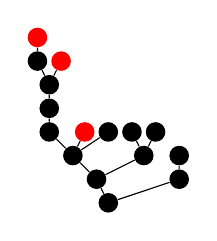
\begin{tikzpicture}[scale=.2]
\node[circle, scale=0.75, fill] (tid0) at (5.25,1.5){};
\node[circle, scale=0.75, fill] (tid1) at (4.5,3){};
\node[circle, scale=0.75, fill] (tid3) at (3,4.5){};
\node[circle, scale=0.75, fill] (tid6) at (1.5,6){};
\node[circle, scale=0.75, fill] (tid11) at (1.5,7.5){};
\node[circle, scale=0.75, fill] (tid12) at (1.5,9){};
\node[circle, scale=0.75, fill] (tid13) at (0.75,10.5){};
\node[circle, scale=0.75, fill, red] (tid15) at (0.75,12){};
\draw[](tid13) -- (tid15);
\node[circle, scale=0.75, fill, red] (tid14) at (2.25,10.5){};
\draw[](tid12) -- (tid13);
\draw[](tid12) -- (tid14);
\draw[](tid11) -- (tid12);
\draw[](tid6) -- (tid11);
\node[circle, scale=0.75, fill, red] (tid7) at (3.75,6){};
\node[circle, scale=0.75, fill] (tid8) at (5.25,6){};
\draw[](tid3) -- (tid6);
\draw[](tid3) -- (tid7);
\draw[](tid3) -- (tid8);
\node[circle, scale=0.75, fill] (tid4) at (7.5,4.5){};
\node[circle, scale=0.75, fill] (tid9) at (6.75,6){};
\node[circle, scale=0.75, fill] (tid10) at (8.25,6){};
\draw[](tid4) -- (tid9);
\draw[](tid4) -- (tid10);
\draw[](tid1) -- (tid3);
\draw[](tid1) -- (tid4);
\node[circle, scale=0.75, fill] (tid2) at (9.75,3){};
\node[circle, scale=0.75, fill] (tid5) at (9.75,4.5){};
\draw[](tid2) -- (tid5);
\draw[](tid0) -- (tid1);
\draw[](tid0) -- (tid2);
\end{tikzpicture}
\nodepart{two}
\footnotesize{882488317/102036672}
\nodepart{three}
\footnotesize{$100/9\:200/9\:100/9\:200/9\:100/3$}
};
 & 
\node[draw=black, rectangle split,  rectangle split parts=3] (sn0x6c56f0){
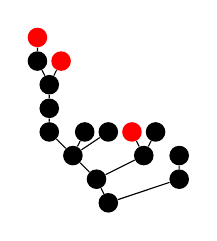
\begin{tikzpicture}[scale=.2]
\node[circle, scale=0.75, fill] (tid0) at (5.25,1.5){};
\node[circle, scale=0.75, fill] (tid1) at (4.5,3){};
\node[circle, scale=0.75, fill] (tid3) at (3,4.5){};
\node[circle, scale=0.75, fill] (tid6) at (1.5,6){};
\node[circle, scale=0.75, fill] (tid11) at (1.5,7.5){};
\node[circle, scale=0.75, fill] (tid12) at (1.5,9){};
\node[circle, scale=0.75, fill] (tid13) at (0.75,10.5){};
\node[circle, scale=0.75, fill, red] (tid15) at (0.75,12){};
\draw[](tid13) -- (tid15);
\node[circle, scale=0.75, fill, red] (tid14) at (2.25,10.5){};
\draw[](tid12) -- (tid13);
\draw[](tid12) -- (tid14);
\draw[](tid11) -- (tid12);
\draw[](tid6) -- (tid11);
\node[circle, scale=0.75, fill] (tid7) at (3.75,6){};
\node[circle, scale=0.75, fill] (tid8) at (5.25,6){};
\draw[](tid3) -- (tid6);
\draw[](tid3) -- (tid7);
\draw[](tid3) -- (tid8);
\node[circle, scale=0.75, fill] (tid4) at (7.5,4.5){};
\node[circle, scale=0.75, fill, red] (tid9) at (6.75,6){};
\node[circle, scale=0.75, fill] (tid10) at (8.25,6){};
\draw[](tid4) -- (tid9);
\draw[](tid4) -- (tid10);
\draw[](tid1) -- (tid3);
\draw[](tid1) -- (tid4);
\node[circle, scale=0.75, fill] (tid2) at (9.75,3){};
\node[circle, scale=0.75, fill] (tid5) at (9.75,4.5){};
\draw[](tid2) -- (tid5);
\draw[](tid0) -- (tid1);
\draw[](tid0) -- (tid2);
\end{tikzpicture}
\nodepart{two}
\footnotesize{7057126639/816293376}
\nodepart{three}
\footnotesize{$200/9\:200/9\:100/9\:100/9\:100/3$}
};
 & 
\node[draw=black, rectangle split,  rectangle split parts=3] (sn0x6c5260){
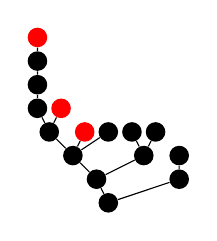
\begin{tikzpicture}[scale=.2]
\node[circle, scale=0.75, fill] (tid0) at (5.25,1.5){};
\node[circle, scale=0.75, fill] (tid1) at (4.5,3){};
\node[circle, scale=0.75, fill] (tid3) at (3,4.5){};
\node[circle, scale=0.75, fill] (tid6) at (1.5,6){};
\node[circle, scale=0.75, fill] (tid11) at (0.75,7.5){};
\node[circle, scale=0.75, fill] (tid13) at (0.75,9){};
\node[circle, scale=0.75, fill] (tid14) at (0.75,10.5){};
\node[circle, scale=0.75, fill, red] (tid15) at (0.75,12){};
\draw[](tid14) -- (tid15);
\draw[](tid13) -- (tid14);
\draw[](tid11) -- (tid13);
\node[circle, scale=0.75, fill, red] (tid12) at (2.25,7.5){};
\draw[](tid6) -- (tid11);
\draw[](tid6) -- (tid12);
\node[circle, scale=0.75, fill, red] (tid7) at (3.75,6){};
\node[circle, scale=0.75, fill] (tid8) at (5.25,6){};
\draw[](tid3) -- (tid6);
\draw[](tid3) -- (tid7);
\draw[](tid3) -- (tid8);
\node[circle, scale=0.75, fill] (tid4) at (7.5,4.5){};
\node[circle, scale=0.75, fill] (tid9) at (6.75,6){};
\node[circle, scale=0.75, fill] (tid10) at (8.25,6){};
\draw[](tid4) -- (tid9);
\draw[](tid4) -- (tid10);
\draw[](tid1) -- (tid3);
\draw[](tid1) -- (tid4);
\node[circle, scale=0.75, fill] (tid2) at (9.75,3){};
\node[circle, scale=0.75, fill] (tid5) at (9.75,4.5){};
\draw[](tid2) -- (tid5);
\draw[](tid0) -- (tid1);
\draw[](tid0) -- (tid2);
\end{tikzpicture}
\nodepart{two}
\footnotesize{5226976151/612220032}
\nodepart{three}
\footnotesize{$100/9\:200/9\:100/9\:200/9\:100/3$}
};
 & 
\node[draw=black, rectangle split,  rectangle split parts=3] (sn0x6c63e0){
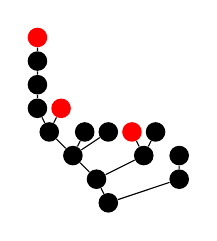
\begin{tikzpicture}[scale=.2]
\node[circle, scale=0.75, fill] (tid0) at (5.25,1.5){};
\node[circle, scale=0.75, fill] (tid1) at (4.5,3){};
\node[circle, scale=0.75, fill] (tid3) at (3,4.5){};
\node[circle, scale=0.75, fill] (tid6) at (1.5,6){};
\node[circle, scale=0.75, fill] (tid11) at (0.75,7.5){};
\node[circle, scale=0.75, fill] (tid13) at (0.75,9){};
\node[circle, scale=0.75, fill] (tid14) at (0.75,10.5){};
\node[circle, scale=0.75, fill, red] (tid15) at (0.75,12){};
\draw[](tid14) -- (tid15);
\draw[](tid13) -- (tid14);
\draw[](tid11) -- (tid13);
\node[circle, scale=0.75, fill, red] (tid12) at (2.25,7.5){};
\draw[](tid6) -- (tid11);
\draw[](tid6) -- (tid12);
\node[circle, scale=0.75, fill] (tid7) at (3.75,6){};
\node[circle, scale=0.75, fill] (tid8) at (5.25,6){};
\draw[](tid3) -- (tid6);
\draw[](tid3) -- (tid7);
\draw[](tid3) -- (tid8);
\node[circle, scale=0.75, fill] (tid4) at (7.5,4.5){};
\node[circle, scale=0.75, fill, red] (tid9) at (6.75,6){};
\node[circle, scale=0.75, fill] (tid10) at (8.25,6){};
\draw[](tid4) -- (tid9);
\draw[](tid4) -- (tid10);
\draw[](tid1) -- (tid3);
\draw[](tid1) -- (tid4);
\node[circle, scale=0.75, fill] (tid2) at (9.75,3){};
\node[circle, scale=0.75, fill] (tid5) at (9.75,4.5){};
\draw[](tid2) -- (tid5);
\draw[](tid0) -- (tid1);
\draw[](tid0) -- (tid2);
\end{tikzpicture}
\nodepart{two}
\footnotesize{6966595627/816293376}
\nodepart{three}
\footnotesize{$200/9\:100/9\:200/9\:100/9\:100/3$}
};
 & 
\node[draw=black, rectangle split,  rectangle split parts=3] (sn0x6c5c30){
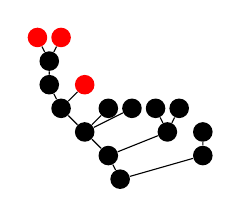
\begin{tikzpicture}[scale=.2]
\node[circle, scale=0.75, fill] (tid0) at (6,1.5){};
\node[circle, scale=0.75, fill] (tid1) at (5.25,3){};
\node[circle, scale=0.75, fill] (tid3) at (3.75,4.5){};
\node[circle, scale=0.75, fill] (tid6) at (2.25,6){};
\node[circle, scale=0.75, fill] (tid11) at (1.5,7.5){};
\node[circle, scale=0.75, fill] (tid13) at (1.5,9){};
\node[circle, scale=0.75, fill, red] (tid14) at (0.75,10.5){};
\node[circle, scale=0.75, fill, red] (tid15) at (2.25,10.5){};
\draw[](tid13) -- (tid14);
\draw[](tid13) -- (tid15);
\draw[](tid11) -- (tid13);
\node[circle, scale=0.75, fill, red] (tid12) at (3.75,7.5){};
\draw[](tid6) -- (tid11);
\draw[](tid6) -- (tid12);
\node[circle, scale=0.75, fill] (tid7) at (5.25,6){};
\node[circle, scale=0.75, fill] (tid8) at (6.75,6){};
\draw[](tid3) -- (tid6);
\draw[](tid3) -- (tid7);
\draw[](tid3) -- (tid8);
\node[circle, scale=0.75, fill] (tid4) at (9,4.5){};
\node[circle, scale=0.75, fill] (tid9) at (8.25,6){};
\node[circle, scale=0.75, fill] (tid10) at (9.75,6){};
\draw[](tid4) -- (tid9);
\draw[](tid4) -- (tid10);
\draw[](tid1) -- (tid3);
\draw[](tid1) -- (tid4);
\node[circle, scale=0.75, fill] (tid2) at (11.25,3){};
\node[circle, scale=0.75, fill] (tid5) at (11.25,4.5){};
\draw[](tid2) -- (tid5);
\draw[](tid0) -- (tid1);
\draw[](tid0) -- (tid2);
\end{tikzpicture}
\nodepart{two}
\footnotesize{2520309997/306110016}
\nodepart{three}
\footnotesize{$50/3\:50/3\:100/3\:100/3$}
};
 & 
\\
};
\end{scope}
\begin{scope}[yshift=\leveltopIII cm]
\matrix (line3) [column sep=1cm] {
\node[draw=black, rectangle split,  rectangle split parts=3] (sn0x6c9940){
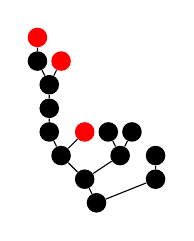
\begin{tikzpicture}[scale=.2]
\node[circle, scale=0.75, fill] (tid0) at (4.5,1.5){};
\node[circle, scale=0.75, fill] (tid1) at (3.75,3){};
\node[circle, scale=0.75, fill] (tid3) at (2.25,4.5){};
\node[circle, scale=0.75, fill] (tid6) at (1.5,6){};
\node[circle, scale=0.75, fill] (tid10) at (1.5,7.5){};
\node[circle, scale=0.75, fill] (tid11) at (1.5,9){};
\node[circle, scale=0.75, fill] (tid12) at (0.75,10.5){};
\node[circle, scale=0.75, fill, red] (tid14) at (0.75,12){};
\draw[](tid12) -- (tid14);
\node[circle, scale=0.75, fill, red] (tid13) at (2.25,10.5){};
\draw[](tid11) -- (tid12);
\draw[](tid11) -- (tid13);
\draw[](tid10) -- (tid11);
\draw[](tid6) -- (tid10);
\node[circle, scale=0.75, fill, red] (tid7) at (3.75,6){};
\draw[](tid3) -- (tid6);
\draw[](tid3) -- (tid7);
\node[circle, scale=0.75, fill] (tid4) at (6,4.5){};
\node[circle, scale=0.75, fill] (tid8) at (5.25,6){};
\node[circle, scale=0.75, fill] (tid9) at (6.75,6){};
\draw[](tid4) -- (tid8);
\draw[](tid4) -- (tid9);
\draw[](tid1) -- (tid3);
\draw[](tid1) -- (tid4);
\node[circle, scale=0.75, fill] (tid2) at (8.25,3){};
\node[circle, scale=0.75, fill] (tid5) at (8.25,4.5){};
\draw[](tid2) -- (tid5);
\draw[](tid0) -- (tid1);
\draw[](tid0) -- (tid2);
\end{tikzpicture}
\nodepart{two}
\footnotesize{386820889/45349632}
\nodepart{three}
\footnotesize{$100/3\:100/3\:100/3$}
};
 & 
\node[draw=black, rectangle split,  rectangle split parts=3] (sn0x6c67e0){
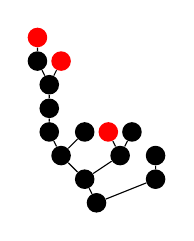
\begin{tikzpicture}[scale=.2]
\node[circle, scale=0.75, fill] (tid0) at (4.5,1.5){};
\node[circle, scale=0.75, fill] (tid1) at (3.75,3){};
\node[circle, scale=0.75, fill] (tid3) at (2.25,4.5){};
\node[circle, scale=0.75, fill] (tid6) at (1.5,6){};
\node[circle, scale=0.75, fill] (tid10) at (1.5,7.5){};
\node[circle, scale=0.75, fill] (tid11) at (1.5,9){};
\node[circle, scale=0.75, fill] (tid12) at (0.75,10.5){};
\node[circle, scale=0.75, fill, red] (tid14) at (0.75,12){};
\draw[](tid12) -- (tid14);
\node[circle, scale=0.75, fill, red] (tid13) at (2.25,10.5){};
\draw[](tid11) -- (tid12);
\draw[](tid11) -- (tid13);
\draw[](tid10) -- (tid11);
\draw[](tid6) -- (tid10);
\node[circle, scale=0.75, fill] (tid7) at (3.75,6){};
\draw[](tid3) -- (tid6);
\draw[](tid3) -- (tid7);
\node[circle, scale=0.75, fill] (tid4) at (6,4.5){};
\node[circle, scale=0.75, fill, red] (tid8) at (5.25,6){};
\node[circle, scale=0.75, fill] (tid9) at (6.75,6){};
\draw[](tid4) -- (tid8);
\draw[](tid4) -- (tid9);
\draw[](tid1) -- (tid3);
\draw[](tid1) -- (tid4);
\node[circle, scale=0.75, fill] (tid2) at (8.25,3){};
\node[circle, scale=0.75, fill] (tid5) at (8.25,4.5){};
\draw[](tid2) -- (tid5);
\draw[](tid0) -- (tid1);
\draw[](tid0) -- (tid2);
\end{tikzpicture}
\nodepart{two}
\footnotesize{386652509/45349632}
\nodepart{three}
\footnotesize{$50/3\:50/3\:50/3\:50/3\:100/3$}
};
 & 
\node[draw=black, rectangle split,  rectangle split parts=3] (sn0x6ca8e0){
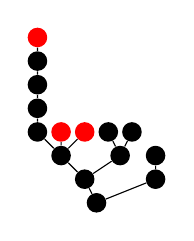
\begin{tikzpicture}[scale=.2]
\node[circle, scale=0.75, fill] (tid0) at (4.5,1.5){};
\node[circle, scale=0.75, fill] (tid1) at (3.75,3){};
\node[circle, scale=0.75, fill] (tid3) at (2.25,4.5){};
\node[circle, scale=0.75, fill] (tid6) at (0.75,6){};
\node[circle, scale=0.75, fill] (tid11) at (0.75,7.5){};
\node[circle, scale=0.75, fill] (tid12) at (0.75,9){};
\node[circle, scale=0.75, fill] (tid13) at (0.75,10.5){};
\node[circle, scale=0.75, fill, red] (tid14) at (0.75,12){};
\draw[](tid13) -- (tid14);
\draw[](tid12) -- (tid13);
\draw[](tid11) -- (tid12);
\draw[](tid6) -- (tid11);
\node[circle, scale=0.75, fill, red] (tid7) at (2.25,6){};
\node[circle, scale=0.75, fill, red] (tid8) at (3.75,6){};
\draw[](tid3) -- (tid6);
\draw[](tid3) -- (tid7);
\draw[](tid3) -- (tid8);
\node[circle, scale=0.75, fill] (tid4) at (6,4.5){};
\node[circle, scale=0.75, fill] (tid9) at (5.25,6){};
\node[circle, scale=0.75, fill] (tid10) at (6.75,6){};
\draw[](tid4) -- (tid9);
\draw[](tid4) -- (tid10);
\draw[](tid1) -- (tid3);
\draw[](tid1) -- (tid4);
\node[circle, scale=0.75, fill] (tid2) at (8.25,3){};
\node[circle, scale=0.75, fill] (tid5) at (8.25,4.5){};
\draw[](tid2) -- (tid5);
\draw[](tid0) -- (tid1);
\draw[](tid0) -- (tid2);
\end{tikzpicture}
\nodepart{two}
\footnotesize{1140633527/136048896}
\nodepart{three}
\footnotesize{$200/3\:100/3$}
};
 & 
\node[draw=black, rectangle split,  rectangle split parts=3] (sn0x6c8b90){
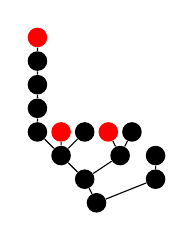
\begin{tikzpicture}[scale=.2]
\node[circle, scale=0.75, fill] (tid0) at (4.5,1.5){};
\node[circle, scale=0.75, fill] (tid1) at (3.75,3){};
\node[circle, scale=0.75, fill] (tid3) at (2.25,4.5){};
\node[circle, scale=0.75, fill] (tid6) at (0.75,6){};
\node[circle, scale=0.75, fill] (tid11) at (0.75,7.5){};
\node[circle, scale=0.75, fill] (tid12) at (0.75,9){};
\node[circle, scale=0.75, fill] (tid13) at (0.75,10.5){};
\node[circle, scale=0.75, fill, red] (tid14) at (0.75,12){};
\draw[](tid13) -- (tid14);
\draw[](tid12) -- (tid13);
\draw[](tid11) -- (tid12);
\draw[](tid6) -- (tid11);
\node[circle, scale=0.75, fill, red] (tid7) at (2.25,6){};
\node[circle, scale=0.75, fill] (tid8) at (3.75,6){};
\draw[](tid3) -- (tid6);
\draw[](tid3) -- (tid7);
\draw[](tid3) -- (tid8);
\node[circle, scale=0.75, fill] (tid4) at (6,4.5){};
\node[circle, scale=0.75, fill, red] (tid9) at (5.25,6){};
\node[circle, scale=0.75, fill] (tid10) at (6.75,6){};
\draw[](tid4) -- (tid9);
\draw[](tid4) -- (tid10);
\draw[](tid1) -- (tid3);
\draw[](tid1) -- (tid4);
\node[circle, scale=0.75, fill] (tid2) at (8.25,3){};
\node[circle, scale=0.75, fill] (tid5) at (8.25,4.5){};
\draw[](tid2) -- (tid5);
\draw[](tid0) -- (tid1);
\draw[](tid0) -- (tid2);
\end{tikzpicture}
\nodepart{two}
\footnotesize{63342067/7558272}
\nodepart{three}
\footnotesize{$50/3\:50/3\:50/3\:50/3\:100/3$}
};
 & 
\node[draw=black, rectangle split,  rectangle split parts=3] (sn0x6ca380){
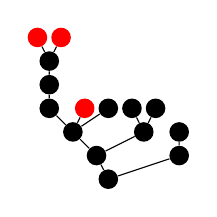
\begin{tikzpicture}[scale=.2]
\node[circle, scale=0.75, fill] (tid0) at (5.25,1.5){};
\node[circle, scale=0.75, fill] (tid1) at (4.5,3){};
\node[circle, scale=0.75, fill] (tid3) at (3,4.5){};
\node[circle, scale=0.75, fill] (tid6) at (1.5,6){};
\node[circle, scale=0.75, fill] (tid11) at (1.5,7.5){};
\node[circle, scale=0.75, fill] (tid12) at (1.5,9){};
\node[circle, scale=0.75, fill, red] (tid13) at (0.75,10.5){};
\node[circle, scale=0.75, fill, red] (tid14) at (2.25,10.5){};
\draw[](tid12) -- (tid13);
\draw[](tid12) -- (tid14);
\draw[](tid11) -- (tid12);
\draw[](tid6) -- (tid11);
\node[circle, scale=0.75, fill, red] (tid7) at (3.75,6){};
\node[circle, scale=0.75, fill] (tid8) at (5.25,6){};
\draw[](tid3) -- (tid6);
\draw[](tid3) -- (tid7);
\draw[](tid3) -- (tid8);
\node[circle, scale=0.75, fill] (tid4) at (7.5,4.5){};
\node[circle, scale=0.75, fill] (tid9) at (6.75,6){};
\node[circle, scale=0.75, fill] (tid10) at (8.25,6){};
\draw[](tid4) -- (tid9);
\draw[](tid4) -- (tid10);
\draw[](tid1) -- (tid3);
\draw[](tid1) -- (tid4);
\node[circle, scale=0.75, fill] (tid2) at (9.75,3){};
\node[circle, scale=0.75, fill] (tid5) at (9.75,4.5){};
\draw[](tid2) -- (tid5);
\draw[](tid0) -- (tid1);
\draw[](tid0) -- (tid2);
\end{tikzpicture}
\nodepart{two}
\footnotesize{25628027/3188646}
\nodepart{three}
\footnotesize{$100/9\:200/9\:200/9\:400/9$}
};
 & 
\node[draw=black, rectangle split,  rectangle split parts=3] (sn0x719c00){
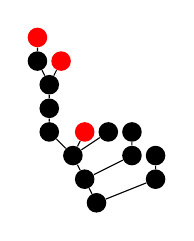
\begin{tikzpicture}[scale=.2]
\node[circle, scale=0.75, fill] (tid0) at (4.5,1.5){};
\node[circle, scale=0.75, fill] (tid1) at (3.75,3){};
\node[circle, scale=0.75, fill] (tid3) at (3,4.5){};
\node[circle, scale=0.75, fill] (tid6) at (1.5,6){};
\node[circle, scale=0.75, fill] (tid10) at (1.5,7.5){};
\node[circle, scale=0.75, fill] (tid11) at (1.5,9){};
\node[circle, scale=0.75, fill] (tid12) at (0.75,10.5){};
\node[circle, scale=0.75, fill, red] (tid14) at (0.75,12){};
\draw[](tid12) -- (tid14);
\node[circle, scale=0.75, fill, red] (tid13) at (2.25,10.5){};
\draw[](tid11) -- (tid12);
\draw[](tid11) -- (tid13);
\draw[](tid10) -- (tid11);
\draw[](tid6) -- (tid10);
\node[circle, scale=0.75, fill, red] (tid7) at (3.75,6){};
\node[circle, scale=0.75, fill] (tid8) at (5.25,6){};
\draw[](tid3) -- (tid6);
\draw[](tid3) -- (tid7);
\draw[](tid3) -- (tid8);
\node[circle, scale=0.75, fill] (tid4) at (6.75,4.5){};
\node[circle, scale=0.75, fill] (tid9) at (6.75,6){};
\draw[](tid4) -- (tid9);
\draw[](tid1) -- (tid3);
\draw[](tid1) -- (tid4);
\node[circle, scale=0.75, fill] (tid2) at (8.25,3){};
\node[circle, scale=0.75, fill] (tid5) at (8.25,4.5){};
\draw[](tid2) -- (tid5);
\draw[](tid0) -- (tid1);
\draw[](tid0) -- (tid2);
\end{tikzpicture}
\nodepart{two}
\footnotesize{257706505/30233088}
\nodepart{three}
\footnotesize{$50/3\:50/3\:50/3\:50/3\:100/3$}
};
 & 
\node[draw=black, rectangle split,  rectangle split parts=3] (sn0x71ab70){
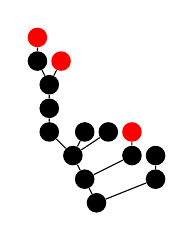
\begin{tikzpicture}[scale=.2]
\node[circle, scale=0.75, fill] (tid0) at (4.5,1.5){};
\node[circle, scale=0.75, fill] (tid1) at (3.75,3){};
\node[circle, scale=0.75, fill] (tid3) at (3,4.5){};
\node[circle, scale=0.75, fill] (tid6) at (1.5,6){};
\node[circle, scale=0.75, fill] (tid10) at (1.5,7.5){};
\node[circle, scale=0.75, fill] (tid11) at (1.5,9){};
\node[circle, scale=0.75, fill] (tid12) at (0.75,10.5){};
\node[circle, scale=0.75, fill, red] (tid14) at (0.75,12){};
\draw[](tid12) -- (tid14);
\node[circle, scale=0.75, fill, red] (tid13) at (2.25,10.5){};
\draw[](tid11) -- (tid12);
\draw[](tid11) -- (tid13);
\draw[](tid10) -- (tid11);
\draw[](tid6) -- (tid10);
\node[circle, scale=0.75, fill] (tid7) at (3.75,6){};
\node[circle, scale=0.75, fill] (tid8) at (5.25,6){};
\draw[](tid3) -- (tid6);
\draw[](tid3) -- (tid7);
\draw[](tid3) -- (tid8);
\node[circle, scale=0.75, fill] (tid4) at (6.75,4.5){};
\node[circle, scale=0.75, fill, red] (tid9) at (6.75,6){};
\draw[](tid4) -- (tid9);
\draw[](tid1) -- (tid3);
\draw[](tid1) -- (tid4);
\node[circle, scale=0.75, fill] (tid2) at (8.25,3){};
\node[circle, scale=0.75, fill] (tid5) at (8.25,4.5){};
\draw[](tid2) -- (tid5);
\draw[](tid0) -- (tid1);
\draw[](tid0) -- (tid2);
\end{tikzpicture}
\nodepart{two}
\footnotesize{257591729/30233088}
\nodepart{three}
\footnotesize{$100/3\:100/3\:100/3$}
};
 & 
\node[draw=black, rectangle split,  rectangle split parts=3] (sn0x71be10){
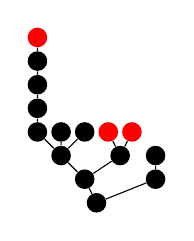
\begin{tikzpicture}[scale=.2]
\node[circle, scale=0.75, fill] (tid0) at (4.5,1.5){};
\node[circle, scale=0.75, fill] (tid1) at (3.75,3){};
\node[circle, scale=0.75, fill] (tid3) at (2.25,4.5){};
\node[circle, scale=0.75, fill] (tid6) at (0.75,6){};
\node[circle, scale=0.75, fill] (tid11) at (0.75,7.5){};
\node[circle, scale=0.75, fill] (tid12) at (0.75,9){};
\node[circle, scale=0.75, fill] (tid13) at (0.75,10.5){};
\node[circle, scale=0.75, fill, red] (tid14) at (0.75,12){};
\draw[](tid13) -- (tid14);
\draw[](tid12) -- (tid13);
\draw[](tid11) -- (tid12);
\draw[](tid6) -- (tid11);
\node[circle, scale=0.75, fill] (tid7) at (2.25,6){};
\node[circle, scale=0.75, fill] (tid8) at (3.75,6){};
\draw[](tid3) -- (tid6);
\draw[](tid3) -- (tid7);
\draw[](tid3) -- (tid8);
\node[circle, scale=0.75, fill] (tid4) at (6,4.5){};
\node[circle, scale=0.75, fill, red] (tid9) at (5.25,6){};
\node[circle, scale=0.75, fill, red] (tid10) at (6.75,6){};
\draw[](tid4) -- (tid9);
\draw[](tid4) -- (tid10);
\draw[](tid1) -- (tid3);
\draw[](tid1) -- (tid4);
\node[circle, scale=0.75, fill] (tid2) at (8.25,3){};
\node[circle, scale=0.75, fill] (tid5) at (8.25,4.5){};
\draw[](tid2) -- (tid5);
\draw[](tid0) -- (tid1);
\draw[](tid0) -- (tid2);
\end{tikzpicture}
\nodepart{two}
\footnotesize{379889287/45349632}
\nodepart{three}
\footnotesize{$200/3\:100/3$}
};
 & 
\node[draw=black, rectangle split,  rectangle split parts=3] (sn0x71bfc0){
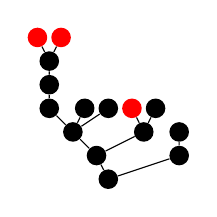
\begin{tikzpicture}[scale=.2]
\node[circle, scale=0.75, fill] (tid0) at (5.25,1.5){};
\node[circle, scale=0.75, fill] (tid1) at (4.5,3){};
\node[circle, scale=0.75, fill] (tid3) at (3,4.5){};
\node[circle, scale=0.75, fill] (tid6) at (1.5,6){};
\node[circle, scale=0.75, fill] (tid11) at (1.5,7.5){};
\node[circle, scale=0.75, fill] (tid12) at (1.5,9){};
\node[circle, scale=0.75, fill, red] (tid13) at (0.75,10.5){};
\node[circle, scale=0.75, fill, red] (tid14) at (2.25,10.5){};
\draw[](tid12) -- (tid13);
\draw[](tid12) -- (tid14);
\draw[](tid11) -- (tid12);
\draw[](tid6) -- (tid11);
\node[circle, scale=0.75, fill] (tid7) at (3.75,6){};
\node[circle, scale=0.75, fill] (tid8) at (5.25,6){};
\draw[](tid3) -- (tid6);
\draw[](tid3) -- (tid7);
\draw[](tid3) -- (tid8);
\node[circle, scale=0.75, fill] (tid4) at (7.5,4.5){};
\node[circle, scale=0.75, fill, red] (tid9) at (6.75,6){};
\node[circle, scale=0.75, fill] (tid10) at (8.25,6){};
\draw[](tid4) -- (tid9);
\draw[](tid4) -- (tid10);
\draw[](tid1) -- (tid3);
\draw[](tid1) -- (tid4);
\node[circle, scale=0.75, fill] (tid2) at (9.75,3){};
\node[circle, scale=0.75, fill] (tid5) at (9.75,4.5){};
\draw[](tid2) -- (tid5);
\draw[](tid0) -- (tid1);
\draw[](tid0) -- (tid2);
\end{tikzpicture}
\nodepart{two}
\footnotesize{136626653/17006112}
\nodepart{three}
\footnotesize{$400/9\:200/9\:100/9\:200/9$}
};
 & 
\node[draw=black, rectangle split,  rectangle split parts=3] (sn0x722240){
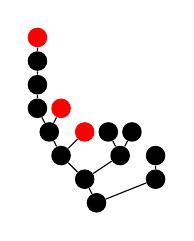
\begin{tikzpicture}[scale=.2]
\node[circle, scale=0.75, fill] (tid0) at (4.5,1.5){};
\node[circle, scale=0.75, fill] (tid1) at (3.75,3){};
\node[circle, scale=0.75, fill] (tid3) at (2.25,4.5){};
\node[circle, scale=0.75, fill] (tid6) at (1.5,6){};
\node[circle, scale=0.75, fill] (tid10) at (0.75,7.5){};
\node[circle, scale=0.75, fill] (tid12) at (0.75,9){};
\node[circle, scale=0.75, fill] (tid13) at (0.75,10.5){};
\node[circle, scale=0.75, fill, red] (tid14) at (0.75,12){};
\draw[](tid13) -- (tid14);
\draw[](tid12) -- (tid13);
\draw[](tid10) -- (tid12);
\node[circle, scale=0.75, fill, red] (tid11) at (2.25,7.5){};
\draw[](tid6) -- (tid10);
\draw[](tid6) -- (tid11);
\node[circle, scale=0.75, fill, red] (tid7) at (3.75,6){};
\draw[](tid3) -- (tid6);
\draw[](tid3) -- (tid7);
\node[circle, scale=0.75, fill] (tid4) at (6,4.5){};
\node[circle, scale=0.75, fill] (tid8) at (5.25,6){};
\node[circle, scale=0.75, fill] (tid9) at (6.75,6){};
\draw[](tid4) -- (tid8);
\draw[](tid4) -- (tid9);
\draw[](tid1) -- (tid3);
\draw[](tid1) -- (tid4);
\node[circle, scale=0.75, fill] (tid2) at (8.25,3){};
\node[circle, scale=0.75, fill] (tid5) at (8.25,4.5){};
\draw[](tid2) -- (tid5);
\draw[](tid0) -- (tid1);
\draw[](tid0) -- (tid2);
\end{tikzpicture}
\nodepart{two}
\footnotesize{380943829/45349632}
\nodepart{three}
\footnotesize{$100/3\:100/3\:100/3$}
};
 & 
\node[draw=black, rectangle split,  rectangle split parts=3] (sn0x721cf0){
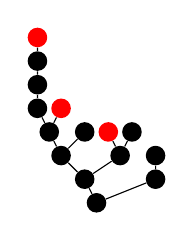
\begin{tikzpicture}[scale=.2]
\node[circle, scale=0.75, fill] (tid0) at (4.5,1.5){};
\node[circle, scale=0.75, fill] (tid1) at (3.75,3){};
\node[circle, scale=0.75, fill] (tid3) at (2.25,4.5){};
\node[circle, scale=0.75, fill] (tid6) at (1.5,6){};
\node[circle, scale=0.75, fill] (tid10) at (0.75,7.5){};
\node[circle, scale=0.75, fill] (tid12) at (0.75,9){};
\node[circle, scale=0.75, fill] (tid13) at (0.75,10.5){};
\node[circle, scale=0.75, fill, red] (tid14) at (0.75,12){};
\draw[](tid13) -- (tid14);
\draw[](tid12) -- (tid13);
\draw[](tid10) -- (tid12);
\node[circle, scale=0.75, fill, red] (tid11) at (2.25,7.5){};
\draw[](tid6) -- (tid10);
\draw[](tid6) -- (tid11);
\node[circle, scale=0.75, fill] (tid7) at (3.75,6){};
\draw[](tid3) -- (tid6);
\draw[](tid3) -- (tid7);
\node[circle, scale=0.75, fill] (tid4) at (6,4.5){};
\node[circle, scale=0.75, fill, red] (tid8) at (5.25,6){};
\node[circle, scale=0.75, fill] (tid9) at (6.75,6){};
\draw[](tid4) -- (tid8);
\draw[](tid4) -- (tid9);
\draw[](tid1) -- (tid3);
\draw[](tid1) -- (tid4);
\node[circle, scale=0.75, fill] (tid2) at (8.25,3){};
\node[circle, scale=0.75, fill] (tid5) at (8.25,4.5){};
\draw[](tid2) -- (tid5);
\draw[](tid0) -- (tid1);
\draw[](tid0) -- (tid2);
\end{tikzpicture}
\nodepart{two}
\footnotesize{190388999/22674816}
\nodepart{three}
\footnotesize{$50/3\:50/3\:50/3\:50/3\:100/3$}
};
 & 
\node[draw=black, rectangle split,  rectangle split parts=3] (sn0x721b10){
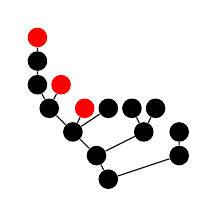
\begin{tikzpicture}[scale=.2]
\node[circle, scale=0.75, fill] (tid0) at (5.25,1.5){};
\node[circle, scale=0.75, fill] (tid1) at (4.5,3){};
\node[circle, scale=0.75, fill] (tid3) at (3,4.5){};
\node[circle, scale=0.75, fill] (tid6) at (1.5,6){};
\node[circle, scale=0.75, fill] (tid11) at (0.75,7.5){};
\node[circle, scale=0.75, fill] (tid13) at (0.75,9){};
\node[circle, scale=0.75, fill, red] (tid14) at (0.75,10.5){};
\draw[](tid13) -- (tid14);
\draw[](tid11) -- (tid13);
\node[circle, scale=0.75, fill, red] (tid12) at (2.25,7.5){};
\draw[](tid6) -- (tid11);
\draw[](tid6) -- (tid12);
\node[circle, scale=0.75, fill, red] (tid7) at (3.75,6){};
\node[circle, scale=0.75, fill] (tid8) at (5.25,6){};
\draw[](tid3) -- (tid6);
\draw[](tid3) -- (tid7);
\draw[](tid3) -- (tid8);
\node[circle, scale=0.75, fill] (tid4) at (7.5,4.5){};
\node[circle, scale=0.75, fill] (tid9) at (6.75,6){};
\node[circle, scale=0.75, fill] (tid10) at (8.25,6){};
\draw[](tid4) -- (tid9);
\draw[](tid4) -- (tid10);
\draw[](tid1) -- (tid3);
\draw[](tid1) -- (tid4);
\node[circle, scale=0.75, fill] (tid2) at (9.75,3){};
\node[circle, scale=0.75, fill] (tid5) at (9.75,4.5){};
\draw[](tid2) -- (tid5);
\draw[](tid0) -- (tid1);
\draw[](tid0) -- (tid2);
\end{tikzpicture}
\nodepart{two}
\footnotesize{399669775/51018336}
\nodepart{three}
\footnotesize{$100/9\:200/9\:100/9\:200/9\:100/3$}
};
 & 
\node[draw=black, rectangle split,  rectangle split parts=3] (sn0x740a50){
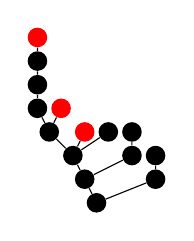
\begin{tikzpicture}[scale=.2]
\node[circle, scale=0.75, fill] (tid0) at (4.5,1.5){};
\node[circle, scale=0.75, fill] (tid1) at (3.75,3){};
\node[circle, scale=0.75, fill] (tid3) at (3,4.5){};
\node[circle, scale=0.75, fill] (tid6) at (1.5,6){};
\node[circle, scale=0.75, fill] (tid10) at (0.75,7.5){};
\node[circle, scale=0.75, fill] (tid12) at (0.75,9){};
\node[circle, scale=0.75, fill] (tid13) at (0.75,10.5){};
\node[circle, scale=0.75, fill, red] (tid14) at (0.75,12){};
\draw[](tid13) -- (tid14);
\draw[](tid12) -- (tid13);
\draw[](tid10) -- (tid12);
\node[circle, scale=0.75, fill, red] (tid11) at (2.25,7.5){};
\draw[](tid6) -- (tid10);
\draw[](tid6) -- (tid11);
\node[circle, scale=0.75, fill, red] (tid7) at (3.75,6){};
\node[circle, scale=0.75, fill] (tid8) at (5.25,6){};
\draw[](tid3) -- (tid6);
\draw[](tid3) -- (tid7);
\draw[](tid3) -- (tid8);
\node[circle, scale=0.75, fill] (tid4) at (6.75,4.5){};
\node[circle, scale=0.75, fill] (tid9) at (6.75,6){};
\draw[](tid4) -- (tid9);
\draw[](tid1) -- (tid3);
\draw[](tid1) -- (tid4);
\node[circle, scale=0.75, fill] (tid2) at (8.25,3){};
\node[circle, scale=0.75, fill] (tid5) at (8.25,4.5){};
\draw[](tid2) -- (tid5);
\draw[](tid0) -- (tid1);
\draw[](tid0) -- (tid2);
\end{tikzpicture}
\nodepart{two}
\footnotesize{253797211/30233088}
\nodepart{three}
\footnotesize{$50/3\:50/3\:50/3\:50/3\:100/3$}
};
 & 
\node[draw=black, rectangle split,  rectangle split parts=3] (sn0x743740){
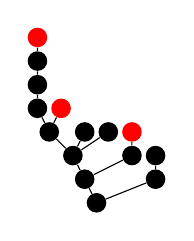
\begin{tikzpicture}[scale=.2]
\node[circle, scale=0.75, fill] (tid0) at (4.5,1.5){};
\node[circle, scale=0.75, fill] (tid1) at (3.75,3){};
\node[circle, scale=0.75, fill] (tid3) at (3,4.5){};
\node[circle, scale=0.75, fill] (tid6) at (1.5,6){};
\node[circle, scale=0.75, fill] (tid10) at (0.75,7.5){};
\node[circle, scale=0.75, fill] (tid12) at (0.75,9){};
\node[circle, scale=0.75, fill] (tid13) at (0.75,10.5){};
\node[circle, scale=0.75, fill, red] (tid14) at (0.75,12){};
\draw[](tid13) -- (tid14);
\draw[](tid12) -- (tid13);
\draw[](tid10) -- (tid12);
\node[circle, scale=0.75, fill, red] (tid11) at (2.25,7.5){};
\draw[](tid6) -- (tid10);
\draw[](tid6) -- (tid11);
\node[circle, scale=0.75, fill] (tid7) at (3.75,6){};
\node[circle, scale=0.75, fill] (tid8) at (5.25,6){};
\draw[](tid3) -- (tid6);
\draw[](tid3) -- (tid7);
\draw[](tid3) -- (tid8);
\node[circle, scale=0.75, fill] (tid4) at (6.75,4.5){};
\node[circle, scale=0.75, fill, red] (tid9) at (6.75,6){};
\draw[](tid4) -- (tid9);
\draw[](tid1) -- (tid3);
\draw[](tid1) -- (tid4);
\node[circle, scale=0.75, fill] (tid2) at (8.25,3){};
\node[circle, scale=0.75, fill] (tid5) at (8.25,4.5){};
\draw[](tid2) -- (tid5);
\draw[](tid0) -- (tid1);
\draw[](tid0) -- (tid2);
\end{tikzpicture}
\nodepart{two}
\footnotesize{761045363/90699264}
\nodepart{three}
\footnotesize{$100/3\:100/3\:100/3$}
};
 & 
\node[draw=black, rectangle split,  rectangle split parts=3] (sn0x741de0){
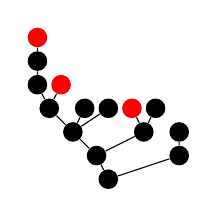
\begin{tikzpicture}[scale=.2]
\node[circle, scale=0.75, fill] (tid0) at (5.25,1.5){};
\node[circle, scale=0.75, fill] (tid1) at (4.5,3){};
\node[circle, scale=0.75, fill] (tid3) at (3,4.5){};
\node[circle, scale=0.75, fill] (tid6) at (1.5,6){};
\node[circle, scale=0.75, fill] (tid11) at (0.75,7.5){};
\node[circle, scale=0.75, fill] (tid13) at (0.75,9){};
\node[circle, scale=0.75, fill, red] (tid14) at (0.75,10.5){};
\draw[](tid13) -- (tid14);
\draw[](tid11) -- (tid13);
\node[circle, scale=0.75, fill, red] (tid12) at (2.25,7.5){};
\draw[](tid6) -- (tid11);
\draw[](tid6) -- (tid12);
\node[circle, scale=0.75, fill] (tid7) at (3.75,6){};
\node[circle, scale=0.75, fill] (tid8) at (5.25,6){};
\draw[](tid3) -- (tid6);
\draw[](tid3) -- (tid7);
\draw[](tid3) -- (tid8);
\node[circle, scale=0.75, fill] (tid4) at (7.5,4.5){};
\node[circle, scale=0.75, fill, red] (tid9) at (6.75,6){};
\node[circle, scale=0.75, fill] (tid10) at (8.25,6){};
\draw[](tid4) -- (tid9);
\draw[](tid4) -- (tid10);
\draw[](tid1) -- (tid3);
\draw[](tid1) -- (tid4);
\node[circle, scale=0.75, fill] (tid2) at (9.75,3){};
\node[circle, scale=0.75, fill] (tid5) at (9.75,4.5){};
\draw[](tid2) -- (tid5);
\draw[](tid0) -- (tid1);
\draw[](tid0) -- (tid2);
\end{tikzpicture}
\nodepart{two}
\footnotesize{411011/52488}
\nodepart{three}
\footnotesize{$200/9\:100/9\:200/9\:100/9\:100/3$}
};
 & 
\\
};
\end{scope}
\begin{scope}[yshift=\leveltopIIII cm]
\matrix (line4) [column sep=1cm] {
\node[draw=black, rectangle split,  rectangle split parts=3] (sn0x6ca9b0){
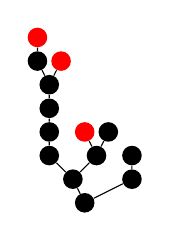
\begin{tikzpicture}[scale=.2]
\node[circle, scale=0.75, fill] (tid0) at (3.75,1.5){};
\node[circle, scale=0.75, fill] (tid1) at (3,3){};
\node[circle, scale=0.75, fill] (tid3) at (1.5,4.5){};
\node[circle, scale=0.75, fill] (tid6) at (1.5,6){};
\node[circle, scale=0.75, fill] (tid9) at (1.5,7.5){};
\node[circle, scale=0.75, fill] (tid10) at (1.5,9){};
\node[circle, scale=0.75, fill] (tid11) at (0.75,10.5){};
\node[circle, scale=0.75, fill, red] (tid13) at (0.75,12){};
\draw[](tid11) -- (tid13);
\node[circle, scale=0.75, fill, red] (tid12) at (2.25,10.5){};
\draw[](tid10) -- (tid11);
\draw[](tid10) -- (tid12);
\draw[](tid9) -- (tid10);
\draw[](tid6) -- (tid9);
\draw[](tid3) -- (tid6);
\node[circle, scale=0.75, fill] (tid4) at (4.5,4.5){};
\node[circle, scale=0.75, fill, red] (tid7) at (3.75,6){};
\node[circle, scale=0.75, fill] (tid8) at (5.25,6){};
\draw[](tid4) -- (tid7);
\draw[](tid4) -- (tid8);
\draw[](tid1) -- (tid3);
\draw[](tid1) -- (tid4);
\node[circle, scale=0.75, fill] (tid2) at (6.75,3){};
\node[circle, scale=0.75, fill] (tid5) at (6.75,4.5){};
\draw[](tid2) -- (tid5);
\draw[](tid0) -- (tid1);
\draw[](tid0) -- (tid2);
\end{tikzpicture}
\nodepart{two}
\footnotesize{85014691/10077696}
\nodepart{three}
\footnotesize{$100/3\:100/3\:100/3$}
};
 & 
\node[draw=black, rectangle split,  rectangle split parts=3] (sn0x6cd1e0){
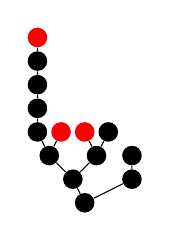
\begin{tikzpicture}[scale=.2]
\node[circle, scale=0.75, fill] (tid0) at (3.75,1.5){};
\node[circle, scale=0.75, fill] (tid1) at (3,3){};
\node[circle, scale=0.75, fill] (tid3) at (1.5,4.5){};
\node[circle, scale=0.75, fill] (tid6) at (0.75,6){};
\node[circle, scale=0.75, fill] (tid10) at (0.75,7.5){};
\node[circle, scale=0.75, fill] (tid11) at (0.75,9){};
\node[circle, scale=0.75, fill] (tid12) at (0.75,10.5){};
\node[circle, scale=0.75, fill, red] (tid13) at (0.75,12){};
\draw[](tid12) -- (tid13);
\draw[](tid11) -- (tid12);
\draw[](tid10) -- (tid11);
\draw[](tid6) -- (tid10);
\node[circle, scale=0.75, fill, red] (tid7) at (2.25,6){};
\draw[](tid3) -- (tid6);
\draw[](tid3) -- (tid7);
\node[circle, scale=0.75, fill] (tid4) at (4.5,4.5){};
\node[circle, scale=0.75, fill, red] (tid8) at (3.75,6){};
\node[circle, scale=0.75, fill] (tid9) at (5.25,6){};
\draw[](tid4) -- (tid8);
\draw[](tid4) -- (tid9);
\draw[](tid1) -- (tid3);
\draw[](tid1) -- (tid4);
\node[circle, scale=0.75, fill] (tid2) at (6.75,3){};
\node[circle, scale=0.75, fill] (tid5) at (6.75,4.5){};
\draw[](tid2) -- (tid5);
\draw[](tid0) -- (tid1);
\draw[](tid0) -- (tid2);
\end{tikzpicture}
\nodepart{two}
\footnotesize{83319059/10077696}
\nodepart{three}
\footnotesize{$100/3\:100/3\:100/3$}
};
 & 
\node[draw=black, rectangle split,  rectangle split parts=3] (sn0x6cacd0){
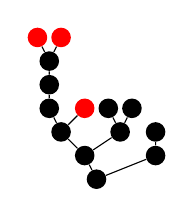
\begin{tikzpicture}[scale=.2]
\node[circle, scale=0.75, fill] (tid0) at (4.5,1.5){};
\node[circle, scale=0.75, fill] (tid1) at (3.75,3){};
\node[circle, scale=0.75, fill] (tid3) at (2.25,4.5){};
\node[circle, scale=0.75, fill] (tid6) at (1.5,6){};
\node[circle, scale=0.75, fill] (tid10) at (1.5,7.5){};
\node[circle, scale=0.75, fill] (tid11) at (1.5,9){};
\node[circle, scale=0.75, fill, red] (tid12) at (0.75,10.5){};
\node[circle, scale=0.75, fill, red] (tid13) at (2.25,10.5){};
\draw[](tid11) -- (tid12);
\draw[](tid11) -- (tid13);
\draw[](tid10) -- (tid11);
\draw[](tid6) -- (tid10);
\node[circle, scale=0.75, fill, red] (tid7) at (3.75,6){};
\draw[](tid3) -- (tid6);
\draw[](tid3) -- (tid7);
\node[circle, scale=0.75, fill] (tid4) at (6,4.5){};
\node[circle, scale=0.75, fill] (tid8) at (5.25,6){};
\node[circle, scale=0.75, fill] (tid9) at (6.75,6){};
\draw[](tid4) -- (tid8);
\draw[](tid4) -- (tid9);
\draw[](tid1) -- (tid3);
\draw[](tid1) -- (tid4);
\node[circle, scale=0.75, fill] (tid2) at (8.25,3){};
\node[circle, scale=0.75, fill] (tid5) at (8.25,4.5){};
\draw[](tid2) -- (tid5);
\draw[](tid0) -- (tid1);
\draw[](tid0) -- (tid2);
\end{tikzpicture}
\nodepart{two}
\footnotesize{14900465/1889568}
\nodepart{three}
\footnotesize{$100/3\:200/3$}
};
 & 
\node[draw=black, rectangle split,  rectangle split parts=3] (sn0x703050){
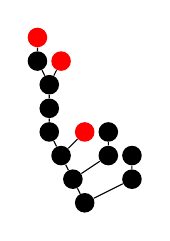
\begin{tikzpicture}[scale=.2]
\node[circle, scale=0.75, fill] (tid0) at (3.75,1.5){};
\node[circle, scale=0.75, fill] (tid1) at (3,3){};
\node[circle, scale=0.75, fill] (tid3) at (2.25,4.5){};
\node[circle, scale=0.75, fill] (tid6) at (1.5,6){};
\node[circle, scale=0.75, fill] (tid9) at (1.5,7.5){};
\node[circle, scale=0.75, fill] (tid10) at (1.5,9){};
\node[circle, scale=0.75, fill] (tid11) at (0.75,10.5){};
\node[circle, scale=0.75, fill, red] (tid13) at (0.75,12){};
\draw[](tid11) -- (tid13);
\node[circle, scale=0.75, fill, red] (tid12) at (2.25,10.5){};
\draw[](tid10) -- (tid11);
\draw[](tid10) -- (tid12);
\draw[](tid9) -- (tid10);
\draw[](tid6) -- (tid9);
\node[circle, scale=0.75, fill, red] (tid7) at (3.75,6){};
\draw[](tid3) -- (tid6);
\draw[](tid3) -- (tid7);
\node[circle, scale=0.75, fill] (tid4) at (5.25,4.5){};
\node[circle, scale=0.75, fill] (tid8) at (5.25,6){};
\draw[](tid4) -- (tid8);
\draw[](tid1) -- (tid3);
\draw[](tid1) -- (tid4);
\node[circle, scale=0.75, fill] (tid2) at (6.75,3){};
\node[circle, scale=0.75, fill] (tid5) at (6.75,4.5){};
\draw[](tid2) -- (tid5);
\draw[](tid0) -- (tid1);
\draw[](tid0) -- (tid2);
\end{tikzpicture}
\nodepart{two}
\footnotesize{127462045/15116544}
\nodepart{three}
\footnotesize{$100/3\:100/3\:100/3$}
};
 & 
\node[draw=black, rectangle split,  rectangle split parts=3] (sn0x703710){
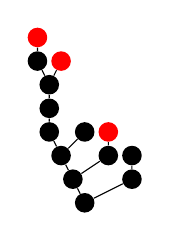
\begin{tikzpicture}[scale=.2]
\node[circle, scale=0.75, fill] (tid0) at (3.75,1.5){};
\node[circle, scale=0.75, fill] (tid1) at (3,3){};
\node[circle, scale=0.75, fill] (tid3) at (2.25,4.5){};
\node[circle, scale=0.75, fill] (tid6) at (1.5,6){};
\node[circle, scale=0.75, fill] (tid9) at (1.5,7.5){};
\node[circle, scale=0.75, fill] (tid10) at (1.5,9){};
\node[circle, scale=0.75, fill] (tid11) at (0.75,10.5){};
\node[circle, scale=0.75, fill, red] (tid13) at (0.75,12){};
\draw[](tid11) -- (tid13);
\node[circle, scale=0.75, fill, red] (tid12) at (2.25,10.5){};
\draw[](tid10) -- (tid11);
\draw[](tid10) -- (tid12);
\draw[](tid9) -- (tid10);
\draw[](tid6) -- (tid9);
\node[circle, scale=0.75, fill] (tid7) at (3.75,6){};
\draw[](tid3) -- (tid6);
\draw[](tid3) -- (tid7);
\node[circle, scale=0.75, fill] (tid4) at (5.25,4.5){};
\node[circle, scale=0.75, fill, red] (tid8) at (5.25,6){};
\draw[](tid4) -- (tid8);
\draw[](tid1) -- (tid3);
\draw[](tid1) -- (tid4);
\node[circle, scale=0.75, fill] (tid2) at (6.75,3){};
\node[circle, scale=0.75, fill] (tid5) at (6.75,4.5){};
\draw[](tid2) -- (tid5);
\draw[](tid0) -- (tid1);
\draw[](tid0) -- (tid2);
\end{tikzpicture}
\nodepart{two}
\footnotesize{3145847/373248}
\nodepart{three}
\footnotesize{$100/3\:100/3\:100/3$}
};
 & 
\node[draw=black, rectangle split,  rectangle split parts=3] (sn0x7041a0){
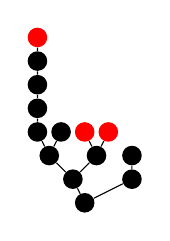
\begin{tikzpicture}[scale=.2]
\node[circle, scale=0.75, fill] (tid0) at (3.75,1.5){};
\node[circle, scale=0.75, fill] (tid1) at (3,3){};
\node[circle, scale=0.75, fill] (tid3) at (1.5,4.5){};
\node[circle, scale=0.75, fill] (tid6) at (0.75,6){};
\node[circle, scale=0.75, fill] (tid10) at (0.75,7.5){};
\node[circle, scale=0.75, fill] (tid11) at (0.75,9){};
\node[circle, scale=0.75, fill] (tid12) at (0.75,10.5){};
\node[circle, scale=0.75, fill, red] (tid13) at (0.75,12){};
\draw[](tid12) -- (tid13);
\draw[](tid11) -- (tid12);
\draw[](tid10) -- (tid11);
\draw[](tid6) -- (tid10);
\node[circle, scale=0.75, fill] (tid7) at (2.25,6){};
\draw[](tid3) -- (tid6);
\draw[](tid3) -- (tid7);
\node[circle, scale=0.75, fill] (tid4) at (4.5,4.5){};
\node[circle, scale=0.75, fill, red] (tid8) at (3.75,6){};
\node[circle, scale=0.75, fill, red] (tid9) at (5.25,6){};
\draw[](tid4) -- (tid8);
\draw[](tid4) -- (tid9);
\draw[](tid1) -- (tid3);
\draw[](tid1) -- (tid4);
\node[circle, scale=0.75, fill] (tid2) at (6.75,3){};
\node[circle, scale=0.75, fill] (tid5) at (6.75,4.5){};
\draw[](tid2) -- (tid5);
\draw[](tid0) -- (tid1);
\draw[](tid0) -- (tid2);
\end{tikzpicture}
\nodepart{two}
\footnotesize{124926397/15116544}
\nodepart{three}
\footnotesize{$200/3\:100/3$}
};
 & 
\node[draw=black, rectangle split,  rectangle split parts=3] (sn0x700a10){
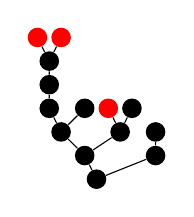
\begin{tikzpicture}[scale=.2]
\node[circle, scale=0.75, fill] (tid0) at (4.5,1.5){};
\node[circle, scale=0.75, fill] (tid1) at (3.75,3){};
\node[circle, scale=0.75, fill] (tid3) at (2.25,4.5){};
\node[circle, scale=0.75, fill] (tid6) at (1.5,6){};
\node[circle, scale=0.75, fill] (tid10) at (1.5,7.5){};
\node[circle, scale=0.75, fill] (tid11) at (1.5,9){};
\node[circle, scale=0.75, fill, red] (tid12) at (0.75,10.5){};
\node[circle, scale=0.75, fill, red] (tid13) at (2.25,10.5){};
\draw[](tid11) -- (tid12);
\draw[](tid11) -- (tid13);
\draw[](tid10) -- (tid11);
\draw[](tid6) -- (tid10);
\node[circle, scale=0.75, fill] (tid7) at (3.75,6){};
\draw[](tid3) -- (tid6);
\draw[](tid3) -- (tid7);
\node[circle, scale=0.75, fill] (tid4) at (6,4.5){};
\node[circle, scale=0.75, fill, red] (tid8) at (5.25,6){};
\node[circle, scale=0.75, fill] (tid9) at (6.75,6){};
\draw[](tid4) -- (tid8);
\draw[](tid4) -- (tid9);
\draw[](tid1) -- (tid3);
\draw[](tid1) -- (tid4);
\node[circle, scale=0.75, fill] (tid2) at (8.25,3){};
\node[circle, scale=0.75, fill] (tid5) at (8.25,4.5){};
\draw[](tid2) -- (tid5);
\draw[](tid0) -- (tid1);
\draw[](tid0) -- (tid2);
\end{tikzpicture}
\nodepart{two}
\footnotesize{14893631/1889568}
\nodepart{three}
\footnotesize{$100/3\:50/3\:50/3\:100/3$}
};
 & 
\node[draw=black, rectangle split,  rectangle split parts=3] (sn0x70ab10){
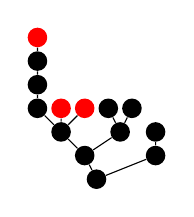
\begin{tikzpicture}[scale=.2]
\node[circle, scale=0.75, fill] (tid0) at (4.5,1.5){};
\node[circle, scale=0.75, fill] (tid1) at (3.75,3){};
\node[circle, scale=0.75, fill] (tid3) at (2.25,4.5){};
\node[circle, scale=0.75, fill] (tid6) at (0.75,6){};
\node[circle, scale=0.75, fill] (tid11) at (0.75,7.5){};
\node[circle, scale=0.75, fill] (tid12) at (0.75,9){};
\node[circle, scale=0.75, fill, red] (tid13) at (0.75,10.5){};
\draw[](tid12) -- (tid13);
\draw[](tid11) -- (tid12);
\draw[](tid6) -- (tid11);
\node[circle, scale=0.75, fill, red] (tid7) at (2.25,6){};
\node[circle, scale=0.75, fill, red] (tid8) at (3.75,6){};
\draw[](tid3) -- (tid6);
\draw[](tid3) -- (tid7);
\draw[](tid3) -- (tid8);
\node[circle, scale=0.75, fill] (tid4) at (6,4.5){};
\node[circle, scale=0.75, fill] (tid9) at (5.25,6){};
\node[circle, scale=0.75, fill] (tid10) at (6.75,6){};
\draw[](tid4) -- (tid9);
\draw[](tid4) -- (tid10);
\draw[](tid1) -- (tid3);
\draw[](tid1) -- (tid4);
\node[circle, scale=0.75, fill] (tid2) at (8.25,3){};
\node[circle, scale=0.75, fill] (tid5) at (8.25,4.5){};
\draw[](tid2) -- (tid5);
\draw[](tid0) -- (tid1);
\draw[](tid0) -- (tid2);
\end{tikzpicture}
\nodepart{two}
\footnotesize{86353091/11337408}
\nodepart{three}
\footnotesize{$200/3\:100/3$}
};
 & 
\node[draw=black, rectangle split,  rectangle split parts=3] (sn0x70fdc0){
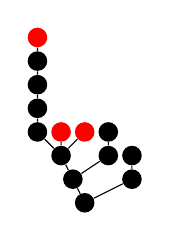
\begin{tikzpicture}[scale=.2]
\node[circle, scale=0.75, fill] (tid0) at (3.75,1.5){};
\node[circle, scale=0.75, fill] (tid1) at (3,3){};
\node[circle, scale=0.75, fill] (tid3) at (2.25,4.5){};
\node[circle, scale=0.75, fill] (tid6) at (0.75,6){};
\node[circle, scale=0.75, fill] (tid10) at (0.75,7.5){};
\node[circle, scale=0.75, fill] (tid11) at (0.75,9){};
\node[circle, scale=0.75, fill] (tid12) at (0.75,10.5){};
\node[circle, scale=0.75, fill, red] (tid13) at (0.75,12){};
\draw[](tid12) -- (tid13);
\draw[](tid11) -- (tid12);
\draw[](tid10) -- (tid11);
\draw[](tid6) -- (tid10);
\node[circle, scale=0.75, fill, red] (tid7) at (2.25,6){};
\node[circle, scale=0.75, fill, red] (tid8) at (3.75,6){};
\draw[](tid3) -- (tid6);
\draw[](tid3) -- (tid7);
\draw[](tid3) -- (tid8);
\node[circle, scale=0.75, fill] (tid4) at (5.25,4.5){};
\node[circle, scale=0.75, fill] (tid9) at (5.25,6){};
\draw[](tid4) -- (tid9);
\draw[](tid1) -- (tid3);
\draw[](tid1) -- (tid4);
\node[circle, scale=0.75, fill] (tid2) at (6.75,3){};
\node[circle, scale=0.75, fill] (tid5) at (6.75,4.5){};
\draw[](tid2) -- (tid5);
\draw[](tid0) -- (tid1);
\draw[](tid0) -- (tid2);
\end{tikzpicture}
\nodepart{two}
\footnotesize{124926221/15116544}
\nodepart{three}
\footnotesize{$200/3\:100/3$}
};
 & 
\node[draw=black, rectangle split,  rectangle split parts=3] (sn0x70e680){
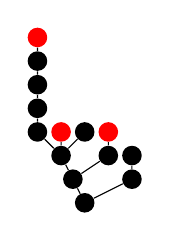
\begin{tikzpicture}[scale=.2]
\node[circle, scale=0.75, fill] (tid0) at (3.75,1.5){};
\node[circle, scale=0.75, fill] (tid1) at (3,3){};
\node[circle, scale=0.75, fill] (tid3) at (2.25,4.5){};
\node[circle, scale=0.75, fill] (tid6) at (0.75,6){};
\node[circle, scale=0.75, fill] (tid10) at (0.75,7.5){};
\node[circle, scale=0.75, fill] (tid11) at (0.75,9){};
\node[circle, scale=0.75, fill] (tid12) at (0.75,10.5){};
\node[circle, scale=0.75, fill, red] (tid13) at (0.75,12){};
\draw[](tid12) -- (tid13);
\draw[](tid11) -- (tid12);
\draw[](tid10) -- (tid11);
\draw[](tid6) -- (tid10);
\node[circle, scale=0.75, fill, red] (tid7) at (2.25,6){};
\node[circle, scale=0.75, fill] (tid8) at (3.75,6){};
\draw[](tid3) -- (tid6);
\draw[](tid3) -- (tid7);
\draw[](tid3) -- (tid8);
\node[circle, scale=0.75, fill] (tid4) at (5.25,4.5){};
\node[circle, scale=0.75, fill, red] (tid9) at (5.25,6){};
\draw[](tid4) -- (tid9);
\draw[](tid1) -- (tid3);
\draw[](tid1) -- (tid4);
\node[circle, scale=0.75, fill] (tid2) at (6.75,3){};
\node[circle, scale=0.75, fill] (tid5) at (6.75,4.5){};
\draw[](tid2) -- (tid5);
\draw[](tid0) -- (tid1);
\draw[](tid0) -- (tid2);
\end{tikzpicture}
\nodepart{two}
\footnotesize{83248297/10077696}
\nodepart{three}
\footnotesize{$100/3\:100/3\:100/3$}
};
 & 
\node[draw=black, rectangle split,  rectangle split parts=3] (sn0x70ff90){
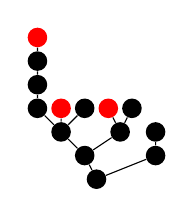
\begin{tikzpicture}[scale=.2]
\node[circle, scale=0.75, fill] (tid0) at (4.5,1.5){};
\node[circle, scale=0.75, fill] (tid1) at (3.75,3){};
\node[circle, scale=0.75, fill] (tid3) at (2.25,4.5){};
\node[circle, scale=0.75, fill] (tid6) at (0.75,6){};
\node[circle, scale=0.75, fill] (tid11) at (0.75,7.5){};
\node[circle, scale=0.75, fill] (tid12) at (0.75,9){};
\node[circle, scale=0.75, fill, red] (tid13) at (0.75,10.5){};
\draw[](tid12) -- (tid13);
\draw[](tid11) -- (tid12);
\draw[](tid6) -- (tid11);
\node[circle, scale=0.75, fill, red] (tid7) at (2.25,6){};
\node[circle, scale=0.75, fill] (tid8) at (3.75,6){};
\draw[](tid3) -- (tid6);
\draw[](tid3) -- (tid7);
\draw[](tid3) -- (tid8);
\node[circle, scale=0.75, fill] (tid4) at (6,4.5){};
\node[circle, scale=0.75, fill, red] (tid9) at (5.25,6){};
\node[circle, scale=0.75, fill] (tid10) at (6.75,6){};
\draw[](tid4) -- (tid9);
\draw[](tid4) -- (tid10);
\draw[](tid1) -- (tid3);
\draw[](tid1) -- (tid4);
\node[circle, scale=0.75, fill] (tid2) at (8.25,3){};
\node[circle, scale=0.75, fill] (tid5) at (8.25,4.5){};
\draw[](tid2) -- (tid5);
\draw[](tid0) -- (tid1);
\draw[](tid0) -- (tid2);
\end{tikzpicture}
\nodepart{two}
\footnotesize{149849/19683}
\nodepart{three}
\footnotesize{$50/3\:50/3\:50/3\:50/3\:100/3$}
};
 & 
\node[draw=black, rectangle split,  rectangle split parts=3] (sn0x71c7a0){
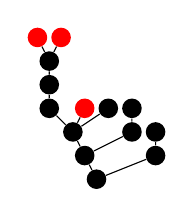
\begin{tikzpicture}[scale=.2]
\node[circle, scale=0.75, fill] (tid0) at (4.5,1.5){};
\node[circle, scale=0.75, fill] (tid1) at (3.75,3){};
\node[circle, scale=0.75, fill] (tid3) at (3,4.5){};
\node[circle, scale=0.75, fill] (tid6) at (1.5,6){};
\node[circle, scale=0.75, fill] (tid10) at (1.5,7.5){};
\node[circle, scale=0.75, fill] (tid11) at (1.5,9){};
\node[circle, scale=0.75, fill, red] (tid12) at (0.75,10.5){};
\node[circle, scale=0.75, fill, red] (tid13) at (2.25,10.5){};
\draw[](tid11) -- (tid12);
\draw[](tid11) -- (tid13);
\draw[](tid10) -- (tid11);
\draw[](tid6) -- (tid10);
\node[circle, scale=0.75, fill, red] (tid7) at (3.75,6){};
\node[circle, scale=0.75, fill] (tid8) at (5.25,6){};
\draw[](tid3) -- (tid6);
\draw[](tid3) -- (tid7);
\draw[](tid3) -- (tid8);
\node[circle, scale=0.75, fill] (tid4) at (6.75,4.5){};
\node[circle, scale=0.75, fill] (tid9) at (6.75,6){};
\draw[](tid4) -- (tid9);
\draw[](tid1) -- (tid3);
\draw[](tid1) -- (tid4);
\node[circle, scale=0.75, fill] (tid2) at (8.25,3){};
\node[circle, scale=0.75, fill] (tid5) at (8.25,4.5){};
\draw[](tid2) -- (tid5);
\draw[](tid0) -- (tid1);
\draw[](tid0) -- (tid2);
\end{tikzpicture}
\nodepart{two}
\footnotesize{827149/104976}
\nodepart{three}
\footnotesize{$50/3\:50/3\:100/3\:100/3$}
};
 & 
\node[draw=black, rectangle split,  rectangle split parts=3] (sn0x71dcf0){
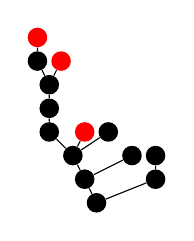
\begin{tikzpicture}[scale=.2]
\node[circle, scale=0.75, fill] (tid0) at (4.5,1.5){};
\node[circle, scale=0.75, fill] (tid1) at (3.75,3){};
\node[circle, scale=0.75, fill] (tid3) at (3,4.5){};
\node[circle, scale=0.75, fill] (tid6) at (1.5,6){};
\node[circle, scale=0.75, fill] (tid9) at (1.5,7.5){};
\node[circle, scale=0.75, fill] (tid10) at (1.5,9){};
\node[circle, scale=0.75, fill] (tid11) at (0.75,10.5){};
\node[circle, scale=0.75, fill, red] (tid13) at (0.75,12){};
\draw[](tid11) -- (tid13);
\node[circle, scale=0.75, fill, red] (tid12) at (2.25,10.5){};
\draw[](tid10) -- (tid11);
\draw[](tid10) -- (tid12);
\draw[](tid9) -- (tid10);
\draw[](tid6) -- (tid9);
\node[circle, scale=0.75, fill, red] (tid7) at (3.75,6){};
\node[circle, scale=0.75, fill] (tid8) at (5.25,6){};
\draw[](tid3) -- (tid6);
\draw[](tid3) -- (tid7);
\draw[](tid3) -- (tid8);
\node[circle, scale=0.75, fill] (tid4) at (6.75,4.5){};
\draw[](tid1) -- (tid3);
\draw[](tid1) -- (tid4);
\node[circle, scale=0.75, fill] (tid2) at (8.25,3){};
\node[circle, scale=0.75, fill] (tid5) at (8.25,4.5){};
\draw[](tid2) -- (tid5);
\draw[](tid0) -- (tid1);
\draw[](tid0) -- (tid2);
\end{tikzpicture}
\nodepart{two}
\footnotesize{31836439/3779136}
\nodepart{three}
\footnotesize{$100/3\:100/3\:100/3$}
};
 & 
\node[draw=black, rectangle split,  rectangle split parts=3] (sn0x71e010){
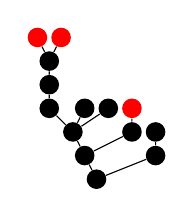
\begin{tikzpicture}[scale=.2]
\node[circle, scale=0.75, fill] (tid0) at (4.5,1.5){};
\node[circle, scale=0.75, fill] (tid1) at (3.75,3){};
\node[circle, scale=0.75, fill] (tid3) at (3,4.5){};
\node[circle, scale=0.75, fill] (tid6) at (1.5,6){};
\node[circle, scale=0.75, fill] (tid10) at (1.5,7.5){};
\node[circle, scale=0.75, fill] (tid11) at (1.5,9){};
\node[circle, scale=0.75, fill, red] (tid12) at (0.75,10.5){};
\node[circle, scale=0.75, fill, red] (tid13) at (2.25,10.5){};
\draw[](tid11) -- (tid12);
\draw[](tid11) -- (tid13);
\draw[](tid10) -- (tid11);
\draw[](tid6) -- (tid10);
\node[circle, scale=0.75, fill] (tid7) at (3.75,6){};
\node[circle, scale=0.75, fill] (tid8) at (5.25,6){};
\draw[](tid3) -- (tid6);
\draw[](tid3) -- (tid7);
\draw[](tid3) -- (tid8);
\node[circle, scale=0.75, fill] (tid4) at (6.75,4.5){};
\node[circle, scale=0.75, fill, red] (tid9) at (6.75,6){};
\draw[](tid4) -- (tid9);
\draw[](tid1) -- (tid3);
\draw[](tid1) -- (tid4);
\node[circle, scale=0.75, fill] (tid2) at (8.25,3){};
\node[circle, scale=0.75, fill] (tid5) at (8.25,4.5){};
\draw[](tid2) -- (tid5);
\draw[](tid0) -- (tid1);
\draw[](tid0) -- (tid2);
\end{tikzpicture}
\nodepart{two}
\footnotesize{7440803/944784}
\nodepart{three}
\footnotesize{$200/3\:100/3$}
};
 & 
\node[draw=black, rectangle split,  rectangle split parts=3] (sn0x71f370){
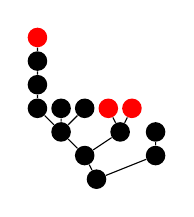
\begin{tikzpicture}[scale=.2]
\node[circle, scale=0.75, fill] (tid0) at (4.5,1.5){};
\node[circle, scale=0.75, fill] (tid1) at (3.75,3){};
\node[circle, scale=0.75, fill] (tid3) at (2.25,4.5){};
\node[circle, scale=0.75, fill] (tid6) at (0.75,6){};
\node[circle, scale=0.75, fill] (tid11) at (0.75,7.5){};
\node[circle, scale=0.75, fill] (tid12) at (0.75,9){};
\node[circle, scale=0.75, fill, red] (tid13) at (0.75,10.5){};
\draw[](tid12) -- (tid13);
\draw[](tid11) -- (tid12);
\draw[](tid6) -- (tid11);
\node[circle, scale=0.75, fill] (tid7) at (2.25,6){};
\node[circle, scale=0.75, fill] (tid8) at (3.75,6){};
\draw[](tid3) -- (tid6);
\draw[](tid3) -- (tid7);
\draw[](tid3) -- (tid8);
\node[circle, scale=0.75, fill] (tid4) at (6,4.5){};
\node[circle, scale=0.75, fill, red] (tid9) at (5.25,6){};
\node[circle, scale=0.75, fill, red] (tid10) at (6.75,6){};
\draw[](tid4) -- (tid9);
\draw[](tid4) -- (tid10);
\draw[](tid1) -- (tid3);
\draw[](tid1) -- (tid4);
\node[circle, scale=0.75, fill] (tid2) at (8.25,3){};
\node[circle, scale=0.75, fill] (tid5) at (8.25,4.5){};
\draw[](tid2) -- (tid5);
\draw[](tid0) -- (tid1);
\draw[](tid0) -- (tid2);
\end{tikzpicture}
\nodepart{two}
\footnotesize{28756963/3779136}
\nodepart{three}
\footnotesize{$200/3\:100/3$}
};
 & 
\node[draw=black, rectangle split,  rectangle split parts=3] (sn0x7228c0){
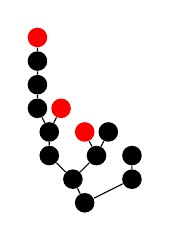
\begin{tikzpicture}[scale=.2]
\node[circle, scale=0.75, fill] (tid0) at (3.75,1.5){};
\node[circle, scale=0.75, fill] (tid1) at (3,3){};
\node[circle, scale=0.75, fill] (tid3) at (1.5,4.5){};
\node[circle, scale=0.75, fill] (tid6) at (1.5,6){};
\node[circle, scale=0.75, fill] (tid9) at (0.75,7.5){};
\node[circle, scale=0.75, fill] (tid11) at (0.75,9){};
\node[circle, scale=0.75, fill] (tid12) at (0.75,10.5){};
\node[circle, scale=0.75, fill, red] (tid13) at (0.75,12){};
\draw[](tid12) -- (tid13);
\draw[](tid11) -- (tid12);
\draw[](tid9) -- (tid11);
\node[circle, scale=0.75, fill, red] (tid10) at (2.25,7.5){};
\draw[](tid6) -- (tid9);
\draw[](tid6) -- (tid10);
\draw[](tid3) -- (tid6);
\node[circle, scale=0.75, fill] (tid4) at (4.5,4.5){};
\node[circle, scale=0.75, fill, red] (tid7) at (3.75,6){};
\node[circle, scale=0.75, fill] (tid8) at (5.25,6){};
\draw[](tid4) -- (tid7);
\draw[](tid4) -- (tid8);
\draw[](tid1) -- (tid3);
\draw[](tid1) -- (tid4);
\node[circle, scale=0.75, fill] (tid2) at (6.75,3){};
\node[circle, scale=0.75, fill] (tid5) at (6.75,4.5){};
\draw[](tid2) -- (tid5);
\draw[](tid0) -- (tid1);
\draw[](tid0) -- (tid2);
\end{tikzpicture}
\nodepart{two}
\footnotesize{27841889/3359232}
\nodepart{three}
\footnotesize{$100/3\:100/3\:100/3$}
};
 & 
\node[draw=black, rectangle split,  rectangle split parts=3] (sn0x71e5e0){
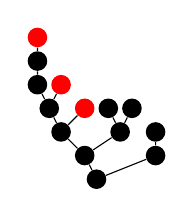
\begin{tikzpicture}[scale=.2]
\node[circle, scale=0.75, fill] (tid0) at (4.5,1.5){};
\node[circle, scale=0.75, fill] (tid1) at (3.75,3){};
\node[circle, scale=0.75, fill] (tid3) at (2.25,4.5){};
\node[circle, scale=0.75, fill] (tid6) at (1.5,6){};
\node[circle, scale=0.75, fill] (tid10) at (0.75,7.5){};
\node[circle, scale=0.75, fill] (tid12) at (0.75,9){};
\node[circle, scale=0.75, fill, red] (tid13) at (0.75,10.5){};
\draw[](tid12) -- (tid13);
\draw[](tid10) -- (tid12);
\node[circle, scale=0.75, fill, red] (tid11) at (2.25,7.5){};
\draw[](tid6) -- (tid10);
\draw[](tid6) -- (tid11);
\node[circle, scale=0.75, fill, red] (tid7) at (3.75,6){};
\draw[](tid3) -- (tid6);
\draw[](tid3) -- (tid7);
\node[circle, scale=0.75, fill] (tid4) at (6,4.5){};
\node[circle, scale=0.75, fill] (tid8) at (5.25,6){};
\node[circle, scale=0.75, fill] (tid9) at (6.75,6){};
\draw[](tid4) -- (tid8);
\draw[](tid4) -- (tid9);
\draw[](tid1) -- (tid3);
\draw[](tid1) -- (tid4);
\node[circle, scale=0.75, fill] (tid2) at (8.25,3){};
\node[circle, scale=0.75, fill] (tid5) at (8.25,4.5){};
\draw[](tid2) -- (tid5);
\draw[](tid0) -- (tid1);
\draw[](tid0) -- (tid2);
\end{tikzpicture}
\nodepart{two}
\footnotesize{28890049/3779136}
\nodepart{three}
\footnotesize{$100/3\:100/3\:100/3$}
};
 & 
\node[draw=black, rectangle split,  rectangle split parts=3] (sn0x734640){
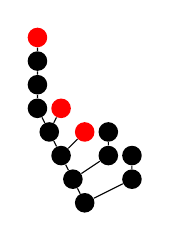
\begin{tikzpicture}[scale=.2]
\node[circle, scale=0.75, fill] (tid0) at (3.75,1.5){};
\node[circle, scale=0.75, fill] (tid1) at (3,3){};
\node[circle, scale=0.75, fill] (tid3) at (2.25,4.5){};
\node[circle, scale=0.75, fill] (tid6) at (1.5,6){};
\node[circle, scale=0.75, fill] (tid9) at (0.75,7.5){};
\node[circle, scale=0.75, fill] (tid11) at (0.75,9){};
\node[circle, scale=0.75, fill] (tid12) at (0.75,10.5){};
\node[circle, scale=0.75, fill, red] (tid13) at (0.75,12){};
\draw[](tid12) -- (tid13);
\draw[](tid11) -- (tid12);
\draw[](tid9) -- (tid11);
\node[circle, scale=0.75, fill, red] (tid10) at (2.25,7.5){};
\draw[](tid6) -- (tid9);
\draw[](tid6) -- (tid10);
\node[circle, scale=0.75, fill, red] (tid7) at (3.75,6){};
\draw[](tid3) -- (tid6);
\draw[](tid3) -- (tid7);
\node[circle, scale=0.75, fill] (tid4) at (5.25,4.5){};
\node[circle, scale=0.75, fill] (tid8) at (5.25,6){};
\draw[](tid4) -- (tid8);
\draw[](tid1) -- (tid3);
\draw[](tid1) -- (tid4);
\node[circle, scale=0.75, fill] (tid2) at (6.75,3){};
\node[circle, scale=0.75, fill] (tid5) at (6.75,4.5){};
\draw[](tid2) -- (tid5);
\draw[](tid0) -- (tid1);
\draw[](tid0) -- (tid2);
\end{tikzpicture}
\nodepart{two}
\footnotesize{125235245/15116544}
\nodepart{three}
\footnotesize{$100/3\:100/3\:100/3$}
};
 & 
\node[draw=black, rectangle split,  rectangle split parts=3] (sn0x736520){
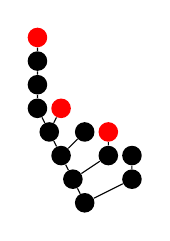
\begin{tikzpicture}[scale=.2]
\node[circle, scale=0.75, fill] (tid0) at (3.75,1.5){};
\node[circle, scale=0.75, fill] (tid1) at (3,3){};
\node[circle, scale=0.75, fill] (tid3) at (2.25,4.5){};
\node[circle, scale=0.75, fill] (tid6) at (1.5,6){};
\node[circle, scale=0.75, fill] (tid9) at (0.75,7.5){};
\node[circle, scale=0.75, fill] (tid11) at (0.75,9){};
\node[circle, scale=0.75, fill] (tid12) at (0.75,10.5){};
\node[circle, scale=0.75, fill, red] (tid13) at (0.75,12){};
\draw[](tid12) -- (tid13);
\draw[](tid11) -- (tid12);
\draw[](tid9) -- (tid11);
\node[circle, scale=0.75, fill, red] (tid10) at (2.25,7.5){};
\draw[](tid6) -- (tid9);
\draw[](tid6) -- (tid10);
\node[circle, scale=0.75, fill] (tid7) at (3.75,6){};
\draw[](tid3) -- (tid6);
\draw[](tid3) -- (tid7);
\node[circle, scale=0.75, fill] (tid4) at (5.25,4.5){};
\node[circle, scale=0.75, fill, red] (tid8) at (5.25,6){};
\draw[](tid4) -- (tid8);
\draw[](tid1) -- (tid3);
\draw[](tid1) -- (tid4);
\node[circle, scale=0.75, fill] (tid2) at (6.75,3){};
\node[circle, scale=0.75, fill] (tid5) at (6.75,4.5){};
\draw[](tid2) -- (tid5);
\draw[](tid0) -- (tid1);
\draw[](tid0) -- (tid2);
\end{tikzpicture}
\nodepart{two}
\footnotesize{250357595/30233088}
\nodepart{three}
\footnotesize{$100/3\:100/3\:100/3$}
};
 & 
\node[draw=black, rectangle split,  rectangle split parts=3] (sn0x739480){
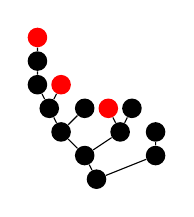
\begin{tikzpicture}[scale=.2]
\node[circle, scale=0.75, fill] (tid0) at (4.5,1.5){};
\node[circle, scale=0.75, fill] (tid1) at (3.75,3){};
\node[circle, scale=0.75, fill] (tid3) at (2.25,4.5){};
\node[circle, scale=0.75, fill] (tid6) at (1.5,6){};
\node[circle, scale=0.75, fill] (tid10) at (0.75,7.5){};
\node[circle, scale=0.75, fill] (tid12) at (0.75,9){};
\node[circle, scale=0.75, fill, red] (tid13) at (0.75,10.5){};
\draw[](tid12) -- (tid13);
\draw[](tid10) -- (tid12);
\node[circle, scale=0.75, fill, red] (tid11) at (2.25,7.5){};
\draw[](tid6) -- (tid10);
\draw[](tid6) -- (tid11);
\node[circle, scale=0.75, fill] (tid7) at (3.75,6){};
\draw[](tid3) -- (tid6);
\draw[](tid3) -- (tid7);
\node[circle, scale=0.75, fill] (tid4) at (6,4.5){};
\node[circle, scale=0.75, fill, red] (tid8) at (5.25,6){};
\node[circle, scale=0.75, fill] (tid9) at (6.75,6){};
\draw[](tid4) -- (tid8);
\draw[](tid4) -- (tid9);
\draw[](tid1) -- (tid3);
\draw[](tid1) -- (tid4);
\node[circle, scale=0.75, fill] (tid2) at (8.25,3){};
\node[circle, scale=0.75, fill] (tid5) at (8.25,4.5){};
\draw[](tid2) -- (tid5);
\draw[](tid0) -- (tid1);
\draw[](tid0) -- (tid2);
\end{tikzpicture}
\nodepart{two}
\footnotesize{28875485/3779136}
\nodepart{three}
\footnotesize{$50/3\:50/3\:50/3\:50/3\:100/3$}
};
 & 
\node[draw=black, rectangle split,  rectangle split parts=3] (sn0x740d10){
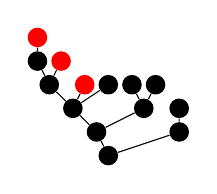
\begin{tikzpicture}[scale=.2]
\node[circle, scale=0.75, fill] (tid0) at (5.25,1.5){};
\node[circle, scale=0.75, fill] (tid1) at (4.5,3){};
\node[circle, scale=0.75, fill] (tid3) at (3,4.5){};
\node[circle, scale=0.75, fill] (tid6) at (1.5,6){};
\node[circle, scale=0.75, fill] (tid11) at (0.75,7.5){};
\node[circle, scale=0.75, fill, red] (tid13) at (0.75,9){};
\draw[](tid11) -- (tid13);
\node[circle, scale=0.75, fill, red] (tid12) at (2.25,7.5){};
\draw[](tid6) -- (tid11);
\draw[](tid6) -- (tid12);
\node[circle, scale=0.75, fill, red] (tid7) at (3.75,6){};
\node[circle, scale=0.75, fill] (tid8) at (5.25,6){};
\draw[](tid3) -- (tid6);
\draw[](tid3) -- (tid7);
\draw[](tid3) -- (tid8);
\node[circle, scale=0.75, fill] (tid4) at (7.5,4.5){};
\node[circle, scale=0.75, fill] (tid9) at (6.75,6){};
\node[circle, scale=0.75, fill] (tid10) at (8.25,6){};
\draw[](tid4) -- (tid9);
\draw[](tid4) -- (tid10);
\draw[](tid1) -- (tid3);
\draw[](tid1) -- (tid4);
\node[circle, scale=0.75, fill] (tid2) at (9.75,3){};
\node[circle, scale=0.75, fill] (tid5) at (9.75,4.5){};
\draw[](tid2) -- (tid5);
\draw[](tid0) -- (tid1);
\draw[](tid0) -- (tid2);
\end{tikzpicture}
\nodepart{two}
\footnotesize{13690285/1889568}
\nodepart{three}
\footnotesize{$100/9\:200/9\:100/9\:200/9\:100/3$}
};
 & 
\node[draw=black, rectangle split,  rectangle split parts=3] (sn0x73df60){
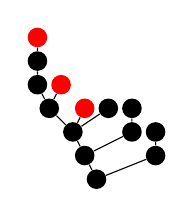
\begin{tikzpicture}[scale=.2]
\node[circle, scale=0.75, fill] (tid0) at (4.5,1.5){};
\node[circle, scale=0.75, fill] (tid1) at (3.75,3){};
\node[circle, scale=0.75, fill] (tid3) at (3,4.5){};
\node[circle, scale=0.75, fill] (tid6) at (1.5,6){};
\node[circle, scale=0.75, fill] (tid10) at (0.75,7.5){};
\node[circle, scale=0.75, fill] (tid12) at (0.75,9){};
\node[circle, scale=0.75, fill, red] (tid13) at (0.75,10.5){};
\draw[](tid12) -- (tid13);
\draw[](tid10) -- (tid12);
\node[circle, scale=0.75, fill, red] (tid11) at (2.25,7.5){};
\draw[](tid6) -- (tid10);
\draw[](tid6) -- (tid11);
\node[circle, scale=0.75, fill, red] (tid7) at (3.75,6){};
\node[circle, scale=0.75, fill] (tid8) at (5.25,6){};
\draw[](tid3) -- (tid6);
\draw[](tid3) -- (tid7);
\draw[](tid3) -- (tid8);
\node[circle, scale=0.75, fill] (tid4) at (6.75,4.5){};
\node[circle, scale=0.75, fill] (tid9) at (6.75,6){};
\draw[](tid4) -- (tid9);
\draw[](tid1) -- (tid3);
\draw[](tid1) -- (tid4);
\node[circle, scale=0.75, fill] (tid2) at (8.25,3){};
\node[circle, scale=0.75, fill] (tid5) at (8.25,4.5){};
\draw[](tid2) -- (tid5);
\draw[](tid0) -- (tid1);
\draw[](tid0) -- (tid2);
\end{tikzpicture}
\nodepart{two}
\footnotesize{57736459/7558272}
\nodepart{three}
\footnotesize{$50/3\:50/3\:50/3\:50/3\:100/3$}
};
 & 
\node[draw=black, rectangle split,  rectangle split parts=3] (sn0x744160){
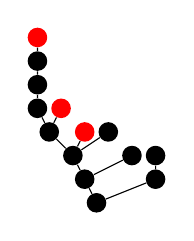
\begin{tikzpicture}[scale=.2]
\node[circle, scale=0.75, fill] (tid0) at (4.5,1.5){};
\node[circle, scale=0.75, fill] (tid1) at (3.75,3){};
\node[circle, scale=0.75, fill] (tid3) at (3,4.5){};
\node[circle, scale=0.75, fill] (tid6) at (1.5,6){};
\node[circle, scale=0.75, fill] (tid9) at (0.75,7.5){};
\node[circle, scale=0.75, fill] (tid11) at (0.75,9){};
\node[circle, scale=0.75, fill] (tid12) at (0.75,10.5){};
\node[circle, scale=0.75, fill, red] (tid13) at (0.75,12){};
\draw[](tid12) -- (tid13);
\draw[](tid11) -- (tid12);
\draw[](tid9) -- (tid11);
\node[circle, scale=0.75, fill, red] (tid10) at (2.25,7.5){};
\draw[](tid6) -- (tid9);
\draw[](tid6) -- (tid10);
\node[circle, scale=0.75, fill, red] (tid7) at (3.75,6){};
\node[circle, scale=0.75, fill] (tid8) at (5.25,6){};
\draw[](tid3) -- (tid6);
\draw[](tid3) -- (tid7);
\draw[](tid3) -- (tid8);
\node[circle, scale=0.75, fill] (tid4) at (6.75,4.5){};
\draw[](tid1) -- (tid3);
\draw[](tid1) -- (tid4);
\node[circle, scale=0.75, fill] (tid2) at (8.25,3){};
\node[circle, scale=0.75, fill] (tid5) at (8.25,4.5){};
\draw[](tid2) -- (tid5);
\draw[](tid0) -- (tid1);
\draw[](tid0) -- (tid2);
\end{tikzpicture}
\nodepart{two}
\footnotesize{62561891/7558272}
\nodepart{three}
\footnotesize{$100/3\:100/3\:100/3$}
};
 & 
\node[draw=black, rectangle split,  rectangle split parts=3] (sn0x747510){
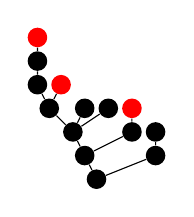
\begin{tikzpicture}[scale=.2]
\node[circle, scale=0.75, fill] (tid0) at (4.5,1.5){};
\node[circle, scale=0.75, fill] (tid1) at (3.75,3){};
\node[circle, scale=0.75, fill] (tid3) at (3,4.5){};
\node[circle, scale=0.75, fill] (tid6) at (1.5,6){};
\node[circle, scale=0.75, fill] (tid10) at (0.75,7.5){};
\node[circle, scale=0.75, fill] (tid12) at (0.75,9){};
\node[circle, scale=0.75, fill, red] (tid13) at (0.75,10.5){};
\draw[](tid12) -- (tid13);
\draw[](tid10) -- (tid12);
\node[circle, scale=0.75, fill, red] (tid11) at (2.25,7.5){};
\draw[](tid6) -- (tid10);
\draw[](tid6) -- (tid11);
\node[circle, scale=0.75, fill] (tid7) at (3.75,6){};
\node[circle, scale=0.75, fill] (tid8) at (5.25,6){};
\draw[](tid3) -- (tid6);
\draw[](tid3) -- (tid7);
\draw[](tid3) -- (tid8);
\node[circle, scale=0.75, fill] (tid4) at (6.75,4.5){};
\node[circle, scale=0.75, fill, red] (tid9) at (6.75,6){};
\draw[](tid4) -- (tid9);
\draw[](tid1) -- (tid3);
\draw[](tid1) -- (tid4);
\node[circle, scale=0.75, fill] (tid2) at (8.25,3){};
\node[circle, scale=0.75, fill] (tid5) at (8.25,4.5){};
\draw[](tid2) -- (tid5);
\draw[](tid0) -- (tid1);
\draw[](tid0) -- (tid2);
\end{tikzpicture}
\nodepart{two}
\footnotesize{19234985/2519424}
\nodepart{three}
\footnotesize{$100/3\:100/3\:100/3$}
};
 & 
\node[draw=black, rectangle split,  rectangle split parts=3] (sn0x74a800){
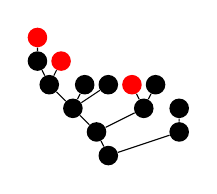
\begin{tikzpicture}[scale=.2]
\node[circle, scale=0.75, fill] (tid0) at (5.25,1.5){};
\node[circle, scale=0.75, fill] (tid1) at (4.5,3){};
\node[circle, scale=0.75, fill] (tid3) at (3,4.5){};
\node[circle, scale=0.75, fill] (tid6) at (1.5,6){};
\node[circle, scale=0.75, fill] (tid11) at (0.75,7.5){};
\node[circle, scale=0.75, fill, red] (tid13) at (0.75,9){};
\draw[](tid11) -- (tid13);
\node[circle, scale=0.75, fill, red] (tid12) at (2.25,7.5){};
\draw[](tid6) -- (tid11);
\draw[](tid6) -- (tid12);
\node[circle, scale=0.75, fill] (tid7) at (3.75,6){};
\node[circle, scale=0.75, fill] (tid8) at (5.25,6){};
\draw[](tid3) -- (tid6);
\draw[](tid3) -- (tid7);
\draw[](tid3) -- (tid8);
\node[circle, scale=0.75, fill] (tid4) at (7.5,4.5){};
\node[circle, scale=0.75, fill, red] (tid9) at (6.75,6){};
\node[circle, scale=0.75, fill] (tid10) at (8.25,6){};
\draw[](tid4) -- (tid9);
\draw[](tid4) -- (tid10);
\draw[](tid1) -- (tid3);
\draw[](tid1) -- (tid4);
\node[circle, scale=0.75, fill] (tid2) at (9.75,3){};
\node[circle, scale=0.75, fill] (tid5) at (9.75,4.5){};
\draw[](tid2) -- (tid5);
\draw[](tid0) -- (tid1);
\draw[](tid0) -- (tid2);
\end{tikzpicture}
\nodepart{two}
\footnotesize{164219609/22674816}
\nodepart{three}
\footnotesize{$200/9\:100/9\:200/9\:100/9\:100/3$}
};
 & 
\\
};
\end{scope}
\begin{scope}[yshift=\leveltopIIIII cm]
\matrix (line5) [column sep=1cm] {
\node[draw=black, rectangle split,  rectangle split parts=3] (sn0x6ccfb0){
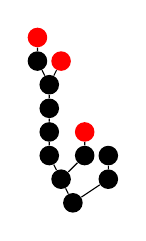
\begin{tikzpicture}[scale=.2]
\node[circle, scale=0.75, fill] (tid0) at (3,1.5){};
\node[circle, scale=0.75, fill] (tid1) at (2.25,3){};
\node[circle, scale=0.75, fill] (tid3) at (1.5,4.5){};
\node[circle, scale=0.75, fill] (tid6) at (1.5,6){};
\node[circle, scale=0.75, fill] (tid8) at (1.5,7.5){};
\node[circle, scale=0.75, fill] (tid9) at (1.5,9){};
\node[circle, scale=0.75, fill] (tid10) at (0.75,10.5){};
\node[circle, scale=0.75, fill, red] (tid12) at (0.75,12){};
\draw[](tid10) -- (tid12);
\node[circle, scale=0.75, fill, red] (tid11) at (2.25,10.5){};
\draw[](tid9) -- (tid10);
\draw[](tid9) -- (tid11);
\draw[](tid8) -- (tid9);
\draw[](tid6) -- (tid8);
\draw[](tid3) -- (tid6);
\node[circle, scale=0.75, fill] (tid4) at (3.75,4.5){};
\node[circle, scale=0.75, fill, red] (tid7) at (3.75,6){};
\draw[](tid4) -- (tid7);
\draw[](tid1) -- (tid3);
\draw[](tid1) -- (tid4);
\node[circle, scale=0.75, fill] (tid2) at (5.25,3){};
\node[circle, scale=0.75, fill] (tid5) at (5.25,4.5){};
\draw[](tid2) -- (tid5);
\draw[](tid0) -- (tid1);
\draw[](tid0) -- (tid2);
\end{tikzpicture}
\nodepart{two}
\footnotesize{84278365/10077696}
\nodepart{three}
\footnotesize{$50/3\:50/3\:100/3\:100/3$}
};
 & 
\node[draw=black, rectangle split,  rectangle split parts=3] (sn0x6ce1e0){
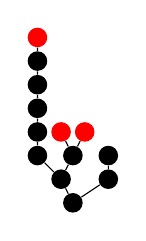
\begin{tikzpicture}[scale=.2]
\node[circle, scale=0.75, fill] (tid0) at (3,1.5){};
\node[circle, scale=0.75, fill] (tid1) at (2.25,3){};
\node[circle, scale=0.75, fill] (tid3) at (0.75,4.5){};
\node[circle, scale=0.75, fill] (tid6) at (0.75,6){};
\node[circle, scale=0.75, fill] (tid9) at (0.75,7.5){};
\node[circle, scale=0.75, fill] (tid10) at (0.75,9){};
\node[circle, scale=0.75, fill] (tid11) at (0.75,10.5){};
\node[circle, scale=0.75, fill, red] (tid12) at (0.75,12){};
\draw[](tid11) -- (tid12);
\draw[](tid10) -- (tid11);
\draw[](tid9) -- (tid10);
\draw[](tid6) -- (tid9);
\draw[](tid3) -- (tid6);
\node[circle, scale=0.75, fill] (tid4) at (3,4.5){};
\node[circle, scale=0.75, fill, red] (tid7) at (2.25,6){};
\node[circle, scale=0.75, fill, red] (tid8) at (3.75,6){};
\draw[](tid4) -- (tid7);
\draw[](tid4) -- (tid8);
\draw[](tid1) -- (tid3);
\draw[](tid1) -- (tid4);
\node[circle, scale=0.75, fill] (tid2) at (5.25,3){};
\node[circle, scale=0.75, fill] (tid5) at (5.25,4.5){};
\draw[](tid2) -- (tid5);
\draw[](tid0) -- (tid1);
\draw[](tid0) -- (tid2);
\end{tikzpicture}
\nodepart{two}
\footnotesize{6870833/839808}
\nodepart{three}
\footnotesize{$200/3\:100/3$}
};
 & 
\node[draw=black, rectangle split,  rectangle split parts=3] (sn0x6ced90){
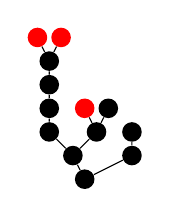
\begin{tikzpicture}[scale=.2]
\node[circle, scale=0.75, fill] (tid0) at (3.75,1.5){};
\node[circle, scale=0.75, fill] (tid1) at (3,3){};
\node[circle, scale=0.75, fill] (tid3) at (1.5,4.5){};
\node[circle, scale=0.75, fill] (tid6) at (1.5,6){};
\node[circle, scale=0.75, fill] (tid9) at (1.5,7.5){};
\node[circle, scale=0.75, fill] (tid10) at (1.5,9){};
\node[circle, scale=0.75, fill, red] (tid11) at (0.75,10.5){};
\node[circle, scale=0.75, fill, red] (tid12) at (2.25,10.5){};
\draw[](tid10) -- (tid11);
\draw[](tid10) -- (tid12);
\draw[](tid9) -- (tid10);
\draw[](tid6) -- (tid9);
\draw[](tid3) -- (tid6);
\node[circle, scale=0.75, fill] (tid4) at (4.5,4.5){};
\node[circle, scale=0.75, fill, red] (tid7) at (3.75,6){};
\node[circle, scale=0.75, fill] (tid8) at (5.25,6){};
\draw[](tid4) -- (tid7);
\draw[](tid4) -- (tid8);
\draw[](tid1) -- (tid3);
\draw[](tid1) -- (tid4);
\node[circle, scale=0.75, fill] (tid2) at (6.75,3){};
\node[circle, scale=0.75, fill] (tid5) at (6.75,4.5){};
\draw[](tid2) -- (tid5);
\draw[](tid0) -- (tid1);
\draw[](tid0) -- (tid2);
\end{tikzpicture}
\nodepart{two}
\footnotesize{1222469/157464}
\nodepart{three}
\footnotesize{$100/3\:200/3$}
};
 & 
\node[draw=black, rectangle split,  rectangle split parts=3] (sn0x6f07e0){
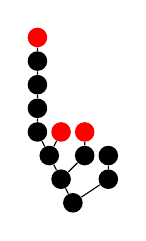
\begin{tikzpicture}[scale=.2]
\node[circle, scale=0.75, fill] (tid0) at (3,1.5){};
\node[circle, scale=0.75, fill] (tid1) at (2.25,3){};
\node[circle, scale=0.75, fill] (tid3) at (1.5,4.5){};
\node[circle, scale=0.75, fill] (tid6) at (0.75,6){};
\node[circle, scale=0.75, fill] (tid9) at (0.75,7.5){};
\node[circle, scale=0.75, fill] (tid10) at (0.75,9){};
\node[circle, scale=0.75, fill] (tid11) at (0.75,10.5){};
\node[circle, scale=0.75, fill, red] (tid12) at (0.75,12){};
\draw[](tid11) -- (tid12);
\draw[](tid10) -- (tid11);
\draw[](tid9) -- (tid10);
\draw[](tid6) -- (tid9);
\node[circle, scale=0.75, fill, red] (tid7) at (2.25,6){};
\draw[](tid3) -- (tid6);
\draw[](tid3) -- (tid7);
\node[circle, scale=0.75, fill] (tid4) at (3.75,4.5){};
\node[circle, scale=0.75, fill, red] (tid8) at (3.75,6){};
\draw[](tid4) -- (tid8);
\draw[](tid1) -- (tid3);
\draw[](tid1) -- (tid4);
\node[circle, scale=0.75, fill] (tid2) at (5.25,3){};
\node[circle, scale=0.75, fill] (tid5) at (5.25,4.5){};
\draw[](tid2) -- (tid5);
\draw[](tid0) -- (tid1);
\draw[](tid0) -- (tid2);
\end{tikzpicture}
\nodepart{two}
\footnotesize{27461207/3359232}
\nodepart{three}
\footnotesize{$100/3\:50/3\:50/3\:100/3$}
};
 & 
\node[draw=black, rectangle split,  rectangle split parts=3] (sn0x6f3200){
\begin{tikzpicture}[scale=.2]
\node[circle, scale=0.75, fill] (tid0) at (3.75,1.5){};
\node[circle, scale=0.75, fill] (tid1) at (3,3){};
\node[circle, scale=0.75, fill] (tid3) at (1.5,4.5){};
\node[circle, scale=0.75, fill] (tid6) at (0.75,6){};
\node[circle, scale=0.75, fill] (tid10) at (0.75,7.5){};
\node[circle, scale=0.75, fill] (tid11) at (0.75,9){};
\node[circle, scale=0.75, fill, red] (tid12) at (0.75,10.5){};
\draw[](tid11) -- (tid12);
\draw[](tid10) -- (tid11);
\draw[](tid6) -- (tid10);
\node[circle, scale=0.75, fill, red] (tid7) at (2.25,6){};
\draw[](tid3) -- (tid6);
\draw[](tid3) -- (tid7);
\node[circle, scale=0.75, fill] (tid4) at (4.5,4.5){};
\node[circle, scale=0.75, fill, red] (tid8) at (3.75,6){};
\node[circle, scale=0.75, fill] (tid9) at (5.25,6){};
\draw[](tid4) -- (tid8);
\draw[](tid4) -- (tid9);
\draw[](tid1) -- (tid3);
\draw[](tid1) -- (tid4);
\node[circle, scale=0.75, fill] (tid2) at (6.75,3){};
\node[circle, scale=0.75, fill] (tid5) at (6.75,4.5){};
\draw[](tid2) -- (tid5);
\draw[](tid0) -- (tid1);
\draw[](tid0) -- (tid2);
\end{tikzpicture}
\nodepart{two}
\footnotesize{3126911/419904}
\nodepart{three}
\footnotesize{$100/3\:100/3\:100/3$}
};
 & 
\node[draw=black, rectangle split,  rectangle split parts=3] (sn0x701f90){
\begin{tikzpicture}[scale=.2]
\node[circle, scale=0.75, fill] (tid0) at (3.75,1.5){};
\node[circle, scale=0.75, fill] (tid1) at (3,3){};
\node[circle, scale=0.75, fill] (tid3) at (2.25,4.5){};
\node[circle, scale=0.75, fill] (tid6) at (1.5,6){};
\node[circle, scale=0.75, fill] (tid9) at (1.5,7.5){};
\node[circle, scale=0.75, fill] (tid10) at (1.5,9){};
\node[circle, scale=0.75, fill, red] (tid11) at (0.75,10.5){};
\node[circle, scale=0.75, fill, red] (tid12) at (2.25,10.5){};
\draw[](tid10) -- (tid11);
\draw[](tid10) -- (tid12);
\draw[](tid9) -- (tid10);
\draw[](tid6) -- (tid9);
\node[circle, scale=0.75, fill, red] (tid7) at (3.75,6){};
\draw[](tid3) -- (tid6);
\draw[](tid3) -- (tid7);
\node[circle, scale=0.75, fill] (tid4) at (5.25,4.5){};
\node[circle, scale=0.75, fill] (tid8) at (5.25,6){};
\draw[](tid4) -- (tid8);
\draw[](tid1) -- (tid3);
\draw[](tid1) -- (tid4);
\node[circle, scale=0.75, fill] (tid2) at (6.75,3){};
\node[circle, scale=0.75, fill] (tid5) at (6.75,4.5){};
\draw[](tid2) -- (tid5);
\draw[](tid0) -- (tid1);
\draw[](tid0) -- (tid2);
\end{tikzpicture}
\nodepart{two}
\footnotesize{9773051/1259712}
\nodepart{three}
\footnotesize{$100/3\:200/3$}
};
 & 
\node[draw=black, rectangle split,  rectangle split parts=3] (sn0x705bf0){
\begin{tikzpicture}[scale=.2]
\node[circle, scale=0.75, fill] (tid0) at (3.75,1.5){};
\node[circle, scale=0.75, fill] (tid1) at (3,3){};
\node[circle, scale=0.75, fill] (tid3) at (2.25,4.5){};
\node[circle, scale=0.75, fill] (tid6) at (1.5,6){};
\node[circle, scale=0.75, fill] (tid8) at (1.5,7.5){};
\node[circle, scale=0.75, fill] (tid9) at (1.5,9){};
\node[circle, scale=0.75, fill] (tid10) at (0.75,10.5){};
\node[circle, scale=0.75, fill, red] (tid12) at (0.75,12){};
\draw[](tid10) -- (tid12);
\node[circle, scale=0.75, fill, red] (tid11) at (2.25,10.5){};
\draw[](tid9) -- (tid10);
\draw[](tid9) -- (tid11);
\draw[](tid8) -- (tid9);
\draw[](tid6) -- (tid8);
\node[circle, scale=0.75, fill, red] (tid7) at (3.75,6){};
\draw[](tid3) -- (tid6);
\draw[](tid3) -- (tid7);
\node[circle, scale=0.75, fill] (tid4) at (5.25,4.5){};
\draw[](tid1) -- (tid3);
\draw[](tid1) -- (tid4);
\node[circle, scale=0.75, fill] (tid2) at (6.75,3){};
\node[circle, scale=0.75, fill] (tid5) at (6.75,4.5){};
\draw[](tid2) -- (tid5);
\draw[](tid0) -- (tid1);
\draw[](tid0) -- (tid2);
\end{tikzpicture}
\nodepart{two}
\footnotesize{42101669/5038848}
\nodepart{three}
\footnotesize{$50/3\:50/3\:50/3\:50/3\:100/3$}
};
 & 
\node[draw=black, rectangle split,  rectangle split parts=3] (sn0x707610){
\begin{tikzpicture}[scale=.2]
\node[circle, scale=0.75, fill] (tid0) at (3.75,1.5){};
\node[circle, scale=0.75, fill] (tid1) at (3,3){};
\node[circle, scale=0.75, fill] (tid3) at (2.25,4.5){};
\node[circle, scale=0.75, fill] (tid6) at (1.5,6){};
\node[circle, scale=0.75, fill] (tid9) at (1.5,7.5){};
\node[circle, scale=0.75, fill] (tid10) at (1.5,9){};
\node[circle, scale=0.75, fill, red] (tid11) at (0.75,10.5){};
\node[circle, scale=0.75, fill, red] (tid12) at (2.25,10.5){};
\draw[](tid10) -- (tid11);
\draw[](tid10) -- (tid12);
\draw[](tid9) -- (tid10);
\draw[](tid6) -- (tid9);
\node[circle, scale=0.75, fill] (tid7) at (3.75,6){};
\draw[](tid3) -- (tid6);
\draw[](tid3) -- (tid7);
\node[circle, scale=0.75, fill] (tid4) at (5.25,4.5){};
\node[circle, scale=0.75, fill, red] (tid8) at (5.25,6){};
\draw[](tid4) -- (tid8);
\draw[](tid1) -- (tid3);
\draw[](tid1) -- (tid4);
\node[circle, scale=0.75, fill] (tid2) at (6.75,3){};
\node[circle, scale=0.75, fill] (tid5) at (6.75,4.5){};
\draw[](tid2) -- (tid5);
\draw[](tid0) -- (tid1);
\draw[](tid0) -- (tid2);
\end{tikzpicture}
\nodepart{two}
\footnotesize{9768619/1259712}
\nodepart{three}
\footnotesize{$200/3\:100/3$}
};
 & 
\node[draw=black, rectangle split,  rectangle split parts=3] (sn0x708c00){
\begin{tikzpicture}[scale=.2]
\node[circle, scale=0.75, fill] (tid0) at (3.75,1.5){};
\node[circle, scale=0.75, fill] (tid1) at (3,3){};
\node[circle, scale=0.75, fill] (tid3) at (1.5,4.5){};
\node[circle, scale=0.75, fill] (tid6) at (0.75,6){};
\node[circle, scale=0.75, fill] (tid10) at (0.75,7.5){};
\node[circle, scale=0.75, fill] (tid11) at (0.75,9){};
\node[circle, scale=0.75, fill, red] (tid12) at (0.75,10.5){};
\draw[](tid11) -- (tid12);
\draw[](tid10) -- (tid11);
\draw[](tid6) -- (tid10);
\node[circle, scale=0.75, fill] (tid7) at (2.25,6){};
\draw[](tid3) -- (tid6);
\draw[](tid3) -- (tid7);
\node[circle, scale=0.75, fill] (tid4) at (4.5,4.5){};
\node[circle, scale=0.75, fill, red] (tid8) at (3.75,6){};
\node[circle, scale=0.75, fill, red] (tid9) at (5.25,6){};
\draw[](tid4) -- (tid8);
\draw[](tid4) -- (tid9);
\draw[](tid1) -- (tid3);
\draw[](tid1) -- (tid4);
\node[circle, scale=0.75, fill] (tid2) at (6.75,3){};
\node[circle, scale=0.75, fill] (tid5) at (6.75,4.5){};
\draw[](tid2) -- (tid5);
\draw[](tid0) -- (tid1);
\draw[](tid0) -- (tid2);
\end{tikzpicture}
\nodepart{two}
\footnotesize{4687991/629856}
\nodepart{three}
\footnotesize{$200/3\:100/3$}
};
 & 
\node[draw=black, rectangle split,  rectangle split parts=3] (sn0x70b6b0){
\begin{tikzpicture}[scale=.2]
\node[circle, scale=0.75, fill] (tid0) at (4.5,1.5){};
\node[circle, scale=0.75, fill] (tid1) at (3.75,3){};
\node[circle, scale=0.75, fill] (tid3) at (2.25,4.5){};
\node[circle, scale=0.75, fill] (tid6) at (0.75,6){};
\node[circle, scale=0.75, fill] (tid11) at (0.75,7.5){};
\node[circle, scale=0.75, fill, red] (tid12) at (0.75,9){};
\draw[](tid11) -- (tid12);
\draw[](tid6) -- (tid11);
\node[circle, scale=0.75, fill, red] (tid7) at (2.25,6){};
\node[circle, scale=0.75, fill, red] (tid8) at (3.75,6){};
\draw[](tid3) -- (tid6);
\draw[](tid3) -- (tid7);
\draw[](tid3) -- (tid8);
\node[circle, scale=0.75, fill] (tid4) at (6,4.5){};
\node[circle, scale=0.75, fill] (tid9) at (5.25,6){};
\node[circle, scale=0.75, fill] (tid10) at (6.75,6){};
\draw[](tid4) -- (tid9);
\draw[](tid4) -- (tid10);
\draw[](tid1) -- (tid3);
\draw[](tid1) -- (tid4);
\node[circle, scale=0.75, fill] (tid2) at (8.25,3){};
\node[circle, scale=0.75, fill] (tid5) at (8.25,4.5){};
\draw[](tid2) -- (tid5);
\draw[](tid0) -- (tid1);
\draw[](tid0) -- (tid2);
\end{tikzpicture}
\nodepart{two}
\footnotesize{26289557/3779136}
\nodepart{three}
\footnotesize{$200/3\:100/3$}
};
 & 
\node[draw=black, rectangle split,  rectangle split parts=3] (sn0x7117f0){
\begin{tikzpicture}[scale=.2]
\node[circle, scale=0.75, fill] (tid0) at (3.75,1.5){};
\node[circle, scale=0.75, fill] (tid1) at (3,3){};
\node[circle, scale=0.75, fill] (tid3) at (2.25,4.5){};
\node[circle, scale=0.75, fill] (tid6) at (0.75,6){};
\node[circle, scale=0.75, fill] (tid10) at (0.75,7.5){};
\node[circle, scale=0.75, fill] (tid11) at (0.75,9){};
\node[circle, scale=0.75, fill, red] (tid12) at (0.75,10.5){};
\draw[](tid11) -- (tid12);
\draw[](tid10) -- (tid11);
\draw[](tid6) -- (tid10);
\node[circle, scale=0.75, fill, red] (tid7) at (2.25,6){};
\node[circle, scale=0.75, fill, red] (tid8) at (3.75,6){};
\draw[](tid3) -- (tid6);
\draw[](tid3) -- (tid7);
\draw[](tid3) -- (tid8);
\node[circle, scale=0.75, fill] (tid4) at (5.25,4.5){};
\node[circle, scale=0.75, fill] (tid9) at (5.25,6){};
\draw[](tid4) -- (tid9);
\draw[](tid1) -- (tid3);
\draw[](tid1) -- (tid4);
\node[circle, scale=0.75, fill] (tid2) at (6.75,3){};
\node[circle, scale=0.75, fill] (tid5) at (6.75,4.5){};
\draw[](tid2) -- (tid5);
\draw[](tid0) -- (tid1);
\draw[](tid0) -- (tid2);
\end{tikzpicture}
\nodepart{two}
\footnotesize{4687969/629856}
\nodepart{three}
\footnotesize{$200/3\:100/3$}
};
 & 
\node[draw=black, rectangle split,  rectangle split parts=3] (sn0x70ecd0){
\begin{tikzpicture}[scale=.2]
\node[circle, scale=0.75, fill] (tid0) at (3.75,1.5){};
\node[circle, scale=0.75, fill] (tid1) at (3,3){};
\node[circle, scale=0.75, fill] (tid3) at (2.25,4.5){};
\node[circle, scale=0.75, fill] (tid6) at (0.75,6){};
\node[circle, scale=0.75, fill] (tid9) at (0.75,7.5){};
\node[circle, scale=0.75, fill] (tid10) at (0.75,9){};
\node[circle, scale=0.75, fill] (tid11) at (0.75,10.5){};
\node[circle, scale=0.75, fill, red] (tid12) at (0.75,12){};
\draw[](tid11) -- (tid12);
\draw[](tid10) -- (tid11);
\draw[](tid9) -- (tid10);
\draw[](tid6) -- (tid9);
\node[circle, scale=0.75, fill, red] (tid7) at (2.25,6){};
\node[circle, scale=0.75, fill, red] (tid8) at (3.75,6){};
\draw[](tid3) -- (tid6);
\draw[](tid3) -- (tid7);
\draw[](tid3) -- (tid8);
\node[circle, scale=0.75, fill] (tid4) at (5.25,4.5){};
\draw[](tid1) -- (tid3);
\draw[](tid1) -- (tid4);
\node[circle, scale=0.75, fill] (tid2) at (6.75,3){};
\node[circle, scale=0.75, fill] (tid5) at (6.75,4.5){};
\draw[](tid2) -- (tid5);
\draw[](tid0) -- (tid1);
\draw[](tid0) -- (tid2);
\end{tikzpicture}
\nodepart{two}
\footnotesize{41158271/5038848}
\nodepart{three}
\footnotesize{$100/3\:100/3\:100/3$}
};
 & 
\node[draw=black, rectangle split,  rectangle split parts=3] (sn0x7137b0){
\begin{tikzpicture}[scale=.2]
\node[circle, scale=0.75, fill] (tid0) at (3.75,1.5){};
\node[circle, scale=0.75, fill] (tid1) at (3,3){};
\node[circle, scale=0.75, fill] (tid3) at (2.25,4.5){};
\node[circle, scale=0.75, fill] (tid6) at (0.75,6){};
\node[circle, scale=0.75, fill] (tid10) at (0.75,7.5){};
\node[circle, scale=0.75, fill] (tid11) at (0.75,9){};
\node[circle, scale=0.75, fill, red] (tid12) at (0.75,10.5){};
\draw[](tid11) -- (tid12);
\draw[](tid10) -- (tid11);
\draw[](tid6) -- (tid10);
\node[circle, scale=0.75, fill, red] (tid7) at (2.25,6){};
\node[circle, scale=0.75, fill] (tid8) at (3.75,6){};
\draw[](tid3) -- (tid6);
\draw[](tid3) -- (tid7);
\draw[](tid3) -- (tid8);
\node[circle, scale=0.75, fill] (tid4) at (5.25,4.5){};
\node[circle, scale=0.75, fill, red] (tid9) at (5.25,6){};
\draw[](tid4) -- (tid9);
\draw[](tid1) -- (tid3);
\draw[](tid1) -- (tid4);
\node[circle, scale=0.75, fill] (tid2) at (6.75,3){};
\node[circle, scale=0.75, fill] (tid5) at (6.75,4.5){};
\draw[](tid2) -- (tid5);
\draw[](tid0) -- (tid1);
\draw[](tid0) -- (tid2);
\end{tikzpicture}
\nodepart{two}
\footnotesize{9370879/1259712}
\nodepart{three}
\footnotesize{$100/3\:100/3\:100/3$}
};
 & 
\node[draw=black, rectangle split,  rectangle split parts=3] (sn0x717170){
\begin{tikzpicture}[scale=.2]
\node[circle, scale=0.75, fill] (tid0) at (4.5,1.5){};
\node[circle, scale=0.75, fill] (tid1) at (3.75,3){};
\node[circle, scale=0.75, fill] (tid3) at (2.25,4.5){};
\node[circle, scale=0.75, fill] (tid6) at (0.75,6){};
\node[circle, scale=0.75, fill] (tid11) at (0.75,7.5){};
\node[circle, scale=0.75, fill, red] (tid12) at (0.75,9){};
\draw[](tid11) -- (tid12);
\draw[](tid6) -- (tid11);
\node[circle, scale=0.75, fill, red] (tid7) at (2.25,6){};
\node[circle, scale=0.75, fill] (tid8) at (3.75,6){};
\draw[](tid3) -- (tid6);
\draw[](tid3) -- (tid7);
\draw[](tid3) -- (tid8);
\node[circle, scale=0.75, fill] (tid4) at (6,4.5){};
\node[circle, scale=0.75, fill, red] (tid9) at (5.25,6){};
\node[circle, scale=0.75, fill] (tid10) at (6.75,6){};
\draw[](tid4) -- (tid9);
\draw[](tid4) -- (tid10);
\draw[](tid1) -- (tid3);
\draw[](tid1) -- (tid4);
\node[circle, scale=0.75, fill] (tid2) at (8.25,3){};
\node[circle, scale=0.75, fill] (tid5) at (8.25,4.5){};
\draw[](tid2) -- (tid5);
\draw[](tid0) -- (tid1);
\draw[](tid0) -- (tid2);
\end{tikzpicture}
\nodepart{two}
\footnotesize{4379765/629856}
\nodepart{three}
\footnotesize{$50/3\:50/3\:50/3\:50/3\:100/3$}
};
 & 
\node[draw=black, rectangle split,  rectangle split parts=3] (sn0x71e0e0){
\begin{tikzpicture}[scale=.2]
\node[circle, scale=0.75, fill] (tid0) at (4.5,1.5){};
\node[circle, scale=0.75, fill] (tid1) at (3.75,3){};
\node[circle, scale=0.75, fill] (tid3) at (3,4.5){};
\node[circle, scale=0.75, fill] (tid6) at (1.5,6){};
\node[circle, scale=0.75, fill] (tid9) at (1.5,7.5){};
\node[circle, scale=0.75, fill] (tid10) at (1.5,9){};
\node[circle, scale=0.75, fill, red] (tid11) at (0.75,10.5){};
\node[circle, scale=0.75, fill, red] (tid12) at (2.25,10.5){};
\draw[](tid10) -- (tid11);
\draw[](tid10) -- (tid12);
\draw[](tid9) -- (tid10);
\draw[](tid6) -- (tid9);
\node[circle, scale=0.75, fill, red] (tid7) at (3.75,6){};
\node[circle, scale=0.75, fill] (tid8) at (5.25,6){};
\draw[](tid3) -- (tid6);
\draw[](tid3) -- (tid7);
\draw[](tid3) -- (tid8);
\node[circle, scale=0.75, fill] (tid4) at (6.75,4.5){};
\draw[](tid1) -- (tid3);
\draw[](tid1) -- (tid4);
\node[circle, scale=0.75, fill] (tid2) at (8.25,3){};
\node[circle, scale=0.75, fill] (tid5) at (8.25,4.5){};
\draw[](tid2) -- (tid5);
\draw[](tid0) -- (tid1);
\draw[](tid0) -- (tid2);
\end{tikzpicture}
\nodepart{two}
\footnotesize{180773/23328}
\nodepart{three}
\footnotesize{$100/3\:200/3$}
};
 & 
\node[draw=black, rectangle split,  rectangle split parts=3] (sn0x720d50){
\begin{tikzpicture}[scale=.2]
\node[circle, scale=0.75, fill] (tid0) at (4.5,1.5){};
\node[circle, scale=0.75, fill] (tid1) at (3.75,3){};
\node[circle, scale=0.75, fill] (tid3) at (2.25,4.5){};
\node[circle, scale=0.75, fill] (tid6) at (0.75,6){};
\node[circle, scale=0.75, fill] (tid11) at (0.75,7.5){};
\node[circle, scale=0.75, fill, red] (tid12) at (0.75,9){};
\draw[](tid11) -- (tid12);
\draw[](tid6) -- (tid11);
\node[circle, scale=0.75, fill] (tid7) at (2.25,6){};
\node[circle, scale=0.75, fill] (tid8) at (3.75,6){};
\draw[](tid3) -- (tid6);
\draw[](tid3) -- (tid7);
\draw[](tid3) -- (tid8);
\node[circle, scale=0.75, fill] (tid4) at (6,4.5){};
\node[circle, scale=0.75, fill, red] (tid9) at (5.25,6){};
\node[circle, scale=0.75, fill, red] (tid10) at (6.75,6){};
\draw[](tid4) -- (tid9);
\draw[](tid4) -- (tid10);
\draw[](tid1) -- (tid3);
\draw[](tid1) -- (tid4);
\node[circle, scale=0.75, fill] (tid2) at (8.25,3){};
\node[circle, scale=0.75, fill] (tid5) at (8.25,4.5){};
\draw[](tid2) -- (tid5);
\draw[](tid0) -- (tid1);
\draw[](tid0) -- (tid2);
\end{tikzpicture}
\nodepart{two}
\footnotesize{8755493/1259712}
\nodepart{three}
\footnotesize{$200/3\:100/3$}
};
 & 
\node[draw=black, rectangle split,  rectangle split parts=3] (sn0x724e00){
\begin{tikzpicture}[scale=.2]
\node[circle, scale=0.75, fill] (tid0) at (3,1.5){};
\node[circle, scale=0.75, fill] (tid1) at (2.25,3){};
\node[circle, scale=0.75, fill] (tid3) at (1.5,4.5){};
\node[circle, scale=0.75, fill] (tid6) at (1.5,6){};
\node[circle, scale=0.75, fill] (tid8) at (0.75,7.5){};
\node[circle, scale=0.75, fill] (tid10) at (0.75,9){};
\node[circle, scale=0.75, fill] (tid11) at (0.75,10.5){};
\node[circle, scale=0.75, fill, red] (tid12) at (0.75,12){};
\draw[](tid11) -- (tid12);
\draw[](tid10) -- (tid11);
\draw[](tid8) -- (tid10);
\node[circle, scale=0.75, fill, red] (tid9) at (2.25,7.5){};
\draw[](tid6) -- (tid8);
\draw[](tid6) -- (tid9);
\draw[](tid3) -- (tid6);
\node[circle, scale=0.75, fill] (tid4) at (3.75,4.5){};
\node[circle, scale=0.75, fill, red] (tid7) at (3.75,6){};
\draw[](tid4) -- (tid7);
\draw[](tid1) -- (tid3);
\draw[](tid1) -- (tid4);
\node[circle, scale=0.75, fill] (tid2) at (5.25,3){};
\node[circle, scale=0.75, fill] (tid5) at (5.25,4.5){};
\draw[](tid2) -- (tid5);
\draw[](tid0) -- (tid1);
\draw[](tid0) -- (tid2);
\end{tikzpicture}
\nodepart{two}
\footnotesize{27543719/3359232}
\nodepart{three}
\footnotesize{$100/3\:50/3\:50/3\:100/3$}
};
 & 
\node[draw=black, rectangle split,  rectangle split parts=3] (sn0x724b10){
\begin{tikzpicture}[scale=.2]
\node[circle, scale=0.75, fill] (tid0) at (3.75,1.5){};
\node[circle, scale=0.75, fill] (tid1) at (3,3){};
\node[circle, scale=0.75, fill] (tid3) at (1.5,4.5){};
\node[circle, scale=0.75, fill] (tid6) at (1.5,6){};
\node[circle, scale=0.75, fill] (tid9) at (0.75,7.5){};
\node[circle, scale=0.75, fill] (tid11) at (0.75,9){};
\node[circle, scale=0.75, fill, red] (tid12) at (0.75,10.5){};
\draw[](tid11) -- (tid12);
\draw[](tid9) -- (tid11);
\node[circle, scale=0.75, fill, red] (tid10) at (2.25,7.5){};
\draw[](tid6) -- (tid9);
\draw[](tid6) -- (tid10);
\draw[](tid3) -- (tid6);
\node[circle, scale=0.75, fill] (tid4) at (4.5,4.5){};
\node[circle, scale=0.75, fill, red] (tid7) at (3.75,6){};
\node[circle, scale=0.75, fill] (tid8) at (5.25,6){};
\draw[](tid4) -- (tid7);
\draw[](tid4) -- (tid8);
\draw[](tid1) -- (tid3);
\draw[](tid1) -- (tid4);
\node[circle, scale=0.75, fill] (tid2) at (6.75,3){};
\node[circle, scale=0.75, fill] (tid5) at (6.75,4.5){};
\draw[](tid2) -- (tid5);
\draw[](tid0) -- (tid1);
\draw[](tid0) -- (tid2);
\end{tikzpicture}
\nodepart{two}
\footnotesize{3142423/419904}
\nodepart{three}
\footnotesize{$100/3\:100/3\:100/3$}
};
 & 
\node[draw=black, rectangle split,  rectangle split parts=3] (sn0x7352a0){
\begin{tikzpicture}[scale=.2]
\node[circle, scale=0.75, fill] (tid0) at (4.5,1.5){};
\node[circle, scale=0.75, fill] (tid1) at (3.75,3){};
\node[circle, scale=0.75, fill] (tid3) at (2.25,4.5){};
\node[circle, scale=0.75, fill] (tid6) at (1.5,6){};
\node[circle, scale=0.75, fill] (tid10) at (0.75,7.5){};
\node[circle, scale=0.75, fill, red] (tid12) at (0.75,9){};
\draw[](tid10) -- (tid12);
\node[circle, scale=0.75, fill, red] (tid11) at (2.25,7.5){};
\draw[](tid6) -- (tid10);
\draw[](tid6) -- (tid11);
\node[circle, scale=0.75, fill, red] (tid7) at (3.75,6){};
\draw[](tid3) -- (tid6);
\draw[](tid3) -- (tid7);
\node[circle, scale=0.75, fill] (tid4) at (6,4.5){};
\node[circle, scale=0.75, fill] (tid8) at (5.25,6){};
\node[circle, scale=0.75, fill] (tid9) at (6.75,6){};
\draw[](tid4) -- (tid8);
\draw[](tid4) -- (tid9);
\draw[](tid1) -- (tid3);
\draw[](tid1) -- (tid4);
\node[circle, scale=0.75, fill] (tid2) at (8.25,3){};
\node[circle, scale=0.75, fill] (tid5) at (8.25,4.5){};
\draw[](tid2) -- (tid5);
\draw[](tid0) -- (tid1);
\draw[](tid0) -- (tid2);
\end{tikzpicture}
\nodepart{two}
\footnotesize{8822335/1259712}
\nodepart{three}
\footnotesize{$100/3\:100/3\:100/3$}
};
 & 
\node[draw=black, rectangle split,  rectangle split parts=3] (sn0x739550){
\begin{tikzpicture}[scale=.2]
\node[circle, scale=0.75, fill] (tid0) at (3.75,1.5){};
\node[circle, scale=0.75, fill] (tid1) at (3,3){};
\node[circle, scale=0.75, fill] (tid3) at (2.25,4.5){};
\node[circle, scale=0.75, fill] (tid6) at (1.5,6){};
\node[circle, scale=0.75, fill] (tid9) at (0.75,7.5){};
\node[circle, scale=0.75, fill] (tid11) at (0.75,9){};
\node[circle, scale=0.75, fill, red] (tid12) at (0.75,10.5){};
\draw[](tid11) -- (tid12);
\draw[](tid9) -- (tid11);
\node[circle, scale=0.75, fill, red] (tid10) at (2.25,7.5){};
\draw[](tid6) -- (tid9);
\draw[](tid6) -- (tid10);
\node[circle, scale=0.75, fill, red] (tid7) at (3.75,6){};
\draw[](tid3) -- (tid6);
\draw[](tid3) -- (tid7);
\node[circle, scale=0.75, fill] (tid4) at (5.25,4.5){};
\node[circle, scale=0.75, fill] (tid8) at (5.25,6){};
\draw[](tid4) -- (tid8);
\draw[](tid1) -- (tid3);
\draw[](tid1) -- (tid4);
\node[circle, scale=0.75, fill] (tid2) at (6.75,3){};
\node[circle, scale=0.75, fill] (tid5) at (6.75,4.5){};
\draw[](tid2) -- (tid5);
\draw[](tid0) -- (tid1);
\draw[](tid0) -- (tid2);
\end{tikzpicture}
\nodepart{two}
\footnotesize{2355563/314928}
\nodepart{three}
\footnotesize{$100/3\:100/3\:100/3$}
};
 & 
\node[draw=black, rectangle split,  rectangle split parts=3] (sn0x73a1e0){
\begin{tikzpicture}[scale=.2]
\node[circle, scale=0.75, fill] (tid0) at (3.75,1.5){};
\node[circle, scale=0.75, fill] (tid1) at (3,3){};
\node[circle, scale=0.75, fill] (tid3) at (2.25,4.5){};
\node[circle, scale=0.75, fill] (tid6) at (1.5,6){};
\node[circle, scale=0.75, fill] (tid8) at (0.75,7.5){};
\node[circle, scale=0.75, fill] (tid10) at (0.75,9){};
\node[circle, scale=0.75, fill] (tid11) at (0.75,10.5){};
\node[circle, scale=0.75, fill, red] (tid12) at (0.75,12){};
\draw[](tid11) -- (tid12);
\draw[](tid10) -- (tid11);
\draw[](tid8) -- (tid10);
\node[circle, scale=0.75, fill, red] (tid9) at (2.25,7.5){};
\draw[](tid6) -- (tid8);
\draw[](tid6) -- (tid9);
\node[circle, scale=0.75, fill, red] (tid7) at (3.75,6){};
\draw[](tid3) -- (tid6);
\draw[](tid3) -- (tid7);
\node[circle, scale=0.75, fill] (tid4) at (5.25,4.5){};
\draw[](tid1) -- (tid3);
\draw[](tid1) -- (tid4);
\node[circle, scale=0.75, fill] (tid2) at (6.75,3){};
\node[circle, scale=0.75, fill] (tid5) at (6.75,4.5){};
\draw[](tid2) -- (tid5);
\draw[](tid0) -- (tid1);
\draw[](tid0) -- (tid2);
\end{tikzpicture}
\nodepart{two}
\footnotesize{41281327/5038848}
\nodepart{three}
\footnotesize{$50/3\:50/3\:50/3\:50/3\:100/3$}
};
 & 
\node[draw=black, rectangle split,  rectangle split parts=3] (sn0x73afd0){
\begin{tikzpicture}[scale=.2]
\node[circle, scale=0.75, fill] (tid0) at (3.75,1.5){};
\node[circle, scale=0.75, fill] (tid1) at (3,3){};
\node[circle, scale=0.75, fill] (tid3) at (2.25,4.5){};
\node[circle, scale=0.75, fill] (tid6) at (1.5,6){};
\node[circle, scale=0.75, fill] (tid9) at (0.75,7.5){};
\node[circle, scale=0.75, fill] (tid11) at (0.75,9){};
\node[circle, scale=0.75, fill, red] (tid12) at (0.75,10.5){};
\draw[](tid11) -- (tid12);
\draw[](tid9) -- (tid11);
\node[circle, scale=0.75, fill, red] (tid10) at (2.25,7.5){};
\draw[](tid6) -- (tid9);
\draw[](tid6) -- (tid10);
\node[circle, scale=0.75, fill] (tid7) at (3.75,6){};
\draw[](tid3) -- (tid6);
\draw[](tid3) -- (tid7);
\node[circle, scale=0.75, fill] (tid4) at (5.25,4.5){};
\node[circle, scale=0.75, fill, red] (tid8) at (5.25,6){};
\draw[](tid4) -- (tid8);
\draw[](tid1) -- (tid3);
\draw[](tid1) -- (tid4);
\node[circle, scale=0.75, fill] (tid2) at (6.75,3){};
\node[circle, scale=0.75, fill] (tid5) at (6.75,4.5){};
\draw[](tid2) -- (tid5);
\draw[](tid0) -- (tid1);
\draw[](tid0) -- (tid2);
\end{tikzpicture}
\nodepart{two}
\footnotesize{3138901/419904}
\nodepart{three}
\footnotesize{$100/3\:100/3\:100/3$}
};
 & 
\node[draw=black, rectangle split,  rectangle split parts=3] (sn0x73f880){
\begin{tikzpicture}[scale=.2]
\node[circle, scale=0.75, fill] (tid0) at (4.5,1.5){};
\node[circle, scale=0.75, fill] (tid1) at (3.75,3){};
\node[circle, scale=0.75, fill] (tid3) at (2.25,4.5){};
\node[circle, scale=0.75, fill] (tid6) at (1.5,6){};
\node[circle, scale=0.75, fill] (tid10) at (0.75,7.5){};
\node[circle, scale=0.75, fill, red] (tid12) at (0.75,9){};
\draw[](tid10) -- (tid12);
\node[circle, scale=0.75, fill, red] (tid11) at (2.25,7.5){};
\draw[](tid6) -- (tid10);
\draw[](tid6) -- (tid11);
\node[circle, scale=0.75, fill] (tid7) at (3.75,6){};
\draw[](tid3) -- (tid6);
\draw[](tid3) -- (tid7);
\node[circle, scale=0.75, fill] (tid4) at (6,4.5){};
\node[circle, scale=0.75, fill, red] (tid8) at (5.25,6){};
\node[circle, scale=0.75, fill] (tid9) at (6.75,6){};
\draw[](tid4) -- (tid8);
\draw[](tid4) -- (tid9);
\draw[](tid1) -- (tid3);
\draw[](tid1) -- (tid4);
\node[circle, scale=0.75, fill] (tid2) at (8.25,3){};
\node[circle, scale=0.75, fill] (tid5) at (8.25,4.5){};
\draw[](tid2) -- (tid5);
\draw[](tid0) -- (tid1);
\draw[](tid0) -- (tid2);
\end{tikzpicture}
\nodepart{two}
\footnotesize{4408969/629856}
\nodepart{three}
\footnotesize{$50/3\:50/3\:50/3\:50/3\:100/3$}
};
 & 
\node[draw=black, rectangle split,  rectangle split parts=3] (sn0x740140){
\begin{tikzpicture}[scale=.2]
\node[circle, scale=0.75, fill] (tid0) at (5.25,1.5){};
\node[circle, scale=0.75, fill] (tid1) at (4.5,3){};
\node[circle, scale=0.75, fill] (tid3) at (3,4.5){};
\node[circle, scale=0.75, fill] (tid6) at (1.5,6){};
\node[circle, scale=0.75, fill, red] (tid11) at (0.75,7.5){};
\node[circle, scale=0.75, fill, red] (tid12) at (2.25,7.5){};
\draw[](tid6) -- (tid11);
\draw[](tid6) -- (tid12);
\node[circle, scale=0.75, fill, red] (tid7) at (3.75,6){};
\node[circle, scale=0.75, fill] (tid8) at (5.25,6){};
\draw[](tid3) -- (tid6);
\draw[](tid3) -- (tid7);
\draw[](tid3) -- (tid8);
\node[circle, scale=0.75, fill] (tid4) at (7.5,4.5){};
\node[circle, scale=0.75, fill] (tid9) at (6.75,6){};
\node[circle, scale=0.75, fill] (tid10) at (8.25,6){};
\draw[](tid4) -- (tid9);
\draw[](tid4) -- (tid10);
\draw[](tid1) -- (tid3);
\draw[](tid1) -- (tid4);
\node[circle, scale=0.75, fill] (tid2) at (9.75,3){};
\node[circle, scale=0.75, fill] (tid5) at (9.75,4.5){};
\draw[](tid2) -- (tid5);
\draw[](tid0) -- (tid1);
\draw[](tid0) -- (tid2);
\end{tikzpicture}
\nodepart{two}
\footnotesize{4804147/708588}
\nodepart{three}
\footnotesize{$200/9\:400/9\:100/9\:200/9$}
};
 & 
\node[draw=black, rectangle split,  rectangle split parts=3] (sn0x7429b0){
\begin{tikzpicture}[scale=.2]
\node[circle, scale=0.75, fill] (tid0) at (4.5,1.5){};
\node[circle, scale=0.75, fill] (tid1) at (3.75,3){};
\node[circle, scale=0.75, fill] (tid3) at (3,4.5){};
\node[circle, scale=0.75, fill] (tid6) at (1.5,6){};
\node[circle, scale=0.75, fill] (tid10) at (0.75,7.5){};
\node[circle, scale=0.75, fill, red] (tid12) at (0.75,9){};
\draw[](tid10) -- (tid12);
\node[circle, scale=0.75, fill, red] (tid11) at (2.25,7.5){};
\draw[](tid6) -- (tid10);
\draw[](tid6) -- (tid11);
\node[circle, scale=0.75, fill, red] (tid7) at (3.75,6){};
\node[circle, scale=0.75, fill] (tid8) at (5.25,6){};
\draw[](tid3) -- (tid6);
\draw[](tid3) -- (tid7);
\draw[](tid3) -- (tid8);
\node[circle, scale=0.75, fill] (tid4) at (6.75,4.5){};
\node[circle, scale=0.75, fill] (tid9) at (6.75,6){};
\draw[](tid4) -- (tid9);
\draw[](tid1) -- (tid3);
\draw[](tid1) -- (tid4);
\node[circle, scale=0.75, fill] (tid2) at (8.25,3){};
\node[circle, scale=0.75, fill] (tid5) at (8.25,4.5){};
\draw[](tid2) -- (tid5);
\draw[](tid0) -- (tid1);
\draw[](tid0) -- (tid2);
\end{tikzpicture}
\nodepart{two}
\footnotesize{17631263/2519424}
\nodepart{three}
\footnotesize{$50/3\:50/3\:50/3\:50/3\:100/3$}
};
 & 
\node[draw=black, rectangle split,  rectangle split parts=3] (sn0x746d90){
\begin{tikzpicture}[scale=.2]
\node[circle, scale=0.75, fill] (tid0) at (4.5,1.5){};
\node[circle, scale=0.75, fill] (tid1) at (3.75,3){};
\node[circle, scale=0.75, fill] (tid3) at (3,4.5){};
\node[circle, scale=0.75, fill] (tid6) at (1.5,6){};
\node[circle, scale=0.75, fill] (tid9) at (0.75,7.5){};
\node[circle, scale=0.75, fill] (tid11) at (0.75,9){};
\node[circle, scale=0.75, fill, red] (tid12) at (0.75,10.5){};
\draw[](tid11) -- (tid12);
\draw[](tid9) -- (tid11);
\node[circle, scale=0.75, fill, red] (tid10) at (2.25,7.5){};
\draw[](tid6) -- (tid9);
\draw[](tid6) -- (tid10);
\node[circle, scale=0.75, fill, red] (tid7) at (3.75,6){};
\node[circle, scale=0.75, fill] (tid8) at (5.25,6){};
\draw[](tid3) -- (tid6);
\draw[](tid3) -- (tid7);
\draw[](tid3) -- (tid8);
\node[circle, scale=0.75, fill] (tid4) at (6.75,4.5){};
\draw[](tid1) -- (tid3);
\draw[](tid1) -- (tid4);
\node[circle, scale=0.75, fill] (tid2) at (8.25,3){};
\node[circle, scale=0.75, fill] (tid5) at (8.25,4.5){};
\draw[](tid2) -- (tid5);
\draw[](tid0) -- (tid1);
\draw[](tid0) -- (tid2);
\end{tikzpicture}
\nodepart{two}
\footnotesize{4705667/629856}
\nodepart{three}
\footnotesize{$100/3\:100/3\:100/3$}
};
 & 
\node[draw=black, rectangle split,  rectangle split parts=3] (sn0x74a540){
\begin{tikzpicture}[scale=.2]
\node[circle, scale=0.75, fill] (tid0) at (4.5,1.5){};
\node[circle, scale=0.75, fill] (tid1) at (3.75,3){};
\node[circle, scale=0.75, fill] (tid3) at (3,4.5){};
\node[circle, scale=0.75, fill] (tid6) at (1.5,6){};
\node[circle, scale=0.75, fill] (tid10) at (0.75,7.5){};
\node[circle, scale=0.75, fill, red] (tid12) at (0.75,9){};
\draw[](tid10) -- (tid12);
\node[circle, scale=0.75, fill, red] (tid11) at (2.25,7.5){};
\draw[](tid6) -- (tid10);
\draw[](tid6) -- (tid11);
\node[circle, scale=0.75, fill] (tid7) at (3.75,6){};
\node[circle, scale=0.75, fill] (tid8) at (5.25,6){};
\draw[](tid3) -- (tid6);
\draw[](tid3) -- (tid7);
\draw[](tid3) -- (tid8);
\node[circle, scale=0.75, fill] (tid4) at (6.75,4.5){};
\node[circle, scale=0.75, fill, red] (tid9) at (6.75,6){};
\draw[](tid4) -- (tid9);
\draw[](tid1) -- (tid3);
\draw[](tid1) -- (tid4);
\node[circle, scale=0.75, fill] (tid2) at (8.25,3){};
\node[circle, scale=0.75, fill] (tid5) at (8.25,4.5){};
\draw[](tid2) -- (tid5);
\draw[](tid0) -- (tid1);
\draw[](tid0) -- (tid2);
\end{tikzpicture}
\nodepart{two}
\footnotesize{17621105/2519424}
\nodepart{three}
\footnotesize{$100/3\:100/3\:100/3$}
};
 & 
\node[draw=black, rectangle split,  rectangle split parts=3] (sn0x743200){
\begin{tikzpicture}[scale=.2]
\node[circle, scale=0.75, fill] (tid0) at (5.25,1.5){};
\node[circle, scale=0.75, fill] (tid1) at (4.5,3){};
\node[circle, scale=0.75, fill] (tid3) at (3,4.5){};
\node[circle, scale=0.75, fill] (tid6) at (1.5,6){};
\node[circle, scale=0.75, fill, red] (tid11) at (0.75,7.5){};
\node[circle, scale=0.75, fill, red] (tid12) at (2.25,7.5){};
\draw[](tid6) -- (tid11);
\draw[](tid6) -- (tid12);
\node[circle, scale=0.75, fill] (tid7) at (3.75,6){};
\node[circle, scale=0.75, fill] (tid8) at (5.25,6){};
\draw[](tid3) -- (tid6);
\draw[](tid3) -- (tid7);
\draw[](tid3) -- (tid8);
\node[circle, scale=0.75, fill] (tid4) at (7.5,4.5){};
\node[circle, scale=0.75, fill, red] (tid9) at (6.75,6){};
\node[circle, scale=0.75, fill] (tid10) at (8.25,6){};
\draw[](tid4) -- (tid9);
\draw[](tid4) -- (tid10);
\draw[](tid1) -- (tid3);
\draw[](tid1) -- (tid4);
\node[circle, scale=0.75, fill] (tid2) at (9.75,3){};
\node[circle, scale=0.75, fill] (tid5) at (9.75,4.5){};
\draw[](tid2) -- (tid5);
\draw[](tid0) -- (tid1);
\draw[](tid0) -- (tid2);
\end{tikzpicture}
\nodepart{two}
\footnotesize{2134525/314928}
\nodepart{three}
\footnotesize{$400/9\:200/9\:200/9\:100/9$}
};
 & 
\\
};
\end{scope}
\begin{scope}[yshift=\leveltopIIIIII cm]
\matrix (line6) [column sep=1cm] {
\node[draw=black, rectangle split,  rectangle split parts=3] (sn0x6cd5b0){
\begin{tikzpicture}[scale=.2]
\node[circle, scale=0.75, fill] (tid0) at (3,1.5){};
\node[circle, scale=0.75, fill] (tid1) at (2.25,3){};
\node[circle, scale=0.75, fill] (tid3) at (1.5,4.5){};
\node[circle, scale=0.75, fill] (tid6) at (1.5,6){};
\node[circle, scale=0.75, fill] (tid7) at (1.5,7.5){};
\node[circle, scale=0.75, fill] (tid8) at (1.5,9){};
\node[circle, scale=0.75, fill] (tid9) at (0.75,10.5){};
\node[circle, scale=0.75, fill, red] (tid11) at (0.75,12){};
\draw[](tid9) -- (tid11);
\node[circle, scale=0.75, fill, red] (tid10) at (2.25,10.5){};
\draw[](tid8) -- (tid9);
\draw[](tid8) -- (tid10);
\draw[](tid7) -- (tid8);
\draw[](tid6) -- (tid7);
\draw[](tid3) -- (tid6);
\node[circle, scale=0.75, fill, red] (tid4) at (3.75,4.5){};
\draw[](tid1) -- (tid3);
\draw[](tid1) -- (tid4);
\node[circle, scale=0.75, fill] (tid2) at (5.25,3){};
\node[circle, scale=0.75, fill] (tid5) at (5.25,4.5){};
\draw[](tid2) -- (tid5);
\draw[](tid0) -- (tid1);
\draw[](tid0) -- (tid2);
\end{tikzpicture}
\nodepart{two}
\footnotesize{6979087/839808}
\nodepart{three}
\footnotesize{$100/3\:100/3\:100/3$}
};
 & 
\node[draw=black, rectangle split,  rectangle split parts=3] (sn0x6cd9a0){
\begin{tikzpicture}[scale=.2]
\node[circle, scale=0.75, fill] (tid0) at (3,1.5){};
\node[circle, scale=0.75, fill] (tid1) at (2.25,3){};
\node[circle, scale=0.75, fill] (tid3) at (1.5,4.5){};
\node[circle, scale=0.75, fill] (tid6) at (1.5,6){};
\node[circle, scale=0.75, fill] (tid7) at (1.5,7.5){};
\node[circle, scale=0.75, fill] (tid8) at (1.5,9){};
\node[circle, scale=0.75, fill] (tid9) at (0.75,10.5){};
\node[circle, scale=0.75, fill, red] (tid11) at (0.75,12){};
\draw[](tid9) -- (tid11);
\node[circle, scale=0.75, fill, red] (tid10) at (2.25,10.5){};
\draw[](tid8) -- (tid9);
\draw[](tid8) -- (tid10);
\draw[](tid7) -- (tid8);
\draw[](tid6) -- (tid7);
\draw[](tid3) -- (tid6);
\node[circle, scale=0.75, fill] (tid4) at (3.75,4.5){};
\draw[](tid1) -- (tid3);
\draw[](tid1) -- (tid4);
\node[circle, scale=0.75, fill] (tid2) at (5.25,3){};
\node[circle, scale=0.75, fill, red] (tid5) at (5.25,4.5){};
\draw[](tid2) -- (tid5);
\draw[](tid0) -- (tid1);
\draw[](tid0) -- (tid2);
\end{tikzpicture}
\nodepart{two}
\footnotesize{4648811/559872}
\nodepart{three}
\footnotesize{$100/3\:100/3\:100/3$}
};
 & 
\node[draw=black, rectangle split,  rectangle split parts=3] (sn0x6d0890){
\begin{tikzpicture}[scale=.2]
\node[circle, scale=0.75, fill] (tid0) at (2.25,1.5){};
\node[circle, scale=0.75, fill] (tid1) at (1.5,3){};
\node[circle, scale=0.75, fill] (tid3) at (0.75,4.5){};
\node[circle, scale=0.75, fill] (tid6) at (0.75,6){};
\node[circle, scale=0.75, fill] (tid8) at (0.75,7.5){};
\node[circle, scale=0.75, fill] (tid9) at (0.75,9){};
\node[circle, scale=0.75, fill] (tid10) at (0.75,10.5){};
\node[circle, scale=0.75, fill, red] (tid11) at (0.75,12){};
\draw[](tid10) -- (tid11);
\draw[](tid9) -- (tid10);
\draw[](tid8) -- (tid9);
\draw[](tid6) -- (tid8);
\draw[](tid3) -- (tid6);
\node[circle, scale=0.75, fill] (tid4) at (2.25,4.5){};
\node[circle, scale=0.75, fill, red] (tid7) at (2.25,6){};
\draw[](tid4) -- (tid7);
\draw[](tid1) -- (tid3);
\draw[](tid1) -- (tid4);
\node[circle, scale=0.75, fill] (tid2) at (3.75,3){};
\node[circle, scale=0.75, fill, red] (tid5) at (3.75,4.5){};
\draw[](tid2) -- (tid5);
\draw[](tid0) -- (tid1);
\draw[](tid0) -- (tid2);
\end{tikzpicture}
\nodepart{two}
\footnotesize{4543909/559872}
\nodepart{three}
\footnotesize{$100/3\:100/3\:100/3$}
};
 & 
\node[draw=black, rectangle split,  rectangle split parts=3] (sn0x6d0350){
\begin{tikzpicture}[scale=.2]
\node[circle, scale=0.75, fill] (tid0) at (3,1.5){};
\node[circle, scale=0.75, fill] (tid1) at (2.25,3){};
\node[circle, scale=0.75, fill] (tid3) at (1.5,4.5){};
\node[circle, scale=0.75, fill] (tid6) at (1.5,6){};
\node[circle, scale=0.75, fill] (tid8) at (1.5,7.5){};
\node[circle, scale=0.75, fill] (tid9) at (1.5,9){};
\node[circle, scale=0.75, fill, red] (tid10) at (0.75,10.5){};
\node[circle, scale=0.75, fill, red] (tid11) at (2.25,10.5){};
\draw[](tid9) -- (tid10);
\draw[](tid9) -- (tid11);
\draw[](tid8) -- (tid9);
\draw[](tid6) -- (tid8);
\draw[](tid3) -- (tid6);
\node[circle, scale=0.75, fill] (tid4) at (3.75,4.5){};
\node[circle, scale=0.75, fill, red] (tid7) at (3.75,6){};
\draw[](tid4) -- (tid7);
\draw[](tid1) -- (tid3);
\draw[](tid1) -- (tid4);
\node[circle, scale=0.75, fill] (tid2) at (5.25,3){};
\node[circle, scale=0.75, fill] (tid5) at (5.25,4.5){};
\draw[](tid2) -- (tid5);
\draw[](tid0) -- (tid1);
\draw[](tid0) -- (tid2);
\end{tikzpicture}
\nodepart{two}
\footnotesize{804721/104976}
\nodepart{three}
\footnotesize{$50/3\:50/3\:200/3$}
};
 & 
\node[draw=black, rectangle split,  rectangle split parts=3] (sn0x6eaf60){
\begin{tikzpicture}[scale=.2]
\node[circle, scale=0.75, fill] (tid0) at (3,1.5){};
\node[circle, scale=0.75, fill] (tid1) at (2.25,3){};
\node[circle, scale=0.75, fill] (tid3) at (0.75,4.5){};
\node[circle, scale=0.75, fill] (tid6) at (0.75,6){};
\node[circle, scale=0.75, fill] (tid9) at (0.75,7.5){};
\node[circle, scale=0.75, fill] (tid10) at (0.75,9){};
\node[circle, scale=0.75, fill, red] (tid11) at (0.75,10.5){};
\draw[](tid10) -- (tid11);
\draw[](tid9) -- (tid10);
\draw[](tid6) -- (tid9);
\draw[](tid3) -- (tid6);
\node[circle, scale=0.75, fill] (tid4) at (3,4.5){};
\node[circle, scale=0.75, fill, red] (tid7) at (2.25,6){};
\node[circle, scale=0.75, fill, red] (tid8) at (3.75,6){};
\draw[](tid4) -- (tid7);
\draw[](tid4) -- (tid8);
\draw[](tid1) -- (tid3);
\draw[](tid1) -- (tid4);
\node[circle, scale=0.75, fill] (tid2) at (5.25,3){};
\node[circle, scale=0.75, fill] (tid5) at (5.25,4.5){};
\draw[](tid2) -- (tid5);
\draw[](tid0) -- (tid1);
\draw[](tid0) -- (tid2);
\end{tikzpicture}
\nodepart{two}
\footnotesize{511747/69984}
\nodepart{three}
\footnotesize{$200/3\:100/3$}
};
 & 
\node[draw=black, rectangle split,  rectangle split parts=3] (sn0x6f1b20){
\begin{tikzpicture}[scale=.2]
\node[circle, scale=0.75, fill] (tid0) at (3,1.5){};
\node[circle, scale=0.75, fill] (tid1) at (2.25,3){};
\node[circle, scale=0.75, fill] (tid3) at (1.5,4.5){};
\node[circle, scale=0.75, fill] (tid6) at (0.75,6){};
\node[circle, scale=0.75, fill] (tid8) at (0.75,7.5){};
\node[circle, scale=0.75, fill] (tid9) at (0.75,9){};
\node[circle, scale=0.75, fill] (tid10) at (0.75,10.5){};
\node[circle, scale=0.75, fill, red] (tid11) at (0.75,12){};
\draw[](tid10) -- (tid11);
\draw[](tid9) -- (tid10);
\draw[](tid8) -- (tid9);
\draw[](tid6) -- (tid8);
\node[circle, scale=0.75, fill, red] (tid7) at (2.25,6){};
\draw[](tid3) -- (tid6);
\draw[](tid3) -- (tid7);
\node[circle, scale=0.75, fill, red] (tid4) at (3.75,4.5){};
\draw[](tid1) -- (tid3);
\draw[](tid1) -- (tid4);
\node[circle, scale=0.75, fill] (tid2) at (5.25,3){};
\node[circle, scale=0.75, fill] (tid5) at (5.25,4.5){};
\draw[](tid2) -- (tid5);
\draw[](tid0) -- (tid1);
\draw[](tid0) -- (tid2);
\end{tikzpicture}
\nodepart{two}
\footnotesize{6809695/839808}
\nodepart{three}
\footnotesize{$100/3\:100/3\:100/3$}
};
 & 
\node[draw=black, rectangle split,  rectangle split parts=3] (sn0x6f16c0){
\begin{tikzpicture}[scale=.2]
\node[circle, scale=0.75, fill] (tid0) at (3,1.5){};
\node[circle, scale=0.75, fill] (tid1) at (2.25,3){};
\node[circle, scale=0.75, fill] (tid3) at (1.5,4.5){};
\node[circle, scale=0.75, fill] (tid6) at (0.75,6){};
\node[circle, scale=0.75, fill] (tid8) at (0.75,7.5){};
\node[circle, scale=0.75, fill] (tid9) at (0.75,9){};
\node[circle, scale=0.75, fill] (tid10) at (0.75,10.5){};
\node[circle, scale=0.75, fill, red] (tid11) at (0.75,12){};
\draw[](tid10) -- (tid11);
\draw[](tid9) -- (tid10);
\draw[](tid8) -- (tid9);
\draw[](tid6) -- (tid8);
\node[circle, scale=0.75, fill, red] (tid7) at (2.25,6){};
\draw[](tid3) -- (tid6);
\draw[](tid3) -- (tid7);
\node[circle, scale=0.75, fill] (tid4) at (3.75,4.5){};
\draw[](tid1) -- (tid3);
\draw[](tid1) -- (tid4);
\node[circle, scale=0.75, fill] (tid2) at (5.25,3){};
\node[circle, scale=0.75, fill, red] (tid5) at (5.25,4.5){};
\draw[](tid2) -- (tid5);
\draw[](tid0) -- (tid1);
\draw[](tid0) -- (tid2);
\end{tikzpicture}
\nodepart{two}
\footnotesize{4534831/559872}
\nodepart{three}
\footnotesize{$100/3\:100/3\:100/3$}
};
 & 
\node[draw=black, rectangle split,  rectangle split parts=3] (sn0x6f1fa0){
\begin{tikzpicture}[scale=.2]
\node[circle, scale=0.75, fill] (tid0) at (3,1.5){};
\node[circle, scale=0.75, fill] (tid1) at (2.25,3){};
\node[circle, scale=0.75, fill] (tid3) at (1.5,4.5){};
\node[circle, scale=0.75, fill] (tid6) at (0.75,6){};
\node[circle, scale=0.75, fill] (tid9) at (0.75,7.5){};
\node[circle, scale=0.75, fill] (tid10) at (0.75,9){};
\node[circle, scale=0.75, fill, red] (tid11) at (0.75,10.5){};
\draw[](tid10) -- (tid11);
\draw[](tid9) -- (tid10);
\draw[](tid6) -- (tid9);
\node[circle, scale=0.75, fill, red] (tid7) at (2.25,6){};
\draw[](tid3) -- (tid6);
\draw[](tid3) -- (tid7);
\node[circle, scale=0.75, fill] (tid4) at (3.75,4.5){};
\node[circle, scale=0.75, fill, red] (tid8) at (3.75,6){};
\draw[](tid4) -- (tid8);
\draw[](tid1) -- (tid3);
\draw[](tid1) -- (tid4);
\node[circle, scale=0.75, fill] (tid2) at (5.25,3){};
\node[circle, scale=0.75, fill] (tid5) at (5.25,4.5){};
\draw[](tid2) -- (tid5);
\draw[](tid0) -- (tid1);
\draw[](tid0) -- (tid2);
\end{tikzpicture}
\nodepart{two}
\footnotesize{6134263/839808}
\nodepart{three}
\footnotesize{$100/3\:50/3\:50/3\:100/3$}
};
 & 
\node[draw=black, rectangle split,  rectangle split parts=3] (sn0x7012e0){
\begin{tikzpicture}[scale=.2]
\node[circle, scale=0.75, fill] (tid0) at (3.75,1.5){};
\node[circle, scale=0.75, fill] (tid1) at (3,3){};
\node[circle, scale=0.75, fill] (tid3) at (1.5,4.5){};
\node[circle, scale=0.75, fill] (tid6) at (0.75,6){};
\node[circle, scale=0.75, fill] (tid10) at (0.75,7.5){};
\node[circle, scale=0.75, fill, red] (tid11) at (0.75,9){};
\draw[](tid10) -- (tid11);
\draw[](tid6) -- (tid10);
\node[circle, scale=0.75, fill, red] (tid7) at (2.25,6){};
\draw[](tid3) -- (tid6);
\draw[](tid3) -- (tid7);
\node[circle, scale=0.75, fill] (tid4) at (4.5,4.5){};
\node[circle, scale=0.75, fill, red] (tid8) at (3.75,6){};
\node[circle, scale=0.75, fill] (tid9) at (5.25,6){};
\draw[](tid4) -- (tid8);
\draw[](tid4) -- (tid9);
\draw[](tid1) -- (tid3);
\draw[](tid1) -- (tid4);
\node[circle, scale=0.75, fill] (tid2) at (6.75,3){};
\node[circle, scale=0.75, fill] (tid5) at (6.75,4.5){};
\draw[](tid2) -- (tid5);
\draw[](tid0) -- (tid1);
\draw[](tid0) -- (tid2);
\end{tikzpicture}
\nodepart{two}
\footnotesize{5646431/839808}
\nodepart{three}
\footnotesize{$100/3\:100/3\:100/3$}
};
 & 
\node[draw=black, rectangle split,  rectangle split parts=3] (sn0x703310){
\begin{tikzpicture}[scale=.2]
\node[circle, scale=0.75, fill] (tid0) at (3.75,1.5){};
\node[circle, scale=0.75, fill] (tid1) at (3,3){};
\node[circle, scale=0.75, fill] (tid3) at (2.25,4.5){};
\node[circle, scale=0.75, fill] (tid6) at (1.5,6){};
\node[circle, scale=0.75, fill] (tid8) at (1.5,7.5){};
\node[circle, scale=0.75, fill] (tid9) at (1.5,9){};
\node[circle, scale=0.75, fill, red] (tid10) at (0.75,10.5){};
\node[circle, scale=0.75, fill, red] (tid11) at (2.25,10.5){};
\draw[](tid9) -- (tid10);
\draw[](tid9) -- (tid11);
\draw[](tid8) -- (tid9);
\draw[](tid6) -- (tid8);
\node[circle, scale=0.75, fill, red] (tid7) at (3.75,6){};
\draw[](tid3) -- (tid6);
\draw[](tid3) -- (tid7);
\node[circle, scale=0.75, fill] (tid4) at (5.25,4.5){};
\draw[](tid1) -- (tid3);
\draw[](tid1) -- (tid4);
\node[circle, scale=0.75, fill] (tid2) at (6.75,3){};
\node[circle, scale=0.75, fill] (tid5) at (6.75,4.5){};
\draw[](tid2) -- (tid5);
\draw[](tid0) -- (tid1);
\draw[](tid0) -- (tid2);
\end{tikzpicture}
\nodepart{two}
\footnotesize{267871/34992}
\nodepart{three}
\footnotesize{$50/3\:50/3\:100/3\:100/3$}
};
 & 
\node[draw=black, rectangle split,  rectangle split parts=3] (sn0x7087a0){
\begin{tikzpicture}[scale=.2]
\node[circle, scale=0.75, fill] (tid0) at (3.75,1.5){};
\node[circle, scale=0.75, fill] (tid1) at (3,3){};
\node[circle, scale=0.75, fill] (tid3) at (1.5,4.5){};
\node[circle, scale=0.75, fill] (tid6) at (0.75,6){};
\node[circle, scale=0.75, fill] (tid10) at (0.75,7.5){};
\node[circle, scale=0.75, fill, red] (tid11) at (0.75,9){};
\draw[](tid10) -- (tid11);
\draw[](tid6) -- (tid10);
\node[circle, scale=0.75, fill] (tid7) at (2.25,6){};
\draw[](tid3) -- (tid6);
\draw[](tid3) -- (tid7);
\node[circle, scale=0.75, fill] (tid4) at (4.5,4.5){};
\node[circle, scale=0.75, fill, red] (tid8) at (3.75,6){};
\node[circle, scale=0.75, fill, red] (tid9) at (5.25,6){};
\draw[](tid4) -- (tid8);
\draw[](tid4) -- (tid9);
\draw[](tid1) -- (tid3);
\draw[](tid1) -- (tid4);
\node[circle, scale=0.75, fill] (tid2) at (6.75,3){};
\node[circle, scale=0.75, fill] (tid5) at (6.75,4.5){};
\draw[](tid2) -- (tid5);
\draw[](tid0) -- (tid1);
\draw[](tid0) -- (tid2);
\end{tikzpicture}
\nodepart{two}
\footnotesize{313535/46656}
\nodepart{three}
\footnotesize{$200/3\:100/3$}
};
 & 
\node[draw=black, rectangle split,  rectangle split parts=3] (sn0x708e90){
\begin{tikzpicture}[scale=.2]
\node[circle, scale=0.75, fill] (tid0) at (4.5,1.5){};
\node[circle, scale=0.75, fill] (tid1) at (3.75,3){};
\node[circle, scale=0.75, fill] (tid3) at (2.25,4.5){};
\node[circle, scale=0.75, fill] (tid6) at (0.75,6){};
\node[circle, scale=0.75, fill, red] (tid11) at (0.75,7.5){};
\draw[](tid6) -- (tid11);
\node[circle, scale=0.75, fill, red] (tid7) at (2.25,6){};
\node[circle, scale=0.75, fill, red] (tid8) at (3.75,6){};
\draw[](tid3) -- (tid6);
\draw[](tid3) -- (tid7);
\draw[](tid3) -- (tid8);
\node[circle, scale=0.75, fill] (tid4) at (6,4.5){};
\node[circle, scale=0.75, fill] (tid9) at (5.25,6){};
\node[circle, scale=0.75, fill] (tid10) at (6.75,6){};
\draw[](tid4) -- (tid9);
\draw[](tid4) -- (tid10);
\draw[](tid1) -- (tid3);
\draw[](tid1) -- (tid4);
\node[circle, scale=0.75, fill] (tid2) at (8.25,3){};
\node[circle, scale=0.75, fill] (tid5) at (8.25,4.5){};
\draw[](tid2) -- (tid5);
\draw[](tid0) -- (tid1);
\draw[](tid0) -- (tid2);
\end{tikzpicture}
\nodepart{two}
\footnotesize{1011319/157464}
\nodepart{three}
\footnotesize{$200/3\:100/9\:200/9$}
};
 & 
\node[draw=black, rectangle split,  rectangle split parts=3] (sn0x7118c0){
\begin{tikzpicture}[scale=.2]
\node[circle, scale=0.75, fill] (tid0) at (3.75,1.5){};
\node[circle, scale=0.75, fill] (tid1) at (3,3){};
\node[circle, scale=0.75, fill] (tid3) at (2.25,4.5){};
\node[circle, scale=0.75, fill] (tid6) at (0.75,6){};
\node[circle, scale=0.75, fill] (tid10) at (0.75,7.5){};
\node[circle, scale=0.75, fill, red] (tid11) at (0.75,9){};
\draw[](tid10) -- (tid11);
\draw[](tid6) -- (tid10);
\node[circle, scale=0.75, fill, red] (tid7) at (2.25,6){};
\node[circle, scale=0.75, fill, red] (tid8) at (3.75,6){};
\draw[](tid3) -- (tid6);
\draw[](tid3) -- (tid7);
\draw[](tid3) -- (tid8);
\node[circle, scale=0.75, fill] (tid4) at (5.25,4.5){};
\node[circle, scale=0.75, fill] (tid9) at (5.25,6){};
\draw[](tid4) -- (tid9);
\draw[](tid1) -- (tid3);
\draw[](tid1) -- (tid4);
\node[circle, scale=0.75, fill] (tid2) at (6.75,3){};
\node[circle, scale=0.75, fill] (tid5) at (6.75,4.5){};
\draw[](tid2) -- (tid5);
\draw[](tid0) -- (tid1);
\draw[](tid0) -- (tid2);
\end{tikzpicture}
\nodepart{two}
\footnotesize{2821771/419904}
\nodepart{three}
\footnotesize{$200/3\:100/3$}
};
 & 
\node[draw=black, rectangle split,  rectangle split parts=3] (sn0x714fe0){
\begin{tikzpicture}[scale=.2]
\node[circle, scale=0.75, fill] (tid0) at (3.75,1.5){};
\node[circle, scale=0.75, fill] (tid1) at (3,3){};
\node[circle, scale=0.75, fill] (tid3) at (2.25,4.5){};
\node[circle, scale=0.75, fill] (tid6) at (0.75,6){};
\node[circle, scale=0.75, fill] (tid9) at (0.75,7.5){};
\node[circle, scale=0.75, fill] (tid10) at (0.75,9){};
\node[circle, scale=0.75, fill, red] (tid11) at (0.75,10.5){};
\draw[](tid10) -- (tid11);
\draw[](tid9) -- (tid10);
\draw[](tid6) -- (tid9);
\node[circle, scale=0.75, fill, red] (tid7) at (2.25,6){};
\node[circle, scale=0.75, fill, red] (tid8) at (3.75,6){};
\draw[](tid3) -- (tid6);
\draw[](tid3) -- (tid7);
\draw[](tid3) -- (tid8);
\node[circle, scale=0.75, fill] (tid4) at (5.25,4.5){};
\draw[](tid1) -- (tid3);
\draw[](tid1) -- (tid4);
\node[circle, scale=0.75, fill] (tid2) at (6.75,3){};
\node[circle, scale=0.75, fill] (tid5) at (6.75,4.5){};
\draw[](tid2) -- (tid5);
\draw[](tid0) -- (tid1);
\draw[](tid0) -- (tid2);
\end{tikzpicture}
\nodepart{two}
\footnotesize{1021231/139968}
\nodepart{three}
\footnotesize{$100/3\:100/3\:100/3$}
};
 & 
\node[draw=black, rectangle split,  rectangle split parts=3] (sn0x715f20){
\begin{tikzpicture}[scale=.2]
\node[circle, scale=0.75, fill] (tid0) at (3.75,1.5){};
\node[circle, scale=0.75, fill] (tid1) at (3,3){};
\node[circle, scale=0.75, fill] (tid3) at (2.25,4.5){};
\node[circle, scale=0.75, fill] (tid6) at (0.75,6){};
\node[circle, scale=0.75, fill] (tid10) at (0.75,7.5){};
\node[circle, scale=0.75, fill, red] (tid11) at (0.75,9){};
\draw[](tid10) -- (tid11);
\draw[](tid6) -- (tid10);
\node[circle, scale=0.75, fill, red] (tid7) at (2.25,6){};
\node[circle, scale=0.75, fill] (tid8) at (3.75,6){};
\draw[](tid3) -- (tid6);
\draw[](tid3) -- (tid7);
\draw[](tid3) -- (tid8);
\node[circle, scale=0.75, fill] (tid4) at (5.25,4.5){};
\node[circle, scale=0.75, fill, red] (tid9) at (5.25,6){};
\draw[](tid4) -- (tid9);
\draw[](tid1) -- (tid3);
\draw[](tid1) -- (tid4);
\node[circle, scale=0.75, fill] (tid2) at (6.75,3){};
\node[circle, scale=0.75, fill] (tid5) at (6.75,4.5){};
\draw[](tid2) -- (tid5);
\draw[](tid0) -- (tid1);
\draw[](tid0) -- (tid2);
\end{tikzpicture}
\nodepart{two}
\footnotesize{5640301/839808}
\nodepart{three}
\footnotesize{$100/3\:100/3\:100/3$}
};
 & 
\node[draw=black, rectangle split,  rectangle split parts=3] (sn0x717290){
\begin{tikzpicture}[scale=.2]
\node[circle, scale=0.75, fill] (tid0) at (4.5,1.5){};
\node[circle, scale=0.75, fill] (tid1) at (3.75,3){};
\node[circle, scale=0.75, fill] (tid3) at (2.25,4.5){};
\node[circle, scale=0.75, fill] (tid6) at (0.75,6){};
\node[circle, scale=0.75, fill, red] (tid11) at (0.75,7.5){};
\draw[](tid6) -- (tid11);
\node[circle, scale=0.75, fill, red] (tid7) at (2.25,6){};
\node[circle, scale=0.75, fill] (tid8) at (3.75,6){};
\draw[](tid3) -- (tid6);
\draw[](tid3) -- (tid7);
\draw[](tid3) -- (tid8);
\node[circle, scale=0.75, fill] (tid4) at (6,4.5){};
\node[circle, scale=0.75, fill, red] (tid9) at (5.25,6){};
\node[circle, scale=0.75, fill] (tid10) at (6.75,6){};
\draw[](tid4) -- (tid9);
\draw[](tid4) -- (tid10);
\draw[](tid1) -- (tid3);
\draw[](tid1) -- (tid4);
\node[circle, scale=0.75, fill] (tid2) at (8.25,3){};
\node[circle, scale=0.75, fill] (tid5) at (8.25,4.5){};
\draw[](tid2) -- (tid5);
\draw[](tid0) -- (tid1);
\draw[](tid0) -- (tid2);
\end{tikzpicture}
\nodepart{two}
\footnotesize{1348075/209952}
\nodepart{three}
\footnotesize{$50/3\:50/3\:200/9\:50/3\:50/3\:100/9$}
};
 & 
\node[draw=black, rectangle split,  rectangle split parts=3] (sn0x71f860){
\begin{tikzpicture}[scale=.2]
\node[circle, scale=0.75, fill] (tid0) at (4.5,1.5){};
\node[circle, scale=0.75, fill] (tid1) at (3.75,3){};
\node[circle, scale=0.75, fill] (tid3) at (2.25,4.5){};
\node[circle, scale=0.75, fill] (tid6) at (0.75,6){};
\node[circle, scale=0.75, fill, red] (tid11) at (0.75,7.5){};
\draw[](tid6) -- (tid11);
\node[circle, scale=0.75, fill] (tid7) at (2.25,6){};
\node[circle, scale=0.75, fill] (tid8) at (3.75,6){};
\draw[](tid3) -- (tid6);
\draw[](tid3) -- (tid7);
\draw[](tid3) -- (tid8);
\node[circle, scale=0.75, fill] (tid4) at (6,4.5){};
\node[circle, scale=0.75, fill, red] (tid9) at (5.25,6){};
\node[circle, scale=0.75, fill, red] (tid10) at (6.75,6){};
\draw[](tid4) -- (tid9);
\draw[](tid4) -- (tid10);
\draw[](tid1) -- (tid3);
\draw[](tid1) -- (tid4);
\node[circle, scale=0.75, fill] (tid2) at (8.25,3){};
\node[circle, scale=0.75, fill] (tid5) at (8.25,4.5){};
\draw[](tid2) -- (tid5);
\draw[](tid0) -- (tid1);
\draw[](tid0) -- (tid2);
\end{tikzpicture}
\nodepart{two}
\footnotesize{336911/52488}
\nodepart{three}
\footnotesize{$200/3\:100/3$}
};
 & 
\node[draw=black, rectangle split,  rectangle split parts=3] (sn0x7263d0){
\begin{tikzpicture}[scale=.2]
\node[circle, scale=0.75, fill] (tid0) at (3,1.5){};
\node[circle, scale=0.75, fill] (tid1) at (2.25,3){};
\node[circle, scale=0.75, fill] (tid3) at (1.5,4.5){};
\node[circle, scale=0.75, fill] (tid6) at (1.5,6){};
\node[circle, scale=0.75, fill] (tid7) at (0.75,7.5){};
\node[circle, scale=0.75, fill] (tid9) at (0.75,9){};
\node[circle, scale=0.75, fill] (tid10) at (0.75,10.5){};
\node[circle, scale=0.75, fill, red] (tid11) at (0.75,12){};
\draw[](tid10) -- (tid11);
\draw[](tid9) -- (tid10);
\draw[](tid7) -- (tid9);
\node[circle, scale=0.75, fill, red] (tid8) at (2.25,7.5){};
\draw[](tid6) -- (tid7);
\draw[](tid6) -- (tid8);
\draw[](tid3) -- (tid6);
\node[circle, scale=0.75, fill, red] (tid4) at (3.75,4.5){};
\draw[](tid1) -- (tid3);
\draw[](tid1) -- (tid4);
\node[circle, scale=0.75, fill] (tid2) at (5.25,3){};
\node[circle, scale=0.75, fill] (tid5) at (5.25,4.5){};
\draw[](tid2) -- (tid5);
\draw[](tid0) -- (tid1);
\draw[](tid0) -- (tid2);
\end{tikzpicture}
\nodepart{two}
\footnotesize{2277665/279936}
\nodepart{three}
\footnotesize{$100/3\:100/3\:100/3$}
};
 & 
\node[draw=black, rectangle split,  rectangle split parts=3] (sn0x726830){
\begin{tikzpicture}[scale=.2]
\node[circle, scale=0.75, fill] (tid0) at (3,1.5){};
\node[circle, scale=0.75, fill] (tid1) at (2.25,3){};
\node[circle, scale=0.75, fill] (tid3) at (1.5,4.5){};
\node[circle, scale=0.75, fill] (tid6) at (1.5,6){};
\node[circle, scale=0.75, fill] (tid7) at (0.75,7.5){};
\node[circle, scale=0.75, fill] (tid9) at (0.75,9){};
\node[circle, scale=0.75, fill] (tid10) at (0.75,10.5){};
\node[circle, scale=0.75, fill, red] (tid11) at (0.75,12){};
\draw[](tid10) -- (tid11);
\draw[](tid9) -- (tid10);
\draw[](tid7) -- (tid9);
\node[circle, scale=0.75, fill, red] (tid8) at (2.25,7.5){};
\draw[](tid6) -- (tid7);
\draw[](tid6) -- (tid8);
\draw[](tid3) -- (tid6);
\node[circle, scale=0.75, fill] (tid4) at (3.75,4.5){};
\draw[](tid1) -- (tid3);
\draw[](tid1) -- (tid4);
\node[circle, scale=0.75, fill] (tid2) at (5.25,3){};
\node[circle, scale=0.75, fill, red] (tid5) at (5.25,4.5){};
\draw[](tid2) -- (tid5);
\draw[](tid0) -- (tid1);
\draw[](tid0) -- (tid2);
\end{tikzpicture}
\nodepart{two}
\footnotesize{13651189/1679616}
\nodepart{three}
\footnotesize{$100/3\:100/3\:100/3$}
};
 & 
\node[draw=black, rectangle split,  rectangle split parts=3] (sn0x725f40){
\begin{tikzpicture}[scale=.2]
\node[circle, scale=0.75, fill] (tid0) at (3,1.5){};
\node[circle, scale=0.75, fill] (tid1) at (2.25,3){};
\node[circle, scale=0.75, fill] (tid3) at (1.5,4.5){};
\node[circle, scale=0.75, fill] (tid6) at (1.5,6){};
\node[circle, scale=0.75, fill] (tid8) at (0.75,7.5){};
\node[circle, scale=0.75, fill] (tid10) at (0.75,9){};
\node[circle, scale=0.75, fill, red] (tid11) at (0.75,10.5){};
\draw[](tid10) -- (tid11);
\draw[](tid8) -- (tid10);
\node[circle, scale=0.75, fill, red] (tid9) at (2.25,7.5){};
\draw[](tid6) -- (tid8);
\draw[](tid6) -- (tid9);
\draw[](tid3) -- (tid6);
\node[circle, scale=0.75, fill] (tid4) at (3.75,4.5){};
\node[circle, scale=0.75, fill, red] (tid7) at (3.75,6){};
\draw[](tid4) -- (tid7);
\draw[](tid1) -- (tid3);
\draw[](tid1) -- (tid4);
\node[circle, scale=0.75, fill] (tid2) at (5.25,3){};
\node[circle, scale=0.75, fill] (tid5) at (5.25,4.5){};
\draw[](tid2) -- (tid5);
\draw[](tid0) -- (tid1);
\draw[](tid0) -- (tid2);
\end{tikzpicture}
\nodepart{two}
\footnotesize{6172823/839808}
\nodepart{three}
\footnotesize{$100/3\:50/3\:50/3\:100/3$}
};
 & 
\node[draw=black, rectangle split,  rectangle split parts=3] (sn0x7340f0){
\begin{tikzpicture}[scale=.2]
\node[circle, scale=0.75, fill] (tid0) at (3.75,1.5){};
\node[circle, scale=0.75, fill] (tid1) at (3,3){};
\node[circle, scale=0.75, fill] (tid3) at (1.5,4.5){};
\node[circle, scale=0.75, fill] (tid6) at (1.5,6){};
\node[circle, scale=0.75, fill] (tid9) at (0.75,7.5){};
\node[circle, scale=0.75, fill, red] (tid11) at (0.75,9){};
\draw[](tid9) -- (tid11);
\node[circle, scale=0.75, fill, red] (tid10) at (2.25,7.5){};
\draw[](tid6) -- (tid9);
\draw[](tid6) -- (tid10);
\draw[](tid3) -- (tid6);
\node[circle, scale=0.75, fill] (tid4) at (4.5,4.5){};
\node[circle, scale=0.75, fill, red] (tid7) at (3.75,6){};
\node[circle, scale=0.75, fill] (tid8) at (5.25,6){};
\draw[](tid4) -- (tid7);
\draw[](tid4) -- (tid8);
\draw[](tid1) -- (tid3);
\draw[](tid1) -- (tid4);
\node[circle, scale=0.75, fill] (tid2) at (6.75,3){};
\node[circle, scale=0.75, fill] (tid5) at (6.75,4.5){};
\draw[](tid2) -- (tid5);
\draw[](tid0) -- (tid1);
\draw[](tid0) -- (tid2);
\end{tikzpicture}
\nodepart{two}
\footnotesize{5700943/839808}
\nodepart{three}
\footnotesize{$100/3\:100/3\:100/3$}
};
 & 
\node[draw=black, rectangle split,  rectangle split parts=3] (sn0x734f30){
\begin{tikzpicture}[scale=.2]
\node[circle, scale=0.75, fill] (tid0) at (4.5,1.5){};
\node[circle, scale=0.75, fill] (tid1) at (3.75,3){};
\node[circle, scale=0.75, fill] (tid3) at (2.25,4.5){};
\node[circle, scale=0.75, fill] (tid6) at (1.5,6){};
\node[circle, scale=0.75, fill, red] (tid10) at (0.75,7.5){};
\node[circle, scale=0.75, fill, red] (tid11) at (2.25,7.5){};
\draw[](tid6) -- (tid10);
\draw[](tid6) -- (tid11);
\node[circle, scale=0.75, fill, red] (tid7) at (3.75,6){};
\draw[](tid3) -- (tid6);
\draw[](tid3) -- (tid7);
\node[circle, scale=0.75, fill] (tid4) at (6,4.5){};
\node[circle, scale=0.75, fill] (tid8) at (5.25,6){};
\node[circle, scale=0.75, fill] (tid9) at (6.75,6){};
\draw[](tid4) -- (tid8);
\draw[](tid4) -- (tid9);
\draw[](tid1) -- (tid3);
\draw[](tid1) -- (tid4);
\node[circle, scale=0.75, fill] (tid2) at (8.25,3){};
\node[circle, scale=0.75, fill] (tid5) at (8.25,4.5){};
\draw[](tid2) -- (tid5);
\draw[](tid0) -- (tid1);
\draw[](tid0) -- (tid2);
\end{tikzpicture}
\nodepart{two}
\footnotesize{341093/52488}
\nodepart{three}
\footnotesize{$200/3\:100/3$}
};
 & 
\node[draw=black, rectangle split,  rectangle split parts=3] (sn0x738820){
\begin{tikzpicture}[scale=.2]
\node[circle, scale=0.75, fill] (tid0) at (3.75,1.5){};
\node[circle, scale=0.75, fill] (tid1) at (3,3){};
\node[circle, scale=0.75, fill] (tid3) at (2.25,4.5){};
\node[circle, scale=0.75, fill] (tid6) at (1.5,6){};
\node[circle, scale=0.75, fill] (tid9) at (0.75,7.5){};
\node[circle, scale=0.75, fill, red] (tid11) at (0.75,9){};
\draw[](tid9) -- (tid11);
\node[circle, scale=0.75, fill, red] (tid10) at (2.25,7.5){};
\draw[](tid6) -- (tid9);
\draw[](tid6) -- (tid10);
\node[circle, scale=0.75, fill, red] (tid7) at (3.75,6){};
\draw[](tid3) -- (tid6);
\draw[](tid3) -- (tid7);
\node[circle, scale=0.75, fill] (tid4) at (5.25,4.5){};
\node[circle, scale=0.75, fill] (tid8) at (5.25,6){};
\draw[](tid4) -- (tid8);
\draw[](tid1) -- (tid3);
\draw[](tid1) -- (tid4);
\node[circle, scale=0.75, fill] (tid2) at (6.75,3){};
\node[circle, scale=0.75, fill] (tid5) at (6.75,4.5){};
\draw[](tid2) -- (tid5);
\draw[](tid0) -- (tid1);
\draw[](tid0) -- (tid2);
\end{tikzpicture}
\nodepart{two}
\footnotesize{2848805/419904}
\nodepart{three}
\footnotesize{$100/3\:100/3\:100/3$}
};
 & 
\node[draw=black, rectangle split,  rectangle split parts=3] (sn0x73a330){
\begin{tikzpicture}[scale=.2]
\node[circle, scale=0.75, fill] (tid0) at (3.75,1.5){};
\node[circle, scale=0.75, fill] (tid1) at (3,3){};
\node[circle, scale=0.75, fill] (tid3) at (2.25,4.5){};
\node[circle, scale=0.75, fill] (tid6) at (1.5,6){};
\node[circle, scale=0.75, fill] (tid8) at (0.75,7.5){};
\node[circle, scale=0.75, fill] (tid10) at (0.75,9){};
\node[circle, scale=0.75, fill, red] (tid11) at (0.75,10.5){};
\draw[](tid10) -- (tid11);
\draw[](tid8) -- (tid10);
\node[circle, scale=0.75, fill, red] (tid9) at (2.25,7.5){};
\draw[](tid6) -- (tid8);
\draw[](tid6) -- (tid9);
\node[circle, scale=0.75, fill, red] (tid7) at (3.75,6){};
\draw[](tid3) -- (tid6);
\draw[](tid3) -- (tid7);
\node[circle, scale=0.75, fill] (tid4) at (5.25,4.5){};
\draw[](tid1) -- (tid3);
\draw[](tid1) -- (tid4);
\node[circle, scale=0.75, fill] (tid2) at (6.75,3){};
\node[circle, scale=0.75, fill] (tid5) at (6.75,4.5){};
\draw[](tid2) -- (tid5);
\draw[](tid0) -- (tid1);
\draw[](tid0) -- (tid2);
\end{tikzpicture}
\nodepart{two}
\footnotesize{3082795/419904}
\nodepart{three}
\footnotesize{$50/3\:50/3\:50/3\:50/3\:100/3$}
};
 & 
\node[draw=black, rectangle split,  rectangle split parts=3] (sn0x73d730){
\begin{tikzpicture}[scale=.2]
\node[circle, scale=0.75, fill] (tid0) at (3.75,1.5){};
\node[circle, scale=0.75, fill] (tid1) at (3,3){};
\node[circle, scale=0.75, fill] (tid3) at (2.25,4.5){};
\node[circle, scale=0.75, fill] (tid6) at (1.5,6){};
\node[circle, scale=0.75, fill] (tid9) at (0.75,7.5){};
\node[circle, scale=0.75, fill, red] (tid11) at (0.75,9){};
\draw[](tid9) -- (tid11);
\node[circle, scale=0.75, fill, red] (tid10) at (2.25,7.5){};
\draw[](tid6) -- (tid9);
\draw[](tid6) -- (tid10);
\node[circle, scale=0.75, fill] (tid7) at (3.75,6){};
\draw[](tid3) -- (tid6);
\draw[](tid3) -- (tid7);
\node[circle, scale=0.75, fill] (tid4) at (5.25,4.5){};
\node[circle, scale=0.75, fill, red] (tid8) at (5.25,6){};
\draw[](tid4) -- (tid8);
\draw[](tid1) -- (tid3);
\draw[](tid1) -- (tid4);
\node[circle, scale=0.75, fill] (tid2) at (6.75,3){};
\node[circle, scale=0.75, fill] (tid5) at (6.75,4.5){};
\draw[](tid2) -- (tid5);
\draw[](tid0) -- (tid1);
\draw[](tid0) -- (tid2);
\end{tikzpicture}
\nodepart{two}
\footnotesize{1897915/279936}
\nodepart{three}
\footnotesize{$100/3\:100/3\:100/3$}
};
 & 
\node[draw=black, rectangle split,  rectangle split parts=3] (sn0x73de90){
\begin{tikzpicture}[scale=.2]
\node[circle, scale=0.75, fill] (tid0) at (4.5,1.5){};
\node[circle, scale=0.75, fill] (tid1) at (3.75,3){};
\node[circle, scale=0.75, fill] (tid3) at (2.25,4.5){};
\node[circle, scale=0.75, fill] (tid6) at (1.5,6){};
\node[circle, scale=0.75, fill, red] (tid10) at (0.75,7.5){};
\node[circle, scale=0.75, fill, red] (tid11) at (2.25,7.5){};
\draw[](tid6) -- (tid10);
\draw[](tid6) -- (tid11);
\node[circle, scale=0.75, fill] (tid7) at (3.75,6){};
\draw[](tid3) -- (tid6);
\draw[](tid3) -- (tid7);
\node[circle, scale=0.75, fill] (tid4) at (6,4.5){};
\node[circle, scale=0.75, fill, red] (tid8) at (5.25,6){};
\node[circle, scale=0.75, fill] (tid9) at (6.75,6){};
\draw[](tid4) -- (tid8);
\draw[](tid4) -- (tid9);
\draw[](tid1) -- (tid3);
\draw[](tid1) -- (tid4);
\node[circle, scale=0.75, fill] (tid2) at (8.25,3){};
\node[circle, scale=0.75, fill] (tid5) at (8.25,4.5){};
\draw[](tid2) -- (tid5);
\draw[](tid0) -- (tid1);
\draw[](tid0) -- (tid2);
\end{tikzpicture}
\nodepart{two}
\footnotesize{42620/6561}
\nodepart{three}
\footnotesize{$100/3\:100/3\:50/3\:50/3$}
};
 & 
\node[draw=black, rectangle split,  rectangle split parts=3] (sn0x743530){
\begin{tikzpicture}[scale=.2]
\node[circle, scale=0.75, fill] (tid0) at (4.5,1.5){};
\node[circle, scale=0.75, fill] (tid1) at (3.75,3){};
\node[circle, scale=0.75, fill] (tid3) at (3,4.5){};
\node[circle, scale=0.75, fill] (tid6) at (1.5,6){};
\node[circle, scale=0.75, fill, red] (tid10) at (0.75,7.5){};
\node[circle, scale=0.75, fill, red] (tid11) at (2.25,7.5){};
\draw[](tid6) -- (tid10);
\draw[](tid6) -- (tid11);
\node[circle, scale=0.75, fill, red] (tid7) at (3.75,6){};
\node[circle, scale=0.75, fill] (tid8) at (5.25,6){};
\draw[](tid3) -- (tid6);
\draw[](tid3) -- (tid7);
\draw[](tid3) -- (tid8);
\node[circle, scale=0.75, fill] (tid4) at (6.75,4.5){};
\node[circle, scale=0.75, fill] (tid9) at (6.75,6){};
\draw[](tid4) -- (tid9);
\draw[](tid1) -- (tid3);
\draw[](tid1) -- (tid4);
\node[circle, scale=0.75, fill] (tid2) at (8.25,3){};
\node[circle, scale=0.75, fill] (tid5) at (8.25,4.5){};
\draw[](tid2) -- (tid5);
\draw[](tid0) -- (tid1);
\draw[](tid0) -- (tid2);
\end{tikzpicture}
\nodepart{two}
\footnotesize{18937/2916}
\nodepart{three}
\footnotesize{$100/3\:100/3\:50/3\:50/3$}
};
 & 
\node[draw=black, rectangle split,  rectangle split parts=3] (sn0x747dd0){
\begin{tikzpicture}[scale=.2]
\node[circle, scale=0.75, fill] (tid0) at (4.5,1.5){};
\node[circle, scale=0.75, fill] (tid1) at (3.75,3){};
\node[circle, scale=0.75, fill] (tid3) at (3,4.5){};
\node[circle, scale=0.75, fill] (tid6) at (1.5,6){};
\node[circle, scale=0.75, fill] (tid9) at (0.75,7.5){};
\node[circle, scale=0.75, fill, red] (tid11) at (0.75,9){};
\draw[](tid9) -- (tid11);
\node[circle, scale=0.75, fill, red] (tid10) at (2.25,7.5){};
\draw[](tid6) -- (tid9);
\draw[](tid6) -- (tid10);
\node[circle, scale=0.75, fill, red] (tid7) at (3.75,6){};
\node[circle, scale=0.75, fill] (tid8) at (5.25,6){};
\draw[](tid3) -- (tid6);
\draw[](tid3) -- (tid7);
\draw[](tid3) -- (tid8);
\node[circle, scale=0.75, fill] (tid4) at (6.75,4.5){};
\draw[](tid1) -- (tid3);
\draw[](tid1) -- (tid4);
\node[circle, scale=0.75, fill] (tid2) at (8.25,3){};
\node[circle, scale=0.75, fill] (tid5) at (8.25,4.5){};
\draw[](tid2) -- (tid5);
\draw[](tid0) -- (tid1);
\draw[](tid0) -- (tid2);
\end{tikzpicture}
\nodepart{two}
\footnotesize{474157/69984}
\nodepart{three}
\footnotesize{$100/3\:100/3\:100/3$}
};
 & 
\node[draw=black, rectangle split,  rectangle split parts=3] (sn0x7470b0){
\begin{tikzpicture}[scale=.2]
\node[circle, scale=0.75, fill] (tid0) at (4.5,1.5){};
\node[circle, scale=0.75, fill] (tid1) at (3.75,3){};
\node[circle, scale=0.75, fill] (tid3) at (3,4.5){};
\node[circle, scale=0.75, fill] (tid6) at (1.5,6){};
\node[circle, scale=0.75, fill, red] (tid10) at (0.75,7.5){};
\node[circle, scale=0.75, fill, red] (tid11) at (2.25,7.5){};
\draw[](tid6) -- (tid10);
\draw[](tid6) -- (tid11);
\node[circle, scale=0.75, fill] (tid7) at (3.75,6){};
\node[circle, scale=0.75, fill] (tid8) at (5.25,6){};
\draw[](tid3) -- (tid6);
\draw[](tid3) -- (tid7);
\draw[](tid3) -- (tid8);
\node[circle, scale=0.75, fill] (tid4) at (6.75,4.5){};
\node[circle, scale=0.75, fill, red] (tid9) at (6.75,6){};
\draw[](tid4) -- (tid9);
\draw[](tid1) -- (tid3);
\draw[](tid1) -- (tid4);
\node[circle, scale=0.75, fill] (tid2) at (8.25,3){};
\node[circle, scale=0.75, fill] (tid5) at (8.25,4.5){};
\draw[](tid2) -- (tid5);
\draw[](tid0) -- (tid1);
\draw[](tid0) -- (tid2);
\end{tikzpicture}
\nodepart{two}
\footnotesize{681389/104976}
\nodepart{three}
\footnotesize{$200/3\:100/3$}
};
 & 
\\
};
\end{scope}
\begin{scope}[yshift=\leveltopIIIIIII cm]
\matrix (line7) [column sep=1cm] {
\node[draw=black, rectangle split,  rectangle split parts=3] (sn0x6d0520){
\begin{tikzpicture}[scale=.2]
\node[circle, scale=0.75, fill] (tid0) at (2.25,1.5){};
\node[circle, scale=0.75, fill] (tid1) at (1.5,3){};
\node[circle, scale=0.75, fill] (tid3) at (1.5,4.5){};
\node[circle, scale=0.75, fill] (tid5) at (1.5,6){};
\node[circle, scale=0.75, fill] (tid6) at (1.5,7.5){};
\node[circle, scale=0.75, fill] (tid7) at (1.5,9){};
\node[circle, scale=0.75, fill] (tid8) at (0.75,10.5){};
\node[circle, scale=0.75, fill, red] (tid10) at (0.75,12){};
\draw[](tid8) -- (tid10);
\node[circle, scale=0.75, fill, red] (tid9) at (2.25,10.5){};
\draw[](tid7) -- (tid8);
\draw[](tid7) -- (tid9);
\draw[](tid6) -- (tid7);
\draw[](tid5) -- (tid6);
\draw[](tid3) -- (tid5);
\draw[](tid1) -- (tid3);
\node[circle, scale=0.75, fill] (tid2) at (3.75,3){};
\node[circle, scale=0.75, fill, red] (tid4) at (3.75,4.5){};
\draw[](tid2) -- (tid4);
\draw[](tid0) -- (tid1);
\draw[](tid0) -- (tid2);
\end{tikzpicture}
\nodepart{two}
\footnotesize{57265/6912}
\nodepart{three}
\footnotesize{$100/3\:100/3\:100/3$}
};
 & 
\node[draw=black, rectangle split,  rectangle split parts=3] (sn0x6d1990){
\begin{tikzpicture}[scale=.2]
\node[circle, scale=0.75, fill] (tid0) at (2.25,1.5){};
\node[circle, scale=0.75, fill] (tid1) at (1.5,3){};
\node[circle, scale=0.75, fill] (tid3) at (0.75,4.5){};
\node[circle, scale=0.75, fill] (tid6) at (0.75,6){};
\node[circle, scale=0.75, fill] (tid7) at (0.75,7.5){};
\node[circle, scale=0.75, fill] (tid8) at (0.75,9){};
\node[circle, scale=0.75, fill] (tid9) at (0.75,10.5){};
\node[circle, scale=0.75, fill, red] (tid10) at (0.75,12){};
\draw[](tid9) -- (tid10);
\draw[](tid8) -- (tid9);
\draw[](tid7) -- (tid8);
\draw[](tid6) -- (tid7);
\draw[](tid3) -- (tid6);
\node[circle, scale=0.75, fill, red] (tid4) at (2.25,4.5){};
\draw[](tid1) -- (tid3);
\draw[](tid1) -- (tid4);
\node[circle, scale=0.75, fill] (tid2) at (3.75,3){};
\node[circle, scale=0.75, fill, red] (tid5) at (3.75,4.5){};
\draw[](tid2) -- (tid5);
\draw[](tid0) -- (tid1);
\draw[](tid0) -- (tid2);
\end{tikzpicture}
\nodepart{two}
\footnotesize{1503671/186624}
\nodepart{three}
\footnotesize{$100/3\:100/3\:100/3$}
};
 & 
\node[draw=black, rectangle split,  rectangle split parts=3] (sn0x6d0090){
\begin{tikzpicture}[scale=.2]
\node[circle, scale=0.75, fill] (tid0) at (3,1.5){};
\node[circle, scale=0.75, fill] (tid1) at (2.25,3){};
\node[circle, scale=0.75, fill] (tid3) at (1.5,4.5){};
\node[circle, scale=0.75, fill] (tid6) at (1.5,6){};
\node[circle, scale=0.75, fill] (tid7) at (1.5,7.5){};
\node[circle, scale=0.75, fill] (tid8) at (1.5,9){};
\node[circle, scale=0.75, fill, red] (tid9) at (0.75,10.5){};
\node[circle, scale=0.75, fill, red] (tid10) at (2.25,10.5){};
\draw[](tid8) -- (tid9);
\draw[](tid8) -- (tid10);
\draw[](tid7) -- (tid8);
\draw[](tid6) -- (tid7);
\draw[](tid3) -- (tid6);
\node[circle, scale=0.75, fill, red] (tid4) at (3.75,4.5){};
\draw[](tid1) -- (tid3);
\draw[](tid1) -- (tid4);
\node[circle, scale=0.75, fill] (tid2) at (5.25,3){};
\node[circle, scale=0.75, fill] (tid5) at (5.25,4.5){};
\draw[](tid2) -- (tid5);
\draw[](tid0) -- (tid1);
\draw[](tid0) -- (tid2);
\end{tikzpicture}
\nodepart{two}
\footnotesize{531103/69984}
\nodepart{three}
\footnotesize{$100/3\:200/3$}
};
 & 
\node[draw=black, rectangle split,  rectangle split parts=3] (sn0x6e3a20){
\begin{tikzpicture}[scale=.2]
\node[circle, scale=0.75, fill] (tid0) at (3,1.5){};
\node[circle, scale=0.75, fill] (tid1) at (2.25,3){};
\node[circle, scale=0.75, fill] (tid3) at (1.5,4.5){};
\node[circle, scale=0.75, fill] (tid5) at (1.5,6){};
\node[circle, scale=0.75, fill] (tid6) at (1.5,7.5){};
\node[circle, scale=0.75, fill] (tid7) at (1.5,9){};
\node[circle, scale=0.75, fill] (tid8) at (0.75,10.5){};
\node[circle, scale=0.75, fill, red] (tid10) at (0.75,12){};
\draw[](tid8) -- (tid10);
\node[circle, scale=0.75, fill, red] (tid9) at (2.25,10.5){};
\draw[](tid7) -- (tid8);
\draw[](tid7) -- (tid9);
\draw[](tid6) -- (tid7);
\draw[](tid5) -- (tid6);
\draw[](tid3) -- (tid5);
\node[circle, scale=0.75, fill, red] (tid4) at (3.75,4.5){};
\draw[](tid1) -- (tid3);
\draw[](tid1) -- (tid4);
\node[circle, scale=0.75, fill] (tid2) at (5.25,3){};
\draw[](tid0) -- (tid1);
\draw[](tid0) -- (tid2);
\end{tikzpicture}
\nodepart{two}
\footnotesize{385895/46656}
\nodepart{three}
\footnotesize{$100/3\:100/3\:100/3$}
};
 & 
\node[draw=black, rectangle split,  rectangle split parts=3] (sn0x6e4830){
\begin{tikzpicture}[scale=.2]
\node[circle, scale=0.75, fill] (tid0) at (3,1.5){};
\node[circle, scale=0.75, fill] (tid1) at (2.25,3){};
\node[circle, scale=0.75, fill] (tid3) at (1.5,4.5){};
\node[circle, scale=0.75, fill] (tid6) at (1.5,6){};
\node[circle, scale=0.75, fill] (tid7) at (1.5,7.5){};
\node[circle, scale=0.75, fill] (tid8) at (1.5,9){};
\node[circle, scale=0.75, fill, red] (tid9) at (0.75,10.5){};
\node[circle, scale=0.75, fill, red] (tid10) at (2.25,10.5){};
\draw[](tid8) -- (tid9);
\draw[](tid8) -- (tid10);
\draw[](tid7) -- (tid8);
\draw[](tid6) -- (tid7);
\draw[](tid3) -- (tid6);
\node[circle, scale=0.75, fill] (tid4) at (3.75,4.5){};
\draw[](tid1) -- (tid3);
\draw[](tid1) -- (tid4);
\node[circle, scale=0.75, fill] (tid2) at (5.25,3){};
\node[circle, scale=0.75, fill, red] (tid5) at (5.25,4.5){};
\draw[](tid2) -- (tid5);
\draw[](tid0) -- (tid1);
\draw[](tid0) -- (tid2);
\end{tikzpicture}
\nodepart{two}
\footnotesize{176867/23328}
\nodepart{three}
\footnotesize{$200/3\:100/3$}
};
 & 
\node[draw=black, rectangle split,  rectangle split parts=3] (sn0x6e5530){
\begin{tikzpicture}[scale=.2]
\node[circle, scale=0.75, fill] (tid0) at (2.25,1.5){};
\node[circle, scale=0.75, fill] (tid1) at (1.5,3){};
\node[circle, scale=0.75, fill] (tid3) at (0.75,4.5){};
\node[circle, scale=0.75, fill] (tid5) at (0.75,6){};
\node[circle, scale=0.75, fill] (tid7) at (0.75,7.5){};
\node[circle, scale=0.75, fill] (tid8) at (0.75,9){};
\node[circle, scale=0.75, fill] (tid9) at (0.75,10.5){};
\node[circle, scale=0.75, fill, red] (tid10) at (0.75,12){};
\draw[](tid9) -- (tid10);
\draw[](tid8) -- (tid9);
\draw[](tid7) -- (tid8);
\draw[](tid5) -- (tid7);
\draw[](tid3) -- (tid5);
\node[circle, scale=0.75, fill] (tid4) at (2.25,4.5){};
\node[circle, scale=0.75, fill, red] (tid6) at (2.25,6){};
\draw[](tid4) -- (tid6);
\draw[](tid1) -- (tid3);
\draw[](tid1) -- (tid4);
\node[circle, scale=0.75, fill, red] (tid2) at (3.75,3){};
\draw[](tid0) -- (tid1);
\draw[](tid0) -- (tid2);
\end{tikzpicture}
\nodepart{two}
\footnotesize{754403/93312}
\nodepart{three}
\footnotesize{$100/3\:100/3\:100/3$}
};
 & 
\node[draw=black, rectangle split,  rectangle split parts=3] (sn0x6e7360){
\begin{tikzpicture}[scale=.2]
\node[circle, scale=0.75, fill] (tid0) at (2.25,1.5){};
\node[circle, scale=0.75, fill] (tid1) at (1.5,3){};
\node[circle, scale=0.75, fill] (tid3) at (0.75,4.5){};
\node[circle, scale=0.75, fill] (tid6) at (0.75,6){};
\node[circle, scale=0.75, fill] (tid8) at (0.75,7.5){};
\node[circle, scale=0.75, fill] (tid9) at (0.75,9){};
\node[circle, scale=0.75, fill, red] (tid10) at (0.75,10.5){};
\draw[](tid9) -- (tid10);
\draw[](tid8) -- (tid9);
\draw[](tid6) -- (tid8);
\draw[](tid3) -- (tid6);
\node[circle, scale=0.75, fill] (tid4) at (2.25,4.5){};
\node[circle, scale=0.75, fill, red] (tid7) at (2.25,6){};
\draw[](tid4) -- (tid7);
\draw[](tid1) -- (tid3);
\draw[](tid1) -- (tid4);
\node[circle, scale=0.75, fill] (tid2) at (3.75,3){};
\node[circle, scale=0.75, fill, red] (tid5) at (3.75,4.5){};
\draw[](tid2) -- (tid5);
\draw[](tid0) -- (tid1);
\draw[](tid0) -- (tid2);
\end{tikzpicture}
\nodepart{two}
\footnotesize{168101/23328}
\nodepart{three}
\footnotesize{$100/3\:100/3\:100/3$}
};
 & 
\node[draw=black, rectangle split,  rectangle split parts=3] (sn0x6ec880){
\begin{tikzpicture}[scale=.2]
\node[circle, scale=0.75, fill] (tid0) at (3,1.5){};
\node[circle, scale=0.75, fill] (tid1) at (2.25,3){};
\node[circle, scale=0.75, fill] (tid3) at (0.75,4.5){};
\node[circle, scale=0.75, fill] (tid6) at (0.75,6){};
\node[circle, scale=0.75, fill] (tid9) at (0.75,7.5){};
\node[circle, scale=0.75, fill, red] (tid10) at (0.75,9){};
\draw[](tid9) -- (tid10);
\draw[](tid6) -- (tid9);
\draw[](tid3) -- (tid6);
\node[circle, scale=0.75, fill] (tid4) at (3,4.5){};
\node[circle, scale=0.75, fill, red] (tid7) at (2.25,6){};
\node[circle, scale=0.75, fill, red] (tid8) at (3.75,6){};
\draw[](tid4) -- (tid7);
\draw[](tid4) -- (tid8);
\draw[](tid1) -- (tid3);
\draw[](tid1) -- (tid4);
\node[circle, scale=0.75, fill] (tid2) at (5.25,3){};
\node[circle, scale=0.75, fill] (tid5) at (5.25,4.5){};
\draw[](tid2) -- (tid5);
\draw[](tid0) -- (tid1);
\draw[](tid0) -- (tid2);
\end{tikzpicture}
\nodepart{two}
\footnotesize{16913/2592}
\nodepart{three}
\footnotesize{$200/3\:100/3$}
};
 & 
\node[draw=black, rectangle split,  rectangle split parts=3] (sn0x6f37d0){
\begin{tikzpicture}[scale=.2]
\node[circle, scale=0.75, fill] (tid0) at (2.25,1.5){};
\node[circle, scale=0.75, fill] (tid1) at (1.5,3){};
\node[circle, scale=0.75, fill] (tid3) at (1.5,4.5){};
\node[circle, scale=0.75, fill] (tid5) at (0.75,6){};
\node[circle, scale=0.75, fill] (tid7) at (0.75,7.5){};
\node[circle, scale=0.75, fill] (tid8) at (0.75,9){};
\node[circle, scale=0.75, fill] (tid9) at (0.75,10.5){};
\node[circle, scale=0.75, fill, red] (tid10) at (0.75,12){};
\draw[](tid9) -- (tid10);
\draw[](tid8) -- (tid9);
\draw[](tid7) -- (tid8);
\draw[](tid5) -- (tid7);
\node[circle, scale=0.75, fill, red] (tid6) at (2.25,6){};
\draw[](tid3) -- (tid5);
\draw[](tid3) -- (tid6);
\draw[](tid1) -- (tid3);
\node[circle, scale=0.75, fill] (tid2) at (3.75,3){};
\node[circle, scale=0.75, fill, red] (tid4) at (3.75,4.5){};
\draw[](tid2) -- (tid4);
\draw[](tid0) -- (tid1);
\draw[](tid0) -- (tid2);
\end{tikzpicture}
\nodepart{two}
\footnotesize{1506443/186624}
\nodepart{three}
\footnotesize{$100/3\:100/3\:100/3$}
};
 & 
\node[draw=black, rectangle split,  rectangle split parts=3] (sn0x6f20a0){
\begin{tikzpicture}[scale=.2]
\node[circle, scale=0.75, fill] (tid0) at (3,1.5){};
\node[circle, scale=0.75, fill] (tid1) at (2.25,3){};
\node[circle, scale=0.75, fill] (tid3) at (1.5,4.5){};
\node[circle, scale=0.75, fill] (tid6) at (0.75,6){};
\node[circle, scale=0.75, fill] (tid8) at (0.75,7.5){};
\node[circle, scale=0.75, fill] (tid9) at (0.75,9){};
\node[circle, scale=0.75, fill, red] (tid10) at (0.75,10.5){};
\draw[](tid9) -- (tid10);
\draw[](tid8) -- (tid9);
\draw[](tid6) -- (tid8);
\node[circle, scale=0.75, fill, red] (tid7) at (2.25,6){};
\draw[](tid3) -- (tid6);
\draw[](tid3) -- (tid7);
\node[circle, scale=0.75, fill, red] (tid4) at (3.75,4.5){};
\draw[](tid1) -- (tid3);
\draw[](tid1) -- (tid4);
\node[circle, scale=0.75, fill] (tid2) at (5.25,3){};
\node[circle, scale=0.75, fill] (tid5) at (5.25,4.5){};
\draw[](tid2) -- (tid5);
\draw[](tid0) -- (tid1);
\draw[](tid0) -- (tid2);
\end{tikzpicture}
\nodepart{two}
\footnotesize{503647/69984}
\nodepart{three}
\footnotesize{$100/3\:100/3\:100/3$}
};
 & 
\node[draw=black, rectangle split,  rectangle split parts=3] (sn0x6fb920){
\begin{tikzpicture}[scale=.2]
\node[circle, scale=0.75, fill] (tid0) at (3,1.5){};
\node[circle, scale=0.75, fill] (tid1) at (2.25,3){};
\node[circle, scale=0.75, fill] (tid3) at (1.5,4.5){};
\node[circle, scale=0.75, fill] (tid5) at (0.75,6){};
\node[circle, scale=0.75, fill] (tid7) at (0.75,7.5){};
\node[circle, scale=0.75, fill] (tid8) at (0.75,9){};
\node[circle, scale=0.75, fill] (tid9) at (0.75,10.5){};
\node[circle, scale=0.75, fill, red] (tid10) at (0.75,12){};
\draw[](tid9) -- (tid10);
\draw[](tid8) -- (tid9);
\draw[](tid7) -- (tid8);
\draw[](tid5) -- (tid7);
\node[circle, scale=0.75, fill, red] (tid6) at (2.25,6){};
\draw[](tid3) -- (tid5);
\draw[](tid3) -- (tid6);
\node[circle, scale=0.75, fill, red] (tid4) at (3.75,4.5){};
\draw[](tid1) -- (tid3);
\draw[](tid1) -- (tid4);
\node[circle, scale=0.75, fill] (tid2) at (5.25,3){};
\draw[](tid0) -- (tid1);
\draw[](tid0) -- (tid2);
\end{tikzpicture}
\nodepart{two}
\footnotesize{31331/3888}
\nodepart{three}
\footnotesize{$100/3\:100/3\:100/3$}
};
 & 
\node[draw=black, rectangle split,  rectangle split parts=3] (sn0x6fae80){
\begin{tikzpicture}[scale=.2]
\node[circle, scale=0.75, fill] (tid0) at (3,1.5){};
\node[circle, scale=0.75, fill] (tid1) at (2.25,3){};
\node[circle, scale=0.75, fill] (tid3) at (1.5,4.5){};
\node[circle, scale=0.75, fill] (tid6) at (0.75,6){};
\node[circle, scale=0.75, fill] (tid8) at (0.75,7.5){};
\node[circle, scale=0.75, fill] (tid9) at (0.75,9){};
\node[circle, scale=0.75, fill, red] (tid10) at (0.75,10.5){};
\draw[](tid9) -- (tid10);
\draw[](tid8) -- (tid9);
\draw[](tid6) -- (tid8);
\node[circle, scale=0.75, fill, red] (tid7) at (2.25,6){};
\draw[](tid3) -- (tid6);
\draw[](tid3) -- (tid7);
\node[circle, scale=0.75, fill] (tid4) at (3.75,4.5){};
\draw[](tid1) -- (tid3);
\draw[](tid1) -- (tid4);
\node[circle, scale=0.75, fill] (tid2) at (5.25,3){};
\node[circle, scale=0.75, fill, red] (tid5) at (5.25,4.5){};
\draw[](tid2) -- (tid5);
\draw[](tid0) -- (tid1);
\draw[](tid0) -- (tid2);
\end{tikzpicture}
\nodepart{two}
\footnotesize{167581/23328}
\nodepart{three}
\footnotesize{$100/3\:100/3\:100/3$}
};
 & 
\node[draw=black, rectangle split,  rectangle split parts=3] (sn0x6fef30){
\begin{tikzpicture}[scale=.2]
\node[circle, scale=0.75, fill] (tid0) at (3,1.5){};
\node[circle, scale=0.75, fill] (tid1) at (2.25,3){};
\node[circle, scale=0.75, fill] (tid3) at (1.5,4.5){};
\node[circle, scale=0.75, fill] (tid6) at (0.75,6){};
\node[circle, scale=0.75, fill] (tid9) at (0.75,7.5){};
\node[circle, scale=0.75, fill, red] (tid10) at (0.75,9){};
\draw[](tid9) -- (tid10);
\draw[](tid6) -- (tid9);
\node[circle, scale=0.75, fill, red] (tid7) at (2.25,6){};
\draw[](tid3) -- (tid6);
\draw[](tid3) -- (tid7);
\node[circle, scale=0.75, fill] (tid4) at (3.75,4.5){};
\node[circle, scale=0.75, fill, red] (tid8) at (3.75,6){};
\draw[](tid4) -- (tid8);
\draw[](tid1) -- (tid3);
\draw[](tid1) -- (tid4);
\node[circle, scale=0.75, fill] (tid2) at (5.25,3){};
\node[circle, scale=0.75, fill] (tid5) at (5.25,4.5){};
\draw[](tid2) -- (tid5);
\draw[](tid0) -- (tid1);
\draw[](tid0) -- (tid2);
\end{tikzpicture}
\nodepart{two}
\footnotesize{1824335/279936}
\nodepart{three}
\footnotesize{$100/3\:50/3\:50/3\:100/3$}
};
 & 
\node[draw=black, rectangle split,  rectangle split parts=3] (sn0x7013b0){
\begin{tikzpicture}[scale=.2]
\node[circle, scale=0.75, fill] (tid0) at (3.75,1.5){};
\node[circle, scale=0.75, fill] (tid1) at (3,3){};
\node[circle, scale=0.75, fill] (tid3) at (1.5,4.5){};
\node[circle, scale=0.75, fill] (tid6) at (0.75,6){};
\node[circle, scale=0.75, fill, red] (tid10) at (0.75,7.5){};
\draw[](tid6) -- (tid10);
\node[circle, scale=0.75, fill, red] (tid7) at (2.25,6){};
\draw[](tid3) -- (tid6);
\draw[](tid3) -- (tid7);
\node[circle, scale=0.75, fill] (tid4) at (4.5,4.5){};
\node[circle, scale=0.75, fill, red] (tid8) at (3.75,6){};
\node[circle, scale=0.75, fill] (tid9) at (5.25,6){};
\draw[](tid4) -- (tid8);
\draw[](tid4) -- (tid9);
\draw[](tid1) -- (tid3);
\draw[](tid1) -- (tid4);
\node[circle, scale=0.75, fill] (tid2) at (6.75,3){};
\node[circle, scale=0.75, fill] (tid5) at (6.75,4.5){};
\draw[](tid2) -- (tid5);
\draw[](tid0) -- (tid1);
\draw[](tid0) -- (tid2);
\end{tikzpicture}
\nodepart{two}
\footnotesize{142963/23328}
\nodepart{three}
\footnotesize{$100/3\:100/3\:100/3$}
};
 & 
\node[draw=black, rectangle split,  rectangle split parts=3] (sn0x706010){
\begin{tikzpicture}[scale=.2]
\node[circle, scale=0.75, fill] (tid0) at (3.75,1.5){};
\node[circle, scale=0.75, fill] (tid1) at (3,3){};
\node[circle, scale=0.75, fill] (tid3) at (1.5,4.5){};
\node[circle, scale=0.75, fill] (tid6) at (0.75,6){};
\node[circle, scale=0.75, fill, red] (tid10) at (0.75,7.5){};
\draw[](tid6) -- (tid10);
\node[circle, scale=0.75, fill] (tid7) at (2.25,6){};
\draw[](tid3) -- (tid6);
\draw[](tid3) -- (tid7);
\node[circle, scale=0.75, fill] (tid4) at (4.5,4.5){};
\node[circle, scale=0.75, fill, red] (tid8) at (3.75,6){};
\node[circle, scale=0.75, fill, red] (tid9) at (5.25,6){};
\draw[](tid4) -- (tid8);
\draw[](tid4) -- (tid9);
\draw[](tid1) -- (tid3);
\draw[](tid1) -- (tid4);
\node[circle, scale=0.75, fill] (tid2) at (6.75,3){};
\node[circle, scale=0.75, fill] (tid5) at (6.75,4.5){};
\draw[](tid2) -- (tid5);
\draw[](tid0) -- (tid1);
\draw[](tid0) -- (tid2);
\end{tikzpicture}
\nodepart{two}
\footnotesize{107189/17496}
\nodepart{three}
\footnotesize{$200/3\:100/3$}
};
 & 
\node[draw=black, rectangle split,  rectangle split parts=3] (sn0x70c9e0){
\begin{tikzpicture}[scale=.2]
\node[circle, scale=0.75, fill] (tid0) at (4.5,1.5){};
\node[circle, scale=0.75, fill] (tid1) at (3.75,3){};
\node[circle, scale=0.75, fill] (tid3) at (2.25,4.5){};
\node[circle, scale=0.75, fill, red] (tid6) at (0.75,6){};
\node[circle, scale=0.75, fill, red] (tid7) at (2.25,6){};
\node[circle, scale=0.75, fill, red] (tid8) at (3.75,6){};
\draw[](tid3) -- (tid6);
\draw[](tid3) -- (tid7);
\draw[](tid3) -- (tid8);
\node[circle, scale=0.75, fill] (tid4) at (6,4.5){};
\node[circle, scale=0.75, fill] (tid9) at (5.25,6){};
\node[circle, scale=0.75, fill] (tid10) at (6.75,6){};
\draw[](tid4) -- (tid9);
\draw[](tid4) -- (tid10);
\draw[](tid1) -- (tid3);
\draw[](tid1) -- (tid4);
\node[circle, scale=0.75, fill] (tid2) at (8.25,3){};
\node[circle, scale=0.75, fill] (tid5) at (8.25,4.5){};
\draw[](tid2) -- (tid5);
\draw[](tid0) -- (tid1);
\draw[](tid0) -- (tid2);
\end{tikzpicture}
\nodepart{two}
\footnotesize{23371/3888}
\nodepart{three}
\footnotesize{$1/1$}
};
 & 
\node[draw=black, rectangle split,  rectangle split parts=3] (sn0x70cfe0){
\begin{tikzpicture}[scale=.2]
\node[circle, scale=0.75, fill] (tid0) at (4.5,1.5){};
\node[circle, scale=0.75, fill] (tid1) at (3.75,3){};
\node[circle, scale=0.75, fill] (tid3) at (2.25,4.5){};
\node[circle, scale=0.75, fill, red] (tid6) at (0.75,6){};
\node[circle, scale=0.75, fill, red] (tid7) at (2.25,6){};
\node[circle, scale=0.75, fill] (tid8) at (3.75,6){};
\draw[](tid3) -- (tid6);
\draw[](tid3) -- (tid7);
\draw[](tid3) -- (tid8);
\node[circle, scale=0.75, fill] (tid4) at (6,4.5){};
\node[circle, scale=0.75, fill, red] (tid9) at (5.25,6){};
\node[circle, scale=0.75, fill] (tid10) at (6.75,6){};
\draw[](tid4) -- (tid9);
\draw[](tid4) -- (tid10);
\draw[](tid1) -- (tid3);
\draw[](tid1) -- (tid4);
\node[circle, scale=0.75, fill] (tid2) at (8.25,3){};
\node[circle, scale=0.75, fill] (tid5) at (8.25,4.5){};
\draw[](tid2) -- (tid5);
\draw[](tid0) -- (tid1);
\draw[](tid0) -- (tid2);
\end{tikzpicture}
\nodepart{two}
\footnotesize{26291/4374}
\nodepart{three}
\footnotesize{$200/3\:50/3\:50/3$}
};
 & 
\node[draw=black, rectangle split,  rectangle split parts=3] (sn0x711350){
\begin{tikzpicture}[scale=.2]
\node[circle, scale=0.75, fill] (tid0) at (3.75,1.5){};
\node[circle, scale=0.75, fill] (tid1) at (3,3){};
\node[circle, scale=0.75, fill] (tid3) at (2.25,4.5){};
\node[circle, scale=0.75, fill] (tid6) at (0.75,6){};
\node[circle, scale=0.75, fill, red] (tid10) at (0.75,7.5){};
\draw[](tid6) -- (tid10);
\node[circle, scale=0.75, fill, red] (tid7) at (2.25,6){};
\node[circle, scale=0.75, fill, red] (tid8) at (3.75,6){};
\draw[](tid3) -- (tid6);
\draw[](tid3) -- (tid7);
\draw[](tid3) -- (tid8);
\node[circle, scale=0.75, fill] (tid4) at (5.25,4.5){};
\node[circle, scale=0.75, fill] (tid9) at (5.25,6){};
\draw[](tid4) -- (tid9);
\draw[](tid1) -- (tid3);
\draw[](tid1) -- (tid4);
\node[circle, scale=0.75, fill] (tid2) at (6.75,3){};
\node[circle, scale=0.75, fill] (tid5) at (6.75,4.5){};
\draw[](tid2) -- (tid5);
\draw[](tid0) -- (tid1);
\draw[](tid0) -- (tid2);
\end{tikzpicture}
\nodepart{two}
\footnotesize{214367/34992}
\nodepart{three}
\footnotesize{$200/3\:50/3\:50/3$}
};
 & 
\node[draw=black, rectangle split,  rectangle split parts=3] (sn0x7109b0){
\begin{tikzpicture}[scale=.2]
\node[circle, scale=0.75, fill] (tid0) at (3.75,1.5){};
\node[circle, scale=0.75, fill] (tid1) at (3,3){};
\node[circle, scale=0.75, fill] (tid3) at (2.25,4.5){};
\node[circle, scale=0.75, fill] (tid6) at (0.75,6){};
\node[circle, scale=0.75, fill] (tid9) at (0.75,7.5){};
\node[circle, scale=0.75, fill, red] (tid10) at (0.75,9){};
\draw[](tid9) -- (tid10);
\draw[](tid6) -- (tid9);
\node[circle, scale=0.75, fill, red] (tid7) at (2.25,6){};
\node[circle, scale=0.75, fill, red] (tid8) at (3.75,6){};
\draw[](tid3) -- (tid6);
\draw[](tid3) -- (tid7);
\draw[](tid3) -- (tid8);
\node[circle, scale=0.75, fill] (tid4) at (5.25,4.5){};
\draw[](tid1) -- (tid3);
\draw[](tid1) -- (tid4);
\node[circle, scale=0.75, fill] (tid2) at (6.75,3){};
\node[circle, scale=0.75, fill] (tid5) at (6.75,4.5){};
\draw[](tid2) -- (tid5);
\draw[](tid0) -- (tid1);
\draw[](tid0) -- (tid2);
\end{tikzpicture}
\nodepart{two}
\footnotesize{910945/139968}
\nodepart{three}
\footnotesize{$100/3\:100/3\:100/3$}
};
 & 
\node[draw=black, rectangle split,  rectangle split parts=3] (sn0x715ff0){
\begin{tikzpicture}[scale=.2]
\node[circle, scale=0.75, fill] (tid0) at (3.75,1.5){};
\node[circle, scale=0.75, fill] (tid1) at (3,3){};
\node[circle, scale=0.75, fill] (tid3) at (2.25,4.5){};
\node[circle, scale=0.75, fill] (tid6) at (0.75,6){};
\node[circle, scale=0.75, fill, red] (tid10) at (0.75,7.5){};
\draw[](tid6) -- (tid10);
\node[circle, scale=0.75, fill, red] (tid7) at (2.25,6){};
\node[circle, scale=0.75, fill] (tid8) at (3.75,6){};
\draw[](tid3) -- (tid6);
\draw[](tid3) -- (tid7);
\draw[](tid3) -- (tid8);
\node[circle, scale=0.75, fill] (tid4) at (5.25,4.5){};
\node[circle, scale=0.75, fill, red] (tid9) at (5.25,6){};
\draw[](tid4) -- (tid9);
\draw[](tid1) -- (tid3);
\draw[](tid1) -- (tid4);
\node[circle, scale=0.75, fill] (tid2) at (6.75,3){};
\node[circle, scale=0.75, fill] (tid5) at (6.75,4.5){};
\draw[](tid2) -- (tid5);
\draw[](tid0) -- (tid1);
\draw[](tid0) -- (tid2);
\end{tikzpicture}
\nodepart{two}
\footnotesize{47615/7776}
\nodepart{three}
\footnotesize{$100/3\:100/3\:100/3$}
};
 & 
\node[draw=black, rectangle split,  rectangle split parts=3] (sn0x717bc0){
\begin{tikzpicture}[scale=.2]
\node[circle, scale=0.75, fill] (tid0) at (4.5,1.5){};
\node[circle, scale=0.75, fill] (tid1) at (3.75,3){};
\node[circle, scale=0.75, fill] (tid3) at (2.25,4.5){};
\node[circle, scale=0.75, fill, red] (tid6) at (0.75,6){};
\node[circle, scale=0.75, fill] (tid7) at (2.25,6){};
\node[circle, scale=0.75, fill] (tid8) at (3.75,6){};
\draw[](tid3) -- (tid6);
\draw[](tid3) -- (tid7);
\draw[](tid3) -- (tid8);
\node[circle, scale=0.75, fill] (tid4) at (6,4.5){};
\node[circle, scale=0.75, fill, red] (tid9) at (5.25,6){};
\node[circle, scale=0.75, fill, red] (tid10) at (6.75,6){};
\draw[](tid4) -- (tid9);
\draw[](tid4) -- (tid10);
\draw[](tid1) -- (tid3);
\draw[](tid1) -- (tid4);
\node[circle, scale=0.75, fill] (tid2) at (8.25,3){};
\node[circle, scale=0.75, fill] (tid5) at (8.25,4.5){};
\draw[](tid2) -- (tid5);
\draw[](tid0) -- (tid1);
\draw[](tid0) -- (tid2);
\end{tikzpicture}
\nodepart{two}
\footnotesize{210295/34992}
\nodepart{three}
\footnotesize{$100/3\:200/3$}
};
 & 
\node[draw=black, rectangle split,  rectangle split parts=3] (sn0x7252a0){
\begin{tikzpicture}[scale=.2]
\node[circle, scale=0.75, fill] (tid0) at (2.25,1.5){};
\node[circle, scale=0.75, fill] (tid1) at (1.5,3){};
\node[circle, scale=0.75, fill] (tid3) at (1.5,4.5){};
\node[circle, scale=0.75, fill] (tid5) at (1.5,6){};
\node[circle, scale=0.75, fill] (tid6) at (0.75,7.5){};
\node[circle, scale=0.75, fill] (tid8) at (0.75,9){};
\node[circle, scale=0.75, fill] (tid9) at (0.75,10.5){};
\node[circle, scale=0.75, fill, red] (tid10) at (0.75,12){};
\draw[](tid9) -- (tid10);
\draw[](tid8) -- (tid9);
\draw[](tid6) -- (tid8);
\node[circle, scale=0.75, fill, red] (tid7) at (2.25,7.5){};
\draw[](tid5) -- (tid6);
\draw[](tid5) -- (tid7);
\draw[](tid3) -- (tid5);
\draw[](tid1) -- (tid3);
\node[circle, scale=0.75, fill] (tid2) at (3.75,3){};
\node[circle, scale=0.75, fill, red] (tid4) at (3.75,4.5){};
\draw[](tid2) -- (tid4);
\draw[](tid0) -- (tid1);
\draw[](tid0) -- (tid2);
\end{tikzpicture}
\nodepart{two}
\footnotesize{504017/62208}
\nodepart{three}
\footnotesize{$100/3\:100/3\:100/3$}
};
 & 
\node[draw=black, rectangle split,  rectangle split parts=3] (sn0x7289f0){
\begin{tikzpicture}[scale=.2]
\node[circle, scale=0.75, fill] (tid0) at (3,1.5){};
\node[circle, scale=0.75, fill] (tid1) at (2.25,3){};
\node[circle, scale=0.75, fill] (tid3) at (1.5,4.5){};
\node[circle, scale=0.75, fill] (tid6) at (1.5,6){};
\node[circle, scale=0.75, fill] (tid7) at (0.75,7.5){};
\node[circle, scale=0.75, fill] (tid9) at (0.75,9){};
\node[circle, scale=0.75, fill, red] (tid10) at (0.75,10.5){};
\draw[](tid9) -- (tid10);
\draw[](tid7) -- (tid9);
\node[circle, scale=0.75, fill, red] (tid8) at (2.25,7.5){};
\draw[](tid6) -- (tid7);
\draw[](tid6) -- (tid8);
\draw[](tid3) -- (tid6);
\node[circle, scale=0.75, fill, red] (tid4) at (3.75,4.5){};
\draw[](tid1) -- (tid3);
\draw[](tid1) -- (tid4);
\node[circle, scale=0.75, fill] (tid2) at (5.25,3){};
\node[circle, scale=0.75, fill] (tid5) at (5.25,4.5){};
\draw[](tid2) -- (tid5);
\draw[](tid0) -- (tid1);
\draw[](tid0) -- (tid2);
\end{tikzpicture}
\nodepart{two}
\footnotesize{169123/23328}
\nodepart{three}
\footnotesize{$100/3\:100/3\:100/3$}
};
 & 
\node[draw=black, rectangle split,  rectangle split parts=3] (sn0x72d940){
\begin{tikzpicture}[scale=.2]
\node[circle, scale=0.75, fill] (tid0) at (3,1.5){};
\node[circle, scale=0.75, fill] (tid1) at (2.25,3){};
\node[circle, scale=0.75, fill] (tid3) at (1.5,4.5){};
\node[circle, scale=0.75, fill] (tid5) at (1.5,6){};
\node[circle, scale=0.75, fill] (tid6) at (0.75,7.5){};
\node[circle, scale=0.75, fill] (tid8) at (0.75,9){};
\node[circle, scale=0.75, fill] (tid9) at (0.75,10.5){};
\node[circle, scale=0.75, fill, red] (tid10) at (0.75,12){};
\draw[](tid9) -- (tid10);
\draw[](tid8) -- (tid9);
\draw[](tid6) -- (tid8);
\node[circle, scale=0.75, fill, red] (tid7) at (2.25,7.5){};
\draw[](tid5) -- (tid6);
\draw[](tid5) -- (tid7);
\draw[](tid3) -- (tid5);
\node[circle, scale=0.75, fill, red] (tid4) at (3.75,4.5){};
\draw[](tid1) -- (tid3);
\draw[](tid1) -- (tid4);
\node[circle, scale=0.75, fill] (tid2) at (5.25,3){};
\draw[](tid0) -- (tid1);
\draw[](tid0) -- (tid2);
\end{tikzpicture}
\nodepart{two}
\footnotesize{566051/69984}
\nodepart{three}
\footnotesize{$100/3\:100/3\:100/3$}
};
 & 
\node[draw=black, rectangle split,  rectangle split parts=3] (sn0x72fa60){
\begin{tikzpicture}[scale=.2]
\node[circle, scale=0.75, fill] (tid0) at (3,1.5){};
\node[circle, scale=0.75, fill] (tid1) at (2.25,3){};
\node[circle, scale=0.75, fill] (tid3) at (1.5,4.5){};
\node[circle, scale=0.75, fill] (tid6) at (1.5,6){};
\node[circle, scale=0.75, fill] (tid7) at (0.75,7.5){};
\node[circle, scale=0.75, fill] (tid9) at (0.75,9){};
\node[circle, scale=0.75, fill, red] (tid10) at (0.75,10.5){};
\draw[](tid9) -- (tid10);
\draw[](tid7) -- (tid9);
\node[circle, scale=0.75, fill, red] (tid8) at (2.25,7.5){};
\draw[](tid6) -- (tid7);
\draw[](tid6) -- (tid8);
\draw[](tid3) -- (tid6);
\node[circle, scale=0.75, fill] (tid4) at (3.75,4.5){};
\draw[](tid1) -- (tid3);
\draw[](tid1) -- (tid4);
\node[circle, scale=0.75, fill] (tid2) at (5.25,3){};
\node[circle, scale=0.75, fill, red] (tid5) at (5.25,4.5){};
\draw[](tid2) -- (tid5);
\draw[](tid0) -- (tid1);
\draw[](tid0) -- (tid2);
\end{tikzpicture}
\nodepart{two}
\footnotesize{168829/23328}
\nodepart{three}
\footnotesize{$100/3\:100/3\:100/3$}
};
 & 
\node[draw=black, rectangle split,  rectangle split parts=3] (sn0x732590){
\begin{tikzpicture}[scale=.2]
\node[circle, scale=0.75, fill] (tid0) at (3,1.5){};
\node[circle, scale=0.75, fill] (tid1) at (2.25,3){};
\node[circle, scale=0.75, fill] (tid3) at (1.5,4.5){};
\node[circle, scale=0.75, fill] (tid6) at (1.5,6){};
\node[circle, scale=0.75, fill] (tid8) at (0.75,7.5){};
\node[circle, scale=0.75, fill, red] (tid10) at (0.75,9){};
\draw[](tid8) -- (tid10);
\node[circle, scale=0.75, fill, red] (tid9) at (2.25,7.5){};
\draw[](tid6) -- (tid8);
\draw[](tid6) -- (tid9);
\draw[](tid3) -- (tid6);
\node[circle, scale=0.75, fill] (tid4) at (3.75,4.5){};
\node[circle, scale=0.75, fill, red] (tid7) at (3.75,6){};
\draw[](tid4) -- (tid7);
\draw[](tid1) -- (tid3);
\draw[](tid1) -- (tid4);
\node[circle, scale=0.75, fill] (tid2) at (5.25,3){};
\node[circle, scale=0.75, fill] (tid5) at (5.25,4.5){};
\draw[](tid2) -- (tid5);
\draw[](tid0) -- (tid1);
\draw[](tid0) -- (tid2);
\end{tikzpicture}
\nodepart{two}
\footnotesize{1847963/279936}
\nodepart{three}
\footnotesize{$100/3\:50/3\:50/3\:100/3$}
};
 & 
\node[draw=black, rectangle split,  rectangle split parts=3] (sn0x733ee0){
\begin{tikzpicture}[scale=.2]
\node[circle, scale=0.75, fill] (tid0) at (3.75,1.5){};
\node[circle, scale=0.75, fill] (tid1) at (3,3){};
\node[circle, scale=0.75, fill] (tid3) at (1.5,4.5){};
\node[circle, scale=0.75, fill] (tid6) at (1.5,6){};
\node[circle, scale=0.75, fill, red] (tid9) at (0.75,7.5){};
\node[circle, scale=0.75, fill, red] (tid10) at (2.25,7.5){};
\draw[](tid6) -- (tid9);
\draw[](tid6) -- (tid10);
\draw[](tid3) -- (tid6);
\node[circle, scale=0.75, fill] (tid4) at (4.5,4.5){};
\node[circle, scale=0.75, fill, red] (tid7) at (3.75,6){};
\node[circle, scale=0.75, fill] (tid8) at (5.25,6){};
\draw[](tid4) -- (tid7);
\draw[](tid4) -- (tid8);
\draw[](tid1) -- (tid3);
\draw[](tid1) -- (tid4);
\node[circle, scale=0.75, fill] (tid2) at (6.75,3){};
\node[circle, scale=0.75, fill] (tid5) at (6.75,4.5){};
\draw[](tid2) -- (tid5);
\draw[](tid0) -- (tid1);
\draw[](tid0) -- (tid2);
\end{tikzpicture}
\nodepart{two}
\footnotesize{218305/34992}
\nodepart{three}
\footnotesize{$200/3\:100/3$}
};
 & 
\node[draw=black, rectangle split,  rectangle split parts=3] (sn0x738bc0){
\begin{tikzpicture}[scale=.2]
\node[circle, scale=0.75, fill] (tid0) at (3.75,1.5){};
\node[circle, scale=0.75, fill] (tid1) at (3,3){};
\node[circle, scale=0.75, fill] (tid3) at (2.25,4.5){};
\node[circle, scale=0.75, fill] (tid6) at (1.5,6){};
\node[circle, scale=0.75, fill, red] (tid9) at (0.75,7.5){};
\node[circle, scale=0.75, fill, red] (tid10) at (2.25,7.5){};
\draw[](tid6) -- (tid9);
\draw[](tid6) -- (tid10);
\node[circle, scale=0.75, fill, red] (tid7) at (3.75,6){};
\draw[](tid3) -- (tid6);
\draw[](tid3) -- (tid7);
\node[circle, scale=0.75, fill] (tid4) at (5.25,4.5){};
\node[circle, scale=0.75, fill] (tid8) at (5.25,6){};
\draw[](tid4) -- (tid8);
\draw[](tid1) -- (tid3);
\draw[](tid1) -- (tid4);
\node[circle, scale=0.75, fill] (tid2) at (6.75,3){};
\node[circle, scale=0.75, fill] (tid5) at (6.75,4.5){};
\draw[](tid2) -- (tid5);
\draw[](tid0) -- (tid1);
\draw[](tid0) -- (tid2);
\end{tikzpicture}
\nodepart{two}
\footnotesize{18181/2916}
\nodepart{three}
\footnotesize{$200/3\:100/3$}
};
 & 
\node[draw=black, rectangle split,  rectangle split parts=3] (sn0x73c9b0){
\begin{tikzpicture}[scale=.2]
\node[circle, scale=0.75, fill] (tid0) at (3.75,1.5){};
\node[circle, scale=0.75, fill] (tid1) at (3,3){};
\node[circle, scale=0.75, fill] (tid3) at (2.25,4.5){};
\node[circle, scale=0.75, fill] (tid6) at (1.5,6){};
\node[circle, scale=0.75, fill] (tid8) at (0.75,7.5){};
\node[circle, scale=0.75, fill, red] (tid10) at (0.75,9){};
\draw[](tid8) -- (tid10);
\node[circle, scale=0.75, fill, red] (tid9) at (2.25,7.5){};
\draw[](tid6) -- (tid8);
\draw[](tid6) -- (tid9);
\node[circle, scale=0.75, fill, red] (tid7) at (3.75,6){};
\draw[](tid3) -- (tid6);
\draw[](tid3) -- (tid7);
\node[circle, scale=0.75, fill] (tid4) at (5.25,4.5){};
\draw[](tid1) -- (tid3);
\draw[](tid1) -- (tid4);
\node[circle, scale=0.75, fill] (tid2) at (6.75,3){};
\node[circle, scale=0.75, fill] (tid5) at (6.75,4.5){};
\draw[](tid2) -- (tid5);
\draw[](tid0) -- (tid1);
\draw[](tid0) -- (tid2);
\end{tikzpicture}
\nodepart{two}
\footnotesize{102509/15552}
\nodepart{three}
\footnotesize{$50/3\:50/3\:50/3\:50/3\:100/3$}
};
 & 
\node[draw=black, rectangle split,  rectangle split parts=3] (sn0x73daa0){
\begin{tikzpicture}[scale=.2]
\node[circle, scale=0.75, fill] (tid0) at (3.75,1.5){};
\node[circle, scale=0.75, fill] (tid1) at (3,3){};
\node[circle, scale=0.75, fill] (tid3) at (2.25,4.5){};
\node[circle, scale=0.75, fill] (tid6) at (1.5,6){};
\node[circle, scale=0.75, fill, red] (tid9) at (0.75,7.5){};
\node[circle, scale=0.75, fill, red] (tid10) at (2.25,7.5){};
\draw[](tid6) -- (tid9);
\draw[](tid6) -- (tid10);
\node[circle, scale=0.75, fill] (tid7) at (3.75,6){};
\draw[](tid3) -- (tid6);
\draw[](tid3) -- (tid7);
\node[circle, scale=0.75, fill] (tid4) at (5.25,4.5){};
\node[circle, scale=0.75, fill, red] (tid8) at (5.25,6){};
\draw[](tid4) -- (tid8);
\draw[](tid1) -- (tid3);
\draw[](tid1) -- (tid4);
\node[circle, scale=0.75, fill] (tid2) at (6.75,3){};
\node[circle, scale=0.75, fill] (tid5) at (6.75,4.5){};
\draw[](tid2) -- (tid5);
\draw[](tid0) -- (tid1);
\draw[](tid0) -- (tid2);
\end{tikzpicture}
\nodepart{two}
\footnotesize{218039/34992}
\nodepart{three}
\footnotesize{$200/3\:100/3$}
};
 & 
\node[draw=black, rectangle split,  rectangle split parts=3] (sn0x745db0){
\begin{tikzpicture}[scale=.2]
\node[circle, scale=0.75, fill] (tid0) at (4.5,1.5){};
\node[circle, scale=0.75, fill] (tid1) at (3.75,3){};
\node[circle, scale=0.75, fill] (tid3) at (3,4.5){};
\node[circle, scale=0.75, fill] (tid6) at (1.5,6){};
\node[circle, scale=0.75, fill, red] (tid9) at (0.75,7.5){};
\node[circle, scale=0.75, fill, red] (tid10) at (2.25,7.5){};
\draw[](tid6) -- (tid9);
\draw[](tid6) -- (tid10);
\node[circle, scale=0.75, fill, red] (tid7) at (3.75,6){};
\node[circle, scale=0.75, fill] (tid8) at (5.25,6){};
\draw[](tid3) -- (tid6);
\draw[](tid3) -- (tid7);
\draw[](tid3) -- (tid8);
\node[circle, scale=0.75, fill] (tid4) at (6.75,4.5){};
\draw[](tid1) -- (tid3);
\draw[](tid1) -- (tid4);
\node[circle, scale=0.75, fill] (tid2) at (8.25,3){};
\node[circle, scale=0.75, fill] (tid5) at (8.25,4.5){};
\draw[](tid2) -- (tid5);
\draw[](tid0) -- (tid1);
\draw[](tid0) -- (tid2);
\end{tikzpicture}
\nodepart{two}
\footnotesize{108931/17496}
\nodepart{three}
\footnotesize{$200/3\:100/3$}
};
 & 
\\
};
\end{scope}
\begin{scope}[yshift=\leveltopIIIIIIII cm]
\matrix (line8) [column sep=1cm] {
\node[draw=black, rectangle split,  rectangle split parts=3] (sn0x6d2c70){
\begin{tikzpicture}[scale=.2]
\node[circle, scale=0.75, fill] (tid0) at (2.25,1.5){};
\node[circle, scale=0.75, fill] (tid1) at (1.5,3){};
\node[circle, scale=0.75, fill] (tid3) at (1.5,4.5){};
\node[circle, scale=0.75, fill] (tid4) at (1.5,6){};
\node[circle, scale=0.75, fill] (tid5) at (1.5,7.5){};
\node[circle, scale=0.75, fill] (tid6) at (1.5,9){};
\node[circle, scale=0.75, fill] (tid7) at (0.75,10.5){};
\node[circle, scale=0.75, fill, red] (tid9) at (0.75,12){};
\draw[](tid7) -- (tid9);
\node[circle, scale=0.75, fill, red] (tid8) at (2.25,10.5){};
\draw[](tid6) -- (tid7);
\draw[](tid6) -- (tid8);
\draw[](tid5) -- (tid6);
\draw[](tid4) -- (tid5);
\draw[](tid3) -- (tid4);
\draw[](tid1) -- (tid3);
\node[circle, scale=0.75, fill, red] (tid2) at (3.75,3){};
\draw[](tid0) -- (tid1);
\draw[](tid0) -- (tid2);
\end{tikzpicture}
\nodepart{two}
\footnotesize{9511/1152}
\nodepart{three}
\footnotesize{$100/3\:100/3\:100/3$}
};
 & 
\node[draw=black, rectangle split,  rectangle split parts=3] (sn0x6d2dc0){
\begin{tikzpicture}[scale=.2]
\node[circle, scale=0.75, fill] (tid0) at (1.5,1.5){};
\node[circle, scale=0.75, fill] (tid1) at (0.75,3){};
\node[circle, scale=0.75, fill] (tid3) at (0.75,4.5){};
\node[circle, scale=0.75, fill] (tid5) at (0.75,6){};
\node[circle, scale=0.75, fill] (tid6) at (0.75,7.5){};
\node[circle, scale=0.75, fill] (tid7) at (0.75,9){};
\node[circle, scale=0.75, fill] (tid8) at (0.75,10.5){};
\node[circle, scale=0.75, fill, red] (tid9) at (0.75,12){};
\draw[](tid8) -- (tid9);
\draw[](tid7) -- (tid8);
\draw[](tid6) -- (tid7);
\draw[](tid5) -- (tid6);
\draw[](tid3) -- (tid5);
\draw[](tid1) -- (tid3);
\node[circle, scale=0.75, fill] (tid2) at (2.25,3){};
\node[circle, scale=0.75, fill, red] (tid4) at (2.25,4.5){};
\draw[](tid2) -- (tid4);
\draw[](tid0) -- (tid1);
\draw[](tid0) -- (tid2);
\end{tikzpicture}
\nodepart{two}
\footnotesize{2059/256}
\nodepart{three}
\footnotesize{$50/1\:50/1$}
};
 & 
\node[draw=black, rectangle split,  rectangle split parts=3] (sn0x6d34b0){
\begin{tikzpicture}[scale=.2]
\node[circle, scale=0.75, fill] (tid0) at (2.25,1.5){};
\node[circle, scale=0.75, fill] (tid1) at (1.5,3){};
\node[circle, scale=0.75, fill] (tid3) at (1.5,4.5){};
\node[circle, scale=0.75, fill] (tid5) at (1.5,6){};
\node[circle, scale=0.75, fill] (tid6) at (1.5,7.5){};
\node[circle, scale=0.75, fill] (tid7) at (1.5,9){};
\node[circle, scale=0.75, fill, red] (tid8) at (0.75,10.5){};
\node[circle, scale=0.75, fill, red] (tid9) at (2.25,10.5){};
\draw[](tid7) -- (tid8);
\draw[](tid7) -- (tid9);
\draw[](tid6) -- (tid7);
\draw[](tid5) -- (tid6);
\draw[](tid3) -- (tid5);
\draw[](tid1) -- (tid3);
\node[circle, scale=0.75, fill] (tid2) at (3.75,3){};
\node[circle, scale=0.75, fill, red] (tid4) at (3.75,4.5){};
\draw[](tid2) -- (tid4);
\draw[](tid0) -- (tid1);
\draw[](tid0) -- (tid2);
\end{tikzpicture}
\nodepart{two}
\footnotesize{68/9}
\nodepart{three}
\footnotesize{$100/3\:200/3$}
};
 & 
\node[draw=black, rectangle split,  rectangle split parts=3] (sn0x6dd680){
\begin{tikzpicture}[scale=.2]
\node[circle, scale=0.75, fill] (tid0) at (2.25,1.5){};
\node[circle, scale=0.75, fill] (tid1) at (1.5,3){};
\node[circle, scale=0.75, fill] (tid3) at (0.75,4.5){};
\node[circle, scale=0.75, fill] (tid5) at (0.75,6){};
\node[circle, scale=0.75, fill] (tid6) at (0.75,7.5){};
\node[circle, scale=0.75, fill] (tid7) at (0.75,9){};
\node[circle, scale=0.75, fill] (tid8) at (0.75,10.5){};
\node[circle, scale=0.75, fill, red] (tid9) at (0.75,12){};
\draw[](tid8) -- (tid9);
\draw[](tid7) -- (tid8);
\draw[](tid6) -- (tid7);
\draw[](tid5) -- (tid6);
\draw[](tid3) -- (tid5);
\node[circle, scale=0.75, fill, red] (tid4) at (2.25,4.5){};
\draw[](tid1) -- (tid3);
\draw[](tid1) -- (tid4);
\node[circle, scale=0.75, fill, red] (tid2) at (3.75,3){};
\draw[](tid0) -- (tid1);
\draw[](tid0) -- (tid2);
\end{tikzpicture}
\nodepart{two}
\footnotesize{748651/93312}
\nodepart{three}
\footnotesize{$100/3\:100/3\:100/3$}
};
 & 
\node[draw=black, rectangle split,  rectangle split parts=3] (sn0x6de270){
\begin{tikzpicture}[scale=.2]
\node[circle, scale=0.75, fill] (tid0) at (2.25,1.5){};
\node[circle, scale=0.75, fill] (tid1) at (1.5,3){};
\node[circle, scale=0.75, fill] (tid3) at (0.75,4.5){};
\node[circle, scale=0.75, fill] (tid6) at (0.75,6){};
\node[circle, scale=0.75, fill] (tid7) at (0.75,7.5){};
\node[circle, scale=0.75, fill] (tid8) at (0.75,9){};
\node[circle, scale=0.75, fill, red] (tid9) at (0.75,10.5){};
\draw[](tid8) -- (tid9);
\draw[](tid7) -- (tid8);
\draw[](tid6) -- (tid7);
\draw[](tid3) -- (tid6);
\node[circle, scale=0.75, fill, red] (tid4) at (2.25,4.5){};
\draw[](tid1) -- (tid3);
\draw[](tid1) -- (tid4);
\node[circle, scale=0.75, fill] (tid2) at (3.75,3){};
\node[circle, scale=0.75, fill, red] (tid5) at (3.75,4.5){};
\draw[](tid2) -- (tid5);
\draw[](tid0) -- (tid1);
\draw[](tid0) -- (tid2);
\end{tikzpicture}
\nodepart{two}
\footnotesize{331519/46656}
\nodepart{three}
\footnotesize{$100/3\:100/3\:100/3$}
};
 & 
\node[draw=black, rectangle split,  rectangle split parts=3] (sn0x6e4700){
\begin{tikzpicture}[scale=.2]
\node[circle, scale=0.75, fill] (tid0) at (3,1.5){};
\node[circle, scale=0.75, fill] (tid1) at (2.25,3){};
\node[circle, scale=0.75, fill] (tid3) at (1.5,4.5){};
\node[circle, scale=0.75, fill] (tid5) at (1.5,6){};
\node[circle, scale=0.75, fill] (tid6) at (1.5,7.5){};
\node[circle, scale=0.75, fill] (tid7) at (1.5,9){};
\node[circle, scale=0.75, fill, red] (tid8) at (0.75,10.5){};
\node[circle, scale=0.75, fill, red] (tid9) at (2.25,10.5){};
\draw[](tid7) -- (tid8);
\draw[](tid7) -- (tid9);
\draw[](tid6) -- (tid7);
\draw[](tid5) -- (tid6);
\draw[](tid3) -- (tid5);
\node[circle, scale=0.75, fill, red] (tid4) at (3.75,4.5){};
\draw[](tid1) -- (tid3);
\draw[](tid1) -- (tid4);
\node[circle, scale=0.75, fill] (tid2) at (5.25,3){};
\draw[](tid0) -- (tid1);
\draw[](tid0) -- (tid2);
\end{tikzpicture}
\nodepart{two}
\footnotesize{87877/11664}
\nodepart{three}
\footnotesize{$100/3\:200/3$}
};
 & 
\node[draw=black, rectangle split,  rectangle split parts=3] (sn0x6e79b0){
\begin{tikzpicture}[scale=.2]
\node[circle, scale=0.75, fill] (tid0) at (1.5,1.5){};
\node[circle, scale=0.75, fill] (tid1) at (1.5,3){};
\node[circle, scale=0.75, fill] (tid2) at (0.75,4.5){};
\node[circle, scale=0.75, fill] (tid4) at (0.75,6){};
\node[circle, scale=0.75, fill] (tid6) at (0.75,7.5){};
\node[circle, scale=0.75, fill] (tid7) at (0.75,9){};
\node[circle, scale=0.75, fill] (tid8) at (0.75,10.5){};
\node[circle, scale=0.75, fill, red] (tid9) at (0.75,12){};
\draw[](tid8) -- (tid9);
\draw[](tid7) -- (tid8);
\draw[](tid6) -- (tid7);
\draw[](tid4) -- (tid6);
\draw[](tid2) -- (tid4);
\node[circle, scale=0.75, fill] (tid3) at (2.25,4.5){};
\node[circle, scale=0.75, fill, red] (tid5) at (2.25,6){};
\draw[](tid3) -- (tid5);
\draw[](tid1) -- (tid2);
\draw[](tid1) -- (tid3);
\draw[](tid0) -- (tid1);
\end{tikzpicture}
\nodepart{two}
\footnotesize{517/64}
\nodepart{three}
\footnotesize{$50/1\:50/1$}
};
 & 
\node[draw=black, rectangle split,  rectangle split parts=3] (sn0x6e6210){
\begin{tikzpicture}[scale=.2]
\node[circle, scale=0.75, fill] (tid0) at (2.25,1.5){};
\node[circle, scale=0.75, fill] (tid1) at (1.5,3){};
\node[circle, scale=0.75, fill] (tid3) at (0.75,4.5){};
\node[circle, scale=0.75, fill] (tid5) at (0.75,6){};
\node[circle, scale=0.75, fill] (tid7) at (0.75,7.5){};
\node[circle, scale=0.75, fill] (tid8) at (0.75,9){};
\node[circle, scale=0.75, fill, red] (tid9) at (0.75,10.5){};
\draw[](tid8) -- (tid9);
\draw[](tid7) -- (tid8);
\draw[](tid5) -- (tid7);
\draw[](tid3) -- (tid5);
\node[circle, scale=0.75, fill] (tid4) at (2.25,4.5){};
\node[circle, scale=0.75, fill, red] (tid6) at (2.25,6){};
\draw[](tid4) -- (tid6);
\draw[](tid1) -- (tid3);
\draw[](tid1) -- (tid4);
\node[circle, scale=0.75, fill, red] (tid2) at (3.75,3){};
\draw[](tid0) -- (tid1);
\draw[](tid0) -- (tid2);
\end{tikzpicture}
\nodepart{two}
\footnotesize{166865/23328}
\nodepart{three}
\footnotesize{$100/3\:100/3\:100/3$}
};
 & 
\node[draw=black, rectangle split,  rectangle split parts=3] (sn0x6ebba0){
\begin{tikzpicture}[scale=.2]
\node[circle, scale=0.75, fill] (tid0) at (2.25,1.5){};
\node[circle, scale=0.75, fill] (tid1) at (1.5,3){};
\node[circle, scale=0.75, fill] (tid3) at (0.75,4.5){};
\node[circle, scale=0.75, fill] (tid6) at (0.75,6){};
\node[circle, scale=0.75, fill] (tid8) at (0.75,7.5){};
\node[circle, scale=0.75, fill, red] (tid9) at (0.75,9){};
\draw[](tid8) -- (tid9);
\draw[](tid6) -- (tid8);
\draw[](tid3) -- (tid6);
\node[circle, scale=0.75, fill] (tid4) at (2.25,4.5){};
\node[circle, scale=0.75, fill, red] (tid7) at (2.25,6){};
\draw[](tid4) -- (tid7);
\draw[](tid1) -- (tid3);
\draw[](tid1) -- (tid4);
\node[circle, scale=0.75, fill] (tid2) at (3.75,3){};
\node[circle, scale=0.75, fill, red] (tid5) at (3.75,4.5){};
\draw[](tid2) -- (tid5);
\draw[](tid0) -- (tid1);
\draw[](tid0) -- (tid2);
\end{tikzpicture}
\nodepart{two}
\footnotesize{296701/46656}
\nodepart{three}
\footnotesize{$100/3\:100/3\:100/3$}
};
 & 
\node[draw=black, rectangle split,  rectangle split parts=3] (sn0x6ed940){
\begin{tikzpicture}[scale=.2]
\node[circle, scale=0.75, fill] (tid0) at (3,1.5){};
\node[circle, scale=0.75, fill] (tid1) at (2.25,3){};
\node[circle, scale=0.75, fill] (tid3) at (1.5,4.5){};
\node[circle, scale=0.75, fill, red] (tid6) at (0.75,6){};
\node[circle, scale=0.75, fill, red] (tid7) at (2.25,6){};
\draw[](tid3) -- (tid6);
\draw[](tid3) -- (tid7);
\node[circle, scale=0.75, fill] (tid4) at (3.75,4.5){};
\node[circle, scale=0.75, fill] (tid8) at (3.75,6){};
\node[circle, scale=0.75, fill, red] (tid9) at (3.75,7.5){};
\draw[](tid8) -- (tid9);
\draw[](tid4) -- (tid8);
\draw[](tid1) -- (tid3);
\draw[](tid1) -- (tid4);
\node[circle, scale=0.75, fill] (tid2) at (5.25,3){};
\node[circle, scale=0.75, fill] (tid5) at (5.25,4.5){};
\draw[](tid2) -- (tid5);
\draw[](tid0) -- (tid1);
\draw[](tid0) -- (tid2);
\end{tikzpicture}
\nodepart{two}
\footnotesize{68311/11664}
\nodepart{three}
\footnotesize{$200/3\:100/3$}
};
 & 
\node[draw=black, rectangle split,  rectangle split parts=3] (sn0x6f5640){
\begin{tikzpicture}[scale=.2]
\node[circle, scale=0.75, fill] (tid0) at (2.25,1.5){};
\node[circle, scale=0.75, fill] (tid1) at (1.5,3){};
\node[circle, scale=0.75, fill] (tid3) at (1.5,4.5){};
\node[circle, scale=0.75, fill] (tid4) at (0.75,6){};
\node[circle, scale=0.75, fill] (tid6) at (0.75,7.5){};
\node[circle, scale=0.75, fill] (tid7) at (0.75,9){};
\node[circle, scale=0.75, fill] (tid8) at (0.75,10.5){};
\node[circle, scale=0.75, fill, red] (tid9) at (0.75,12){};
\draw[](tid8) -- (tid9);
\draw[](tid7) -- (tid8);
\draw[](tid6) -- (tid7);
\draw[](tid4) -- (tid6);
\node[circle, scale=0.75, fill, red] (tid5) at (2.25,6){};
\draw[](tid3) -- (tid4);
\draw[](tid3) -- (tid5);
\draw[](tid1) -- (tid3);
\node[circle, scale=0.75, fill, red] (tid2) at (3.75,3){};
\draw[](tid0) -- (tid1);
\draw[](tid0) -- (tid2);
\end{tikzpicture}
\nodepart{two}
\footnotesize{250031/31104}
\nodepart{three}
\footnotesize{$100/3\:100/3\:100/3$}
};
 & 
\node[draw=black, rectangle split,  rectangle split parts=3] (sn0x6f4430){
\begin{tikzpicture}[scale=.2]
\node[circle, scale=0.75, fill] (tid0) at (2.25,1.5){};
\node[circle, scale=0.75, fill] (tid1) at (1.5,3){};
\node[circle, scale=0.75, fill] (tid3) at (1.5,4.5){};
\node[circle, scale=0.75, fill] (tid5) at (0.75,6){};
\node[circle, scale=0.75, fill] (tid7) at (0.75,7.5){};
\node[circle, scale=0.75, fill] (tid8) at (0.75,9){};
\node[circle, scale=0.75, fill, red] (tid9) at (0.75,10.5){};
\draw[](tid8) -- (tid9);
\draw[](tid7) -- (tid8);
\draw[](tid5) -- (tid7);
\node[circle, scale=0.75, fill, red] (tid6) at (2.25,6){};
\draw[](tid3) -- (tid5);
\draw[](tid3) -- (tid6);
\draw[](tid1) -- (tid3);
\node[circle, scale=0.75, fill] (tid2) at (3.75,3){};
\node[circle, scale=0.75, fill, red] (tid4) at (3.75,4.5){};
\draw[](tid2) -- (tid4);
\draw[](tid0) -- (tid1);
\draw[](tid0) -- (tid2);
\end{tikzpicture}
\nodepart{two}
\footnotesize{110959/15552}
\nodepart{three}
\footnotesize{$100/3\:100/3\:100/3$}
};
 & 
\node[draw=black, rectangle split,  rectangle split parts=3] (sn0x6fa6a0){
\begin{tikzpicture}[scale=.2]
\node[circle, scale=0.75, fill] (tid0) at (3,1.5){};
\node[circle, scale=0.75, fill] (tid1) at (2.25,3){};
\node[circle, scale=0.75, fill] (tid3) at (1.5,4.5){};
\node[circle, scale=0.75, fill] (tid6) at (0.75,6){};
\node[circle, scale=0.75, fill] (tid8) at (0.75,7.5){};
\node[circle, scale=0.75, fill, red] (tid9) at (0.75,9){};
\draw[](tid8) -- (tid9);
\draw[](tid6) -- (tid8);
\node[circle, scale=0.75, fill, red] (tid7) at (2.25,6){};
\draw[](tid3) -- (tid6);
\draw[](tid3) -- (tid7);
\node[circle, scale=0.75, fill, red] (tid4) at (3.75,4.5){};
\draw[](tid1) -- (tid3);
\draw[](tid1) -- (tid4);
\node[circle, scale=0.75, fill] (tid2) at (5.25,3){};
\node[circle, scale=0.75, fill] (tid5) at (5.25,4.5){};
\draw[](tid2) -- (tid5);
\draw[](tid0) -- (tid1);
\draw[](tid0) -- (tid2);
\end{tikzpicture}
\nodepart{two}
\footnotesize{148121/23328}
\nodepart{three}
\footnotesize{$100/3\:100/3\:100/3$}
};
 & 
\node[draw=black, rectangle split,  rectangle split parts=3] (sn0x6fd160){
\begin{tikzpicture}[scale=.2]
\node[circle, scale=0.75, fill] (tid0) at (3,1.5){};
\node[circle, scale=0.75, fill] (tid1) at (2.25,3){};
\node[circle, scale=0.75, fill] (tid3) at (1.5,4.5){};
\node[circle, scale=0.75, fill] (tid5) at (0.75,6){};
\node[circle, scale=0.75, fill] (tid7) at (0.75,7.5){};
\node[circle, scale=0.75, fill] (tid8) at (0.75,9){};
\node[circle, scale=0.75, fill, red] (tid9) at (0.75,10.5){};
\draw[](tid8) -- (tid9);
\draw[](tid7) -- (tid8);
\draw[](tid5) -- (tid7);
\node[circle, scale=0.75, fill, red] (tid6) at (2.25,6){};
\draw[](tid3) -- (tid5);
\draw[](tid3) -- (tid6);
\node[circle, scale=0.75, fill, red] (tid4) at (3.75,4.5){};
\draw[](tid1) -- (tid3);
\draw[](tid1) -- (tid4);
\node[circle, scale=0.75, fill] (tid2) at (5.25,3){};
\draw[](tid0) -- (tid1);
\draw[](tid0) -- (tid2);
\end{tikzpicture}
\nodepart{two}
\footnotesize{20743/2916}
\nodepart{three}
\footnotesize{$100/3\:100/3\:100/3$}
};
 & 
\node[draw=black, rectangle split,  rectangle split parts=3] (sn0x6fb190){
\begin{tikzpicture}[scale=.2]
\node[circle, scale=0.75, fill] (tid0) at (3,1.5){};
\node[circle, scale=0.75, fill] (tid1) at (2.25,3){};
\node[circle, scale=0.75, fill] (tid3) at (1.5,4.5){};
\node[circle, scale=0.75, fill] (tid6) at (0.75,6){};
\node[circle, scale=0.75, fill] (tid8) at (0.75,7.5){};
\node[circle, scale=0.75, fill, red] (tid9) at (0.75,9){};
\draw[](tid8) -- (tid9);
\draw[](tid6) -- (tid8);
\node[circle, scale=0.75, fill, red] (tid7) at (2.25,6){};
\draw[](tid3) -- (tid6);
\draw[](tid3) -- (tid7);
\node[circle, scale=0.75, fill] (tid4) at (3.75,4.5){};
\draw[](tid1) -- (tid3);
\draw[](tid1) -- (tid4);
\node[circle, scale=0.75, fill] (tid2) at (5.25,3){};
\node[circle, scale=0.75, fill, red] (tid5) at (5.25,4.5){};
\draw[](tid2) -- (tid5);
\draw[](tid0) -- (tid1);
\draw[](tid0) -- (tid2);
\end{tikzpicture}
\nodepart{two}
\footnotesize{295423/46656}
\nodepart{three}
\footnotesize{$100/3\:100/3\:100/3$}
};
 & 
\node[draw=black, rectangle split,  rectangle split parts=3] (sn0x6ffdd0){
\begin{tikzpicture}[scale=.2]
\node[circle, scale=0.75, fill] (tid0) at (3,1.5){};
\node[circle, scale=0.75, fill] (tid1) at (2.25,3){};
\node[circle, scale=0.75, fill] (tid3) at (1.5,4.5){};
\node[circle, scale=0.75, fill] (tid6) at (0.75,6){};
\node[circle, scale=0.75, fill, red] (tid9) at (0.75,7.5){};
\draw[](tid6) -- (tid9);
\node[circle, scale=0.75, fill, red] (tid7) at (2.25,6){};
\draw[](tid3) -- (tid6);
\draw[](tid3) -- (tid7);
\node[circle, scale=0.75, fill] (tid4) at (3.75,4.5){};
\node[circle, scale=0.75, fill, red] (tid8) at (3.75,6){};
\draw[](tid4) -- (tid8);
\draw[](tid1) -- (tid3);
\draw[](tid1) -- (tid4);
\node[circle, scale=0.75, fill] (tid2) at (5.25,3){};
\node[circle, scale=0.75, fill] (tid5) at (5.25,4.5){};
\draw[](tid2) -- (tid5);
\draw[](tid0) -- (tid1);
\draw[](tid0) -- (tid2);
\end{tikzpicture}
\nodepart{two}
\footnotesize{136489/23328}
\nodepart{three}
\footnotesize{$100/3\:100/3\:50/3\:50/3$}
};
 & 
\node[draw=black, rectangle split,  rectangle split parts=3] (sn0x701e10){
\begin{tikzpicture}[scale=.2]
\node[circle, scale=0.75, fill] (tid0) at (3.75,1.5){};
\node[circle, scale=0.75, fill] (tid1) at (3,3){};
\node[circle, scale=0.75, fill] (tid3) at (1.5,4.5){};
\node[circle, scale=0.75, fill, red] (tid6) at (0.75,6){};
\node[circle, scale=0.75, fill, red] (tid7) at (2.25,6){};
\draw[](tid3) -- (tid6);
\draw[](tid3) -- (tid7);
\node[circle, scale=0.75, fill] (tid4) at (4.5,4.5){};
\node[circle, scale=0.75, fill, red] (tid8) at (3.75,6){};
\node[circle, scale=0.75, fill] (tid9) at (5.25,6){};
\draw[](tid4) -- (tid8);
\draw[](tid4) -- (tid9);
\draw[](tid1) -- (tid3);
\draw[](tid1) -- (tid4);
\node[circle, scale=0.75, fill] (tid2) at (6.75,3){};
\node[circle, scale=0.75, fill] (tid5) at (6.75,4.5){};
\draw[](tid2) -- (tid5);
\draw[](tid0) -- (tid1);
\draw[](tid0) -- (tid2);
\end{tikzpicture}
\nodepart{two}
\footnotesize{22075/3888}
\nodepart{three}
\footnotesize{$1/1$}
};
 & 
\node[draw=black, rectangle split,  rectangle split parts=3] (sn0x70dcc0){
\begin{tikzpicture}[scale=.2]
\node[circle, scale=0.75, fill] (tid0) at (3.75,1.5){};
\node[circle, scale=0.75, fill] (tid1) at (3,3){};
\node[circle, scale=0.75, fill] (tid3) at (2.25,4.5){};
\node[circle, scale=0.75, fill, red] (tid6) at (0.75,6){};
\node[circle, scale=0.75, fill, red] (tid7) at (2.25,6){};
\node[circle, scale=0.75, fill, red] (tid8) at (3.75,6){};
\draw[](tid3) -- (tid6);
\draw[](tid3) -- (tid7);
\draw[](tid3) -- (tid8);
\node[circle, scale=0.75, fill] (tid4) at (5.25,4.5){};
\node[circle, scale=0.75, fill] (tid9) at (5.25,6){};
\draw[](tid4) -- (tid9);
\draw[](tid1) -- (tid3);
\draw[](tid1) -- (tid4);
\node[circle, scale=0.75, fill] (tid2) at (6.75,3){};
\node[circle, scale=0.75, fill] (tid5) at (6.75,4.5){};
\draw[](tid2) -- (tid5);
\draw[](tid0) -- (tid1);
\draw[](tid0) -- (tid2);
\end{tikzpicture}
\nodepart{two}
\footnotesize{22075/3888}
\nodepart{three}
\footnotesize{$1/1$}
};
 & 
\node[draw=black, rectangle split,  rectangle split parts=3] (sn0x70e0b0){
\begin{tikzpicture}[scale=.2]
\node[circle, scale=0.75, fill] (tid0) at (3.75,1.5){};
\node[circle, scale=0.75, fill] (tid1) at (3,3){};
\node[circle, scale=0.75, fill] (tid3) at (2.25,4.5){};
\node[circle, scale=0.75, fill, red] (tid6) at (0.75,6){};
\node[circle, scale=0.75, fill, red] (tid7) at (2.25,6){};
\node[circle, scale=0.75, fill] (tid8) at (3.75,6){};
\draw[](tid3) -- (tid6);
\draw[](tid3) -- (tid7);
\draw[](tid3) -- (tid8);
\node[circle, scale=0.75, fill] (tid4) at (5.25,4.5){};
\node[circle, scale=0.75, fill, red] (tid9) at (5.25,6){};
\draw[](tid4) -- (tid9);
\draw[](tid1) -- (tid3);
\draw[](tid1) -- (tid4);
\node[circle, scale=0.75, fill] (tid2) at (6.75,3){};
\node[circle, scale=0.75, fill] (tid5) at (6.75,4.5){};
\draw[](tid2) -- (tid5);
\draw[](tid0) -- (tid1);
\draw[](tid0) -- (tid2);
\end{tikzpicture}
\nodepart{two}
\footnotesize{66203/11664}
\nodepart{three}
\footnotesize{$200/3\:100/3$}
};
 & 
\node[draw=black, rectangle split,  rectangle split parts=3] (sn0x714ef0){
\begin{tikzpicture}[scale=.2]
\node[circle, scale=0.75, fill] (tid0) at (3.75,1.5){};
\node[circle, scale=0.75, fill] (tid1) at (3,3){};
\node[circle, scale=0.75, fill] (tid3) at (2.25,4.5){};
\node[circle, scale=0.75, fill] (tid6) at (0.75,6){};
\node[circle, scale=0.75, fill, red] (tid9) at (0.75,7.5){};
\draw[](tid6) -- (tid9);
\node[circle, scale=0.75, fill, red] (tid7) at (2.25,6){};
\node[circle, scale=0.75, fill, red] (tid8) at (3.75,6){};
\draw[](tid3) -- (tid6);
\draw[](tid3) -- (tid7);
\draw[](tid3) -- (tid8);
\node[circle, scale=0.75, fill] (tid4) at (5.25,4.5){};
\draw[](tid1) -- (tid3);
\draw[](tid1) -- (tid4);
\node[circle, scale=0.75, fill] (tid2) at (6.75,3){};
\node[circle, scale=0.75, fill] (tid5) at (6.75,4.5){};
\draw[](tid2) -- (tid5);
\draw[](tid0) -- (tid1);
\draw[](tid0) -- (tid2);
\end{tikzpicture}
\nodepart{two}
\footnotesize{17039/2916}
\nodepart{three}
\footnotesize{$100/3\:100/3\:100/3$}
};
 & 
\node[draw=black, rectangle split,  rectangle split parts=3] (sn0x722730){
\begin{tikzpicture}[scale=.2]
\node[circle, scale=0.75, fill] (tid0) at (2.25,1.5){};
\node[circle, scale=0.75, fill] (tid1) at (1.5,3){};
\node[circle, scale=0.75, fill] (tid3) at (1.5,4.5){};
\node[circle, scale=0.75, fill] (tid4) at (1.5,6){};
\node[circle, scale=0.75, fill] (tid5) at (0.75,7.5){};
\node[circle, scale=0.75, fill] (tid7) at (0.75,9){};
\node[circle, scale=0.75, fill] (tid8) at (0.75,10.5){};
\node[circle, scale=0.75, fill, red] (tid9) at (0.75,12){};
\draw[](tid8) -- (tid9);
\draw[](tid7) -- (tid8);
\draw[](tid5) -- (tid7);
\node[circle, scale=0.75, fill, red] (tid6) at (2.25,7.5){};
\draw[](tid4) -- (tid5);
\draw[](tid4) -- (tid6);
\draw[](tid3) -- (tid4);
\draw[](tid1) -- (tid3);
\node[circle, scale=0.75, fill, red] (tid2) at (3.75,3){};
\draw[](tid0) -- (tid1);
\draw[](tid0) -- (tid2);
\end{tikzpicture}
\nodepart{two}
\footnotesize{83665/10368}
\nodepart{three}
\footnotesize{$100/3\:100/3\:100/3$}
};
 & 
\node[draw=black, rectangle split,  rectangle split parts=3] (sn0x7290d0){
\begin{tikzpicture}[scale=.2]
\node[circle, scale=0.75, fill] (tid0) at (2.25,1.5){};
\node[circle, scale=0.75, fill] (tid1) at (1.5,3){};
\node[circle, scale=0.75, fill] (tid3) at (1.5,4.5){};
\node[circle, scale=0.75, fill] (tid5) at (1.5,6){};
\node[circle, scale=0.75, fill] (tid6) at (0.75,7.5){};
\node[circle, scale=0.75, fill] (tid8) at (0.75,9){};
\node[circle, scale=0.75, fill, red] (tid9) at (0.75,10.5){};
\draw[](tid8) -- (tid9);
\draw[](tid6) -- (tid8);
\node[circle, scale=0.75, fill, red] (tid7) at (2.25,7.5){};
\draw[](tid5) -- (tid6);
\draw[](tid5) -- (tid7);
\draw[](tid3) -- (tid5);
\draw[](tid1) -- (tid3);
\node[circle, scale=0.75, fill] (tid2) at (3.75,3){};
\node[circle, scale=0.75, fill, red] (tid4) at (3.75,4.5){};
\draw[](tid2) -- (tid4);
\draw[](tid0) -- (tid1);
\draw[](tid0) -- (tid2);
\end{tikzpicture}
\nodepart{two}
\footnotesize{12431/1728}
\nodepart{three}
\footnotesize{$100/3\:100/3\:100/3$}
};
 & 
\node[draw=black, rectangle split,  rectangle split parts=3] (sn0x72d010){
\begin{tikzpicture}[scale=.2]
\node[circle, scale=0.75, fill] (tid0) at (3,1.5){};
\node[circle, scale=0.75, fill] (tid1) at (2.25,3){};
\node[circle, scale=0.75, fill] (tid3) at (1.5,4.5){};
\node[circle, scale=0.75, fill] (tid6) at (1.5,6){};
\node[circle, scale=0.75, fill] (tid7) at (0.75,7.5){};
\node[circle, scale=0.75, fill, red] (tid9) at (0.75,9){};
\draw[](tid7) -- (tid9);
\node[circle, scale=0.75, fill, red] (tid8) at (2.25,7.5){};
\draw[](tid6) -- (tid7);
\draw[](tid6) -- (tid8);
\draw[](tid3) -- (tid6);
\node[circle, scale=0.75, fill, red] (tid4) at (3.75,4.5){};
\draw[](tid1) -- (tid3);
\draw[](tid1) -- (tid4);
\node[circle, scale=0.75, fill] (tid2) at (5.25,3){};
\node[circle, scale=0.75, fill] (tid5) at (5.25,4.5){};
\draw[](tid2) -- (tid5);
\draw[](tid0) -- (tid1);
\draw[](tid0) -- (tid2);
\end{tikzpicture}
\nodepart{two}
\footnotesize{150463/23328}
\nodepart{three}
\footnotesize{$100/3\:100/3\:100/3$}
};
 & 
\node[draw=black, rectangle split,  rectangle split parts=3] (sn0x7307c0){
\begin{tikzpicture}[scale=.2]
\node[circle, scale=0.75, fill] (tid0) at (3,1.5){};
\node[circle, scale=0.75, fill] (tid1) at (2.25,3){};
\node[circle, scale=0.75, fill] (tid3) at (1.5,4.5){};
\node[circle, scale=0.75, fill] (tid5) at (1.5,6){};
\node[circle, scale=0.75, fill] (tid6) at (0.75,7.5){};
\node[circle, scale=0.75, fill] (tid8) at (0.75,9){};
\node[circle, scale=0.75, fill, red] (tid9) at (0.75,10.5){};
\draw[](tid8) -- (tid9);
\draw[](tid6) -- (tid8);
\node[circle, scale=0.75, fill, red] (tid7) at (2.25,7.5){};
\draw[](tid5) -- (tid6);
\draw[](tid5) -- (tid7);
\draw[](tid3) -- (tid5);
\node[circle, scale=0.75, fill, red] (tid4) at (3.75,4.5){};
\draw[](tid1) -- (tid3);
\draw[](tid1) -- (tid4);
\node[circle, scale=0.75, fill] (tid2) at (5.25,3){};
\draw[](tid0) -- (tid1);
\draw[](tid0) -- (tid2);
\end{tikzpicture}
\nodepart{two}
\footnotesize{83657/11664}
\nodepart{three}
\footnotesize{$100/3\:100/3\:100/3$}
};
 & 
\node[draw=black, rectangle split,  rectangle split parts=3] (sn0x731bb0){
\begin{tikzpicture}[scale=.2]
\node[circle, scale=0.75, fill] (tid0) at (3,1.5){};
\node[circle, scale=0.75, fill] (tid1) at (2.25,3){};
\node[circle, scale=0.75, fill] (tid3) at (1.5,4.5){};
\node[circle, scale=0.75, fill] (tid6) at (1.5,6){};
\node[circle, scale=0.75, fill] (tid7) at (0.75,7.5){};
\node[circle, scale=0.75, fill, red] (tid9) at (0.75,9){};
\draw[](tid7) -- (tid9);
\node[circle, scale=0.75, fill, red] (tid8) at (2.25,7.5){};
\draw[](tid6) -- (tid7);
\draw[](tid6) -- (tid8);
\draw[](tid3) -- (tid6);
\node[circle, scale=0.75, fill] (tid4) at (3.75,4.5){};
\draw[](tid1) -- (tid3);
\draw[](tid1) -- (tid4);
\node[circle, scale=0.75, fill] (tid2) at (5.25,3){};
\node[circle, scale=0.75, fill, red] (tid5) at (5.25,4.5){};
\draw[](tid2) -- (tid5);
\draw[](tid0) -- (tid1);
\draw[](tid0) -- (tid2);
\end{tikzpicture}
\nodepart{two}
\footnotesize{100057/15552}
\nodepart{three}
\footnotesize{$100/3\:100/3\:100/3$}
};
 & 
\node[draw=black, rectangle split,  rectangle split parts=3] (sn0x733420){
\begin{tikzpicture}[scale=.2]
\node[circle, scale=0.75, fill] (tid0) at (3,1.5){};
\node[circle, scale=0.75, fill] (tid1) at (2.25,3){};
\node[circle, scale=0.75, fill] (tid3) at (1.5,4.5){};
\node[circle, scale=0.75, fill] (tid6) at (1.5,6){};
\node[circle, scale=0.75, fill, red] (tid8) at (0.75,7.5){};
\node[circle, scale=0.75, fill, red] (tid9) at (2.25,7.5){};
\draw[](tid6) -- (tid8);
\draw[](tid6) -- (tid9);
\draw[](tid3) -- (tid6);
\node[circle, scale=0.75, fill] (tid4) at (3.75,4.5){};
\node[circle, scale=0.75, fill, red] (tid7) at (3.75,6){};
\draw[](tid4) -- (tid7);
\draw[](tid1) -- (tid3);
\draw[](tid1) -- (tid4);
\node[circle, scale=0.75, fill] (tid2) at (5.25,3){};
\node[circle, scale=0.75, fill] (tid5) at (5.25,4.5){};
\draw[](tid2) -- (tid5);
\draw[](tid0) -- (tid1);
\draw[](tid0) -- (tid2);
\end{tikzpicture}
\nodepart{two}
\footnotesize{70019/11664}
\nodepart{three}
\footnotesize{$200/3\:50/3\:50/3$}
};
 & 
\node[draw=black, rectangle split,  rectangle split parts=3] (sn0x73d810){
\begin{tikzpicture}[scale=.2]
\node[circle, scale=0.75, fill] (tid0) at (3.75,1.5){};
\node[circle, scale=0.75, fill] (tid1) at (3,3){};
\node[circle, scale=0.75, fill] (tid3) at (2.25,4.5){};
\node[circle, scale=0.75, fill] (tid6) at (1.5,6){};
\node[circle, scale=0.75, fill, red] (tid8) at (0.75,7.5){};
\node[circle, scale=0.75, fill, red] (tid9) at (2.25,7.5){};
\draw[](tid6) -- (tid8);
\draw[](tid6) -- (tid9);
\node[circle, scale=0.75, fill, red] (tid7) at (3.75,6){};
\draw[](tid3) -- (tid6);
\draw[](tid3) -- (tid7);
\node[circle, scale=0.75, fill] (tid4) at (5.25,4.5){};
\draw[](tid1) -- (tid3);
\draw[](tid1) -- (tid4);
\node[circle, scale=0.75, fill] (tid2) at (6.75,3){};
\node[circle, scale=0.75, fill] (tid5) at (6.75,4.5){};
\draw[](tid2) -- (tid5);
\draw[](tid0) -- (tid1);
\draw[](tid0) -- (tid2);
\end{tikzpicture}
\nodepart{two}
\footnotesize{34943/5832}
\nodepart{three}
\footnotesize{$100/3\:100/3\:50/3\:50/3$}
};
 & 
\\
};
\end{scope}
\begin{scope}[yshift=\leveltopIIIIIIIII cm]
\matrix (line9) [column sep=1cm] {
\node[draw=black, rectangle split,  rectangle split parts=3] (sn0x6d3aa0){
\begin{tikzpicture}[scale=.2]
\node[circle, scale=0.75, fill] (tid0) at (1.5,1.5){};
\node[circle, scale=0.75, fill] (tid1) at (1.5,3){};
\node[circle, scale=0.75, fill] (tid2) at (1.5,4.5){};
\node[circle, scale=0.75, fill] (tid3) at (1.5,6){};
\node[circle, scale=0.75, fill] (tid4) at (1.5,7.5){};
\node[circle, scale=0.75, fill] (tid5) at (1.5,9){};
\node[circle, scale=0.75, fill] (tid6) at (0.75,10.5){};
\node[circle, scale=0.75, fill, red] (tid8) at (0.75,12){};
\draw[](tid6) -- (tid8);
\node[circle, scale=0.75, fill, red] (tid7) at (2.25,10.5){};
\draw[](tid5) -- (tid6);
\draw[](tid5) -- (tid7);
\draw[](tid4) -- (tid5);
\draw[](tid3) -- (tid4);
\draw[](tid2) -- (tid3);
\draw[](tid1) -- (tid2);
\draw[](tid0) -- (tid1);
\end{tikzpicture}
\nodepart{two}
\footnotesize{33/4}
\nodepart{three}
\footnotesize{$50/1\:50/1$}
};
 & 
\node[draw=black, rectangle split,  rectangle split parts=3] (sn0x6d5b40){
\begin{tikzpicture}[scale=.2]
\node[circle, scale=0.75, fill] (tid0) at (1.5,1.5){};
\node[circle, scale=0.75, fill] (tid1) at (0.75,3){};
\node[circle, scale=0.75, fill] (tid3) at (0.75,4.5){};
\node[circle, scale=0.75, fill] (tid4) at (0.75,6){};
\node[circle, scale=0.75, fill] (tid5) at (0.75,7.5){};
\node[circle, scale=0.75, fill] (tid6) at (0.75,9){};
\node[circle, scale=0.75, fill] (tid7) at (0.75,10.5){};
\node[circle, scale=0.75, fill, red] (tid8) at (0.75,12){};
\draw[](tid7) -- (tid8);
\draw[](tid6) -- (tid7);
\draw[](tid5) -- (tid6);
\draw[](tid4) -- (tid5);
\draw[](tid3) -- (tid4);
\draw[](tid1) -- (tid3);
\node[circle, scale=0.75, fill, red] (tid2) at (2.25,3){};
\draw[](tid0) -- (tid1);
\draw[](tid0) -- (tid2);
\end{tikzpicture}
\nodepart{two}
\footnotesize{1025/128}
\nodepart{three}
\footnotesize{$50/1\:50/1$}
};
 & 
\node[draw=black, rectangle split,  rectangle split parts=3] (sn0x6d62a0){
\begin{tikzpicture}[scale=.2]
\node[circle, scale=0.75, fill] (tid0) at (2.25,1.5){};
\node[circle, scale=0.75, fill] (tid1) at (1.5,3){};
\node[circle, scale=0.75, fill] (tid3) at (1.5,4.5){};
\node[circle, scale=0.75, fill] (tid4) at (1.5,6){};
\node[circle, scale=0.75, fill] (tid5) at (1.5,7.5){};
\node[circle, scale=0.75, fill] (tid6) at (1.5,9){};
\node[circle, scale=0.75, fill, red] (tid7) at (0.75,10.5){};
\node[circle, scale=0.75, fill, red] (tid8) at (2.25,10.5){};
\draw[](tid6) -- (tid7);
\draw[](tid6) -- (tid8);
\draw[](tid5) -- (tid6);
\draw[](tid4) -- (tid5);
\draw[](tid3) -- (tid4);
\draw[](tid1) -- (tid3);
\node[circle, scale=0.75, fill, red] (tid2) at (3.75,3){};
\draw[](tid0) -- (tid1);
\draw[](tid0) -- (tid2);
\end{tikzpicture}
\nodepart{two}
\footnotesize{721/96}
\nodepart{three}
\footnotesize{$100/3\:200/3$}
};
 & 
\node[draw=black, rectangle split,  rectangle split parts=3] (sn0x6da7d0){
\begin{tikzpicture}[scale=.2]
\node[circle, scale=0.75, fill] (tid0) at (1.5,1.5){};
\node[circle, scale=0.75, fill] (tid1) at (0.75,3){};
\node[circle, scale=0.75, fill] (tid3) at (0.75,4.5){};
\node[circle, scale=0.75, fill] (tid5) at (0.75,6){};
\node[circle, scale=0.75, fill] (tid6) at (0.75,7.5){};
\node[circle, scale=0.75, fill] (tid7) at (0.75,9){};
\node[circle, scale=0.75, fill, red] (tid8) at (0.75,10.5){};
\draw[](tid7) -- (tid8);
\draw[](tid6) -- (tid7);
\draw[](tid5) -- (tid6);
\draw[](tid3) -- (tid5);
\draw[](tid1) -- (tid3);
\node[circle, scale=0.75, fill] (tid2) at (2.25,3){};
\node[circle, scale=0.75, fill, red] (tid4) at (2.25,4.5){};
\draw[](tid2) -- (tid4);
\draw[](tid0) -- (tid1);
\draw[](tid0) -- (tid2);
\end{tikzpicture}
\nodepart{two}
\footnotesize{453/64}
\nodepart{three}
\footnotesize{$50/1\:50/1$}
};
 & 
\node[draw=black, rectangle split,  rectangle split parts=3] (sn0x6dbca0){
\begin{tikzpicture}[scale=.2]
\node[circle, scale=0.75, fill] (tid0) at (1.5,1.5){};
\node[circle, scale=0.75, fill] (tid1) at (1.5,3){};
\node[circle, scale=0.75, fill] (tid2) at (0.75,4.5){};
\node[circle, scale=0.75, fill] (tid4) at (0.75,6){};
\node[circle, scale=0.75, fill] (tid5) at (0.75,7.5){};
\node[circle, scale=0.75, fill] (tid6) at (0.75,9){};
\node[circle, scale=0.75, fill] (tid7) at (0.75,10.5){};
\node[circle, scale=0.75, fill, red] (tid8) at (0.75,12){};
\draw[](tid7) -- (tid8);
\draw[](tid6) -- (tid7);
\draw[](tid5) -- (tid6);
\draw[](tid4) -- (tid5);
\draw[](tid2) -- (tid4);
\node[circle, scale=0.75, fill, red] (tid3) at (2.25,4.5){};
\draw[](tid1) -- (tid2);
\draw[](tid1) -- (tid3);
\draw[](tid0) -- (tid1);
\end{tikzpicture}
\nodepart{two}
\footnotesize{513/64}
\nodepart{three}
\footnotesize{$50/1\:50/1$}
};
 & 
\node[draw=black, rectangle split,  rectangle split parts=3] (sn0x6da9e0){
\begin{tikzpicture}[scale=.2]
\node[circle, scale=0.75, fill] (tid0) at (2.25,1.5){};
\node[circle, scale=0.75, fill] (tid1) at (1.5,3){};
\node[circle, scale=0.75, fill] (tid3) at (0.75,4.5){};
\node[circle, scale=0.75, fill] (tid5) at (0.75,6){};
\node[circle, scale=0.75, fill] (tid6) at (0.75,7.5){};
\node[circle, scale=0.75, fill] (tid7) at (0.75,9){};
\node[circle, scale=0.75, fill, red] (tid8) at (0.75,10.5){};
\draw[](tid7) -- (tid8);
\draw[](tid6) -- (tid7);
\draw[](tid5) -- (tid6);
\draw[](tid3) -- (tid5);
\node[circle, scale=0.75, fill, red] (tid4) at (2.25,4.5){};
\draw[](tid1) -- (tid3);
\draw[](tid1) -- (tid4);
\node[circle, scale=0.75, fill, red] (tid2) at (3.75,3){};
\draw[](tid0) -- (tid1);
\draw[](tid0) -- (tid2);
\end{tikzpicture}
\nodepart{two}
\footnotesize{109577/15552}
\nodepart{three}
\footnotesize{$100/3\:100/3\:100/3$}
};
 & 
\node[draw=black, rectangle split,  rectangle split parts=3] (sn0x6e13b0){
\begin{tikzpicture}[scale=.2]
\node[circle, scale=0.75, fill] (tid0) at (2.25,1.5){};
\node[circle, scale=0.75, fill] (tid1) at (1.5,3){};
\node[circle, scale=0.75, fill] (tid3) at (0.75,4.5){};
\node[circle, scale=0.75, fill] (tid6) at (0.75,6){};
\node[circle, scale=0.75, fill] (tid7) at (0.75,7.5){};
\node[circle, scale=0.75, fill, red] (tid8) at (0.75,9){};
\draw[](tid7) -- (tid8);
\draw[](tid6) -- (tid7);
\draw[](tid3) -- (tid6);
\node[circle, scale=0.75, fill, red] (tid4) at (2.25,4.5){};
\draw[](tid1) -- (tid3);
\draw[](tid1) -- (tid4);
\node[circle, scale=0.75, fill] (tid2) at (3.75,3){};
\node[circle, scale=0.75, fill, red] (tid5) at (3.75,4.5){};
\draw[](tid2) -- (tid5);
\draw[](tid0) -- (tid1);
\draw[](tid0) -- (tid2);
\end{tikzpicture}
\nodepart{two}
\footnotesize{96311/15552}
\nodepart{three}
\footnotesize{$100/3\:100/3\:100/3$}
};
 & 
\node[draw=black, rectangle split,  rectangle split parts=3] (sn0x6e6d30){
\begin{tikzpicture}[scale=.2]
\node[circle, scale=0.75, fill] (tid0) at (1.5,1.5){};
\node[circle, scale=0.75, fill] (tid1) at (1.5,3){};
\node[circle, scale=0.75, fill] (tid2) at (0.75,4.5){};
\node[circle, scale=0.75, fill] (tid4) at (0.75,6){};
\node[circle, scale=0.75, fill] (tid6) at (0.75,7.5){};
\node[circle, scale=0.75, fill] (tid7) at (0.75,9){};
\node[circle, scale=0.75, fill, red] (tid8) at (0.75,10.5){};
\draw[](tid7) -- (tid8);
\draw[](tid6) -- (tid7);
\draw[](tid4) -- (tid6);
\draw[](tid2) -- (tid4);
\node[circle, scale=0.75, fill] (tid3) at (2.25,4.5){};
\node[circle, scale=0.75, fill, red] (tid5) at (2.25,6){};
\draw[](tid3) -- (tid5);
\draw[](tid1) -- (tid2);
\draw[](tid1) -- (tid3);
\draw[](tid0) -- (tid1);
\end{tikzpicture}
\nodepart{two}
\footnotesize{457/64}
\nodepart{three}
\footnotesize{$50/1\:50/1$}
};
 & 
\node[draw=black, rectangle split,  rectangle split parts=3] (sn0x6ea020){
\begin{tikzpicture}[scale=.2]
\node[circle, scale=0.75, fill] (tid0) at (2.25,1.5){};
\node[circle, scale=0.75, fill] (tid1) at (1.5,3){};
\node[circle, scale=0.75, fill] (tid3) at (0.75,4.5){};
\node[circle, scale=0.75, fill] (tid5) at (0.75,6){};
\node[circle, scale=0.75, fill] (tid7) at (0.75,7.5){};
\node[circle, scale=0.75, fill, red] (tid8) at (0.75,9){};
\draw[](tid7) -- (tid8);
\draw[](tid5) -- (tid7);
\draw[](tid3) -- (tid5);
\node[circle, scale=0.75, fill] (tid4) at (2.25,4.5){};
\node[circle, scale=0.75, fill, red] (tid6) at (2.25,6){};
\draw[](tid4) -- (tid6);
\draw[](tid1) -- (tid3);
\draw[](tid1) -- (tid4);
\node[circle, scale=0.75, fill, red] (tid2) at (3.75,3){};
\draw[](tid0) -- (tid1);
\draw[](tid0) -- (tid2);
\end{tikzpicture}
\nodepart{two}
\footnotesize{48775/7776}
\nodepart{three}
\footnotesize{$100/3\:100/3\:100/3$}
};
 & 
\node[draw=black, rectangle split,  rectangle split parts=3] (sn0x6e89c0){
\begin{tikzpicture}[scale=.2]
\node[circle, scale=0.75, fill] (tid0) at (2.25,1.5){};
\node[circle, scale=0.75, fill] (tid1) at (1.5,3){};
\node[circle, scale=0.75, fill] (tid3) at (0.75,4.5){};
\node[circle, scale=0.75, fill] (tid6) at (0.75,6){};
\node[circle, scale=0.75, fill, red] (tid8) at (0.75,7.5){};
\draw[](tid6) -- (tid8);
\draw[](tid3) -- (tid6);
\node[circle, scale=0.75, fill] (tid4) at (2.25,4.5){};
\node[circle, scale=0.75, fill, red] (tid7) at (2.25,6){};
\draw[](tid4) -- (tid7);
\draw[](tid1) -- (tid3);
\draw[](tid1) -- (tid4);
\node[circle, scale=0.75, fill] (tid2) at (3.75,3){};
\node[circle, scale=0.75, fill, red] (tid5) at (3.75,4.5){};
\draw[](tid2) -- (tid5);
\draw[](tid0) -- (tid1);
\draw[](tid0) -- (tid2);
\end{tikzpicture}
\nodepart{two}
\footnotesize{3637/648}
\nodepart{three}
\footnotesize{$100/3\:100/3\:100/3$}
};
 & 
\node[draw=black, rectangle split,  rectangle split parts=3] (sn0x6ee190){
\begin{tikzpicture}[scale=.2]
\node[circle, scale=0.75, fill] (tid0) at (3,1.5){};
\node[circle, scale=0.75, fill] (tid1) at (2.25,3){};
\node[circle, scale=0.75, fill] (tid3) at (1.5,4.5){};
\node[circle, scale=0.75, fill, red] (tid6) at (0.75,6){};
\node[circle, scale=0.75, fill, red] (tid7) at (2.25,6){};
\draw[](tid3) -- (tid6);
\draw[](tid3) -- (tid7);
\node[circle, scale=0.75, fill] (tid4) at (3.75,4.5){};
\node[circle, scale=0.75, fill, red] (tid8) at (3.75,6){};
\draw[](tid4) -- (tid8);
\draw[](tid1) -- (tid3);
\draw[](tid1) -- (tid4);
\node[circle, scale=0.75, fill] (tid2) at (5.25,3){};
\node[circle, scale=0.75, fill] (tid5) at (5.25,4.5){};
\draw[](tid2) -- (tid5);
\draw[](tid0) -- (tid1);
\draw[](tid0) -- (tid2);
\end{tikzpicture}
\nodepart{two}
\footnotesize{20779/3888}
\nodepart{three}
\footnotesize{$200/3\:50/3\:50/3$}
};
 & 
\node[draw=black, rectangle split,  rectangle split parts=3] (sn0x6f69b0){
\begin{tikzpicture}[scale=.2]
\node[circle, scale=0.75, fill] (tid0) at (1.5,1.5){};
\node[circle, scale=0.75, fill] (tid1) at (1.5,3){};
\node[circle, scale=0.75, fill] (tid2) at (1.5,4.5){};
\node[circle, scale=0.75, fill] (tid3) at (0.75,6){};
\node[circle, scale=0.75, fill] (tid5) at (0.75,7.5){};
\node[circle, scale=0.75, fill] (tid6) at (0.75,9){};
\node[circle, scale=0.75, fill] (tid7) at (0.75,10.5){};
\node[circle, scale=0.75, fill, red] (tid8) at (0.75,12){};
\draw[](tid7) -- (tid8);
\draw[](tid6) -- (tid7);
\draw[](tid5) -- (tid6);
\draw[](tid3) -- (tid5);
\node[circle, scale=0.75, fill, red] (tid4) at (2.25,6){};
\draw[](tid2) -- (tid3);
\draw[](tid2) -- (tid4);
\draw[](tid1) -- (tid2);
\draw[](tid0) -- (tid1);
\end{tikzpicture}
\nodepart{two}
\footnotesize{257/32}
\nodepart{three}
\footnotesize{$50/1\:50/1$}
};
 & 
\node[draw=black, rectangle split,  rectangle split parts=3] (sn0x6f6810){
\begin{tikzpicture}[scale=.2]
\node[circle, scale=0.75, fill] (tid0) at (2.25,1.5){};
\node[circle, scale=0.75, fill] (tid1) at (1.5,3){};
\node[circle, scale=0.75, fill] (tid3) at (1.5,4.5){};
\node[circle, scale=0.75, fill] (tid4) at (0.75,6){};
\node[circle, scale=0.75, fill] (tid6) at (0.75,7.5){};
\node[circle, scale=0.75, fill] (tid7) at (0.75,9){};
\node[circle, scale=0.75, fill, red] (tid8) at (0.75,10.5){};
\draw[](tid7) -- (tid8);
\draw[](tid6) -- (tid7);
\draw[](tid4) -- (tid6);
\node[circle, scale=0.75, fill, red] (tid5) at (2.25,6){};
\draw[](tid3) -- (tid4);
\draw[](tid3) -- (tid5);
\draw[](tid1) -- (tid3);
\node[circle, scale=0.75, fill, red] (tid2) at (3.75,3){};
\draw[](tid0) -- (tid1);
\draw[](tid0) -- (tid2);
\end{tikzpicture}
\nodepart{two}
\footnotesize{36685/5184}
\nodepart{three}
\footnotesize{$100/3\:100/3\:100/3$}
};
 & 
\node[draw=black, rectangle split,  rectangle split parts=3] (sn0x6f6620){
\begin{tikzpicture}[scale=.2]
\node[circle, scale=0.75, fill] (tid0) at (2.25,1.5){};
\node[circle, scale=0.75, fill] (tid1) at (1.5,3){};
\node[circle, scale=0.75, fill] (tid3) at (1.5,4.5){};
\node[circle, scale=0.75, fill] (tid5) at (0.75,6){};
\node[circle, scale=0.75, fill] (tid7) at (0.75,7.5){};
\node[circle, scale=0.75, fill, red] (tid8) at (0.75,9){};
\draw[](tid7) -- (tid8);
\draw[](tid5) -- (tid7);
\node[circle, scale=0.75, fill, red] (tid6) at (2.25,6){};
\draw[](tid3) -- (tid5);
\draw[](tid3) -- (tid6);
\draw[](tid1) -- (tid3);
\node[circle, scale=0.75, fill] (tid2) at (3.75,3){};
\node[circle, scale=0.75, fill, red] (tid4) at (3.75,4.5){};
\draw[](tid2) -- (tid4);
\draw[](tid0) -- (tid1);
\draw[](tid0) -- (tid2);
\end{tikzpicture}
\nodepart{two}
\footnotesize{10799/1728}
\nodepart{three}
\footnotesize{$100/3\:100/3\:100/3$}
};
 & 
\node[draw=black, rectangle split,  rectangle split parts=3] (sn0x6f9aa0){
\begin{tikzpicture}[scale=.2]
\node[circle, scale=0.75, fill] (tid0) at (3,1.5){};
\node[circle, scale=0.75, fill] (tid1) at (2.25,3){};
\node[circle, scale=0.75, fill] (tid3) at (1.5,4.5){};
\node[circle, scale=0.75, fill] (tid6) at (0.75,6){};
\node[circle, scale=0.75, fill, red] (tid8) at (0.75,7.5){};
\draw[](tid6) -- (tid8);
\node[circle, scale=0.75, fill, red] (tid7) at (2.25,6){};
\draw[](tid3) -- (tid6);
\draw[](tid3) -- (tid7);
\node[circle, scale=0.75, fill, red] (tid4) at (3.75,4.5){};
\draw[](tid1) -- (tid3);
\draw[](tid1) -- (tid4);
\node[circle, scale=0.75, fill] (tid2) at (5.25,3){};
\node[circle, scale=0.75, fill] (tid5) at (5.25,4.5){};
\draw[](tid2) -- (tid5);
\draw[](tid0) -- (tid1);
\draw[](tid0) -- (tid2);
\end{tikzpicture}
\nodepart{two}
\footnotesize{21797/3888}
\nodepart{three}
\footnotesize{$100/3\:100/3\:100/3$}
};
 & 
\node[draw=black, rectangle split,  rectangle split parts=3] (sn0x6fcb90){
\begin{tikzpicture}[scale=.2]
\node[circle, scale=0.75, fill] (tid0) at (3,1.5){};
\node[circle, scale=0.75, fill] (tid1) at (2.25,3){};
\node[circle, scale=0.75, fill] (tid3) at (1.5,4.5){};
\node[circle, scale=0.75, fill] (tid5) at (0.75,6){};
\node[circle, scale=0.75, fill] (tid7) at (0.75,7.5){};
\node[circle, scale=0.75, fill, red] (tid8) at (0.75,9){};
\draw[](tid7) -- (tid8);
\draw[](tid5) -- (tid7);
\node[circle, scale=0.75, fill, red] (tid6) at (2.25,6){};
\draw[](tid3) -- (tid5);
\draw[](tid3) -- (tid6);
\node[circle, scale=0.75, fill, red] (tid4) at (3.75,4.5){};
\draw[](tid1) -- (tid3);
\draw[](tid1) -- (tid4);
\node[circle, scale=0.75, fill] (tid2) at (5.25,3){};
\draw[](tid0) -- (tid1);
\draw[](tid0) -- (tid2);
\end{tikzpicture}
\nodepart{two}
\footnotesize{1511/243}
\nodepart{three}
\footnotesize{$100/3\:100/3\:100/3$}
};
 & 
\node[draw=black, rectangle split,  rectangle split parts=3] (sn0x6fc5a0){
\begin{tikzpicture}[scale=.2]
\node[circle, scale=0.75, fill] (tid0) at (3,1.5){};
\node[circle, scale=0.75, fill] (tid1) at (2.25,3){};
\node[circle, scale=0.75, fill] (tid3) at (1.5,4.5){};
\node[circle, scale=0.75, fill] (tid6) at (0.75,6){};
\node[circle, scale=0.75, fill, red] (tid8) at (0.75,7.5){};
\draw[](tid6) -- (tid8);
\node[circle, scale=0.75, fill, red] (tid7) at (2.25,6){};
\draw[](tid3) -- (tid6);
\draw[](tid3) -- (tid7);
\node[circle, scale=0.75, fill] (tid4) at (3.75,4.5){};
\draw[](tid1) -- (tid3);
\draw[](tid1) -- (tid4);
\node[circle, scale=0.75, fill] (tid2) at (5.25,3){};
\node[circle, scale=0.75, fill, red] (tid5) at (5.25,4.5){};
\draw[](tid2) -- (tid5);
\draw[](tid0) -- (tid1);
\draw[](tid0) -- (tid2);
\end{tikzpicture}
\nodepart{two}
\footnotesize{3619/648}
\nodepart{three}
\footnotesize{$100/3\:100/3\:100/3$}
};
 & 
\node[draw=black, rectangle split,  rectangle split parts=3] (sn0x70da00){
\begin{tikzpicture}[scale=.2]
\node[circle, scale=0.75, fill] (tid0) at (3.75,1.5){};
\node[circle, scale=0.75, fill] (tid1) at (3,3){};
\node[circle, scale=0.75, fill] (tid3) at (2.25,4.5){};
\node[circle, scale=0.75, fill, red] (tid6) at (0.75,6){};
\node[circle, scale=0.75, fill, red] (tid7) at (2.25,6){};
\node[circle, scale=0.75, fill, red] (tid8) at (3.75,6){};
\draw[](tid3) -- (tid6);
\draw[](tid3) -- (tid7);
\draw[](tid3) -- (tid8);
\node[circle, scale=0.75, fill] (tid4) at (5.25,4.5){};
\draw[](tid1) -- (tid3);
\draw[](tid1) -- (tid4);
\node[circle, scale=0.75, fill] (tid2) at (6.75,3){};
\node[circle, scale=0.75, fill] (tid5) at (6.75,4.5){};
\draw[](tid2) -- (tid5);
\draw[](tid0) -- (tid1);
\draw[](tid0) -- (tid2);
\end{tikzpicture}
\nodepart{two}
\footnotesize{6919/1296}
\nodepart{three}
\footnotesize{$50/1\:50/1$}
};
 & 
\node[draw=black, rectangle split,  rectangle split parts=3] (sn0x729cc0){
\begin{tikzpicture}[scale=.2]
\node[circle, scale=0.75, fill] (tid0) at (1.5,1.5){};
\node[circle, scale=0.75, fill] (tid1) at (1.5,3){};
\node[circle, scale=0.75, fill] (tid2) at (1.5,4.5){};
\node[circle, scale=0.75, fill] (tid3) at (1.5,6){};
\node[circle, scale=0.75, fill] (tid4) at (0.75,7.5){};
\node[circle, scale=0.75, fill] (tid6) at (0.75,9){};
\node[circle, scale=0.75, fill] (tid7) at (0.75,10.5){};
\node[circle, scale=0.75, fill, red] (tid8) at (0.75,12){};
\draw[](tid7) -- (tid8);
\draw[](tid6) -- (tid7);
\draw[](tid4) -- (tid6);
\node[circle, scale=0.75, fill, red] (tid5) at (2.25,7.5){};
\draw[](tid3) -- (tid4);
\draw[](tid3) -- (tid5);
\draw[](tid2) -- (tid3);
\draw[](tid1) -- (tid2);
\draw[](tid0) -- (tid1);
\end{tikzpicture}
\nodepart{two}
\footnotesize{129/16}
\nodepart{three}
\footnotesize{$50/1\:50/1$}
};
 & 
\node[draw=black, rectangle split,  rectangle split parts=3] (sn0x729ea0){
\begin{tikzpicture}[scale=.2]
\node[circle, scale=0.75, fill] (tid0) at (2.25,1.5){};
\node[circle, scale=0.75, fill] (tid1) at (1.5,3){};
\node[circle, scale=0.75, fill] (tid3) at (1.5,4.5){};
\node[circle, scale=0.75, fill] (tid4) at (1.5,6){};
\node[circle, scale=0.75, fill] (tid5) at (0.75,7.5){};
\node[circle, scale=0.75, fill] (tid7) at (0.75,9){};
\node[circle, scale=0.75, fill, red] (tid8) at (0.75,10.5){};
\draw[](tid7) -- (tid8);
\draw[](tid5) -- (tid7);
\node[circle, scale=0.75, fill, red] (tid6) at (2.25,7.5){};
\draw[](tid4) -- (tid5);
\draw[](tid4) -- (tid6);
\draw[](tid3) -- (tid4);
\draw[](tid1) -- (tid3);
\node[circle, scale=0.75, fill, red] (tid2) at (3.75,3){};
\draw[](tid0) -- (tid1);
\draw[](tid0) -- (tid2);
\end{tikzpicture}
\nodepart{two}
\footnotesize{12335/1728}
\nodepart{three}
\footnotesize{$100/3\:100/3\:100/3$}
};
 & 
\node[draw=black, rectangle split,  rectangle split parts=3] (sn0x72c4f0){
\begin{tikzpicture}[scale=.2]
\node[circle, scale=0.75, fill] (tid0) at (2.25,1.5){};
\node[circle, scale=0.75, fill] (tid1) at (1.5,3){};
\node[circle, scale=0.75, fill] (tid3) at (1.5,4.5){};
\node[circle, scale=0.75, fill] (tid5) at (1.5,6){};
\node[circle, scale=0.75, fill] (tid6) at (0.75,7.5){};
\node[circle, scale=0.75, fill, red] (tid8) at (0.75,9){};
\draw[](tid6) -- (tid8);
\node[circle, scale=0.75, fill, red] (tid7) at (2.25,7.5){};
\draw[](tid5) -- (tid6);
\draw[](tid5) -- (tid7);
\draw[](tid3) -- (tid5);
\draw[](tid1) -- (tid3);
\node[circle, scale=0.75, fill] (tid2) at (3.75,3){};
\node[circle, scale=0.75, fill, red] (tid4) at (3.75,4.5){};
\draw[](tid2) -- (tid4);
\draw[](tid0) -- (tid1);
\draw[](tid0) -- (tid2);
\end{tikzpicture}
\nodepart{two}
\footnotesize{10999/1728}
\nodepart{three}
\footnotesize{$100/3\:100/3\:100/3$}
};
 & 
\node[draw=black, rectangle split,  rectangle split parts=3] (sn0x72e450){
\begin{tikzpicture}[scale=.2]
\node[circle, scale=0.75, fill] (tid0) at (3,1.5){};
\node[circle, scale=0.75, fill] (tid1) at (2.25,3){};
\node[circle, scale=0.75, fill] (tid3) at (1.5,4.5){};
\node[circle, scale=0.75, fill] (tid6) at (1.5,6){};
\node[circle, scale=0.75, fill, red] (tid7) at (0.75,7.5){};
\node[circle, scale=0.75, fill, red] (tid8) at (2.25,7.5){};
\draw[](tid6) -- (tid7);
\draw[](tid6) -- (tid8);
\draw[](tid3) -- (tid6);
\node[circle, scale=0.75, fill, red] (tid4) at (3.75,4.5){};
\draw[](tid1) -- (tid3);
\draw[](tid1) -- (tid4);
\node[circle, scale=0.75, fill] (tid2) at (5.25,3){};
\node[circle, scale=0.75, fill] (tid5) at (5.25,4.5){};
\draw[](tid2) -- (tid5);
\draw[](tid0) -- (tid1);
\draw[](tid0) -- (tid2);
\end{tikzpicture}
\nodepart{two}
\footnotesize{139/24}
\nodepart{three}
\footnotesize{$200/3\:100/3$}
};
 & 
\node[draw=black, rectangle split,  rectangle split parts=3] (sn0x72f410){
\begin{tikzpicture}[scale=.2]
\node[circle, scale=0.75, fill] (tid0) at (3,1.5){};
\node[circle, scale=0.75, fill] (tid1) at (2.25,3){};
\node[circle, scale=0.75, fill] (tid3) at (1.5,4.5){};
\node[circle, scale=0.75, fill] (tid5) at (1.5,6){};
\node[circle, scale=0.75, fill] (tid6) at (0.75,7.5){};
\node[circle, scale=0.75, fill, red] (tid8) at (0.75,9){};
\draw[](tid6) -- (tid8);
\node[circle, scale=0.75, fill, red] (tid7) at (2.25,7.5){};
\draw[](tid5) -- (tid6);
\draw[](tid5) -- (tid7);
\draw[](tid3) -- (tid5);
\node[circle, scale=0.75, fill, red] (tid4) at (3.75,4.5){};
\draw[](tid1) -- (tid3);
\draw[](tid1) -- (tid4);
\node[circle, scale=0.75, fill] (tid2) at (5.25,3){};
\draw[](tid0) -- (tid1);
\draw[](tid0) -- (tid2);
\end{tikzpicture}
\nodepart{two}
\footnotesize{8207/1296}
\nodepart{three}
\footnotesize{$100/3\:100/3\:100/3$}
};
 & 
\node[draw=black, rectangle split,  rectangle split parts=3] (sn0x731940){
\begin{tikzpicture}[scale=.2]
\node[circle, scale=0.75, fill] (tid0) at (3,1.5){};
\node[circle, scale=0.75, fill] (tid1) at (2.25,3){};
\node[circle, scale=0.75, fill] (tid3) at (1.5,4.5){};
\node[circle, scale=0.75, fill] (tid6) at (1.5,6){};
\node[circle, scale=0.75, fill, red] (tid7) at (0.75,7.5){};
\node[circle, scale=0.75, fill, red] (tid8) at (2.25,7.5){};
\draw[](tid6) -- (tid7);
\draw[](tid6) -- (tid8);
\draw[](tid3) -- (tid6);
\node[circle, scale=0.75, fill] (tid4) at (3.75,4.5){};
\draw[](tid1) -- (tid3);
\draw[](tid1) -- (tid4);
\node[circle, scale=0.75, fill] (tid2) at (5.25,3){};
\node[circle, scale=0.75, fill, red] (tid5) at (5.25,4.5){};
\draw[](tid2) -- (tid5);
\draw[](tid0) -- (tid1);
\draw[](tid0) -- (tid2);
\end{tikzpicture}
\nodepart{two}
\footnotesize{2807/486}
\nodepart{three}
\footnotesize{$200/3\:100/3$}
};
 & 
\\
};
\end{scope}
\begin{scope}[yshift=\leveltopIIIIIIIIII cm]
\matrix (line10) [column sep=1cm] {
\node[draw=black, rectangle split,  rectangle split parts=3] (sn0x6d53b0){
\begin{tikzpicture}[scale=.2]
\node[circle, scale=0.75, fill] (tid0) at (0.75,1.5){};
\node[circle, scale=0.75, fill] (tid1) at (0.75,3){};
\node[circle, scale=0.75, fill] (tid2) at (0.75,4.5){};
\node[circle, scale=0.75, fill] (tid3) at (0.75,6){};
\node[circle, scale=0.75, fill] (tid4) at (0.75,7.5){};
\node[circle, scale=0.75, fill] (tid5) at (0.75,9){};
\node[circle, scale=0.75, fill] (tid6) at (0.75,10.5){};
\node[circle, scale=0.75, fill, red] (tid7) at (0.75,12){};
\draw[](tid6) -- (tid7);
\draw[](tid5) -- (tid6);
\draw[](tid4) -- (tid5);
\draw[](tid3) -- (tid4);
\draw[](tid2) -- (tid3);
\draw[](tid1) -- (tid2);
\draw[](tid0) -- (tid1);
\end{tikzpicture}
\nodepart{two}
\footnotesize{8/1}
\nodepart{three}
\footnotesize{$1/1$}
};
 & 
\node[draw=black, rectangle split,  rectangle split parts=3] (sn0x6d66c0){
\begin{tikzpicture}[scale=.2]
\node[circle, scale=0.75, fill] (tid0) at (1.5,1.5){};
\node[circle, scale=0.75, fill] (tid1) at (1.5,3){};
\node[circle, scale=0.75, fill] (tid2) at (1.5,4.5){};
\node[circle, scale=0.75, fill] (tid3) at (1.5,6){};
\node[circle, scale=0.75, fill] (tid4) at (1.5,7.5){};
\node[circle, scale=0.75, fill] (tid5) at (1.5,9){};
\node[circle, scale=0.75, fill, red] (tid6) at (0.75,10.5){};
\node[circle, scale=0.75, fill, red] (tid7) at (2.25,10.5){};
\draw[](tid5) -- (tid6);
\draw[](tid5) -- (tid7);
\draw[](tid4) -- (tid5);
\draw[](tid3) -- (tid4);
\draw[](tid2) -- (tid3);
\draw[](tid1) -- (tid2);
\draw[](tid0) -- (tid1);
\end{tikzpicture}
\nodepart{two}
\footnotesize{15/2}
\nodepart{three}
\footnotesize{$1/1$}
};
 & 
\node[draw=black, rectangle split,  rectangle split parts=3] (sn0x6d8820){
\begin{tikzpicture}[scale=.2]
\node[circle, scale=0.75, fill] (tid0) at (1.5,1.5){};
\node[circle, scale=0.75, fill] (tid1) at (0.75,3){};
\node[circle, scale=0.75, fill] (tid3) at (0.75,4.5){};
\node[circle, scale=0.75, fill] (tid4) at (0.75,6){};
\node[circle, scale=0.75, fill] (tid5) at (0.75,7.5){};
\node[circle, scale=0.75, fill] (tid6) at (0.75,9){};
\node[circle, scale=0.75, fill, red] (tid7) at (0.75,10.5){};
\draw[](tid6) -- (tid7);
\draw[](tid5) -- (tid6);
\draw[](tid4) -- (tid5);
\draw[](tid3) -- (tid4);
\draw[](tid1) -- (tid3);
\node[circle, scale=0.75, fill, red] (tid2) at (2.25,3){};
\draw[](tid0) -- (tid1);
\draw[](tid0) -- (tid2);
\end{tikzpicture}
\nodepart{two}
\footnotesize{449/64}
\nodepart{three}
\footnotesize{$50/1\:50/1$}
};
 & 
\node[draw=black, rectangle split,  rectangle split parts=3] (sn0x6da910){
\begin{tikzpicture}[scale=.2]
\node[circle, scale=0.75, fill] (tid0) at (1.5,1.5){};
\node[circle, scale=0.75, fill] (tid1) at (0.75,3){};
\node[circle, scale=0.75, fill] (tid3) at (0.75,4.5){};
\node[circle, scale=0.75, fill] (tid5) at (0.75,6){};
\node[circle, scale=0.75, fill] (tid6) at (0.75,7.5){};
\node[circle, scale=0.75, fill, red] (tid7) at (0.75,9){};
\draw[](tid6) -- (tid7);
\draw[](tid5) -- (tid6);
\draw[](tid3) -- (tid5);
\draw[](tid1) -- (tid3);
\node[circle, scale=0.75, fill] (tid2) at (2.25,3){};
\node[circle, scale=0.75, fill, red] (tid4) at (2.25,4.5){};
\draw[](tid2) -- (tid4);
\draw[](tid0) -- (tid1);
\draw[](tid0) -- (tid2);
\end{tikzpicture}
\nodepart{two}
\footnotesize{393/64}
\nodepart{three}
\footnotesize{$50/1\:50/1$}
};
 & 
\node[draw=black, rectangle split,  rectangle split parts=3] (sn0x6dc130){
\begin{tikzpicture}[scale=.2]
\node[circle, scale=0.75, fill] (tid0) at (1.5,1.5){};
\node[circle, scale=0.75, fill] (tid1) at (1.5,3){};
\node[circle, scale=0.75, fill] (tid2) at (0.75,4.5){};
\node[circle, scale=0.75, fill] (tid4) at (0.75,6){};
\node[circle, scale=0.75, fill] (tid5) at (0.75,7.5){};
\node[circle, scale=0.75, fill] (tid6) at (0.75,9){};
\node[circle, scale=0.75, fill, red] (tid7) at (0.75,10.5){};
\draw[](tid6) -- (tid7);
\draw[](tid5) -- (tid6);
\draw[](tid4) -- (tid5);
\draw[](tid2) -- (tid4);
\node[circle, scale=0.75, fill, red] (tid3) at (2.25,4.5){};
\draw[](tid1) -- (tid2);
\draw[](tid1) -- (tid3);
\draw[](tid0) -- (tid1);
\end{tikzpicture}
\nodepart{two}
\footnotesize{225/32}
\nodepart{three}
\footnotesize{$50/1\:50/1$}
};
 & 
\node[draw=black, rectangle split,  rectangle split parts=3] (sn0x6e0840){
\begin{tikzpicture}[scale=.2]
\node[circle, scale=0.75, fill] (tid0) at (2.25,1.5){};
\node[circle, scale=0.75, fill] (tid1) at (1.5,3){};
\node[circle, scale=0.75, fill] (tid3) at (0.75,4.5){};
\node[circle, scale=0.75, fill] (tid5) at (0.75,6){};
\node[circle, scale=0.75, fill] (tid6) at (0.75,7.5){};
\node[circle, scale=0.75, fill, red] (tid7) at (0.75,9){};
\draw[](tid6) -- (tid7);
\draw[](tid5) -- (tid6);
\draw[](tid3) -- (tid5);
\node[circle, scale=0.75, fill, red] (tid4) at (2.25,4.5){};
\draw[](tid1) -- (tid3);
\draw[](tid1) -- (tid4);
\node[circle, scale=0.75, fill, red] (tid2) at (3.75,3){};
\draw[](tid0) -- (tid1);
\draw[](tid0) -- (tid2);
\end{tikzpicture}
\nodepart{two}
\footnotesize{15787/2592}
\nodepart{three}
\footnotesize{$100/3\:100/3\:100/3$}
};
 & 
\node[draw=black, rectangle split,  rectangle split parts=3] (sn0x6e0530){
\begin{tikzpicture}[scale=.2]
\node[circle, scale=0.75, fill] (tid0) at (2.25,1.5){};
\node[circle, scale=0.75, fill] (tid1) at (1.5,3){};
\node[circle, scale=0.75, fill] (tid3) at (0.75,4.5){};
\node[circle, scale=0.75, fill] (tid6) at (0.75,6){};
\node[circle, scale=0.75, fill, red] (tid7) at (0.75,7.5){};
\draw[](tid6) -- (tid7);
\draw[](tid3) -- (tid6);
\node[circle, scale=0.75, fill, red] (tid4) at (2.25,4.5){};
\draw[](tid1) -- (tid3);
\draw[](tid1) -- (tid4);
\node[circle, scale=0.75, fill] (tid2) at (3.75,3){};
\node[circle, scale=0.75, fill, red] (tid5) at (3.75,4.5){};
\draw[](tid2) -- (tid5);
\draw[](tid0) -- (tid1);
\draw[](tid0) -- (tid2);
\end{tikzpicture}
\nodepart{two}
\footnotesize{385/72}
\nodepart{three}
\footnotesize{$100/3\:100/3\:100/3$}
};
 & 
\node[draw=black, rectangle split,  rectangle split parts=3] (sn0x6e8210){
\begin{tikzpicture}[scale=.2]
\node[circle, scale=0.75, fill] (tid0) at (1.5,1.5){};
\node[circle, scale=0.75, fill] (tid1) at (1.5,3){};
\node[circle, scale=0.75, fill] (tid2) at (0.75,4.5){};
\node[circle, scale=0.75, fill] (tid4) at (0.75,6){};
\node[circle, scale=0.75, fill] (tid6) at (0.75,7.5){};
\node[circle, scale=0.75, fill, red] (tid7) at (0.75,9){};
\draw[](tid6) -- (tid7);
\draw[](tid4) -- (tid6);
\draw[](tid2) -- (tid4);
\node[circle, scale=0.75, fill] (tid3) at (2.25,4.5){};
\node[circle, scale=0.75, fill, red] (tid5) at (2.25,6){};
\draw[](tid3) -- (tid5);
\draw[](tid1) -- (tid2);
\draw[](tid1) -- (tid3);
\draw[](tid0) -- (tid1);
\end{tikzpicture}
\nodepart{two}
\footnotesize{25/4}
\nodepart{three}
\footnotesize{$50/1\:50/1$}
};
 & 
\node[draw=black, rectangle split,  rectangle split parts=3] (sn0x6ea0f0){
\begin{tikzpicture}[scale=.2]
\node[circle, scale=0.75, fill] (tid0) at (2.25,1.5){};
\node[circle, scale=0.75, fill] (tid1) at (1.5,3){};
\node[circle, scale=0.75, fill] (tid3) at (0.75,4.5){};
\node[circle, scale=0.75, fill] (tid5) at (0.75,6){};
\node[circle, scale=0.75, fill, red] (tid7) at (0.75,7.5){};
\draw[](tid5) -- (tid7);
\draw[](tid3) -- (tid5);
\node[circle, scale=0.75, fill] (tid4) at (2.25,4.5){};
\node[circle, scale=0.75, fill, red] (tid6) at (2.25,6){};
\draw[](tid4) -- (tid6);
\draw[](tid1) -- (tid3);
\draw[](tid1) -- (tid4);
\node[circle, scale=0.75, fill, red] (tid2) at (3.75,3){};
\draw[](tid0) -- (tid1);
\draw[](tid0) -- (tid2);
\end{tikzpicture}
\nodepart{two}
\footnotesize{1183/216}
\nodepart{three}
\footnotesize{$100/3\:100/3\:100/3$}
};
 & 
\node[draw=black, rectangle split,  rectangle split parts=3] (sn0x6ec480){
\begin{tikzpicture}[scale=.2]
\node[circle, scale=0.75, fill] (tid0) at (2.25,1.5){};
\node[circle, scale=0.75, fill] (tid1) at (1.5,3){};
\node[circle, scale=0.75, fill] (tid3) at (0.75,4.5){};
\node[circle, scale=0.75, fill, red] (tid6) at (0.75,6){};
\draw[](tid3) -- (tid6);
\node[circle, scale=0.75, fill] (tid4) at (2.25,4.5){};
\node[circle, scale=0.75, fill, red] (tid7) at (2.25,6){};
\draw[](tid4) -- (tid7);
\draw[](tid1) -- (tid3);
\draw[](tid1) -- (tid4);
\node[circle, scale=0.75, fill] (tid2) at (3.75,3){};
\node[circle, scale=0.75, fill, red] (tid5) at (3.75,4.5){};
\draw[](tid2) -- (tid5);
\draw[](tid0) -- (tid1);
\draw[](tid0) -- (tid2);
\end{tikzpicture}
\nodepart{two}
\footnotesize{361/72}
\nodepart{three}
\footnotesize{$200/3\:100/3$}
};
 & 
\node[draw=black, rectangle split,  rectangle split parts=3] (sn0x6eb0b0){
\begin{tikzpicture}[scale=.2]
\node[circle, scale=0.75, fill] (tid0) at (3,1.5){};
\node[circle, scale=0.75, fill] (tid1) at (2.25,3){};
\node[circle, scale=0.75, fill] (tid3) at (1.5,4.5){};
\node[circle, scale=0.75, fill, red] (tid6) at (0.75,6){};
\node[circle, scale=0.75, fill, red] (tid7) at (2.25,6){};
\draw[](tid3) -- (tid6);
\draw[](tid3) -- (tid7);
\node[circle, scale=0.75, fill, red] (tid4) at (3.75,4.5){};
\draw[](tid1) -- (tid3);
\draw[](tid1) -- (tid4);
\node[circle, scale=0.75, fill] (tid2) at (5.25,3){};
\node[circle, scale=0.75, fill] (tid5) at (5.25,4.5){};
\draw[](tid2) -- (tid5);
\draw[](tid0) -- (tid1);
\draw[](tid0) -- (tid2);
\end{tikzpicture}
\nodepart{two}
\footnotesize{1625/324}
\nodepart{three}
\footnotesize{$200/3\:100/3$}
};
 & 
\node[draw=black, rectangle split,  rectangle split parts=3] (sn0x6ec9b0){
\begin{tikzpicture}[scale=.2]
\node[circle, scale=0.75, fill] (tid0) at (3,1.5){};
\node[circle, scale=0.75, fill] (tid1) at (2.25,3){};
\node[circle, scale=0.75, fill] (tid3) at (1.5,4.5){};
\node[circle, scale=0.75, fill, red] (tid6) at (0.75,6){};
\node[circle, scale=0.75, fill, red] (tid7) at (2.25,6){};
\draw[](tid3) -- (tid6);
\draw[](tid3) -- (tid7);
\node[circle, scale=0.75, fill] (tid4) at (3.75,4.5){};
\draw[](tid1) -- (tid3);
\draw[](tid1) -- (tid4);
\node[circle, scale=0.75, fill] (tid2) at (5.25,3){};
\node[circle, scale=0.75, fill, red] (tid5) at (5.25,4.5){};
\draw[](tid2) -- (tid5);
\draw[](tid0) -- (tid1);
\draw[](tid0) -- (tid2);
\end{tikzpicture}
\nodepart{two}
\footnotesize{1079/216}
\nodepart{three}
\footnotesize{$200/3\:100/3$}
};
 & 
\node[draw=black, rectangle split,  rectangle split parts=3] (sn0x6f70f0){
\begin{tikzpicture}[scale=.2]
\node[circle, scale=0.75, fill] (tid0) at (1.5,1.5){};
\node[circle, scale=0.75, fill] (tid1) at (1.5,3){};
\node[circle, scale=0.75, fill] (tid2) at (1.5,4.5){};
\node[circle, scale=0.75, fill] (tid3) at (0.75,6){};
\node[circle, scale=0.75, fill] (tid5) at (0.75,7.5){};
\node[circle, scale=0.75, fill] (tid6) at (0.75,9){};
\node[circle, scale=0.75, fill, red] (tid7) at (0.75,10.5){};
\draw[](tid6) -- (tid7);
\draw[](tid5) -- (tid6);
\draw[](tid3) -- (tid5);
\node[circle, scale=0.75, fill, red] (tid4) at (2.25,6){};
\draw[](tid2) -- (tid3);
\draw[](tid2) -- (tid4);
\draw[](tid1) -- (tid2);
\draw[](tid0) -- (tid1);
\end{tikzpicture}
\nodepart{two}
\footnotesize{113/16}
\nodepart{three}
\footnotesize{$50/1\:50/1$}
};
 & 
\node[draw=black, rectangle split,  rectangle split parts=3] (sn0x6f7c20){
\begin{tikzpicture}[scale=.2]
\node[circle, scale=0.75, fill] (tid0) at (2.25,1.5){};
\node[circle, scale=0.75, fill] (tid1) at (1.5,3){};
\node[circle, scale=0.75, fill] (tid3) at (1.5,4.5){};
\node[circle, scale=0.75, fill] (tid4) at (0.75,6){};
\node[circle, scale=0.75, fill] (tid6) at (0.75,7.5){};
\node[circle, scale=0.75, fill, red] (tid7) at (0.75,9){};
\draw[](tid6) -- (tid7);
\draw[](tid4) -- (tid6);
\node[circle, scale=0.75, fill, red] (tid5) at (2.25,6){};
\draw[](tid3) -- (tid4);
\draw[](tid3) -- (tid5);
\draw[](tid1) -- (tid3);
\node[circle, scale=0.75, fill, red] (tid2) at (3.75,3){};
\draw[](tid0) -- (tid1);
\draw[](tid0) -- (tid2);
\end{tikzpicture}
\nodepart{two}
\footnotesize{5315/864}
\nodepart{three}
\footnotesize{$100/3\:100/3\:100/3$}
};
 & 
\node[draw=black, rectangle split,  rectangle split parts=3] (sn0x6f8ca0){
\begin{tikzpicture}[scale=.2]
\node[circle, scale=0.75, fill] (tid0) at (2.25,1.5){};
\node[circle, scale=0.75, fill] (tid1) at (1.5,3){};
\node[circle, scale=0.75, fill] (tid3) at (1.5,4.5){};
\node[circle, scale=0.75, fill] (tid5) at (0.75,6){};
\node[circle, scale=0.75, fill, red] (tid7) at (0.75,7.5){};
\draw[](tid5) -- (tid7);
\node[circle, scale=0.75, fill, red] (tid6) at (2.25,6){};
\draw[](tid3) -- (tid5);
\draw[](tid3) -- (tid6);
\draw[](tid1) -- (tid3);
\node[circle, scale=0.75, fill] (tid2) at (3.75,3){};
\node[circle, scale=0.75, fill, red] (tid4) at (3.75,4.5){};
\draw[](tid2) -- (tid4);
\draw[](tid0) -- (tid1);
\draw[](tid0) -- (tid2);
\end{tikzpicture}
\nodepart{two}
\footnotesize{2357/432}
\nodepart{three}
\footnotesize{$100/3\:100/3\:100/3$}
};
 & 
\node[draw=black, rectangle split,  rectangle split parts=3] (sn0x6fdc90){
\begin{tikzpicture}[scale=.2]
\node[circle, scale=0.75, fill] (tid0) at (3,1.5){};
\node[circle, scale=0.75, fill] (tid1) at (2.25,3){};
\node[circle, scale=0.75, fill] (tid3) at (1.5,4.5){};
\node[circle, scale=0.75, fill] (tid5) at (0.75,6){};
\node[circle, scale=0.75, fill, red] (tid7) at (0.75,7.5){};
\draw[](tid5) -- (tid7);
\node[circle, scale=0.75, fill, red] (tid6) at (2.25,6){};
\draw[](tid3) -- (tid5);
\draw[](tid3) -- (tid6);
\node[circle, scale=0.75, fill, red] (tid4) at (3.75,4.5){};
\draw[](tid1) -- (tid3);
\draw[](tid1) -- (tid4);
\node[circle, scale=0.75, fill] (tid2) at (5.25,3){};
\draw[](tid0) -- (tid1);
\draw[](tid0) -- (tid2);
\end{tikzpicture}
\nodepart{two}
\footnotesize{1169/216}
\nodepart{three}
\footnotesize{$100/3\:100/3\:100/3$}
};
 & 
\node[draw=black, rectangle split,  rectangle split parts=3] (sn0x72aaa0){
\begin{tikzpicture}[scale=.2]
\node[circle, scale=0.75, fill] (tid0) at (1.5,1.5){};
\node[circle, scale=0.75, fill] (tid1) at (1.5,3){};
\node[circle, scale=0.75, fill] (tid2) at (1.5,4.5){};
\node[circle, scale=0.75, fill] (tid3) at (1.5,6){};
\node[circle, scale=0.75, fill] (tid4) at (0.75,7.5){};
\node[circle, scale=0.75, fill] (tid6) at (0.75,9){};
\node[circle, scale=0.75, fill, red] (tid7) at (0.75,10.5){};
\draw[](tid6) -- (tid7);
\draw[](tid4) -- (tid6);
\node[circle, scale=0.75, fill, red] (tid5) at (2.25,7.5){};
\draw[](tid3) -- (tid4);
\draw[](tid3) -- (tid5);
\draw[](tid2) -- (tid3);
\draw[](tid1) -- (tid2);
\draw[](tid0) -- (tid1);
\end{tikzpicture}
\nodepart{two}
\footnotesize{57/8}
\nodepart{three}
\footnotesize{$50/1\:50/1$}
};
 & 
\node[draw=black, rectangle split,  rectangle split parts=3] (sn0x72bc90){
\begin{tikzpicture}[scale=.2]
\node[circle, scale=0.75, fill] (tid0) at (2.25,1.5){};
\node[circle, scale=0.75, fill] (tid1) at (1.5,3){};
\node[circle, scale=0.75, fill] (tid3) at (1.5,4.5){};
\node[circle, scale=0.75, fill] (tid4) at (1.5,6){};
\node[circle, scale=0.75, fill] (tid5) at (0.75,7.5){};
\node[circle, scale=0.75, fill, red] (tid7) at (0.75,9){};
\draw[](tid5) -- (tid7);
\node[circle, scale=0.75, fill, red] (tid6) at (2.25,7.5){};
\draw[](tid4) -- (tid5);
\draw[](tid4) -- (tid6);
\draw[](tid3) -- (tid4);
\draw[](tid1) -- (tid3);
\node[circle, scale=0.75, fill, red] (tid2) at (3.75,3){};
\draw[](tid0) -- (tid1);
\draw[](tid0) -- (tid2);
\end{tikzpicture}
\nodepart{two}
\footnotesize{1807/288}
\nodepart{three}
\footnotesize{$100/3\:100/3\:100/3$}
};
 & 
\node[draw=black, rectangle split,  rectangle split parts=3] (sn0x72d2d0){
\begin{tikzpicture}[scale=.2]
\node[circle, scale=0.75, fill] (tid0) at (2.25,1.5){};
\node[circle, scale=0.75, fill] (tid1) at (1.5,3){};
\node[circle, scale=0.75, fill] (tid3) at (1.5,4.5){};
\node[circle, scale=0.75, fill] (tid5) at (1.5,6){};
\node[circle, scale=0.75, fill, red] (tid6) at (0.75,7.5){};
\node[circle, scale=0.75, fill, red] (tid7) at (2.25,7.5){};
\draw[](tid5) -- (tid6);
\draw[](tid5) -- (tid7);
\draw[](tid3) -- (tid5);
\draw[](tid1) -- (tid3);
\node[circle, scale=0.75, fill] (tid2) at (3.75,3){};
\node[circle, scale=0.75, fill, red] (tid4) at (3.75,4.5){};
\draw[](tid2) -- (tid4);
\draw[](tid0) -- (tid1);
\draw[](tid0) -- (tid2);
\end{tikzpicture}
\nodepart{two}
\footnotesize{409/72}
\nodepart{three}
\footnotesize{$200/3\:100/3$}
};
 & 
\node[draw=black, rectangle split,  rectangle split parts=3] (sn0x730dc0){
\begin{tikzpicture}[scale=.2]
\node[circle, scale=0.75, fill] (tid0) at (3,1.5){};
\node[circle, scale=0.75, fill] (tid1) at (2.25,3){};
\node[circle, scale=0.75, fill] (tid3) at (1.5,4.5){};
\node[circle, scale=0.75, fill] (tid5) at (1.5,6){};
\node[circle, scale=0.75, fill, red] (tid6) at (0.75,7.5){};
\node[circle, scale=0.75, fill, red] (tid7) at (2.25,7.5){};
\draw[](tid5) -- (tid6);
\draw[](tid5) -- (tid7);
\draw[](tid3) -- (tid5);
\node[circle, scale=0.75, fill, red] (tid4) at (3.75,4.5){};
\draw[](tid1) -- (tid3);
\draw[](tid1) -- (tid4);
\node[circle, scale=0.75, fill] (tid2) at (5.25,3){};
\draw[](tid0) -- (tid1);
\draw[](tid0) -- (tid2);
\end{tikzpicture}
\nodepart{two}
\footnotesize{1825/324}
\nodepart{three}
\footnotesize{$200/3\:100/3$}
};
 & 
\\
};
\end{scope}
\begin{scope}[yshift=\leveltopIIIIIIIIIII cm]
\matrix (line11) [column sep=1cm] {
\node[draw=black, rectangle split,  rectangle split parts=3] (sn0x6d7320){
\begin{tikzpicture}[scale=.2]
\node[circle, scale=0.75, fill] (tid0) at (0.75,1.5){};
\node[circle, scale=0.75, fill] (tid1) at (0.75,3){};
\node[circle, scale=0.75, fill] (tid2) at (0.75,4.5){};
\node[circle, scale=0.75, fill] (tid3) at (0.75,6){};
\node[circle, scale=0.75, fill] (tid4) at (0.75,7.5){};
\node[circle, scale=0.75, fill] (tid5) at (0.75,9){};
\node[circle, scale=0.75, fill, red] (tid6) at (0.75,10.5){};
\draw[](tid5) -- (tid6);
\draw[](tid4) -- (tid5);
\draw[](tid3) -- (tid4);
\draw[](tid2) -- (tid3);
\draw[](tid1) -- (tid2);
\draw[](tid0) -- (tid1);
\end{tikzpicture}
\nodepart{two}
\footnotesize{7/1}
\nodepart{three}
\footnotesize{$1/1$}
};
 & 
\node[draw=black, rectangle split,  rectangle split parts=3] (sn0x6d99d0){
\begin{tikzpicture}[scale=.2]
\node[circle, scale=0.75, fill] (tid0) at (1.5,1.5){};
\node[circle, scale=0.75, fill] (tid1) at (0.75,3){};
\node[circle, scale=0.75, fill] (tid3) at (0.75,4.5){};
\node[circle, scale=0.75, fill] (tid4) at (0.75,6){};
\node[circle, scale=0.75, fill] (tid5) at (0.75,7.5){};
\node[circle, scale=0.75, fill, red] (tid6) at (0.75,9){};
\draw[](tid5) -- (tid6);
\draw[](tid4) -- (tid5);
\draw[](tid3) -- (tid4);
\draw[](tid1) -- (tid3);
\node[circle, scale=0.75, fill, red] (tid2) at (2.25,3){};
\draw[](tid0) -- (tid1);
\draw[](tid0) -- (tid2);
\end{tikzpicture}
\nodepart{two}
\footnotesize{193/32}
\nodepart{three}
\footnotesize{$50/1\:50/1$}
};
 & 
\node[draw=black, rectangle split,  rectangle split parts=3] (sn0x6d8b50){
\begin{tikzpicture}[scale=.2]
\node[circle, scale=0.75, fill] (tid0) at (1.5,1.5){};
\node[circle, scale=0.75, fill] (tid1) at (0.75,3){};
\node[circle, scale=0.75, fill] (tid3) at (0.75,4.5){};
\node[circle, scale=0.75, fill] (tid5) at (0.75,6){};
\node[circle, scale=0.75, fill, red] (tid6) at (0.75,7.5){};
\draw[](tid5) -- (tid6);
\draw[](tid3) -- (tid5);
\draw[](tid1) -- (tid3);
\node[circle, scale=0.75, fill] (tid2) at (2.25,3){};
\node[circle, scale=0.75, fill, red] (tid4) at (2.25,4.5){};
\draw[](tid2) -- (tid4);
\draw[](tid0) -- (tid1);
\draw[](tid0) -- (tid2);
\end{tikzpicture}
\nodepart{two}
\footnotesize{21/4}
\nodepart{three}
\footnotesize{$50/1\:50/1$}
};
 & 
\node[draw=black, rectangle split,  rectangle split parts=3] (sn0x6dee90){
\begin{tikzpicture}[scale=.2]
\node[circle, scale=0.75, fill] (tid0) at (1.5,1.5){};
\node[circle, scale=0.75, fill] (tid1) at (1.5,3){};
\node[circle, scale=0.75, fill] (tid2) at (0.75,4.5){};
\node[circle, scale=0.75, fill] (tid4) at (0.75,6){};
\node[circle, scale=0.75, fill] (tid5) at (0.75,7.5){};
\node[circle, scale=0.75, fill, red] (tid6) at (0.75,9){};
\draw[](tid5) -- (tid6);
\draw[](tid4) -- (tid5);
\draw[](tid2) -- (tid4);
\node[circle, scale=0.75, fill, red] (tid3) at (2.25,4.5){};
\draw[](tid1) -- (tid2);
\draw[](tid1) -- (tid3);
\draw[](tid0) -- (tid1);
\end{tikzpicture}
\nodepart{two}
\footnotesize{97/16}
\nodepart{three}
\footnotesize{$50/1\:50/1$}
};
 & 
\node[draw=black, rectangle split,  rectangle split parts=3] (sn0x6e18d0){
\begin{tikzpicture}[scale=.2]
\node[circle, scale=0.75, fill] (tid0) at (2.25,1.5){};
\node[circle, scale=0.75, fill] (tid1) at (1.5,3){};
\node[circle, scale=0.75, fill] (tid3) at (0.75,4.5){};
\node[circle, scale=0.75, fill] (tid5) at (0.75,6){};
\node[circle, scale=0.75, fill, red] (tid6) at (0.75,7.5){};
\draw[](tid5) -- (tid6);
\draw[](tid3) -- (tid5);
\node[circle, scale=0.75, fill, red] (tid4) at (2.25,4.5){};
\draw[](tid1) -- (tid3);
\draw[](tid1) -- (tid4);
\node[circle, scale=0.75, fill, red] (tid2) at (3.75,3){};
\draw[](tid0) -- (tid1);
\draw[](tid0) -- (tid2);
\end{tikzpicture}
\nodepart{two}
\footnotesize{2237/432}
\nodepart{three}
\footnotesize{$100/3\:100/3\:100/3$}
};
 & 
\node[draw=black, rectangle split,  rectangle split parts=3] (sn0x6e1fe0){
\begin{tikzpicture}[scale=.2]
\node[circle, scale=0.75, fill] (tid0) at (2.25,1.5){};
\node[circle, scale=0.75, fill] (tid1) at (1.5,3){};
\node[circle, scale=0.75, fill] (tid3) at (0.75,4.5){};
\node[circle, scale=0.75, fill, red] (tid6) at (0.75,6){};
\draw[](tid3) -- (tid6);
\node[circle, scale=0.75, fill, red] (tid4) at (2.25,4.5){};
\draw[](tid1) -- (tid3);
\draw[](tid1) -- (tid4);
\node[circle, scale=0.75, fill] (tid2) at (3.75,3){};
\node[circle, scale=0.75, fill, red] (tid5) at (3.75,4.5){};
\draw[](tid2) -- (tid5);
\draw[](tid0) -- (tid1);
\draw[](tid0) -- (tid2);
\end{tikzpicture}
\nodepart{two}
\footnotesize{1993/432}
\nodepart{three}
\footnotesize{$100/3\:100/3\:100/3$}
};
 & 
\node[draw=black, rectangle split,  rectangle split parts=3] (sn0x6e40a0){
\begin{tikzpicture}[scale=.2]
\node[circle, scale=0.75, fill] (tid0) at (1.5,1.5){};
\node[circle, scale=0.75, fill] (tid1) at (1.5,3){};
\node[circle, scale=0.75, fill] (tid2) at (0.75,4.5){};
\node[circle, scale=0.75, fill] (tid4) at (0.75,6){};
\node[circle, scale=0.75, fill, red] (tid6) at (0.75,7.5){};
\draw[](tid4) -- (tid6);
\draw[](tid2) -- (tid4);
\node[circle, scale=0.75, fill] (tid3) at (2.25,4.5){};
\node[circle, scale=0.75, fill, red] (tid5) at (2.25,6){};
\draw[](tid3) -- (tid5);
\draw[](tid1) -- (tid2);
\draw[](tid1) -- (tid3);
\draw[](tid0) -- (tid1);
\end{tikzpicture}
\nodepart{two}
\footnotesize{87/16}
\nodepart{three}
\footnotesize{$50/1\:50/1$}
};
 & 
\node[draw=black, rectangle split,  rectangle split parts=3] (sn0x6e88f0){
\begin{tikzpicture}[scale=.2]
\node[circle, scale=0.75, fill] (tid0) at (2.25,1.5){};
\node[circle, scale=0.75, fill] (tid1) at (1.5,3){};
\node[circle, scale=0.75, fill] (tid3) at (0.75,4.5){};
\node[circle, scale=0.75, fill, red] (tid5) at (0.75,6){};
\draw[](tid3) -- (tid5);
\node[circle, scale=0.75, fill] (tid4) at (2.25,4.5){};
\node[circle, scale=0.75, fill, red] (tid6) at (2.25,6){};
\draw[](tid4) -- (tid6);
\draw[](tid1) -- (tid3);
\draw[](tid1) -- (tid4);
\node[circle, scale=0.75, fill, red] (tid2) at (3.75,3){};
\draw[](tid0) -- (tid1);
\draw[](tid0) -- (tid2);
\end{tikzpicture}
\nodepart{two}
\footnotesize{130/27}
\nodepart{three}
\footnotesize{$200/3\:100/3$}
};
 & 
\node[draw=black, rectangle split,  rectangle split parts=3] (sn0x6ecf60){
\begin{tikzpicture}[scale=.2]
\node[circle, scale=0.75, fill] (tid0) at (2.25,1.5){};
\node[circle, scale=0.75, fill] (tid1) at (1.5,3){};
\node[circle, scale=0.75, fill] (tid3) at (1.5,4.5){};
\node[circle, scale=0.75, fill, red] (tid5) at (0.75,6){};
\node[circle, scale=0.75, fill, red] (tid6) at (2.25,6){};
\draw[](tid3) -- (tid5);
\draw[](tid3) -- (tid6);
\draw[](tid1) -- (tid3);
\node[circle, scale=0.75, fill] (tid2) at (3.75,3){};
\node[circle, scale=0.75, fill, red] (tid4) at (3.75,4.5){};
\draw[](tid2) -- (tid4);
\draw[](tid0) -- (tid1);
\draw[](tid0) -- (tid2);
\end{tikzpicture}
\nodepart{two}
\footnotesize{347/72}
\nodepart{three}
\footnotesize{$200/3\:100/3$}
};
 & 
\node[draw=black, rectangle split,  rectangle split parts=3] (sn0x6f0710){
\begin{tikzpicture}[scale=.2]
\node[circle, scale=0.75, fill] (tid0) at (3,1.5){};
\node[circle, scale=0.75, fill] (tid1) at (2.25,3){};
\node[circle, scale=0.75, fill] (tid3) at (1.5,4.5){};
\node[circle, scale=0.75, fill, red] (tid5) at (0.75,6){};
\node[circle, scale=0.75, fill, red] (tid6) at (2.25,6){};
\draw[](tid3) -- (tid5);
\draw[](tid3) -- (tid6);
\node[circle, scale=0.75, fill, red] (tid4) at (3.75,4.5){};
\draw[](tid1) -- (tid3);
\draw[](tid1) -- (tid4);
\node[circle, scale=0.75, fill] (tid2) at (5.25,3){};
\draw[](tid0) -- (tid1);
\draw[](tid0) -- (tid2);
\end{tikzpicture}
\nodepart{two}
\footnotesize{257/54}
\nodepart{three}
\footnotesize{$200/3\:100/3$}
};
 & 
\node[draw=black, rectangle split,  rectangle split parts=3] (sn0x6f7670){
\begin{tikzpicture}[scale=.2]
\node[circle, scale=0.75, fill] (tid0) at (1.5,1.5){};
\node[circle, scale=0.75, fill] (tid1) at (1.5,3){};
\node[circle, scale=0.75, fill] (tid2) at (1.5,4.5){};
\node[circle, scale=0.75, fill] (tid3) at (0.75,6){};
\node[circle, scale=0.75, fill] (tid5) at (0.75,7.5){};
\node[circle, scale=0.75, fill, red] (tid6) at (0.75,9){};
\draw[](tid5) -- (tid6);
\draw[](tid3) -- (tid5);
\node[circle, scale=0.75, fill, red] (tid4) at (2.25,6){};
\draw[](tid2) -- (tid3);
\draw[](tid2) -- (tid4);
\draw[](tid1) -- (tid2);
\draw[](tid0) -- (tid1);
\end{tikzpicture}
\nodepart{two}
\footnotesize{49/8}
\nodepart{three}
\footnotesize{$50/1\:50/1$}
};
 & 
\node[draw=black, rectangle split,  rectangle split parts=3] (sn0x6f89a0){
\begin{tikzpicture}[scale=.2]
\node[circle, scale=0.75, fill] (tid0) at (2.25,1.5){};
\node[circle, scale=0.75, fill] (tid1) at (1.5,3){};
\node[circle, scale=0.75, fill] (tid3) at (1.5,4.5){};
\node[circle, scale=0.75, fill] (tid4) at (0.75,6){};
\node[circle, scale=0.75, fill, red] (tid6) at (0.75,7.5){};
\draw[](tid4) -- (tid6);
\node[circle, scale=0.75, fill, red] (tid5) at (2.25,6){};
\draw[](tid3) -- (tid4);
\draw[](tid3) -- (tid5);
\draw[](tid1) -- (tid3);
\node[circle, scale=0.75, fill, red] (tid2) at (3.75,3){};
\draw[](tid0) -- (tid1);
\draw[](tid0) -- (tid2);
\end{tikzpicture}
\nodepart{two}
\footnotesize{763/144}
\nodepart{three}
\footnotesize{$100/3\:100/3\:100/3$}
};
 & 
\node[draw=black, rectangle split,  rectangle split parts=3] (sn0x72b0c0){
\begin{tikzpicture}[scale=.2]
\node[circle, scale=0.75, fill] (tid0) at (1.5,1.5){};
\node[circle, scale=0.75, fill] (tid1) at (1.5,3){};
\node[circle, scale=0.75, fill] (tid2) at (1.5,4.5){};
\node[circle, scale=0.75, fill] (tid3) at (1.5,6){};
\node[circle, scale=0.75, fill] (tid4) at (0.75,7.5){};
\node[circle, scale=0.75, fill, red] (tid6) at (0.75,9){};
\draw[](tid4) -- (tid6);
\node[circle, scale=0.75, fill, red] (tid5) at (2.25,7.5){};
\draw[](tid3) -- (tid4);
\draw[](tid3) -- (tid5);
\draw[](tid2) -- (tid3);
\draw[](tid1) -- (tid2);
\draw[](tid0) -- (tid1);
\end{tikzpicture}
\nodepart{two}
\footnotesize{25/4}
\nodepart{three}
\footnotesize{$50/1\:50/1$}
};
 & 
\node[draw=black, rectangle split,  rectangle split parts=3] (sn0x72c140){
\begin{tikzpicture}[scale=.2]
\node[circle, scale=0.75, fill] (tid0) at (2.25,1.5){};
\node[circle, scale=0.75, fill] (tid1) at (1.5,3){};
\node[circle, scale=0.75, fill] (tid3) at (1.5,4.5){};
\node[circle, scale=0.75, fill] (tid4) at (1.5,6){};
\node[circle, scale=0.75, fill, red] (tid5) at (0.75,7.5){};
\node[circle, scale=0.75, fill, red] (tid6) at (2.25,7.5){};
\draw[](tid4) -- (tid5);
\draw[](tid4) -- (tid6);
\draw[](tid3) -- (tid4);
\draw[](tid1) -- (tid3);
\node[circle, scale=0.75, fill, red] (tid2) at (3.75,3){};
\draw[](tid0) -- (tid1);
\draw[](tid0) -- (tid2);
\end{tikzpicture}
\nodepart{two}
\footnotesize{133/24}
\nodepart{three}
\footnotesize{$200/3\:100/3$}
};
 & 
\\
};
\end{scope}
\begin{scope}[yshift=\leveltopIIIIIIIIIIII cm]
\matrix (line12) [column sep=1cm] {
\node[draw=black, rectangle split,  rectangle split parts=3] (sn0x6d1ae0){
\begin{tikzpicture}[scale=.2]
\node[circle, scale=0.75, fill] (tid0) at (0.75,1.5){};
\node[circle, scale=0.75, fill] (tid1) at (0.75,3){};
\node[circle, scale=0.75, fill] (tid2) at (0.75,4.5){};
\node[circle, scale=0.75, fill] (tid3) at (0.75,6){};
\node[circle, scale=0.75, fill] (tid4) at (0.75,7.5){};
\node[circle, scale=0.75, fill, red] (tid5) at (0.75,9){};
\draw[](tid4) -- (tid5);
\draw[](tid3) -- (tid4);
\draw[](tid2) -- (tid3);
\draw[](tid1) -- (tid2);
\draw[](tid0) -- (tid1);
\end{tikzpicture}
\nodepart{two}
\footnotesize{6/1}
\nodepart{three}
\footnotesize{$1/1$}
};
 & 
\node[draw=black, rectangle split,  rectangle split parts=3] (sn0x6d8f30){
\begin{tikzpicture}[scale=.2]
\node[circle, scale=0.75, fill] (tid0) at (1.5,1.5){};
\node[circle, scale=0.75, fill] (tid1) at (0.75,3){};
\node[circle, scale=0.75, fill] (tid3) at (0.75,4.5){};
\node[circle, scale=0.75, fill] (tid4) at (0.75,6){};
\node[circle, scale=0.75, fill, red] (tid5) at (0.75,7.5){};
\draw[](tid4) -- (tid5);
\draw[](tid3) -- (tid4);
\draw[](tid1) -- (tid3);
\node[circle, scale=0.75, fill, red] (tid2) at (2.25,3){};
\draw[](tid0) -- (tid1);
\draw[](tid0) -- (tid2);
\end{tikzpicture}
\nodepart{two}
\footnotesize{81/16}
\nodepart{three}
\footnotesize{$50/1\:50/1$}
};
 & 
\node[draw=black, rectangle split,  rectangle split parts=3] (sn0x6dada0){
\begin{tikzpicture}[scale=.2]
\node[circle, scale=0.75, fill] (tid0) at (1.5,1.5){};
\node[circle, scale=0.75, fill] (tid1) at (0.75,3){};
\node[circle, scale=0.75, fill] (tid3) at (0.75,4.5){};
\node[circle, scale=0.75, fill, red] (tid5) at (0.75,6){};
\draw[](tid3) -- (tid5);
\draw[](tid1) -- (tid3);
\node[circle, scale=0.75, fill] (tid2) at (2.25,3){};
\node[circle, scale=0.75, fill, red] (tid4) at (2.25,4.5){};
\draw[](tid2) -- (tid4);
\draw[](tid0) -- (tid1);
\draw[](tid0) -- (tid2);
\end{tikzpicture}
\nodepart{two}
\footnotesize{71/16}
\nodepart{three}
\footnotesize{$50/1\:50/1$}
};
 & 
\node[draw=black, rectangle split,  rectangle split parts=3] (sn0x6de100){
\begin{tikzpicture}[scale=.2]
\node[circle, scale=0.75, fill] (tid0) at (1.5,1.5){};
\node[circle, scale=0.75, fill] (tid1) at (1.5,3){};
\node[circle, scale=0.75, fill] (tid2) at (0.75,4.5){};
\node[circle, scale=0.75, fill] (tid4) at (0.75,6){};
\node[circle, scale=0.75, fill, red] (tid5) at (0.75,7.5){};
\draw[](tid4) -- (tid5);
\draw[](tid2) -- (tid4);
\node[circle, scale=0.75, fill, red] (tid3) at (2.25,4.5){};
\draw[](tid1) -- (tid2);
\draw[](tid1) -- (tid3);
\draw[](tid0) -- (tid1);
\end{tikzpicture}
\nodepart{two}
\footnotesize{41/8}
\nodepart{three}
\footnotesize{$50/1\:50/1$}
};
 & 
\node[draw=black, rectangle split,  rectangle split parts=3] (sn0x6e0da0){
\begin{tikzpicture}[scale=.2]
\node[circle, scale=0.75, fill] (tid0) at (2.25,1.5){};
\node[circle, scale=0.75, fill] (tid1) at (1.5,3){};
\node[circle, scale=0.75, fill] (tid3) at (0.75,4.5){};
\node[circle, scale=0.75, fill, red] (tid5) at (0.75,6){};
\draw[](tid3) -- (tid5);
\node[circle, scale=0.75, fill, red] (tid4) at (2.25,4.5){};
\draw[](tid1) -- (tid3);
\draw[](tid1) -- (tid4);
\node[circle, scale=0.75, fill, red] (tid2) at (3.75,3){};
\draw[](tid0) -- (tid1);
\draw[](tid0) -- (tid2);
\end{tikzpicture}
\nodepart{two}
\footnotesize{313/72}
\nodepart{three}
\footnotesize{$100/3\:100/3\:100/3$}
};
 & 
\node[draw=black, rectangle split,  rectangle split parts=3] (sn0x6e31e0){
\begin{tikzpicture}[scale=.2]
\node[circle, scale=0.75, fill] (tid0) at (2.25,1.5){};
\node[circle, scale=0.75, fill] (tid1) at (1.5,3){};
\node[circle, scale=0.75, fill, red] (tid3) at (0.75,4.5){};
\node[circle, scale=0.75, fill, red] (tid4) at (2.25,4.5){};
\draw[](tid1) -- (tid3);
\draw[](tid1) -- (tid4);
\node[circle, scale=0.75, fill] (tid2) at (3.75,3){};
\node[circle, scale=0.75, fill, red] (tid5) at (3.75,4.5){};
\draw[](tid2) -- (tid5);
\draw[](tid0) -- (tid1);
\draw[](tid0) -- (tid2);
\end{tikzpicture}
\nodepart{two}
\footnotesize{73/18}
\nodepart{three}
\footnotesize{$200/3\:100/3$}
};
 & 
\node[draw=black, rectangle split,  rectangle split parts=3] (sn0x6e93c0){
\begin{tikzpicture}[scale=.2]
\node[circle, scale=0.75, fill] (tid0) at (1.5,1.5){};
\node[circle, scale=0.75, fill] (tid1) at (1.5,3){};
\node[circle, scale=0.75, fill] (tid2) at (0.75,4.5){};
\node[circle, scale=0.75, fill, red] (tid4) at (0.75,6){};
\draw[](tid2) -- (tid4);
\node[circle, scale=0.75, fill] (tid3) at (2.25,4.5){};
\node[circle, scale=0.75, fill, red] (tid5) at (2.25,6){};
\draw[](tid3) -- (tid5);
\draw[](tid1) -- (tid2);
\draw[](tid1) -- (tid3);
\draw[](tid0) -- (tid1);
\end{tikzpicture}
\nodepart{two}
\footnotesize{19/4}
\nodepart{three}
\footnotesize{$1/1$}
};
 & 
\node[draw=black, rectangle split,  rectangle split parts=3] (sn0x6effc0){
\begin{tikzpicture}[scale=.2]
\node[circle, scale=0.75, fill] (tid0) at (2.25,1.5){};
\node[circle, scale=0.75, fill] (tid1) at (1.5,3){};
\node[circle, scale=0.75, fill] (tid3) at (1.5,4.5){};
\node[circle, scale=0.75, fill, red] (tid4) at (0.75,6){};
\node[circle, scale=0.75, fill, red] (tid5) at (2.25,6){};
\draw[](tid3) -- (tid4);
\draw[](tid3) -- (tid5);
\draw[](tid1) -- (tid3);
\node[circle, scale=0.75, fill, red] (tid2) at (3.75,3){};
\draw[](tid0) -- (tid1);
\draw[](tid0) -- (tid2);
\end{tikzpicture}
\nodepart{two}
\footnotesize{55/12}
\nodepart{three}
\footnotesize{$200/3\:100/3$}
};
 & 
\node[draw=black, rectangle split,  rectangle split parts=3] (sn0x6f71f0){
\begin{tikzpicture}[scale=.2]
\node[circle, scale=0.75, fill] (tid0) at (1.5,1.5){};
\node[circle, scale=0.75, fill] (tid1) at (1.5,3){};
\node[circle, scale=0.75, fill] (tid2) at (1.5,4.5){};
\node[circle, scale=0.75, fill] (tid3) at (0.75,6){};
\node[circle, scale=0.75, fill, red] (tid5) at (0.75,7.5){};
\draw[](tid3) -- (tid5);
\node[circle, scale=0.75, fill, red] (tid4) at (2.25,6){};
\draw[](tid2) -- (tid3);
\draw[](tid2) -- (tid4);
\draw[](tid1) -- (tid2);
\draw[](tid0) -- (tid1);
\end{tikzpicture}
\nodepart{two}
\footnotesize{21/4}
\nodepart{three}
\footnotesize{$50/1\:50/1$}
};
 & 
\node[draw=black, rectangle split,  rectangle split parts=3] (sn0x72b6c0){
\begin{tikzpicture}[scale=.2]
\node[circle, scale=0.75, fill] (tid0) at (1.5,1.5){};
\node[circle, scale=0.75, fill] (tid1) at (1.5,3){};
\node[circle, scale=0.75, fill] (tid2) at (1.5,4.5){};
\node[circle, scale=0.75, fill] (tid3) at (1.5,6){};
\node[circle, scale=0.75, fill, red] (tid4) at (0.75,7.5){};
\node[circle, scale=0.75, fill, red] (tid5) at (2.25,7.5){};
\draw[](tid3) -- (tid4);
\draw[](tid3) -- (tid5);
\draw[](tid2) -- (tid3);
\draw[](tid1) -- (tid2);
\draw[](tid0) -- (tid1);
\end{tikzpicture}
\nodepart{two}
\footnotesize{11/2}
\nodepart{three}
\footnotesize{$1/1$}
};
 & 
\\
};
\end{scope}
\begin{scope}[yshift=\leveltopIIIIIIIIIIIII cm]
\matrix (line13) [column sep=1cm] {
\node[draw=black, rectangle split,  rectangle split parts=3] (sn0x6d6c70){
\begin{tikzpicture}[scale=.2]
\node[circle, scale=0.75, fill] (tid0) at (0.75,1.5){};
\node[circle, scale=0.75, fill] (tid1) at (0.75,3){};
\node[circle, scale=0.75, fill] (tid2) at (0.75,4.5){};
\node[circle, scale=0.75, fill] (tid3) at (0.75,6){};
\node[circle, scale=0.75, fill, red] (tid4) at (0.75,7.5){};
\draw[](tid3) -- (tid4);
\draw[](tid2) -- (tid3);
\draw[](tid1) -- (tid2);
\draw[](tid0) -- (tid1);
\end{tikzpicture}
\nodepart{two}
\footnotesize{5/1}
\nodepart{three}
\footnotesize{$1/1$}
};
 & 
\node[draw=black, rectangle split,  rectangle split parts=3] (sn0x6d9230){
\begin{tikzpicture}[scale=.2]
\node[circle, scale=0.75, fill] (tid0) at (1.5,1.5){};
\node[circle, scale=0.75, fill] (tid1) at (0.75,3){};
\node[circle, scale=0.75, fill] (tid3) at (0.75,4.5){};
\node[circle, scale=0.75, fill, red] (tid4) at (0.75,6){};
\draw[](tid3) -- (tid4);
\draw[](tid1) -- (tid3);
\node[circle, scale=0.75, fill, red] (tid2) at (2.25,3){};
\draw[](tid0) -- (tid1);
\draw[](tid0) -- (tid2);
\end{tikzpicture}
\nodepart{two}
\footnotesize{33/8}
\nodepart{three}
\footnotesize{$50/1\:50/1$}
};
 & 
\node[draw=black, rectangle split,  rectangle split parts=3] (sn0x6dbbd0){
\begin{tikzpicture}[scale=.2]
\node[circle, scale=0.75, fill] (tid0) at (1.5,1.5){};
\node[circle, scale=0.75, fill] (tid1) at (0.75,3){};
\node[circle, scale=0.75, fill, red] (tid3) at (0.75,4.5){};
\draw[](tid1) -- (tid3);
\node[circle, scale=0.75, fill] (tid2) at (2.25,3){};
\node[circle, scale=0.75, fill, red] (tid4) at (2.25,4.5){};
\draw[](tid2) -- (tid4);
\draw[](tid0) -- (tid1);
\draw[](tid0) -- (tid2);
\end{tikzpicture}
\nodepart{two}
\footnotesize{15/4}
\nodepart{three}
\footnotesize{$1/1$}
};
 & 
\node[draw=black, rectangle split,  rectangle split parts=3] (sn0x6decd0){
\begin{tikzpicture}[scale=.2]
\node[circle, scale=0.75, fill] (tid0) at (1.5,1.5){};
\node[circle, scale=0.75, fill] (tid1) at (1.5,3){};
\node[circle, scale=0.75, fill] (tid2) at (0.75,4.5){};
\node[circle, scale=0.75, fill, red] (tid4) at (0.75,6){};
\draw[](tid2) -- (tid4);
\node[circle, scale=0.75, fill, red] (tid3) at (2.25,4.5){};
\draw[](tid1) -- (tid2);
\draw[](tid1) -- (tid3);
\draw[](tid0) -- (tid1);
\end{tikzpicture}
\nodepart{two}
\footnotesize{17/4}
\nodepart{three}
\footnotesize{$50/1\:50/1$}
};
 & 
\node[draw=black, rectangle split,  rectangle split parts=3] (sn0x6e0f40){
\begin{tikzpicture}[scale=.2]
\node[circle, scale=0.75, fill] (tid0) at (2.25,1.5){};
\node[circle, scale=0.75, fill] (tid1) at (1.5,3){};
\node[circle, scale=0.75, fill, red] (tid3) at (0.75,4.5){};
\node[circle, scale=0.75, fill, red] (tid4) at (2.25,4.5){};
\draw[](tid1) -- (tid3);
\draw[](tid1) -- (tid4);
\node[circle, scale=0.75, fill, red] (tid2) at (3.75,3){};
\draw[](tid0) -- (tid1);
\draw[](tid0) -- (tid2);
\end{tikzpicture}
\nodepart{two}
\footnotesize{11/3}
\nodepart{three}
\footnotesize{$200/3\:100/3$}
};
 & 
\node[draw=black, rectangle split,  rectangle split parts=3] (sn0x6f0350){
\begin{tikzpicture}[scale=.2]
\node[circle, scale=0.75, fill] (tid0) at (1.5,1.5){};
\node[circle, scale=0.75, fill] (tid1) at (1.5,3){};
\node[circle, scale=0.75, fill] (tid2) at (1.5,4.5){};
\node[circle, scale=0.75, fill, red] (tid3) at (0.75,6){};
\node[circle, scale=0.75, fill, red] (tid4) at (2.25,6){};
\draw[](tid2) -- (tid3);
\draw[](tid2) -- (tid4);
\draw[](tid1) -- (tid2);
\draw[](tid0) -- (tid1);
\end{tikzpicture}
\nodepart{two}
\footnotesize{9/2}
\nodepart{three}
\footnotesize{$1/1$}
};
 & 
\\
};
\end{scope}
\begin{scope}[yshift=\leveltopIIIIIIIIIIIIII cm]
\matrix (line14) [column sep=1cm] {
\node[draw=black, rectangle split,  rectangle split parts=3] (sn0x6d83b0){
\begin{tikzpicture}[scale=.2]
\node[circle, scale=0.75, fill] (tid0) at (0.75,1.5){};
\node[circle, scale=0.75, fill] (tid1) at (0.75,3){};
\node[circle, scale=0.75, fill] (tid2) at (0.75,4.5){};
\node[circle, scale=0.75, fill, red] (tid3) at (0.75,6){};
\draw[](tid2) -- (tid3);
\draw[](tid1) -- (tid2);
\draw[](tid0) -- (tid1);
\end{tikzpicture}
\nodepart{two}
\footnotesize{4/1}
\nodepart{three}
\footnotesize{$1/1$}
};
 & 
\node[draw=black, rectangle split,  rectangle split parts=3] (sn0x6d9340){
\begin{tikzpicture}[scale=.2]
\node[circle, scale=0.75, fill] (tid0) at (1.5,1.5){};
\node[circle, scale=0.75, fill] (tid1) at (0.75,3){};
\node[circle, scale=0.75, fill, red] (tid3) at (0.75,4.5){};
\draw[](tid1) -- (tid3);
\node[circle, scale=0.75, fill, red] (tid2) at (2.25,3){};
\draw[](tid0) -- (tid1);
\draw[](tid0) -- (tid2);
\end{tikzpicture}
\nodepart{two}
\footnotesize{13/4}
\nodepart{three}
\footnotesize{$50/1\:50/1$}
};
 & 
\node[draw=black, rectangle split,  rectangle split parts=3] (sn0x6df5a0){
\begin{tikzpicture}[scale=.2]
\node[circle, scale=0.75, fill] (tid0) at (1.5,1.5){};
\node[circle, scale=0.75, fill] (tid1) at (1.5,3){};
\node[circle, scale=0.75, fill, red] (tid2) at (0.75,4.5){};
\node[circle, scale=0.75, fill, red] (tid3) at (2.25,4.5){};
\draw[](tid1) -- (tid2);
\draw[](tid1) -- (tid3);
\draw[](tid0) -- (tid1);
\end{tikzpicture}
\nodepart{two}
\footnotesize{7/2}
\nodepart{three}
\footnotesize{$1/1$}
};
 & 
\\
};
\end{scope}
\begin{scope}[yshift=\leveltopIIIIIIIIIIIIIII cm]
\matrix (line15) [column sep=1cm] {
\node[draw=black, rectangle split,  rectangle split parts=3] (sn0x6d8480){
\begin{tikzpicture}[scale=.2]
\node[circle, scale=0.75, fill] (tid0) at (0.75,1.5){};
\node[circle, scale=0.75, fill] (tid1) at (0.75,3){};
\node[circle, scale=0.75, fill, red] (tid2) at (0.75,4.5){};
\draw[](tid1) -- (tid2);
\draw[](tid0) -- (tid1);
\end{tikzpicture}
\nodepart{two}
\footnotesize{3/1}
\nodepart{three}
\footnotesize{$1/1$}
};
 & 
\node[draw=black, rectangle split,  rectangle split parts=3] (sn0x6da5d0){
\begin{tikzpicture}[scale=.2]
\node[circle, scale=0.75, fill] (tid0) at (1.5,1.5){};
\node[circle, scale=0.75, fill, red] (tid1) at (0.75,3){};
\node[circle, scale=0.75, fill, red] (tid2) at (2.25,3){};
\draw[](tid0) -- (tid1);
\draw[](tid0) -- (tid2);
\end{tikzpicture}
\nodepart{two}
\footnotesize{5/2}
\nodepart{three}
\footnotesize{$1/1$}
};
 & 
\\
};
\end{scope}
\begin{scope}[yshift=\leveltopIIIIIIIIIIIIIIII cm]
\matrix (line16) [column sep=1cm] {
\node[draw=black, rectangle split,  rectangle split parts=3] (sn0x6d8550){
\begin{tikzpicture}[scale=.2]
\node[circle, scale=0.75, fill] (tid0) at (0.75,1.5){};
\node[circle, scale=0.75, fill, red] (tid1) at (0.75,3){};
\draw[](tid0) -- (tid1);
\end{tikzpicture}
\nodepart{two}
\footnotesize{2/1}
\nodepart{three}
\footnotesize{$1/1$}
};
 & 
\\
};
\end{scope}
\begin{scope}[yshift=\leveltopIIIIIIIIIIIIIIIII cm]
\matrix (line17) [column sep=1cm] {
\node[draw=black, rectangle split,  rectangle split parts=3] (sn0x6d8620){
\begin{tikzpicture}[scale=.2]
\node[circle, scale=0.75, fill, red] (tid0) at (0.75,1.5){};
\end{tikzpicture}
\nodepart{two}
\footnotesize{1/1}
\nodepart{three}
\footnotesize{$$}
};
 & 
\\
};
\end{scope}
\begin{scope}[yshift=\leveltopIIIIIIIIIIIIIIIIII cm]
\matrix (line18) [column sep=1cm] {
\\
};
\end{scope}
\draw (sn0x6c4240.south) -- (sn0x6c3e60.north);
\draw (sn0x6c4240.south) -- (sn0x6c56f0.north);
\draw (sn0x6c4240.south) -- (sn0x6c5260.north);
\draw (sn0x6c4240.south) -- (sn0x6c63e0.north);
\draw (sn0x6c4240.south) -- (sn0x6c5c30.north);
\draw (sn0x6c3e60.south) -- (sn0x6c9940.north);
\draw (sn0x6c3e60.south) -- (sn0x6c67e0.north);
\draw (sn0x6c3e60.south) -- (sn0x6ca8e0.north);
\draw (sn0x6c3e60.south) -- (sn0x6c8b90.north);
\draw (sn0x6c3e60.south) -- (sn0x6ca380.north);
\draw (sn0x6c56f0.south) -- (sn0x719c00.north);
\draw (sn0x6c56f0.south) -- (sn0x71ab70.north);
\draw (sn0x6c56f0.south) -- (sn0x6c8b90.north);
\draw (sn0x6c56f0.south) -- (sn0x71be10.north);
\draw (sn0x6c56f0.south) -- (sn0x71bfc0.north);
\draw (sn0x6c5260.south) -- (sn0x722240.north);
\draw (sn0x6c5260.south) -- (sn0x721cf0.north);
\draw (sn0x6c5260.south) -- (sn0x6ca8e0.north);
\draw (sn0x6c5260.south) -- (sn0x6c8b90.north);
\draw (sn0x6c5260.south) -- (sn0x721b10.north);
\draw (sn0x6c63e0.south) -- (sn0x740a50.north);
\draw (sn0x6c63e0.south) -- (sn0x743740.north);
\draw (sn0x6c63e0.south) -- (sn0x6c8b90.north);
\draw (sn0x6c63e0.south) -- (sn0x71be10.north);
\draw (sn0x6c63e0.south) -- (sn0x741de0.north);
\draw (sn0x6c5c30.south) -- (sn0x6ca380.north);
\draw (sn0x6c5c30.south) -- (sn0x71bfc0.north);
\draw (sn0x6c5c30.south) -- (sn0x721b10.north);
\draw (sn0x6c5c30.south) -- (sn0x741de0.north);
\draw (sn0x6c9940.south) -- (sn0x6ca9b0.north);
\draw (sn0x6c9940.south) -- (sn0x6cd1e0.north);
\draw (sn0x6c9940.south) -- (sn0x6cacd0.north);
\draw (sn0x6c67e0.south) -- (sn0x703050.north);
\draw (sn0x6c67e0.south) -- (sn0x703710.north);
\draw (sn0x6c67e0.south) -- (sn0x6cd1e0.north);
\draw (sn0x6c67e0.south) -- (sn0x7041a0.north);
\draw (sn0x6c67e0.south) -- (sn0x700a10.north);
\draw (sn0x6ca8e0.south) -- (sn0x6cd1e0.north);
\draw (sn0x6ca8e0.south) -- (sn0x70ab10.north);
\draw (sn0x6c8b90.south) -- (sn0x6cd1e0.north);
\draw (sn0x6c8b90.south) -- (sn0x7041a0.north);
\draw (sn0x6c8b90.south) -- (sn0x70fdc0.north);
\draw (sn0x6c8b90.south) -- (sn0x70e680.north);
\draw (sn0x6c8b90.south) -- (sn0x70ff90.north);
\draw (sn0x6ca380.south) -- (sn0x6cacd0.north);
\draw (sn0x6ca380.south) -- (sn0x700a10.north);
\draw (sn0x6ca380.south) -- (sn0x70ab10.north);
\draw (sn0x6ca380.south) -- (sn0x70ff90.north);
\draw (sn0x719c00.south) -- (sn0x703050.north);
\draw (sn0x719c00.south) -- (sn0x703710.north);
\draw (sn0x719c00.south) -- (sn0x70fdc0.north);
\draw (sn0x719c00.south) -- (sn0x70e680.north);
\draw (sn0x719c00.south) -- (sn0x71c7a0.north);
\draw (sn0x71ab70.south) -- (sn0x71dcf0.north);
\draw (sn0x71ab70.south) -- (sn0x70e680.north);
\draw (sn0x71ab70.south) -- (sn0x71e010.north);
\draw (sn0x71be10.south) -- (sn0x70e680.north);
\draw (sn0x71be10.south) -- (sn0x71f370.north);
\draw (sn0x71bfc0.south) -- (sn0x71c7a0.north);
\draw (sn0x71bfc0.south) -- (sn0x71e010.north);
\draw (sn0x71bfc0.south) -- (sn0x70ff90.north);
\draw (sn0x71bfc0.south) -- (sn0x71f370.north);
\draw (sn0x722240.south) -- (sn0x7228c0.north);
\draw (sn0x722240.south) -- (sn0x6cd1e0.north);
\draw (sn0x722240.south) -- (sn0x71e5e0.north);
\draw (sn0x721cf0.south) -- (sn0x734640.north);
\draw (sn0x721cf0.south) -- (sn0x736520.north);
\draw (sn0x721cf0.south) -- (sn0x6cd1e0.north);
\draw (sn0x721cf0.south) -- (sn0x7041a0.north);
\draw (sn0x721cf0.south) -- (sn0x739480.north);
\draw (sn0x721b10.south) -- (sn0x71e5e0.north);
\draw (sn0x721b10.south) -- (sn0x739480.north);
\draw (sn0x721b10.south) -- (sn0x70ab10.north);
\draw (sn0x721b10.south) -- (sn0x70ff90.north);
\draw (sn0x721b10.south) -- (sn0x740d10.north);
\draw (sn0x740a50.south) -- (sn0x734640.north);
\draw (sn0x740a50.south) -- (sn0x736520.north);
\draw (sn0x740a50.south) -- (sn0x70fdc0.north);
\draw (sn0x740a50.south) -- (sn0x70e680.north);
\draw (sn0x740a50.south) -- (sn0x73df60.north);
\draw (sn0x743740.south) -- (sn0x744160.north);
\draw (sn0x743740.south) -- (sn0x70e680.north);
\draw (sn0x743740.south) -- (sn0x747510.north);
\draw (sn0x741de0.south) -- (sn0x73df60.north);
\draw (sn0x741de0.south) -- (sn0x747510.north);
\draw (sn0x741de0.south) -- (sn0x70ff90.north);
\draw (sn0x741de0.south) -- (sn0x71f370.north);
\draw (sn0x741de0.south) -- (sn0x74a800.north);
\draw (sn0x6ca9b0.south) -- (sn0x6ccfb0.north);
\draw (sn0x6ca9b0.south) -- (sn0x6ce1e0.north);
\draw (sn0x6ca9b0.south) -- (sn0x6ced90.north);
\draw (sn0x6cd1e0.south) -- (sn0x6ce1e0.north);
\draw (sn0x6cd1e0.south) -- (sn0x6f07e0.north);
\draw (sn0x6cd1e0.south) -- (sn0x6f3200.north);
\draw (sn0x6cacd0.south) -- (sn0x6ced90.north);
\draw (sn0x6cacd0.south) -- (sn0x6f3200.north);
\draw (sn0x703050.south) -- (sn0x6ccfb0.north);
\draw (sn0x703050.south) -- (sn0x6f07e0.north);
\draw (sn0x703050.south) -- (sn0x701f90.north);
\draw (sn0x703710.south) -- (sn0x705bf0.north);
\draw (sn0x703710.south) -- (sn0x6f07e0.north);
\draw (sn0x703710.south) -- (sn0x707610.north);
\draw (sn0x7041a0.south) -- (sn0x6f07e0.north);
\draw (sn0x7041a0.south) -- (sn0x708c00.north);
\draw (sn0x700a10.south) -- (sn0x701f90.north);
\draw (sn0x700a10.south) -- (sn0x707610.north);
\draw (sn0x700a10.south) -- (sn0x6f3200.north);
\draw (sn0x700a10.south) -- (sn0x708c00.north);
\draw (sn0x70ab10.south) -- (sn0x6f3200.north);
\draw (sn0x70ab10.south) -- (sn0x70b6b0.north);
\draw (sn0x70fdc0.south) -- (sn0x6f07e0.north);
\draw (sn0x70fdc0.south) -- (sn0x7117f0.north);
\draw (sn0x70e680.south) -- (sn0x6f07e0.north);
\draw (sn0x70e680.south) -- (sn0x70ecd0.north);
\draw (sn0x70e680.south) -- (sn0x7137b0.north);
\draw (sn0x70ff90.south) -- (sn0x6f3200.north);
\draw (sn0x70ff90.south) -- (sn0x708c00.north);
\draw (sn0x70ff90.south) -- (sn0x7117f0.north);
\draw (sn0x70ff90.south) -- (sn0x7137b0.north);
\draw (sn0x70ff90.south) -- (sn0x717170.north);
\draw (sn0x71c7a0.south) -- (sn0x701f90.north);
\draw (sn0x71c7a0.south) -- (sn0x707610.north);
\draw (sn0x71c7a0.south) -- (sn0x7117f0.north);
\draw (sn0x71c7a0.south) -- (sn0x7137b0.north);
\draw (sn0x71dcf0.south) -- (sn0x705bf0.north);
\draw (sn0x71dcf0.south) -- (sn0x70ecd0.north);
\draw (sn0x71dcf0.south) -- (sn0x71e0e0.north);
\draw (sn0x71e010.south) -- (sn0x71e0e0.north);
\draw (sn0x71e010.south) -- (sn0x7137b0.north);
\draw (sn0x71f370.south) -- (sn0x7137b0.north);
\draw (sn0x71f370.south) -- (sn0x720d50.north);
\draw (sn0x7228c0.south) -- (sn0x724e00.north);
\draw (sn0x7228c0.south) -- (sn0x6ce1e0.north);
\draw (sn0x7228c0.south) -- (sn0x724b10.north);
\draw (sn0x71e5e0.south) -- (sn0x724b10.north);
\draw (sn0x71e5e0.south) -- (sn0x6f3200.north);
\draw (sn0x71e5e0.south) -- (sn0x7352a0.north);
\draw (sn0x734640.south) -- (sn0x724e00.north);
\draw (sn0x734640.south) -- (sn0x6f07e0.north);
\draw (sn0x734640.south) -- (sn0x739550.north);
\draw (sn0x736520.south) -- (sn0x73a1e0.north);
\draw (sn0x736520.south) -- (sn0x6f07e0.north);
\draw (sn0x736520.south) -- (sn0x73afd0.north);
\draw (sn0x739480.south) -- (sn0x739550.north);
\draw (sn0x739480.south) -- (sn0x73afd0.north);
\draw (sn0x739480.south) -- (sn0x6f3200.north);
\draw (sn0x739480.south) -- (sn0x708c00.north);
\draw (sn0x739480.south) -- (sn0x73f880.north);
\draw (sn0x740d10.south) -- (sn0x7352a0.north);
\draw (sn0x740d10.south) -- (sn0x73f880.north);
\draw (sn0x740d10.south) -- (sn0x70b6b0.north);
\draw (sn0x740d10.south) -- (sn0x717170.north);
\draw (sn0x740d10.south) -- (sn0x740140.north);
\draw (sn0x73df60.south) -- (sn0x739550.north);
\draw (sn0x73df60.south) -- (sn0x73afd0.north);
\draw (sn0x73df60.south) -- (sn0x7117f0.north);
\draw (sn0x73df60.south) -- (sn0x7137b0.north);
\draw (sn0x73df60.south) -- (sn0x7429b0.north);
\draw (sn0x744160.south) -- (sn0x73a1e0.north);
\draw (sn0x744160.south) -- (sn0x70ecd0.north);
\draw (sn0x744160.south) -- (sn0x746d90.north);
\draw (sn0x747510.south) -- (sn0x746d90.north);
\draw (sn0x747510.south) -- (sn0x7137b0.north);
\draw (sn0x747510.south) -- (sn0x74a540.north);
\draw (sn0x74a800.south) -- (sn0x7429b0.north);
\draw (sn0x74a800.south) -- (sn0x74a540.north);
\draw (sn0x74a800.south) -- (sn0x717170.north);
\draw (sn0x74a800.south) -- (sn0x720d50.north);
\draw (sn0x74a800.south) -- (sn0x743200.north);
\draw (sn0x6ccfb0.south) -- (sn0x6cd5b0.north);
\draw (sn0x6ccfb0.south) -- (sn0x6cd9a0.north);
\draw (sn0x6ccfb0.south) -- (sn0x6d0890.north);
\draw (sn0x6ccfb0.south) -- (sn0x6d0350.north);
\draw (sn0x6ce1e0.south) -- (sn0x6d0890.north);
\draw (sn0x6ce1e0.south) -- (sn0x6eaf60.north);
\draw (sn0x6ced90.south) -- (sn0x6d0350.north);
\draw (sn0x6ced90.south) -- (sn0x6eaf60.north);
\draw (sn0x6f07e0.south) -- (sn0x6d0890.north);
\draw (sn0x6f07e0.south) -- (sn0x6f1b20.north);
\draw (sn0x6f07e0.south) -- (sn0x6f16c0.north);
\draw (sn0x6f07e0.south) -- (sn0x6f1fa0.north);
\draw (sn0x6f3200.south) -- (sn0x6eaf60.north);
\draw (sn0x6f3200.south) -- (sn0x6f1fa0.north);
\draw (sn0x6f3200.south) -- (sn0x7012e0.north);
\draw (sn0x701f90.south) -- (sn0x6d0350.north);
\draw (sn0x701f90.south) -- (sn0x6f1fa0.north);
\draw (sn0x705bf0.south) -- (sn0x6cd5b0.north);
\draw (sn0x705bf0.south) -- (sn0x6cd9a0.north);
\draw (sn0x705bf0.south) -- (sn0x6f1b20.north);
\draw (sn0x705bf0.south) -- (sn0x6f16c0.north);
\draw (sn0x705bf0.south) -- (sn0x703310.north);
\draw (sn0x707610.south) -- (sn0x703310.north);
\draw (sn0x707610.south) -- (sn0x6f1fa0.north);
\draw (sn0x708c00.south) -- (sn0x6f1fa0.north);
\draw (sn0x708c00.south) -- (sn0x7087a0.north);
\draw (sn0x70b6b0.south) -- (sn0x7012e0.north);
\draw (sn0x70b6b0.south) -- (sn0x708e90.north);
\draw (sn0x7117f0.south) -- (sn0x6f1fa0.north);
\draw (sn0x7117f0.south) -- (sn0x7118c0.north);
\draw (sn0x70ecd0.south) -- (sn0x6f1b20.north);
\draw (sn0x70ecd0.south) -- (sn0x6f16c0.north);
\draw (sn0x70ecd0.south) -- (sn0x714fe0.north);
\draw (sn0x7137b0.south) -- (sn0x6f1fa0.north);
\draw (sn0x7137b0.south) -- (sn0x714fe0.north);
\draw (sn0x7137b0.south) -- (sn0x715f20.north);
\draw (sn0x717170.south) -- (sn0x7012e0.north);
\draw (sn0x717170.south) -- (sn0x7087a0.north);
\draw (sn0x717170.south) -- (sn0x7118c0.north);
\draw (sn0x717170.south) -- (sn0x715f20.north);
\draw (sn0x717170.south) -- (sn0x717290.north);
\draw (sn0x71e0e0.south) -- (sn0x703310.north);
\draw (sn0x71e0e0.south) -- (sn0x714fe0.north);
\draw (sn0x720d50.south) -- (sn0x715f20.north);
\draw (sn0x720d50.south) -- (sn0x71f860.north);
\draw (sn0x724e00.south) -- (sn0x7263d0.north);
\draw (sn0x724e00.south) -- (sn0x726830.north);
\draw (sn0x724e00.south) -- (sn0x6d0890.north);
\draw (sn0x724e00.south) -- (sn0x725f40.north);
\draw (sn0x724b10.south) -- (sn0x725f40.north);
\draw (sn0x724b10.south) -- (sn0x6eaf60.north);
\draw (sn0x724b10.south) -- (sn0x7340f0.north);
\draw (sn0x7352a0.south) -- (sn0x7340f0.north);
\draw (sn0x7352a0.south) -- (sn0x7012e0.north);
\draw (sn0x7352a0.south) -- (sn0x734f30.north);
\draw (sn0x739550.south) -- (sn0x725f40.north);
\draw (sn0x739550.south) -- (sn0x6f1fa0.north);
\draw (sn0x739550.south) -- (sn0x738820.north);
\draw (sn0x73a1e0.south) -- (sn0x7263d0.north);
\draw (sn0x73a1e0.south) -- (sn0x726830.north);
\draw (sn0x73a1e0.south) -- (sn0x6f1b20.north);
\draw (sn0x73a1e0.south) -- (sn0x6f16c0.north);
\draw (sn0x73a1e0.south) -- (sn0x73a330.north);
\draw (sn0x73afd0.south) -- (sn0x73a330.north);
\draw (sn0x73afd0.south) -- (sn0x6f1fa0.north);
\draw (sn0x73afd0.south) -- (sn0x73d730.north);
\draw (sn0x73f880.south) -- (sn0x738820.north);
\draw (sn0x73f880.south) -- (sn0x73d730.north);
\draw (sn0x73f880.south) -- (sn0x7012e0.north);
\draw (sn0x73f880.south) -- (sn0x7087a0.north);
\draw (sn0x73f880.south) -- (sn0x73de90.north);
\draw (sn0x740140.south) -- (sn0x734f30.north);
\draw (sn0x740140.south) -- (sn0x73de90.north);
\draw (sn0x740140.south) -- (sn0x708e90.north);
\draw (sn0x740140.south) -- (sn0x717290.north);
\draw (sn0x7429b0.south) -- (sn0x738820.north);
\draw (sn0x7429b0.south) -- (sn0x73d730.north);
\draw (sn0x7429b0.south) -- (sn0x7118c0.north);
\draw (sn0x7429b0.south) -- (sn0x715f20.north);
\draw (sn0x7429b0.south) -- (sn0x743530.north);
\draw (sn0x746d90.south) -- (sn0x73a330.north);
\draw (sn0x746d90.south) -- (sn0x714fe0.north);
\draw (sn0x746d90.south) -- (sn0x747dd0.north);
\draw (sn0x74a540.south) -- (sn0x747dd0.north);
\draw (sn0x74a540.south) -- (sn0x715f20.north);
\draw (sn0x74a540.south) -- (sn0x7470b0.north);
\draw (sn0x743200.south) -- (sn0x743530.north);
\draw (sn0x743200.south) -- (sn0x7470b0.north);
\draw (sn0x743200.south) -- (sn0x717290.north);
\draw (sn0x743200.south) -- (sn0x71f860.north);
\draw (sn0x6cd5b0.south) -- (sn0x6d0520.north);
\draw (sn0x6cd5b0.south) -- (sn0x6d1990.north);
\draw (sn0x6cd5b0.south) -- (sn0x6d0090.north);
\draw (sn0x6cd9a0.south) -- (sn0x6e3a20.north);
\draw (sn0x6cd9a0.south) -- (sn0x6d1990.north);
\draw (sn0x6cd9a0.south) -- (sn0x6e4830.north);
\draw (sn0x6d0890.south) -- (sn0x6e5530.north);
\draw (sn0x6d0890.south) -- (sn0x6d1990.north);
\draw (sn0x6d0890.south) -- (sn0x6e7360.north);
\draw (sn0x6d0350.south) -- (sn0x6d0090.north);
\draw (sn0x6d0350.south) -- (sn0x6e4830.north);
\draw (sn0x6d0350.south) -- (sn0x6e7360.north);
\draw (sn0x6eaf60.south) -- (sn0x6e7360.north);
\draw (sn0x6eaf60.south) -- (sn0x6ec880.north);
\draw (sn0x6f1b20.south) -- (sn0x6f37d0.north);
\draw (sn0x6f1b20.south) -- (sn0x6d1990.north);
\draw (sn0x6f1b20.south) -- (sn0x6f20a0.north);
\draw (sn0x6f16c0.south) -- (sn0x6fb920.north);
\draw (sn0x6f16c0.south) -- (sn0x6d1990.north);
\draw (sn0x6f16c0.south) -- (sn0x6fae80.north);
\draw (sn0x6f1fa0.south) -- (sn0x6e7360.north);
\draw (sn0x6f1fa0.south) -- (sn0x6f20a0.north);
\draw (sn0x6f1fa0.south) -- (sn0x6fae80.north);
\draw (sn0x6f1fa0.south) -- (sn0x6fef30.north);
\draw (sn0x7012e0.south) -- (sn0x6ec880.north);
\draw (sn0x7012e0.south) -- (sn0x6fef30.north);
\draw (sn0x7012e0.south) -- (sn0x7013b0.north);
\draw (sn0x703310.south) -- (sn0x6d0090.north);
\draw (sn0x703310.south) -- (sn0x6e4830.north);
\draw (sn0x703310.south) -- (sn0x6f20a0.north);
\draw (sn0x703310.south) -- (sn0x6fae80.north);
\draw (sn0x7087a0.south) -- (sn0x6fef30.north);
\draw (sn0x7087a0.south) -- (sn0x706010.north);
\draw (sn0x708e90.south) -- (sn0x7013b0.north);
\draw (sn0x708e90.south) -- (sn0x70c9e0.north);
\draw (sn0x708e90.south) -- (sn0x70cfe0.north);
\draw (sn0x7118c0.south) -- (sn0x6fef30.north);
\draw (sn0x7118c0.south) -- (sn0x711350.north);
\draw (sn0x714fe0.south) -- (sn0x6f20a0.north);
\draw (sn0x714fe0.south) -- (sn0x6fae80.north);
\draw (sn0x714fe0.south) -- (sn0x7109b0.north);
\draw (sn0x715f20.south) -- (sn0x6fef30.north);
\draw (sn0x715f20.south) -- (sn0x7109b0.north);
\draw (sn0x715f20.south) -- (sn0x715ff0.north);
\draw (sn0x717290.south) -- (sn0x7013b0.north);
\draw (sn0x717290.south) -- (sn0x706010.north);
\draw (sn0x717290.south) -- (sn0x711350.north);
\draw (sn0x717290.south) -- (sn0x715ff0.north);
\draw (sn0x717290.south) -- (sn0x70cfe0.north);
\draw (sn0x717290.south) -- (sn0x717bc0.north);
\draw (sn0x71f860.south) -- (sn0x715ff0.north);
\draw (sn0x71f860.south) -- (sn0x717bc0.north);
\draw (sn0x7263d0.south) -- (sn0x7252a0.north);
\draw (sn0x7263d0.south) -- (sn0x6d1990.north);
\draw (sn0x7263d0.south) -- (sn0x7289f0.north);
\draw (sn0x726830.south) -- (sn0x72d940.north);
\draw (sn0x726830.south) -- (sn0x6d1990.north);
\draw (sn0x726830.south) -- (sn0x72fa60.north);
\draw (sn0x725f40.south) -- (sn0x7289f0.north);
\draw (sn0x725f40.south) -- (sn0x72fa60.north);
\draw (sn0x725f40.south) -- (sn0x6e7360.north);
\draw (sn0x725f40.south) -- (sn0x732590.north);
\draw (sn0x7340f0.south) -- (sn0x732590.north);
\draw (sn0x7340f0.south) -- (sn0x6ec880.north);
\draw (sn0x7340f0.south) -- (sn0x733ee0.north);
\draw (sn0x734f30.south) -- (sn0x733ee0.north);
\draw (sn0x734f30.south) -- (sn0x7013b0.north);
\draw (sn0x738820.south) -- (sn0x732590.north);
\draw (sn0x738820.south) -- (sn0x6fef30.north);
\draw (sn0x738820.south) -- (sn0x738bc0.north);
\draw (sn0x73a330.south) -- (sn0x7289f0.north);
\draw (sn0x73a330.south) -- (sn0x72fa60.north);
\draw (sn0x73a330.south) -- (sn0x6f20a0.north);
\draw (sn0x73a330.south) -- (sn0x6fae80.north);
\draw (sn0x73a330.south) -- (sn0x73c9b0.north);
\draw (sn0x73d730.south) -- (sn0x73c9b0.north);
\draw (sn0x73d730.south) -- (sn0x6fef30.north);
\draw (sn0x73d730.south) -- (sn0x73daa0.north);
\draw (sn0x73de90.south) -- (sn0x738bc0.north);
\draw (sn0x73de90.south) -- (sn0x73daa0.north);
\draw (sn0x73de90.south) -- (sn0x7013b0.north);
\draw (sn0x73de90.south) -- (sn0x706010.north);
\draw (sn0x743530.south) -- (sn0x738bc0.north);
\draw (sn0x743530.south) -- (sn0x73daa0.north);
\draw (sn0x743530.south) -- (sn0x711350.north);
\draw (sn0x743530.south) -- (sn0x715ff0.north);
\draw (sn0x747dd0.south) -- (sn0x73c9b0.north);
\draw (sn0x747dd0.south) -- (sn0x7109b0.north);
\draw (sn0x747dd0.south) -- (sn0x745db0.north);
\draw (sn0x7470b0.south) -- (sn0x745db0.north);
\draw (sn0x7470b0.south) -- (sn0x715ff0.north);
\draw (sn0x6d0520.south) -- (sn0x6d2c70.north);
\draw (sn0x6d0520.south) -- (sn0x6d2dc0.north);
\draw (sn0x6d0520.south) -- (sn0x6d34b0.north);
\draw (sn0x6d1990.south) -- (sn0x6d2dc0.north);
\draw (sn0x6d1990.south) -- (sn0x6dd680.north);
\draw (sn0x6d1990.south) -- (sn0x6de270.north);
\draw (sn0x6d0090.south) -- (sn0x6d34b0.north);
\draw (sn0x6d0090.south) -- (sn0x6de270.north);
\draw (sn0x6e3a20.south) -- (sn0x6d2c70.north);
\draw (sn0x6e3a20.south) -- (sn0x6dd680.north);
\draw (sn0x6e3a20.south) -- (sn0x6e4700.north);
\draw (sn0x6e4830.south) -- (sn0x6e4700.north);
\draw (sn0x6e4830.south) -- (sn0x6de270.north);
\draw (sn0x6e5530.south) -- (sn0x6e79b0.north);
\draw (sn0x6e5530.south) -- (sn0x6dd680.north);
\draw (sn0x6e5530.south) -- (sn0x6e6210.north);
\draw (sn0x6e7360.south) -- (sn0x6e6210.north);
\draw (sn0x6e7360.south) -- (sn0x6de270.north);
\draw (sn0x6e7360.south) -- (sn0x6ebba0.north);
\draw (sn0x6ec880.south) -- (sn0x6ebba0.north);
\draw (sn0x6ec880.south) -- (sn0x6ed940.north);
\draw (sn0x6f37d0.south) -- (sn0x6f5640.north);
\draw (sn0x6f37d0.south) -- (sn0x6d2dc0.north);
\draw (sn0x6f37d0.south) -- (sn0x6f4430.north);
\draw (sn0x6f20a0.south) -- (sn0x6f4430.north);
\draw (sn0x6f20a0.south) -- (sn0x6de270.north);
\draw (sn0x6f20a0.south) -- (sn0x6fa6a0.north);
\draw (sn0x6fb920.south) -- (sn0x6f5640.north);
\draw (sn0x6fb920.south) -- (sn0x6dd680.north);
\draw (sn0x6fb920.south) -- (sn0x6fd160.north);
\draw (sn0x6fae80.south) -- (sn0x6fd160.north);
\draw (sn0x6fae80.south) -- (sn0x6de270.north);
\draw (sn0x6fae80.south) -- (sn0x6fb190.north);
\draw (sn0x6fef30.south) -- (sn0x6ebba0.north);
\draw (sn0x6fef30.south) -- (sn0x6fa6a0.north);
\draw (sn0x6fef30.south) -- (sn0x6fb190.north);
\draw (sn0x6fef30.south) -- (sn0x6ffdd0.north);
\draw (sn0x7013b0.south) -- (sn0x6ed940.north);
\draw (sn0x7013b0.south) -- (sn0x6ffdd0.north);
\draw (sn0x7013b0.south) -- (sn0x701e10.north);
\draw (sn0x706010.south) -- (sn0x6ffdd0.north);
\draw (sn0x706010.south) -- (sn0x701e10.north);
\draw (sn0x70c9e0.south) -- (sn0x701e10.north);
\draw (sn0x70cfe0.south) -- (sn0x701e10.north);
\draw (sn0x70cfe0.south) -- (sn0x70dcc0.north);
\draw (sn0x70cfe0.south) -- (sn0x70e0b0.north);
\draw (sn0x711350.south) -- (sn0x6ffdd0.north);
\draw (sn0x711350.south) -- (sn0x70dcc0.north);
\draw (sn0x711350.south) -- (sn0x70e0b0.north);
\draw (sn0x7109b0.south) -- (sn0x6fa6a0.north);
\draw (sn0x7109b0.south) -- (sn0x6fb190.north);
\draw (sn0x7109b0.south) -- (sn0x714ef0.north);
\draw (sn0x715ff0.south) -- (sn0x6ffdd0.north);
\draw (sn0x715ff0.south) -- (sn0x714ef0.north);
\draw (sn0x715ff0.south) -- (sn0x70e0b0.north);
\draw (sn0x717bc0.south) -- (sn0x701e10.north);
\draw (sn0x717bc0.south) -- (sn0x70e0b0.north);
\draw (sn0x7252a0.south) -- (sn0x722730.north);
\draw (sn0x7252a0.south) -- (sn0x6d2dc0.north);
\draw (sn0x7252a0.south) -- (sn0x7290d0.north);
\draw (sn0x7289f0.south) -- (sn0x7290d0.north);
\draw (sn0x7289f0.south) -- (sn0x6de270.north);
\draw (sn0x7289f0.south) -- (sn0x72d010.north);
\draw (sn0x72d940.south) -- (sn0x722730.north);
\draw (sn0x72d940.south) -- (sn0x6dd680.north);
\draw (sn0x72d940.south) -- (sn0x7307c0.north);
\draw (sn0x72fa60.south) -- (sn0x7307c0.north);
\draw (sn0x72fa60.south) -- (sn0x6de270.north);
\draw (sn0x72fa60.south) -- (sn0x731bb0.north);
\draw (sn0x732590.south) -- (sn0x72d010.north);
\draw (sn0x732590.south) -- (sn0x731bb0.north);
\draw (sn0x732590.south) -- (sn0x6ebba0.north);
\draw (sn0x732590.south) -- (sn0x733420.north);
\draw (sn0x733ee0.south) -- (sn0x733420.north);
\draw (sn0x733ee0.south) -- (sn0x6ed940.north);
\draw (sn0x738bc0.south) -- (sn0x733420.north);
\draw (sn0x738bc0.south) -- (sn0x6ffdd0.north);
\draw (sn0x73c9b0.south) -- (sn0x72d010.north);
\draw (sn0x73c9b0.south) -- (sn0x731bb0.north);
\draw (sn0x73c9b0.south) -- (sn0x6fa6a0.north);
\draw (sn0x73c9b0.south) -- (sn0x6fb190.north);
\draw (sn0x73c9b0.south) -- (sn0x73d810.north);
\draw (sn0x73daa0.south) -- (sn0x73d810.north);
\draw (sn0x73daa0.south) -- (sn0x6ffdd0.north);
\draw (sn0x745db0.south) -- (sn0x73d810.north);
\draw (sn0x745db0.south) -- (sn0x714ef0.north);
\draw (sn0x6d2c70.south) -- (sn0x6d3aa0.north);
\draw (sn0x6d2c70.south) -- (sn0x6d5b40.north);
\draw (sn0x6d2c70.south) -- (sn0x6d62a0.north);
\draw (sn0x6d2dc0.south) -- (sn0x6d5b40.north);
\draw (sn0x6d2dc0.south) -- (sn0x6da7d0.north);
\draw (sn0x6d34b0.south) -- (sn0x6d62a0.north);
\draw (sn0x6d34b0.south) -- (sn0x6da7d0.north);
\draw (sn0x6dd680.south) -- (sn0x6dbca0.north);
\draw (sn0x6dd680.south) -- (sn0x6d5b40.north);
\draw (sn0x6dd680.south) -- (sn0x6da9e0.north);
\draw (sn0x6de270.south) -- (sn0x6da7d0.north);
\draw (sn0x6de270.south) -- (sn0x6da9e0.north);
\draw (sn0x6de270.south) -- (sn0x6e13b0.north);
\draw (sn0x6e4700.south) -- (sn0x6d62a0.north);
\draw (sn0x6e4700.south) -- (sn0x6da9e0.north);
\draw (sn0x6e79b0.south) -- (sn0x6dbca0.north);
\draw (sn0x6e79b0.south) -- (sn0x6e6d30.north);
\draw (sn0x6e6210.south) -- (sn0x6e6d30.north);
\draw (sn0x6e6210.south) -- (sn0x6da9e0.north);
\draw (sn0x6e6210.south) -- (sn0x6ea020.north);
\draw (sn0x6ebba0.south) -- (sn0x6ea020.north);
\draw (sn0x6ebba0.south) -- (sn0x6e13b0.north);
\draw (sn0x6ebba0.south) -- (sn0x6e89c0.north);
\draw (sn0x6ed940.south) -- (sn0x6e89c0.north);
\draw (sn0x6ed940.south) -- (sn0x6ee190.north);
\draw (sn0x6f5640.south) -- (sn0x6f69b0.north);
\draw (sn0x6f5640.south) -- (sn0x6d5b40.north);
\draw (sn0x6f5640.south) -- (sn0x6f6810.north);
\draw (sn0x6f4430.south) -- (sn0x6f6810.north);
\draw (sn0x6f4430.south) -- (sn0x6da7d0.north);
\draw (sn0x6f4430.south) -- (sn0x6f6620.north);
\draw (sn0x6fa6a0.south) -- (sn0x6f6620.north);
\draw (sn0x6fa6a0.south) -- (sn0x6e13b0.north);
\draw (sn0x6fa6a0.south) -- (sn0x6f9aa0.north);
\draw (sn0x6fd160.south) -- (sn0x6f6810.north);
\draw (sn0x6fd160.south) -- (sn0x6da9e0.north);
\draw (sn0x6fd160.south) -- (sn0x6fcb90.north);
\draw (sn0x6fb190.south) -- (sn0x6fcb90.north);
\draw (sn0x6fb190.south) -- (sn0x6e13b0.north);
\draw (sn0x6fb190.south) -- (sn0x6fc5a0.north);
\draw (sn0x6ffdd0.south) -- (sn0x6e89c0.north);
\draw (sn0x6ffdd0.south) -- (sn0x6f9aa0.north);
\draw (sn0x6ffdd0.south) -- (sn0x6fc5a0.north);
\draw (sn0x6ffdd0.south) -- (sn0x6ee190.north);
\draw (sn0x701e10.south) -- (sn0x6ee190.north);
\draw (sn0x70dcc0.south) -- (sn0x6ee190.north);
\draw (sn0x70e0b0.south) -- (sn0x6ee190.north);
\draw (sn0x70e0b0.south) -- (sn0x70da00.north);
\draw (sn0x714ef0.south) -- (sn0x6f9aa0.north);
\draw (sn0x714ef0.south) -- (sn0x6fc5a0.north);
\draw (sn0x714ef0.south) -- (sn0x70da00.north);
\draw (sn0x722730.south) -- (sn0x729cc0.north);
\draw (sn0x722730.south) -- (sn0x6d5b40.north);
\draw (sn0x722730.south) -- (sn0x729ea0.north);
\draw (sn0x7290d0.south) -- (sn0x729ea0.north);
\draw (sn0x7290d0.south) -- (sn0x6da7d0.north);
\draw (sn0x7290d0.south) -- (sn0x72c4f0.north);
\draw (sn0x72d010.south) -- (sn0x72c4f0.north);
\draw (sn0x72d010.south) -- (sn0x6e13b0.north);
\draw (sn0x72d010.south) -- (sn0x72e450.north);
\draw (sn0x7307c0.south) -- (sn0x729ea0.north);
\draw (sn0x7307c0.south) -- (sn0x6da9e0.north);
\draw (sn0x7307c0.south) -- (sn0x72f410.north);
\draw (sn0x731bb0.south) -- (sn0x72f410.north);
\draw (sn0x731bb0.south) -- (sn0x6e13b0.north);
\draw (sn0x731bb0.south) -- (sn0x731940.north);
\draw (sn0x733420.south) -- (sn0x72e450.north);
\draw (sn0x733420.south) -- (sn0x731940.north);
\draw (sn0x733420.south) -- (sn0x6e89c0.north);
\draw (sn0x73d810.south) -- (sn0x72e450.north);
\draw (sn0x73d810.south) -- (sn0x731940.north);
\draw (sn0x73d810.south) -- (sn0x6f9aa0.north);
\draw (sn0x73d810.south) -- (sn0x6fc5a0.north);
\draw (sn0x6d3aa0.south) -- (sn0x6d53b0.north);
\draw (sn0x6d3aa0.south) -- (sn0x6d66c0.north);
\draw (sn0x6d5b40.south) -- (sn0x6d53b0.north);
\draw (sn0x6d5b40.south) -- (sn0x6d8820.north);
\draw (sn0x6d62a0.south) -- (sn0x6d66c0.north);
\draw (sn0x6d62a0.south) -- (sn0x6d8820.north);
\draw (sn0x6da7d0.south) -- (sn0x6d8820.north);
\draw (sn0x6da7d0.south) -- (sn0x6da910.north);
\draw (sn0x6dbca0.south) -- (sn0x6d53b0.north);
\draw (sn0x6dbca0.south) -- (sn0x6dc130.north);
\draw (sn0x6da9e0.south) -- (sn0x6dc130.north);
\draw (sn0x6da9e0.south) -- (sn0x6d8820.north);
\draw (sn0x6da9e0.south) -- (sn0x6e0840.north);
\draw (sn0x6e13b0.south) -- (sn0x6da910.north);
\draw (sn0x6e13b0.south) -- (sn0x6e0840.north);
\draw (sn0x6e13b0.south) -- (sn0x6e0530.north);
\draw (sn0x6e6d30.south) -- (sn0x6dc130.north);
\draw (sn0x6e6d30.south) -- (sn0x6e8210.north);
\draw (sn0x6ea020.south) -- (sn0x6e8210.north);
\draw (sn0x6ea020.south) -- (sn0x6e0840.north);
\draw (sn0x6ea020.south) -- (sn0x6ea0f0.north);
\draw (sn0x6e89c0.south) -- (sn0x6ea0f0.north);
\draw (sn0x6e89c0.south) -- (sn0x6e0530.north);
\draw (sn0x6e89c0.south) -- (sn0x6ec480.north);
\draw (sn0x6ee190.south) -- (sn0x6ec480.north);
\draw (sn0x6ee190.south) -- (sn0x6eb0b0.north);
\draw (sn0x6ee190.south) -- (sn0x6ec9b0.north);
\draw (sn0x6f69b0.south) -- (sn0x6d53b0.north);
\draw (sn0x6f69b0.south) -- (sn0x6f70f0.north);
\draw (sn0x6f6810.south) -- (sn0x6f70f0.north);
\draw (sn0x6f6810.south) -- (sn0x6d8820.north);
\draw (sn0x6f6810.south) -- (sn0x6f7c20.north);
\draw (sn0x6f6620.south) -- (sn0x6f7c20.north);
\draw (sn0x6f6620.south) -- (sn0x6da910.north);
\draw (sn0x6f6620.south) -- (sn0x6f8ca0.north);
\draw (sn0x6f9aa0.south) -- (sn0x6f8ca0.north);
\draw (sn0x6f9aa0.south) -- (sn0x6e0530.north);
\draw (sn0x6f9aa0.south) -- (sn0x6eb0b0.north);
\draw (sn0x6fcb90.south) -- (sn0x6f7c20.north);
\draw (sn0x6fcb90.south) -- (sn0x6e0840.north);
\draw (sn0x6fcb90.south) -- (sn0x6fdc90.north);
\draw (sn0x6fc5a0.south) -- (sn0x6fdc90.north);
\draw (sn0x6fc5a0.south) -- (sn0x6e0530.north);
\draw (sn0x6fc5a0.south) -- (sn0x6ec9b0.north);
\draw (sn0x70da00.south) -- (sn0x6eb0b0.north);
\draw (sn0x70da00.south) -- (sn0x6ec9b0.north);
\draw (sn0x729cc0.south) -- (sn0x6d53b0.north);
\draw (sn0x729cc0.south) -- (sn0x72aaa0.north);
\draw (sn0x729ea0.south) -- (sn0x72aaa0.north);
\draw (sn0x729ea0.south) -- (sn0x6d8820.north);
\draw (sn0x729ea0.south) -- (sn0x72bc90.north);
\draw (sn0x72c4f0.south) -- (sn0x72bc90.north);
\draw (sn0x72c4f0.south) -- (sn0x6da910.north);
\draw (sn0x72c4f0.south) -- (sn0x72d2d0.north);
\draw (sn0x72e450.south) -- (sn0x72d2d0.north);
\draw (sn0x72e450.south) -- (sn0x6e0530.north);
\draw (sn0x72f410.south) -- (sn0x72bc90.north);
\draw (sn0x72f410.south) -- (sn0x6e0840.north);
\draw (sn0x72f410.south) -- (sn0x730dc0.north);
\draw (sn0x731940.south) -- (sn0x730dc0.north);
\draw (sn0x731940.south) -- (sn0x6e0530.north);
\draw (sn0x6d53b0.south) -- (sn0x6d7320.north);
\draw (sn0x6d66c0.south) -- (sn0x6d7320.north);
\draw (sn0x6d8820.south) -- (sn0x6d7320.north);
\draw (sn0x6d8820.south) -- (sn0x6d99d0.north);
\draw (sn0x6da910.south) -- (sn0x6d99d0.north);
\draw (sn0x6da910.south) -- (sn0x6d8b50.north);
\draw (sn0x6dc130.south) -- (sn0x6d7320.north);
\draw (sn0x6dc130.south) -- (sn0x6dee90.north);
\draw (sn0x6e0840.south) -- (sn0x6dee90.north);
\draw (sn0x6e0840.south) -- (sn0x6d99d0.north);
\draw (sn0x6e0840.south) -- (sn0x6e18d0.north);
\draw (sn0x6e0530.south) -- (sn0x6d8b50.north);
\draw (sn0x6e0530.south) -- (sn0x6e18d0.north);
\draw (sn0x6e0530.south) -- (sn0x6e1fe0.north);
\draw (sn0x6e8210.south) -- (sn0x6dee90.north);
\draw (sn0x6e8210.south) -- (sn0x6e40a0.north);
\draw (sn0x6ea0f0.south) -- (sn0x6e40a0.north);
\draw (sn0x6ea0f0.south) -- (sn0x6e18d0.north);
\draw (sn0x6ea0f0.south) -- (sn0x6e88f0.north);
\draw (sn0x6ec480.south) -- (sn0x6e88f0.north);
\draw (sn0x6ec480.south) -- (sn0x6e1fe0.north);
\draw (sn0x6eb0b0.south) -- (sn0x6ecf60.north);
\draw (sn0x6eb0b0.south) -- (sn0x6e1fe0.north);
\draw (sn0x6ec9b0.south) -- (sn0x6f0710.north);
\draw (sn0x6ec9b0.south) -- (sn0x6e1fe0.north);
\draw (sn0x6f70f0.south) -- (sn0x6d7320.north);
\draw (sn0x6f70f0.south) -- (sn0x6f7670.north);
\draw (sn0x6f7c20.south) -- (sn0x6f7670.north);
\draw (sn0x6f7c20.south) -- (sn0x6d99d0.north);
\draw (sn0x6f7c20.south) -- (sn0x6f89a0.north);
\draw (sn0x6f8ca0.south) -- (sn0x6f89a0.north);
\draw (sn0x6f8ca0.south) -- (sn0x6d8b50.north);
\draw (sn0x6f8ca0.south) -- (sn0x6ecf60.north);
\draw (sn0x6fdc90.south) -- (sn0x6f89a0.north);
\draw (sn0x6fdc90.south) -- (sn0x6e18d0.north);
\draw (sn0x6fdc90.south) -- (sn0x6f0710.north);
\draw (sn0x72aaa0.south) -- (sn0x6d7320.north);
\draw (sn0x72aaa0.south) -- (sn0x72b0c0.north);
\draw (sn0x72bc90.south) -- (sn0x72b0c0.north);
\draw (sn0x72bc90.south) -- (sn0x6d99d0.north);
\draw (sn0x72bc90.south) -- (sn0x72c140.north);
\draw (sn0x72d2d0.south) -- (sn0x72c140.north);
\draw (sn0x72d2d0.south) -- (sn0x6d8b50.north);
\draw (sn0x730dc0.south) -- (sn0x72c140.north);
\draw (sn0x730dc0.south) -- (sn0x6e18d0.north);
\draw (sn0x6d7320.south) -- (sn0x6d1ae0.north);
\draw (sn0x6d99d0.south) -- (sn0x6d1ae0.north);
\draw (sn0x6d99d0.south) -- (sn0x6d8f30.north);
\draw (sn0x6d8b50.south) -- (sn0x6d8f30.north);
\draw (sn0x6d8b50.south) -- (sn0x6dada0.north);
\draw (sn0x6dee90.south) -- (sn0x6d1ae0.north);
\draw (sn0x6dee90.south) -- (sn0x6de100.north);
\draw (sn0x6e18d0.south) -- (sn0x6de100.north);
\draw (sn0x6e18d0.south) -- (sn0x6d8f30.north);
\draw (sn0x6e18d0.south) -- (sn0x6e0da0.north);
\draw (sn0x6e1fe0.south) -- (sn0x6dada0.north);
\draw (sn0x6e1fe0.south) -- (sn0x6e0da0.north);
\draw (sn0x6e1fe0.south) -- (sn0x6e31e0.north);
\draw (sn0x6e40a0.south) -- (sn0x6de100.north);
\draw (sn0x6e40a0.south) -- (sn0x6e93c0.north);
\draw (sn0x6e88f0.south) -- (sn0x6e93c0.north);
\draw (sn0x6e88f0.south) -- (sn0x6e0da0.north);
\draw (sn0x6ecf60.south) -- (sn0x6effc0.north);
\draw (sn0x6ecf60.south) -- (sn0x6dada0.north);
\draw (sn0x6f0710.south) -- (sn0x6effc0.north);
\draw (sn0x6f0710.south) -- (sn0x6e0da0.north);
\draw (sn0x6f7670.south) -- (sn0x6d1ae0.north);
\draw (sn0x6f7670.south) -- (sn0x6f71f0.north);
\draw (sn0x6f89a0.south) -- (sn0x6f71f0.north);
\draw (sn0x6f89a0.south) -- (sn0x6d8f30.north);
\draw (sn0x6f89a0.south) -- (sn0x6effc0.north);
\draw (sn0x72b0c0.south) -- (sn0x6d1ae0.north);
\draw (sn0x72b0c0.south) -- (sn0x72b6c0.north);
\draw (sn0x72c140.south) -- (sn0x72b6c0.north);
\draw (sn0x72c140.south) -- (sn0x6d8f30.north);
\draw (sn0x6d1ae0.south) -- (sn0x6d6c70.north);
\draw (sn0x6d8f30.south) -- (sn0x6d6c70.north);
\draw (sn0x6d8f30.south) -- (sn0x6d9230.north);
\draw (sn0x6dada0.south) -- (sn0x6d9230.north);
\draw (sn0x6dada0.south) -- (sn0x6dbbd0.north);
\draw (sn0x6de100.south) -- (sn0x6d6c70.north);
\draw (sn0x6de100.south) -- (sn0x6decd0.north);
\draw (sn0x6e0da0.south) -- (sn0x6decd0.north);
\draw (sn0x6e0da0.south) -- (sn0x6d9230.north);
\draw (sn0x6e0da0.south) -- (sn0x6e0f40.north);
\draw (sn0x6e31e0.south) -- (sn0x6dbbd0.north);
\draw (sn0x6e31e0.south) -- (sn0x6e0f40.north);
\draw (sn0x6e93c0.south) -- (sn0x6decd0.north);
\draw (sn0x6effc0.south) -- (sn0x6f0350.north);
\draw (sn0x6effc0.south) -- (sn0x6d9230.north);
\draw (sn0x6f71f0.south) -- (sn0x6d6c70.north);
\draw (sn0x6f71f0.south) -- (sn0x6f0350.north);
\draw (sn0x72b6c0.south) -- (sn0x6d6c70.north);
\draw (sn0x6d6c70.south) -- (sn0x6d83b0.north);
\draw (sn0x6d9230.south) -- (sn0x6d83b0.north);
\draw (sn0x6d9230.south) -- (sn0x6d9340.north);
\draw (sn0x6dbbd0.south) -- (sn0x6d9340.north);
\draw (sn0x6decd0.south) -- (sn0x6d83b0.north);
\draw (sn0x6decd0.south) -- (sn0x6df5a0.north);
\draw (sn0x6e0f40.south) -- (sn0x6df5a0.north);
\draw (sn0x6e0f40.south) -- (sn0x6d9340.north);
\draw (sn0x6f0350.south) -- (sn0x6d83b0.north);
\draw (sn0x6d83b0.south) -- (sn0x6d8480.north);
\draw (sn0x6d9340.south) -- (sn0x6d8480.north);
\draw (sn0x6d9340.south) -- (sn0x6da5d0.north);
\draw (sn0x6df5a0.south) -- (sn0x6d8480.north);
\draw (sn0x6d8480.south) -- (sn0x6d8550.north);
\draw (sn0x6da5d0.south) -- (sn0x6d8550.north);
\draw (sn0x6d8550.south) -- (sn0x6d8620.north);
\end{tikzpicture}

%%% Local Variables:
%%% TeX-master: "thesis/thesis.tex"
%%% End: 
